\documentclass[10pt,a4paper]{article}
\usepackage[utf8]{inputenc}
\usepackage[italian]{babel}
\usepackage{amsmath}
\usepackage{amsfonts}
\usepackage{amssymb}
\usepackage{graphicx}
\usepackage{placeins}
\usepackage{diagbox}
\usepackage{wrapfig}
\usepackage{quoting}
\usepackage{ragged2e}
\usepackage{multicol}
\usepackage[left=2cm,right=2cm,top=2cm,bottom=2cm]{geometry}
\usepackage{listings}
\usepackage{xcolor}
\usepackage{hyperref}
\usepackage{tikz}
\usepackage{enumitem}
\usepackage{pgfplots}
\usepackage{neuralnetwork}
\setlist[enumerate]{nosep}
\setlist[itemize]{nosep}
\setlist[description]{nosep}

%New colors defined below
\definecolor{codegreen}{rgb}{0,0.6,0}
\definecolor{codegray}{rgb}{0.5,0.5,0.5}
\definecolor{codepurple}{rgb}{0.58,0,0.82}
\definecolor{backcolour}{rgb}{0.95,0.95,0.92}

%Code listing style named "mystyle"
\lstdefinestyle{mystyle}{
  backgroundcolor=\color{backcolour},
  commentstyle=\color{codegreen},
  keywordstyle=\color{magenta},
  numberstyle=\tiny\color{codegray},
  stringstyle=\color{codepurple},
  basicstyle=\ttfamily\footnotesize,
  breakatwhitespace=false,         
  breaklines=true,                 
  captionpos=b,                    
  keepspaces=true,                 
  numbers=left,                    
  numbersep=5pt,                  
  showspaces=false,                
  showstringspaces=false,
  showtabs=false,                  
  tabsize=2
}
%"mystyle" code listing set
\lstset{style=mystyle}

\author{{\LARGE Francesco Zeno Costanzo}}
\title{{\Huge 4 Brevi lezioni di Python}}
\date{(Do you remember the) 21(st night of) September 2023}

\begin{document}
\maketitle
% per prima pagina libro
%\clearpage
%%% temporary titles
%% command to provide stretchy vertical space in proportion
%\newcommand\nbvspace[1][3]{\vspace*{\stretch{#1}}}
%% allow some slack to avoid under/overfull boxes
%\newcommand\nbstretchyspace{\spaceskip0.5em plus 0.25em minus 0.25em}
%% To improve spacing on titlepages
%\newcommand{\nbtitlestretch}{\spaceskip0.6em}
%\pagestyle{empty}
%\begin{center}
%\bfseries
%\nbvspace[1]
%\Huge
%{\nbtitlestretch\huge 4 Brevi lezioni di Python}
%
%\nbvspace[1]
%\normalsize
%Che non sono brevi e non sono 4
%\nbvspace[1]
%
%\Large Francesco Zeno Costanzo \\[0.5em]
%\footnotesize (Do you remember the) 21(st night of) September 2023
%
%
%\nbvspace[2]
%
%
\includegraphics[scale=1]{logo.pdf}
%\nbvspace[3]
%\normalsize
%
%\end{center}
%\vfill
%\begin{quote}
%    I think, it's time we blow this scene.\\
%    Get everybody and the stuff together.\\
%    Ok three, two, one, let's jam.\\
%    Seatbelts, Tank! (1999)
%\end{quote}


\begin{center}

\includegraphics[scale=1]{img/logo.pdf}
\end{center}

\vfill
\begin{quote}
    I think, it's time we blow this scene.\\
    Get everybody and the stuff together.\\
    Ok three, two, one, let's jam.\\
    Seatbelts, Tank! (1999)
\end{quote}


\newpage
\tableofcontents
\newpage
\hypersetup{hidelinks}


\section{Scopo delle note e caveat}
Lo scopo di queste note è fornire una breve introduzione al linguaggio di programmazione Python per il corso: "Quattro brevi lezioni di Python", organizzato dal comitato locale AISF Pisa.
Sono in realtà presenti più elementi del necessario nella volontà o di approfondire alcuni aspetti o, più che altro, di dare un assaggio, un'introduzione, di quello che nella vita di un fisico capita spesso di utilizzare (gli argomenti introdotti sono molti, di vario genere, e una trattazione esaustiva richiederebbe troppo lavoro, in caso è consigliato il libro Numerical recipies disponibile sia per il fortran sia per C). Non pretendo vengano letti ma se siete curiosi, loro son lì, non mordono.
\\

\noindent Con questa stessa filosofia sono infatti scritte le lezioni per il corso "Avanzato", denominate nei titoli delle sezioni con una "A" (e.g. "Prima lezione A"). Si trattava infatti di argomenti inizialmente presenti come appendici che sono stati promossi ad argomenti di un secondo corso. Questa volta, se prima lo scopo era fornire un'introduzione, ora si vuole spiegare sia argomenti magari un po' più avanzati dal punto di vista della programmazione sia qualche semplice applicazione di interesse fisico.\\

\noindent Nelle note sono presenti i codici in modo che possano essere consistenti da sole e quindi il lettore possa rendersi subito conto di come implementare il tutto. Tuttavia copiare e incollare i codici potrebbe creare fastidio quando saranno eseguiti, a causa di come i vari editor leggono spazi, segni di operazioni o altro; conviene piuttosto copiarli a mano o prenderli dalla cartella dove sono presenti anche queste note: \url{https://github.com/Francesco-Zeno-Costanzo/4BLP}. Alcuni commenti sono in inglese perché si tratta di codici presenti anche in altre repository della mia pagina github.

\newpage

\section{Introduzione}
Python è un linguaggio di programmazione generalista noto per essere semplice da utilizzare per noi poveri umani, ovvero la fase di scrittura del codice è molto più leggera e scorrevole, rispetto ad esempio ad un codice in linguaggio C. In oltre, a differenza di altri linguaggi, esso è interpretato e non compilato; questo porta dei vantaggi, ad esempio se si verifica un errore a tempo di esecuzione la shell ci avverte indicandoci le righe di codice da noi scritte dove l'errore è avvenuto. In linguaggi compilati, come C, fortran o altri, il compilatore crea un file chiamato eseguibile dal quale però non può risalire al codice scritto da noi e quindi ciò che causa un errore a tempo di esecuzione (e.g. il famoso segmentation fault) è difficile da ritrovare. Ovviamente a causa della conservazione della massa, o si ha la botte piena o la moglie ubriaca, aut aut terzium non datur; nella fattispecie un esempio di svantaggio che possiede un linguaggio interpretato rispetto ad uno compilato è nelle prestazioni: Python è molto più lento di C o fortran, anche se un buon uso delle molte e vaste librerie che Python possiede può migliorare un po' le cose.
\[
\]
\begin{center}

\includegraphics[scale=0.7]{img/fixing_problems.png}
\end{center}

\subsection{Notazioni}
Nel seguito delle note saranno presenti codici in dei riquadri e, per completezza, dopo la riga [Output] viene presentato anche il risultato degli stessi nel caso ci fossero (i.e. ciò che viene stampato su shell).

\subsection{I 4 (per ora) comandamenti dell'informatica}
\begin{itemize}
\item Se funziona quanto basta\\
non toccare che si guasta.
\item RTFM: Read The Fucking Manual. La documentazione on-line è il miglior posto dove trovare risposte.
\item Non dite che non funziona finché non avete provato a spegnere e riaccendere.
\item Il computer fa esattamente quello che voi gli dite di fare non quello che volete che faccia.
\end{itemize}

\newpage

\section{Lezione Zero: Installazione}
\subsection{Installazione dell'ambiente: Pyzo}
Il primo passo è procurarsi l'ambiente software tramite il quale è possibile scrivere, gestire e compilare il codice. La scelta su quale ambiente utilizzare è chiaramente arbitraria e soggetta al gusto del singolo. Un buon ambiente che si consiglia è Pyzo. Alla pagina \url{https://pyzo.org/start.html} è possibile trovare i link per scaricare l'opportuno installer a seconda del sistema operativo che si usa (quelli indicati sotto lo Step 1). Si faccia anche attenzione alla differenza tra gli installer per sistemi a 32 o 64 bit\footnote{Al seguente link potete trovare informazioni per scoprire, nel caso in cui non lo sapeste, se l'architettura del vostro computer è a 32 o 64 bit: \url{https://support.microsoft.com/it-it/help/15056/windows-7-32-64-bit-faq}}. Nel caso in cui vi piaccia smanettare con i sistemi Linux, consigliamo come procedura alternativa (e più immediata) accedere al terminale e digitare i seguenti comandi:
\begin{lstlisting}
$ sudo apt -get install python3 -pip python3 - pyqt5
$ sudo python3 -m pip install pyzo -- upgrade
$ pyzo
\end{lstlisting}
Tramite l'ultimo comando si accede alla schermata dell'ambiente Pyzo. A seconda della distribuzione che si utilizza potrebbe essere necessario utilizzare il comando yum al posto di apt-get, in particolare se utilizzate Fedora e derivati invece di Debian/Ubuntu.

\subsection{Installazione dell'interprete: Anaconda}
Ora che abbiamo l'ambiente bisogna munirisi di un interprete. Tra i tanti, si consiglia Anaconda, che porta in automatico tutti i pacchetti necessari per il lavoro scientifico. Esso è reperibile al seguente indirizzo: \url{https://www.anaconda.com/download/}. Allo scopo di mantenere la compatibilità con il sistema Pyzo si raccomanda di scaricare la versione corrispondente a Python 3 e non Python 2. Alternativamente è possibile procurarsi Miniconda, che è una versione ridotta e più leggera di Anaconda che arriva con molti meno pacchetti, ma occupa chiaramente meno spazio in memoria. Esso è reperibile al seguente indirizzo: \url{https://conda.io/miniconda.html}. È fortemente consigliato installare l'interprete nella cartella di default, in modo da rendere più semplice il lavoro di riconoscimento del programma da parte di Pyzo. Una volta installato l'interprete, aprendo Pyzo dovreste essere in grado di riconoscere sulla sinistra un editor di testo e sulla destra, uno sopra l'altro, una console per l'inserimento dei comandi e un file browser
per accedere in modo più immediato alle cartelle del computer.
Una volta aperto Pyzo, quest'ultimo dovrebbe riconoscere automaticamente l'interprete appena installato (Anaconda, Miniconda o altro) e potrebbe chiedervi di confermare questa scelta. Nel caso invece non riesca a trovare da solo l'interprete, magari perché installato in una cartella diversa da quella di default o perché ne avete installato più di una versione, bisogna selezionarlo manualmente tramite la procedura seguente.
Dalla schermata principale di Pyzo, selezionate il menu "Shell" in alto, scegliendo quindi "Edit shell configurations". Nella finestra che viene aperta, selezionate dal menu a tendina del campo "exe" la versione di Python (ad esempio, anaconda3) che avete appena installato. Cliccate sul pulsante "Done" e poi riavviate Pyzo per terminare questa procedura.
Se invece non vedete l'interprete appena installato tra le opzioni del menu a tendina, occorre specificare manualmente il percorso intero dove è stato installato l'interprete. Dato che sono stati registrati numerosi problemi nella ricerca del percorso da indicare per quanto riguarda Anaconda su Mac OS, di seguito è riportato un template del percorso dove avviene l'installazione di default, da indicare per intero.
\begin{lstlisting}
/Users/nome_utente/opt/anaconda3/bin/python
\end{lstlisting}
oppure
\begin{lstlisting}
/Users/nome_utente/anaconda3/bin/python
\end{lstlisting}


\subsection{Installazione dei pacchetti}
Python, come tanti altri linguaggi di programmazione, dispone di pacchetti di funzioni già pronte e direttamente utilizzabili da parte del programmatore. Anaconda contiene già tutti i pacchetti che ci serviranno, nel caso in cui abbiate optato per Miniconda, è probabile che abbiate bisogno di scaricare alcuni pacchetti aggiuntivi. L'operazione può essere effettuata accedendo alla console di Pyzo e digitando semplicemente:

\begin{lstlisting}[language=Python]
install <nome_del_pacchetto >
\end{lstlisting}
oppure
\begin{lstlisting}[language=Python]
pip install <nome_del_pacchetto >
\end{lstlisting}

Per essere sicuri che sia andato tutto bene provate a scrivere:
\begin{lstlisting}[language=Python]
import <nome_del_pacchetto >
\end{lstlisting}
se non succede nulla siete apposto


\newpage

\section{The Zen of Python}
Una volta installato pyzo, oppure python, aprite un terminale, che sia quello di pyzo, la shell di ubuntu (dopo aver digitato python3), o di anaconda, e scrivete: 
\begin{lstlisting}[language=Python]
>>> import this
\end{lstlisting}
ecco cosa uscirà: \\

\noindent The Zen of Python, by Tim Peters \\

\noindent Beautiful is better than ugly.\\
Explicit is better than implicit.\\
Simple is better than complex.\\
Complex is better than complicated.\\
Flat is better than nested.\\
Sparse is better than dense.\\
Readability counts.\\
Special cases aren't special enough to break the rules.\\
Although practicality beats purity.\\
Errors should never pass silently.\\
Unless explicitly silenced.\\
In the face of ambiguity, refuse the temptation to guess.\\
There should be one-- and preferably only one --obvious way to do it.\\
Although that way may not be obvious at first unless you're Dutch.\\
Now is better than never.\\
Although never is often better than *right* now.\\
If the implementation is hard to explain, it's a bad idea.\\
If the implementation is easy to explain, it may be a good idea.\\
Namespaces are one honking great idea -- let's do more of those!\\


\section{Prima lezione}

\subsection{Funzione print}
Se un macchina fosse senziente e gentile, quindi non un'intelligenza artificiale cresciuta su twitter, forse come prima cosa saluterebbe tutti e il modo per comunicare è la funzione print, che ci permette di stampare a schermo (sulla shell) delle informazione contenute nel codice. Vediamo quindi il più classico degli esempi:

\begin{lstlisting}[language=Python]
print('Hello world!')

[Output]
Hello world!
\end{lstlisting}
Bene, se siete riuscire ad eseguire questo codice siete ufficialmente dei programmatori. Giusto per voler essere pedanti i numeri che vedete a sinistra non hanno un vero e proprio significato per l'esecuzione; il loro unico scopo è indicare all' utente a che riga si trova. Questa funzione può stampare sia valori che espressioni (in gergo stringhe) [capiremo tra poco cosa queste magiche cose che vengono stampate sono effettivamente]:
\begin{lstlisting}[language=Python]
print('Hello world!')
print('42')

print('Hello world!', 42)
print('Adesso vado \n a capo')

[Output]
Hello world!
42
Hello world! 42
Adesso vado 
 a capo
\end{lstlisting}
\subsection{Commenti}
Come vedete dal codice precedente alla linea 4 ci sta un simbolo poco familiare a chi per la prima volta approccia la programmazione: "\textbackslash n" chi era costui? Scritto così il codice, l'unico modo per capirlo è che voi eseguiate il codice e vedendo il risultato cerchiate di risalire al significato. Ora chiaramente questa procedura è abbastanza sbrigativa ma se dovete capire diverse parti del codice, il quale magari impiega un tempo non trascurabile a darvi un risultato, beh diciamo che non è una bella vita. Al fine dunque di rendere fruibile sia ad altri o anche al voi stesso del futuro il codice è opportuno inserire i commenti, ovvero frasi che non vengono lette dall'interprete (o dal compilatore) che spiegano cosa voi stiate facendo; altrimenti vi ritroverete nella scomoda situazione in cui solo Dio saprebbe spiegarvi il funzionamento del vostro codice.

\begin{lstlisting}[language=Python]
#per i commenti che occupano una singola linea di codice si una il cancelletto
#stampo hello world
print('Hello world!')

"""
per un commento di maggiori linee di codice

vanno usate tre virgole per racchiuderlo
"""
'''
ma van bene

anche tre apici
'''
[Output]
Hello world!
\end{lstlisting}
Ricordate, un codice viene letto molte più volte rispetto a quanto viene scritto. Quindi commentate, sempre.
\subsection{Variabili}
Una variabile è un nome, un simbolo, che si da ad un certo valore. In Python non è necessario definire le variabili prima di utilizzarle specificandone il tipo, come faremmo in C o fortran, esse si creano, o meglio si inizializzano, usando il comando di assegnazione '='. Facciamo un esempio con variabile numeriche:

\begin{lstlisting}[language=Python]
numerointero= 13
numeroavirgolamobile= 13.

print('Numero intero:', numerointero, 'Numero in virgola mobile:', numeroavirgolamobile)
#oppure possiamo stampare in questo modo:
print(f'Numero intero: {numerointero}, Numero in virgola mobile: {numeroavirgolamobile}')

[Output]
Numero intero: 13 Numero in virgola mobile: 13.0
Numero intero: 13 Numero in virgola mobile: 13.0
\end{lstlisting}
Un' altra cosa molto fondamentale, oltre i commenti, per la fruibilità del codice è il modo di dare nomi alle variabili.
Nel codice di sopra il nome delle variabili è alquanto esplicativo del loro significato, ed è in genere buona norma, appunto, dare nomi che siano intuibili. Ora non vi dico che dovete chiamare una variabile: "momentoagolaresullasseZ", che ci vogliono tre anni solo a scriverla, che nel frattempo pure il protone inizia a decadere, ma di certo chiamarla "L\_z" piuttosto che "a" o "pippo" è una strada che andrebbe perseguita. 
Ovviamente le variabili possono essere non solo numeri ma anche molto altro, e possiamo verificarne il tipo grazie alla funzione 'type()':

\begin{lstlisting}[language=Python]
#inizializziamo delle variabili
n = 7
x = 7.
stringa = 'kebab'
lista = [1, 2., 'cane']
tupla = (42, 'balena')
dizionario = {'calza': 0, 'stampante': 0.5}

#stampiamole e stampiamone il tipo
print(n, type(n))
print(x, type(x))
print(stringa, type(stringa))
print(lista, type(lista))
print(tupla, type(tupla))
print(dizionario, type(dizionario))

[Output]
7 <class 'int'>
7.0 <class 'float'>
kebab <class 'str'>
[1, 2.0, 'cane'] <class 'list'>
(42, 'balena') <class 'tuple'>
{'calza': 0, 'stampante': 0.5} <class 'dict'>
\end{lstlisting}
Dizionari, liste, tuple, possono essere elementi molto utili. Giusto qualche info un po' anticipata tutti essi sono indicizzati, i primi due sono modificabili le tuple invece sono immutabili, come abbiamo visto non ci sono particolari problemi di casting, essi cioè possono contenere elementi di vario genere. I dizionari inoltre, utilizzando un sistema chiave valore possono essere utili per gestire alcuni output di codici lungi o complessi; per esempio sono molto utili nella programmazione in parallelo, dove l'ordine si perde quindi un dizionario è un ottimo modo per tenere traccia di tutta l'esecuzione.
\begin{lstlisting}[language=Python]
"""
liste tuple e dizionari sono ogetti indicizzati che possono
ogni tipo di informazioni al loro interno
"""
lista = [0, 1, 'lampada', [0, 23], (29, 11), {3:4, 'capra':'panca'}] # lista
tupla = (3, 2, "ruspa", [0, 0], (3, 9), {87:90})
dictz = {0:1, 1:[2, 3], 'astolfo':(2, 3), "diz":{1:2}}

# stampo tutto a schermo
print(lista)
print(tupla)
print(dictz)

# tramte l'indice accedo all'elemento della lista o della tupla
print(lista[3])
print(tupla[3])

# per il dizionario va invece usata la chiave
print(dictz['astolfo'])
print(dictz[1])

# modifico elemento all'indice zero nella lista e nel dizionario
lista[0] = (0, 1, 2, 3, 4, 5)
dictz[0] = "BUONA PASQUA"

print(lista)
print(dictz)

# se lo facessi con la tupla avrei un errore
tupla[0] = 1

[Output]
[0, 1, 'lampada', [0, 23], (29, 11), {3: 4, 'capra': 'panca'}]
(3, 2, 'ruspa', [0, 0], (3, 9), {87: 90})
{0: 1, 1: [2, 3], 'astolfo': (2, 3), 'diz': {1: 2}}
[0, 23]
[0, 0]
(2, 3)
[2, 3]
[(0, 1, 2, 3, 4, 5), 1, 'lampada', [0, 23], (29, 11), {3: 4, 'capra': 'panca'}]
{0: 'BUONA PASQUA', 1: [2, 3], 'astolfo': (2, 3), 'diz': {1: 2}}
Traceback (most recent call last):
  File "/home/francesco/GitHub/4BLP/1 Prima Lezione/codiciL1/list_tuple_dict.py", line 30, in <module>
    tupla[0] = 1
TypeError: 'tuple' object does not support item assignment

\end{lstlisting}
Concentriamoci attualmente su come fare le classiche operazioni matematiche tra variabili, numeriche ovviamente:
\begin{lstlisting}[language=Python]
x1 = 3
y1 = 4

somma = x1 + y1
prodotto = x1*y1
differenza = x1 - y1
rapporto = x1/y1
potenza = x1**y1

print(somma, prodotto, differenza, rapporto, potenza)
[Output]
7 12 -1 0.75 81
\end{lstlisting}
E fin qui tutto bene, tutto abbastanza normale e mi raccomando ricordate che l'elevamento a potenza si fa con doppio asterisco "**".
Vale la pena dilungarsi un attimo su una piccola questione: l'aritmetica in virgola mobile è intrinsecamente sbagliata poiché giustamente il computer ha uno spazio di memoria finita e quindi non può tenere infinite cifre decimali. A seconda del tipo della variabile ci si ferma ad tot di cifre decimali, 8 per i float32, 16 per i float64; dove il numero che segue la parola float indica il numero di bit che il computer usa per scrivere il numero.
Questa precisione può comunque essere cambiata grazie alla libreria : "mpmath"; la quale permette di settare una precisione arbitraria, divertitevi a scoprirla. 
Vediamo un classico esempio:

\begin{lstlisting}[language=Python]
x = 0.1
y = 0.2
z = 0.3

print(x + y)
print(z)

[Output]
0.30000000000000004
0.3
\end{lstlisting}
Il precedente è solo uno tra i molti esempi che si potrebbero fare per far notare come l'aritmetica dei numeri in virgola mobile possa dare problemi. Come esercizio lasciato al lettore provate a vedere se è vero che $a+(b+c) = (a+b)+c$ con $a, b, c$ numeri in virgola mobile, probabilmente il computer non sarà d'accordo.
Ai computer i numeri in virgola mobile, i numeri reali, non piacciono molto, preferiscono i numeri interi e quelli razionali (e ovviamente adorano le potenze di due, grazie codice binario):

\begin{lstlisting}[language=Python]
#variabili
x = 0.1
y = 0.2
z = 0.3
#sommo le prime due
t = x + y

"""
applico una funzione che mi fornisce
una tupla contenente due numeri interi
il cui rapporto restituisce il numero iniziale.
output del tipo: (numeratore, denominatore)
"""
print(t.as_integer_ratio())
print(z.as_integer_ratio())

[Output]
(1351079888211149, 4503599627370496)
(5404319552844595, 18014398509481984)
\end{lstlisting}
Vediamo quindi che un numero reale è scritto in realtà, e altrimenti non si potrebbe fare, come numero razionale.
Per quanto riguarda i numeri in virgola mobile, possiamo scegliere quante cifre dopo la virgola stampare, vediamolo con un esempio:

\begin{lstlisting}[language=Python]
#definiamo una variabile
c = 3.141592653589793

#stampa come intero
print('%d' %c)

#stampa come reale
print('%f' %c) #di default stampa solo prime 6 cifre
print(f'{c}')  #di default stampa tutte le cifre

#per scegliere il numero di cifre, ad esempio sette cifre
print('%.7f' %c) 
print(f'{c:.7f}')

[Output]
3
3.141593
3.141592653589793
3.1415927
3.1415927
\end{lstlisting}
Notare che il computer esegue un arrotondamento. Inoltre abbiamo usato la lettera "f" perché vogliamo un numero decimale, se volessimo altri formati potremmo usare: "i" o "d" per gli interi, "o" per un numero in base otto, "x" per un numero esadecimale, "e" per un numero in notazione scientifica. Infine le lettere "c" e "s" indicano rispettivamente un singolo carattere e una stringa. \\
Una variabile può essere ridefinita e cambiare valore, addirittura cambiate tipo, il computer userà l'assegnazione più recente (attenzione mi raccomando che ci vuole poco che una cosa del genere fornisca errori):

\begin{lstlisting}[language=Python]
#definiamo una variabile
x = 30

"""

operazioni varie


"""

#ridefiniamo la variabile
x = 18

print('x=', x)

"""
E' possibile anche sovrascrivere una variabile
con un numero che dipende dal suo valore precedente:
"""
x = x + 1 #incrementiamo di uno
#Oppure:
x += 1
print('x=', x)

x = x * 2 #moltiplichiamo per due
#Oppure:
x *= 2
print('x=', x)

[Output]
x= 18
x= 20
x= 80

\end{lstlisting}
Come si vede i vari comandi $x = x $ \textit{operazione numero} possono essere abbreviati con $x$ \textit{operazione$=$ numero}.

\subsection{Operatore di Warlus}
Supponiamo di avere un frammento del codice del tipo:
\begin{lstlisting}[language=Python]
measure = [2, 8, 0, 1, 1, 9, 7, 7]

info_measure = {
    "length": len(measure),
    "sum":    sum(measure),
    "mean":   sum(measure) / len(measure),
}

print(info_measure)

[Output]
{'length': 8, 'sum': 35, 'mean': 4.375}
\end{lstlisting}
Codice abbastanbza chiaro, no? Abbiamo una serie di misure e creiamo un dizionario che contenga alcune informazioni sul nostro insieme di misure. Una cosa salta subito sall'occhio, le funzioni "sum" e "len" vengono chiamate due volte, cosa inutile chiaramente. Possiamo chiaramente aggiungere due righe per definire due variabili di nostro interesse in modo anche da tener traccia anche del loro valore volendo. Ma possiamo farlo in modo più compatto? Pssiamo grazie all'operatore di Warlus:
\begin{lstlisting}[language=Python]
measure = [2, 8, 0, 1, 1, 9, 7, 7]

info_measure = {
    "length": (length := len(measure)),
    "sum":    (total  := sum(measure)),
    "mean":   total / length,
}

print(info_measure)
print(length)
print(total)

[Output]
{'length': 8, 'sum': 35, 'mean': 4.375}
8
35
\end{lstlisting}
L'utilizzo della parentesi tonda quando si usa l'operatore di Warlus ":=" è necessario, e vederemo che servirà anche poi quandro tratteremo le condizioni di controllo.

\subsection{Librerie}
Le librerie sono luoghi mistici create dagli sviluppatori, esse contengono molte funzioni, costanti e strutture dati predefinite; in generale se volete fare qualcosa esisterà una libreria con una funzione che implementa quel qualcosa o che comunque vi può aiutare in maniera non indifferente (ogni tanto però è interessante andare a vedere cosa ci sta dietro, ma ne parleremo, non molto, ma in vari ambiti, più avanti). Prima di poter accedere ai contenuti di una libreria, è necessario importarla. Per farlo, si usa il comando import. Solitamente è buona abitudine importare tutte le librerie che servono all'inizio del file. Ecco un paio di esempi:

\begin{lstlisting}[language=Python]
import numpy
 
#per usare un contenuto di questa libreria basta scrivere numpy.contenuto
pigreco = numpy.pi 
print(pigreco)

#Possiamo anche ribattezzare le librerie in questo modo
import numpy as np
#da ora all'interno del codice numpy si chiama np

eulero = np.e
print(eulero)

[Output]
3.141592653589793
2.718281828459045
\end{lstlisting}
\begin{lstlisting}[language=Python]
import math

coseno=math.cos(0)
seno = math.sin(np.pi/2) #python usa di default gli angoli in radianti!!!
senosbagliato = math.sin(90)

print('Coseno di 0=', coseno, "\nSeno di pi/2=", seno, "\nSeno di 90=", senosbagliato) 

#bisogna quindi stare attenti ad avere tutti gli angoli in radianti
angoloingradi = 45
#questa funzione converte gli angoli da gradi a radianti
angoloinradianti = math.radians(angoloingradi)

print("Angolo in gradi:", angoloingradi, "Angolo in radianti:", angoloinradianti)

[Output]
Coseno di 0= 1.0 
Seno di pi/2= 1.0 
Seno di 90= 0.8939966636005579
Angolo in gradi: 45 Angolo in radianti: 0.7853981633974483

\end{lstlisting}
Le due librerie qui usate contengono funzioni simili, ad esempio il seno è implementato sia in numpy che in math, cambia il fatto che math può calcolare il seno di un solo valore, mentre numpy, come vedremo, può calcolare il seno di una sequenza di elementi.
Come sapere tutte le possibili funzioni contenute nelle librerie e come usarle?\\
"Leggetevi il cazzo di manga" (n.d.r. Leggetevi la documentazione disponibile tranquillamente online). Altra cosa interessante è che essendo la documentazione scritta sul codice, esattamente come qui noi scriviamo i commenti, potete consultarla anche da shell. Su Pyzo vi basta scrive sulla shell: "nomefunzione?", mentre se usate una shell normale, stile quella di ubuntu dovete prima digitare "python" oppure "python3" sulla shell e vi si aprirà l'ambiente python dove potete importare i pacchetti come se scriveste codice e per vedere la documentazione vi basta fare "help(nomefunzione)".
Inoltre spesso si trova la sintassi:
\begin{lstlisting}[language=Python]
form numpy import *
\end{lstlisting}
con numpy o con qualsiasi altra libreria. Questo ci permette di non dover scrivere ogni volta "numpy." o "np." davanti le funzioni che vogliamo utilizzare. Bisogna però stare attenti all'esistenza di funzioni con stesso nome ma che fanno cose diverse, come dicevamo prima la funzione seno ad esempio. In un contesto in cui si importano sia math che numpy usando l'asterisco ci sarà un conflitto su che funzione usare; o meglio, verrà usata la funzione della libreria più recentemente importata. il che vuol dire che se scrivete:
\begin{lstlisting}[language=Python]
form numpy import *
from math import *
\end{lstlisting}
la funzione seno chiamata sarà quella di math e quindi avrete un errore se il possibile input non dovesse essere un numero ma un array.

\subsection{Come leggere il Traceback}
Quelli che abbiamo sopra sono esempi di errori che danno come risultato in genere l'interruzione del codice. Quindi quando la shell di Pyzo si tinge di rosso cremisi che nemmeno fosse appena finita una battaglia campale di Vlad figlio del drago voivoda di Valacchia è buona norma leggere attentamente il messaggio di errore, il traceback (che come suggerisce il nome va letto al contrario; da sotto verso sopra), e capire cosa si è sbagliato. Il traceback infatti è la catena di eventi che hanno portato all'errore. Analizziamo il caso di sopra.

\begin{lstlisting}[language=Python]
Traceback (most recent call last):
  File "<tmp 1>", line 5, in <module>
    b = 1/a
ZeroDivisionError: division by zero
\end{lstlisting}
La prima riga ci fa capire che c'è stato un errore. \\
La seconda ci dice che nel file chiamato $"<tmp 1>"$ (perché mi ero dimenticato di salvarlo ancora, sennò ci sarebbe il path del file) alla linea 5, nel codice eseguito(se fosse dentro una funzione ci sarebbe, oltre a questa, un' altra riga uguale con il nome della funzione al posto di $<module>$) è successo qualcosa.\\
La terza linea è la linea di codice a cui è avvenuto il misfatto.\\
La quarta ci da due informazioni, separate dai due punti: il tipo di errore che è avvenuto e le informazioni riguardo ad esso.\\
Ora capisco che prima vi dico di leggerlo al contrario e poi qui ve lo descrivo nel normale ordine di lettura, ma è solo per farvi capire il significato delle varie linee di errore.
Facciamo adesso un esempio un po' più complicato, leggendolo correttamente, in cui useremo funzioni quindi magari potete tornare a rileggerlo dopo se volete.

\begin{lstlisting}[language=Python]
def err(c):
    b = 1/c
    return b

def run(c):
    print(err(c))

if __name__ == "__main__":
    run(0)

[Output]
Traceback (most recent call last):
  File "C:\Users\franc\Documents\GitHub\4BLP\Prima Lezione\codiciL1\err_trace.py", line 9, in <module>
    run(0)
  File "C:\Users\franc\Documents\GitHub\4BLP\Prima Lezione\codiciL1\err_trace.py", line 6, in run
    print(err(c))
  File "C:\Users\franc\Documents\GitHub\4BLP\Prima Lezione\codiciL1\err_trace.py", line 2, in err
    b = 1/c
ZeroDivisionError: division by zero

\end{lstlisting}
Leggiamolo insieme, partendo dal basso abbiamo:\\
C'è stata una divisione per zero che ha causato l'errore di tipo ZeroDivision error alla linea 2 nella funzione "err" contenuta nel codice avente quel path (sta volta il codice era salvato). \\
L'errore è stato causato dalla chiamata della funzione "err" da parte della funzione "run" a linea 6, contenuta nello stesso file, hanno infatti stesso path. \\
Ma ancora prima l'errore è causato dalla chiamata della funzione "run" (che ha chiamato err, che ha prodotto l'errore) all'interno dello stesso codice, alla linea 9. Insomma fiera dell'est di Branduardi spostati proprio.
Se proprio non capite che vi sta dicendo, buona norma è copiare la riga più bassa del traceback e incollarla su Google. Qualcuno avrà già avuto il vostro problema.
\subsection{Un paio di trick}
Abbiamo visto che Python non necessita di punti e virgola per delimitare una linea come in C. Tuttavia è possibile usarli con lo stesso scopo, quindi se volete mettere due comandi Python sulla stessa riga vi basta separarli con un ";" e verranno eseguiti come fossero due righe diverse. Inoltre possono essere usate sulla shell per nascondere l'output del comando, dato che come premete invio sulla shell la riga appena scritta viene interpretata, esattamente come su Mathematica. Sempre su shell invece se avete bisogno di fare dei calcoli veloci stile calcolatrice potete usare l'underscore per riferirvi al risultato precedente, come quando sulla calcolatrice premete il tasto Ans.
\newpage


\section{Seconda lezione}
Ripetiamo tutti insieme: Python conta da zero.
\subsection{Gli array}
Un array unidimensionale è semplicemente una sequenza ordinata di numeri; è, in sostanza, un vettore e come tale si comporta. Utilizzeremo la libreria numpy. Per alcuni aspetti essi sono simili alle liste native di Python ma le differenze sono molte, in seguito ne vedremo alcune. Cominciamo con qualche esempio:

\begin{lstlisting}[language=Python]
import numpy as np

#Creiamo un array di 5 elementi
array1 = np.array([1.0, 2.0, 4.0, 8.0, 16.0]) #scrivere 2.0 equivale a scrivere 2.

print(array1)

#per accedere a un singolo elemento dell'array basta fare come segue:
elem = array1[1]

#ATTENZIONE! Gli indici, per Python, partono da 0, non da 1!
print(elem)

[Output]
[ 1.  2.  4.  8. 16.]
2.0

\end{lstlisting}
ora, avendo creato il nostro array potremmo volendo aggiungere o togliere degli elementi:

\begin{lstlisting}[language=Python]
import numpy as np

array1=np.array([1.0, 2.0, 4.0, 8.0, 16.0])

#Aggiungiamo ora un numero in una certa posizione dell'array:
array1 = np.insert(array1, 4, 18)
'''
abbiamo aggiunto il numero 18 in quarta posizione, la sintassi e' :
np.insert(array a cui vogliamo aggiungere un numero, posizione dove aggiungerlo, numero)
'''
print(array1)

#Per aggiungere elementi in fondo ad un array esiste anche il comando append della libreria numpy:
array2 = np.append(array1, -4.)
print(array2)
#Mentre per togliere un elemento basta indicare il suo indice alla funzione remove di numpy:
array2 = np.delete(array2, 0)
print(array2)

[Output]
[ 1.  2.  4.  8. 18. 16.]
[ 1.  2.  4.  8. 18. 16. -4.]
[ 2.  4.  8. 18. 16. -4.]
\end{lstlisting}
Analogamente ciò può essere fatto per le liste con le funzioni native, quindi non di numpy, append e pop. Più corretto sarebbe dire che esse sono dei metodi della classe che gestisce le liste, infatti come vediamo nel prossimo esempio la sintassi è leggermente diversa, ma non vale la pena complicarci troppo la vita.
\begin{lstlisting}[language=Python]
# lista iniziale
lista = [1, 2, 3, 4]
print(lista)

#aggiungo un elemento in coda, quinid alla fine della lista
lista.append(42)
print(lista)

#rimuovo l'ultimo elemento
lista.pop()
print(lista)

[Output]
[1, 2, 3, 4]
[1, 2, 3, 4, 42]
[1, 2, 3, 4]
\end{lstlisting}
Altri metodi interessanti per le liste sono "index()", "remove()", "count()", "insert()", "reverse()", "extend()", "sort()"; divertitevi a scoprire cosa ciascuno fa.
\subsection{Tipi di array}
Come le variabile numeriche sopra anche gli array posseggono i tipi e qui viene la prima differenza con le liste, se ad un array di numeri provassimo ad aggiungere un elemento che sia una stringa avremmo un errore; questo perché ogni array di numpy ha un suo tipo ben definito, che viene fissato, implicitamente o esplicitamente, al momento della creazione. Possiamo sì creare un array di tipo misto ma con tale array non si potrebbero fare le classiche operazioni matematiche.


\begin{lstlisting}[language=Python]
import numpy as np

array1 = np.array([1.0, 2.0, 4.0, 8.0, 16.0])

tipoarray1 = array1.dtype
print(tipoarray1)

a = np.array([0, 1, 2])
#abbiamo scritto solo numeri interi => array di interi

b = np.array([0., 1., 2.])
#abbiamo scritto solo numeri con la virgola => array di numeri float

"""
#nota: anche se si dice "numero con la virgola",
vanno scritti sempre col punto!
La virgola separa gli argomenti
"""

c = np.array([0, 3.14, 'giallo'])
#quest'array e' misto. Ci sono sia numeri interi che float che stringhe


#ora invece il tipo viene definito in maniera esplicita:
d = np.array([0., 1., 2.], 'int')
e = np.array([0, 1, 2], 'float')

print(a, a.dtype)
print(b, b.dtype)
print(c, c.dtype)
print(d, d.dtype)
print(e, e.dtype)


[Output]
float64
[0 1 2] int32
[0. 1. 2.] float64
['0' '3.14' 'giallo'] <U32
[0 1 2] int32
[0. 1. 2.] float64
\end{lstlisting}

\subsection{Array predefiniti}
Vediamo brevemente alcuni tipi di array già definiti e di uso comune:

\begin{lstlisting}[language=Python]
import numpy as np

#array contenente tutti zero
arraydizeri_0 = np.zeros(3)#il numero specificato e' la lunghezza
arraydizeri_1 = np.zeros(3, 'int')

#array contenente tutti uno
arraydiuni_0 = np.ones(5)#il numero specificato e' la lunghezza
arraydiuni_1 = np.ones(5, 'int')

print(arraydizeri_0, arraydizeri_1)
print(arraydiuni_0, arraydiuni_1)

"""
questo invece e' un array il cui primo elemento e' zero
e l'ultimo elemento e' 1, lungo 10 e i cui elementi sono
equispaziati in maniera lineare tra i due estremi 
"""
equi_lin = np.linspace(0, 1, 10)
print(equi_lin)


"""
questo invece e' un array il cui primo elemento e' 10^1
e l'ultimo elemento e' 10^2, lungo 10 e i cui elementi sono
equispaziati in maniera logaritmica tra i due estremi 
"""
equi_log = np.logspace(1, 2, 10)
print(equi_log)

[Output]
[0. 0. 0.] [0 0 0]
[1. 1. 1. 1. 1.] [1 1 1 1 1]
[0.         0.11111111 0.22222222 0.33333333 0.44444444 0.55555556
 0.66666667 0.77777778 0.88888889 1.        ]
[ 10.          12.91549665  16.68100537  21.5443469   27.82559402
  35.93813664  46.41588834  59.94842503  77.42636827 100.        ]
\end{lstlisting}

\subsection{Operazioni con gli array}
Vediamo ora un po' di cose che si possono fare con gli array:

\begin{lstlisting}[language=Python]
import numpy as np

array1 = np.array([1.0, 2.0, 4.0, 8.0, 16.0])

primi_tre = array1[0:3]
print('primi_tre = ', primi_tre)
"""
Questa sintassi seleziona gli elementi di array1
dall'indice 0 incluso all'indice 3 escluso.
Il risultato e' ancora un array.
"""

esempio = array1[1:-1]
print(esempio)
esempio = array1[-2:5]
print(esempio)
#Questo metodo accetta anche valori negativi, con effetti curiosi


elementi_pari = array1[0::2]
print('elementi_pari = ', elementi_pari)
"""
In questo esempio invece, usando invece due volte il simbolo :
intendiamo prendere solo gli elementi dall'indice 0 saltando di 2 in 2.
Il risultato e' un array dei soli elementi di indice pari
"""

rewind = array1[::-1]
print('rewind = ', rewind)
"""
Anche qui possiamo usare valori negativi. 
In particolare questo ci permette di saltare "all'indietro" 
e, ad esempio, di invertire l'ordine di un'array con un solo comando
"""

[Output]
primi_tre =  [1. 2. 4.]
[2. 4. 8.]
[ 8. 16.]
elementi_pari =  [ 1.  4. 16.]
rewind =  [16.  8.  4.  2.  1.]
\end{lstlisting}
Benché strano python non rifiuta gli indici negativi semplicemente perché essi indicizzano l'array al contrario ma partendo da 1. Quindi "-1" indica l'ultimo elemento, "-2" il penultimo e così via.
Grande comodità sono le operazione matematiche che possono essere fatte direttamente senza considerare i singoli valori, o meglio Python ci pensa da sé a fare le operazioni elemento per elemento. Gli array devono avere la stessa dimensione altrimenti avremmo errore, infatti potrebbe esserci un elemento spaiato.

\begin{lstlisting}[language=Python]
import math
import numpy as np

v = np.array([4, 5, 6])
w = np.array([1.2, 3.4, 5.8])

#classiche operazioni
somma = v + w
sottr = v - w
molt = v * w
div = v / w

print(v, w)
print()
print(somma, sottr, molt, div)
print()
#altri esempi
print(v**2)
print(np.log10(w))

"""
come dicevamo prima qui' otterremmo errore poiche'
math lavora solo con numeri o, volendo, 
array unidimensionali lunghi uno
"""
print(math.log10(w))

[Output]
[4 5 6] [1.2 3.4 5.8]

[ 5.2  8.4 11.8] [2.8 1.6 0.2] [ 4.8 17.  34.8] [3.33333333 1.47058824 1.03448276]

[16 25 36]
[0.07918125 0.53147892 0.76342799]
Traceback (most recent call last):
  File "<tmp 1>", line 26, in <module>
    print(math.log10(w))
TypeError: only size-1 arrays can be converted to Python scalars

\end{lstlisting}
Se provassimo le stesse con delle liste solo la somma non darebbe errore, ma il risultato non sarebbe comunque lo stesso che otteniamo con gli array. Anche moltiplicare un array o una lista per un numero intero produce risultati diversi se provate vi sarà facile capire perché si è specificato che il numero deve essere intero. Ai fisici piace dire che un vettore è un qualcosa che trasforma come un vettore, e con questi esempi potrete capite che una lista non "trasforma" come un vettore mentre un array di numpy sì. Per questo nella programmazione scientifica se ne fa largo uso.

\subsection{Maschere}
i sarete di certo accorti che per creare un array di numpy quel che facciamo è passare una lista alla funzione "np.array" e infatti prima avevamo visto un array che conteneva una stringa, e per cui tutti gli elementi erano diventate stringhe. Similmente è possibile fare un array di valori booleani, cioè vero e falso.
\begin{lstlisting}[language=Python]
import numpy as np

# array che contiene valori logici, detti booleani
b = np.array([True, False])

print(b)  

[Output]
[ True False] 
\end{lstlisting}
E fin qui nulla di sorprendente si potrebbe dire. Possiamo fare però una cosa interessante:
\begin{lstlisting}[language=Python]
import numpy as np

# array che contiene valori logici, detti booleani
b = np.array([True, False])

# normalissimo array numerico
x = np.array([32, 89])
y = x[b] # x in corrispondenza di indici di b
print(y)

[Output]
[32]
\end{lstlisting}
Vediamo che se passiamo come indice del nostro array un array di valori logici, otteniamo un nuovo array, il quale contiene solo gli elementi corrispondenti all'indice che coincide con i valori "True" all'interno dell'array logico. Abbiamo creato quella che si dice una maschera è può essere utili in molti casi, vediamo un altro esempio.
\begin{lstlisting}[language=Python]
import numpy as np

# creo un array
x = np.array([5, 4, 2, 8, 3, 9, 7, 2, 6, 3, 9, 8])

# voglio selezionare solo gli elementi maggiori di una certa soglia
mask = x >= 4 # mask e' un array di booleani, secondo la condizione data
# mask vale True negli indici in cui il valore di x e' maggiore o uguale a 4

print(x)
print(mask)
print(x[mask])

[Output]
[5 4 2 8 3 9 7 2 6 3 9 8]
[ True  True False  True False  True  True False  True False  True  True]
[5 4 8 9 7 6 9 8]
\end{lstlisting}
Poi se i nostri dati fossero una funzione del tempo potremmo magari creare la maschera sul tempo e applicarla ai nostri dati, magari perchè vogliamo considerare solo un certo range. Finché gli array son lunghi uguali potete fare quello che volete. 
\subsection{Matrici}
Se un array unidimensionale lungo $n$ è un vettore ad n componenti allora un array bidimensionale sarà una matrice.


\begin{lstlisting}[language=Python]
import numpy as np

#esiste la funzione apposita di numpy per scrivere matrici. 
matrice1 = np.matrix('1 2; 3 4; 5 6')   
#Si scrivono essenzialmente i vettori riga della matrice separati da ;

#equivalente a:
matrice2 = np.matrix([[1, 2], [3, 4], [5,6]])
# oppure anche: matrice2 = np.array([[1, 2], [3, 4], [5,6]])
print(matrice1)
print(matrice2)


matricedizeri = np.zeros((3, 2)) #tre righe, due colonne: matrice 3x2
print('Matrice di zeri:\n', matricedizeri, '\n')
matricediuni = np.ones((3,2))
print('Matrice di uni:\n', matricediuni, '\n')

[Output]
[[1 2]
 [3 4]
 [5 6]]
[[1 2]
 [3 4]
 [5 6]]
Matrice di zeri:
 [[0. 0.]
 [0. 0.]
 [0. 0.]] 

Matrice di uni:
 [[1. 1.]
 [1. 1.]
 [1. 1.]] 
 
\end{lstlisting}
E ovviamente anche qui possiamo fare le varie operazioni matematiche:

\begin{lstlisting}[language=Python]
import numpy as np

matrice1 = np.matrix('1 2; 3 4; 5 6')
matricediuni = np.ones((3,2))

sommadimatrici = matrice1 + matricediuni
print('Somma di matrici:\n', sommadimatrici)

matrice3 = np.matrix('3 4 5; 6 7 8') #matrice 2x3
prodottodimatrici = matrice1 * matrice3  #matrice 3x(2x2)x3
# attenzione che non funziona se si usa np.array()
#alternativamente si potrebbe scrivere: prodottodimatrici = matrice1 @ matrice3
# che funziona sia con np.matrix che np.array
print('\nProdotto di matrici:\n', prodottodimatrici)

[Output]
Somma di matrici:
 [[2. 3.]
 [4. 5.]
 [6. 7.]]

Prodotto di matrici:
 [[15 18 21]
 [33 40 47]
 [51 62 73]]
\end{lstlisting}
Ci siamo fermati alle matrici, oggetti a due indici, ma volendo avremmo potuto creare oggetti a più indici (i famosi tensori, tanto sempre numeri sono) ad esempio "np.ones((3,3,3))" creerebbe un oggetto a tre indici di uni, che possiamo vedere ad esempio come un vettore a tre componenti, ciascuna delle quali è una matrice $3\times3$. Se questo vi sembra strano aspettate di fare meccanica quantistica e ne riparliamo.\\
Ora è importante far notare una cosa: l'operazione di assegnazione con gli array (o liste) è delicata:
\begin{lstlisting}[language=Python]
import numpy as np

a = np.array([1, 2, 3, 4])
print(f"array iniziale: {a}, id: {id(a)}")

b = a
b[0] = 7

print(f"array iniziale: {a}, id: {id(a)}")
print(f"array finale  : {b}, id: {id(b)}")

#usiamo ora copy invece che l'assegnazione

a = np.array([1, 2, 3, 4])
print(f"array iniziale: {a}, id: {id(a)}")

b = np.copy(a)
b[0] = 7

print(f"array iniziale: {a}, id: {id(a)}")
print(f"array finale  : {b}, id: {id(b)}")

[Output]
array iniziale: [1 2 3 4], id: 2226551695088
array iniziale: [7 2 3 4], id: 2226551695088
array finale  : [7 2 3 4], id: 2226551695088
array iniziale: [1 2 3 4], id: 2226573280912
array iniziale: [1 2 3 4], id: 2226573280912
array finale  : [7 2 3 4], id: 2226578310224
\end{lstlisting}
Come vedete se usiamo l'operato di assegnazione anche l'array iniziale cambia poiché sia a che b sono riferiti allo stesso indirizzo di memoria, mentre usando la funzione "copy" ora il secondo array ha un diverso indirizzo e quindi il problema non si pone più.

\subsection{Esercizi}
Ora che grazie agli array abbiamo un po' più di carne al fuoco voglio proporvi un paio di esercizi da fare da voi per prendere familiarità con questi oggetti, o strutture dati volendo. In basso ci sarà anche la soluzione che gradirei non guardaste prima di aver fatto almeno un tentativo.
\\
\begin{enumerate}
\item Verificare che anche con le liste l'operazione di assegnazione fa coincidere gli indirizzi di memoria.
\item Creare la matrice identità I $3 \times 3$ e verificare che, dato un vettore v a vosta scelta, v$^{T}$ I v sia uguale a "sum(v**2)".
\item Creare inizialmente una matrice L $4 \times 4$ tutta nulla ma la cui diagonale sia: "-1, 1, 1, 1", e poi creare una matrice B definita come
\[
B = \begin{bmatrix}
\gamma&-\beta \gamma&0&0\\
-\beta \gamma&\gamma&0&0\\
0&0&1&0\\
0&0&0&1\\
\end{bmatrix}
\hspace{5 mm}
\text{con} \quad \gamma = 1/\sqrt{1-\beta^2} \quad \beta \in [0, 1] .
\]
preso v un vettore a vostra scelta consa succede se calcolate v$^{T}$ L v e w$^{T}$ L w, con w = Bv? Confrontare tra l'utilizzo di L e quello di I (ovviamente $4 \times 4$), per vari valori di beta.
\item Data una matrice di zeri $4 \times 2$ (4 righe, 2 colonne), riempite la colonna di sinistra e poi invertite le colonne.
\item Dato un linspace (e.g. tra 0 e 20) creare due nuovi array con solo i numeri pari uno e solo i dispari l'altro.
\item Dato un array a vostro piacimento, creare una maschera, con due condizioni sempre a vostro gusto. 
\item Creare una matrice che contenga sulle colonne le tabelline da 0 a 10 (non banale da fare in poche righe).
\item Creare un logspace in base 10 senza usare l'apposita funzione di numpy.
\item Dati due array, createli come volete, dovete eliminare dal primo array, tutti gli elementi che esso condivide con il secondo array.
\item Create una matrice $3 \times 3$ con numeri a caso ma reali compresi fra 0 e 1 e stampateli prima normalmente e poi con solo due cifre decimali (cercate su internet, non morde).
\item Prendete un array a caso non ordinato di 10 elementi e sostituite il valore più grande con 7 e il più piccolo con 1/7.
\item Dato un array contenente valori ripetuti sempre creato da voi (ormai siete bravissimi a creare array dato che lo lascio sempre a voi) creare un array che contenga tutti gli elementi senza ripetizione.
\item Dato l'array x=(1, 2, 3), visto come insieme, creare una matrice ($9\times2$) che sia il prodotto cartesiano di x con se stesso (i.e. tutte le possibili coppie che potete formare).
\item Prendete due vettori lunghi tre che rappresentino la posizione e la velocità di un oggetto puntiforme, calcolate il momento angolare.
\item Dato un array 2D, la posizione di un particella su un piano, in cartesiane passare alla scrittura in coordinate polari.
\end{enumerate}
\bigskip

\noindent Ecco la mia soluzione di questi esercizi. non riporto l'output per brevità.\\
Primo:
\begin{lstlisting}[language=Python]
a = [1, 2, 3, 4]
print(f"array iniziale: {a}, id: {id(a)}")

b = a
b[0] = 7

print(f"array iniziale: {a}, id: {id(a)}")
print(f"array finale  : {b}, id: {id(b)}")
\end{lstlisting}
Secondo:
\begin{lstlisting}[language=Python]
import numpy as np

I = np.zeros((3, 3))
idx = [0, 1, 2] # lista degli indici

I[idx, idx] = 1

v = np.array([4, 8, 2]) # vettore a caso
# calcolo prodotto scalare
print(v.T @ I @ v)
print(sum(v**2))
\end{lstlisting}
Terzo:
\begin{lstlisting}[language=Python]
import numpy as np

L = np.zeros((4, 4))
I = np.zeros((4, 4))
B = np.zeros((4, 4))
idx = [0, 1, 2, 3] # lista degli indici

L[idx, idx] = [-1, 1, 1, 1]
I           = np.eye(4)

beta  = 0.1
gamma = 1/np.sqrt(1 - beta**2)
B[idx, idx] = [gamma, gamma, 1, 1]
B[0, 1] = B[1, 0] = -beta*gamma

v = np.array([4, 8, 2, 1]) # vettore a caso
print(v.T @ L @ v, v.T @ I @ v)
w = B @ v
print(w.T @ L @ w, w.T @ I @ w)
\end{lstlisting}
Quarto:
\begin{lstlisting}[language=Python]
import numpy as np

A = np.zeros((4, 2))
A[:, 0] = 1
print(A)
# faccio lo swap cambiando l'ordine degli indici
print(A[:, [1, 0]])
\end{lstlisting}
Quinto:
\begin{lstlisting}[language=Python]
import numpy as np

x = np.linspace(0, 20, 21, dtype=int)

pari = x[x%2 == 0] # maschera per i pari
disp = x[x%2 == 1] # maschera per i dispari
print(pari)
print(disp)
\end{lstlisting}
Sesto:
\begin{lstlisting}[language=Python]
import numpy as np

x = np.linspace(0, 20, 21, dtype=int)

# maschera con due condizioni
mask = (x > 5) & (x < 15)
# "&" per and mentre "|" per or
print(x[mask])
\end{lstlisting}
Settimo:
\begin{lstlisting}[language=Python]
import numpy as np

x = np.linspace(0, 10, 11, dtype=int)
# trasformo il vettore in una matrice N x 1
y = x[:, None]
print(x)
print(y)
print(x*y)
\end{lstlisting}
Ottavo:
\begin{lstlisting}[language=Python]
import numpy as np

decade_iniziale = -3  # da 10^-3
decade_finale   = 3   # fino a 10^3
base            = 10  # base della scala
numero_punti    = 15

x     = np.linspace(decade_iniziale, decade_finale, numero_punti)
x_log = base**x
n_log = np.logspace(decade_iniziale, decade_finale, numero_punti)

print(x_log)
print(n_log)
\end{lstlisting}
Nono:
\begin{lstlisting}[language=Python]
import numpy as np

a = np.array([1, 5, 2, 0, 4, 7, 8, 3, 9])
b = np.array([2, 4, 6])

a = np.setdiff1d(a, b)
print(a)
\end{lstlisting}
Decimo:
\begin{lstlisting}[language=Python]
import numpy as np

# Ogni entrata della matrice e' una variabile estratta da una distribuzione uniforme
Mat = np.random.random((3, 3))
print(Mat)

np.set_printoptions(precision=2)
print(Mat)
\end{lstlisting}
Undicesimo:
\begin{lstlisting}[language=Python]
import numpy as np

x = np.random.random(10)
print(x)
x[x.argmin()], x[x.argmax()] = 1/7, 7
print(x)
\end{lstlisting}
Dodicesimo:
\begin{lstlisting}[language=Python]
import numpy as np

x = np.array([1, 2, 2, 3, 4, 4, 5])
print(x)
unique_x = np.unique(x)
print(unique_x)
\end{lstlisting}
Tredicesimo:
\begin{lstlisting}[language=Python]
import numpy as np

x = np.array([1, 2, 3]) 

# Creo due matrici che sono la copia
# del mio array di partenza ripetuto
# tre volte per righe e per colonne
X, Y = np.meshgrid(x, x)
print(X)
print(Y)
# Con ravel trasformo le matrici in vettori 
# e con stack li attacco secondo l'asse
# specificato (i.e. 1 fa elemento di x elemento di y
# 0 fa tutti elementi x, tutti elmenti di y)
Z = np.stack((X.ravel(), Y.ravel()), axis=1)
print(Z)
\end{lstlisting}
Quattordicesimo:
\begin{lstlisting}[language=Python]
import numpy as np

x = np.array([1, 2, 1])
v = np.array([0, 1, 0])
L = np.cross(x, v)
print(L)
\end{lstlisting}

Quindicesimo:
\begin{lstlisting}[language=Python]
import numpy as np

x     = np.array([1, 1])
r     = np.linalg.norm(x)
theta = np.arctan2(x[1], x[0])
pol   = np.array([r, theta])
print(pol)
\end{lstlisting}

\newpage
\section{Terza lezione}

\subsection{Le funzioni}
Don't repeat yourself: è questa la logica delle funzioni. Le funzioni sono frammenti di codici, atti a ripetere sempre lo stesso tipo di operazioni con diversi valori dei parametri in input a seconda delle esigenze. Come al solito vediamo degli esempi:

\begin{lstlisting}[language=Python]
def area(a, b):
    """
    restituisce l'area del rettangolo
    di lati a e b
    """
    A = a*b #calcolo dell'area
    return A

#chiamiamo la funzione e stampiamo subito il risultato
print(area(3, 4))
print(area(2, 5))

"""
Se la funzione non restituisce nulla 
ma esegue solo un pezzo di codice, 
si parla propriamente di procedura
e il valore restituito e' None.
"""
def procedura(a):
    a = a+1
    
print(procedura(2))

"""
Volendo si possono creare anche funzioni
che non hanno valori in ingresso:
"""
def pigreco():
    return 3.14
print(pigreco())

[Output]
12
10
None
3.14
\end{lstlisting}
Portiamo all'attenzione due fatti importati:
\begin{itemize}
\item È fondamentale in Python che il corpo della funzione sia indentato, per seguire un raggruppamento logico del codice. Lo stesso vale per altri costrutti che vedremo tra poco. Insomma le parti indentate del codice devono essere logicamente connesse.
\item  Definendo degli argomenti per una funzione si creano delle variabili "locali", il cui nome non influenza tutto quello che c'è fuori dalla funzione stessa. Ad esempio, per la funzione area abbiamo definito una variabile "A", ma posso tranquillamente definire una nuova variabile "A" al di fuori della funzione e non avrei problemi di sovrascrittura. 
\end{itemize}

Abbiamo visto che le funzioni possono prendere dei parametri o anche nessun parametro, quindi la domanda che sorge spontanea è: ne possono prendere infiniti? La risposta è sì ma prima di vederlo facciamo una piccola deviazione e parliamo delle istruzioni di controllo.

\subsection{Istruzioni di controllo}
Per istruzioni di controllo si intendono dei comandi che modificano il flusso di compilazione di un programma in base a determinati confronti e/o controlli su certe variabili. Ci sono casi in cui il computer deve fare cose diverse a seconda degli input o fare la stessa cosa un certo numero di volte fino a che un certa condizione sia o non sia soddisfatta.
\subsubsection{Espressioni condizionali: if, else, elif}
Tramite l'istruzione if effettuiamo un confronto/controllo. Se il risultato è vero il programma esegue la porzione di codice immediatamente sotto-indentata. In caso contrario, l'istruzione else prende il controllo e il programma esegue la porzione di codice indentata sotto quest'ultima. Se l'istruzione else non è presente e il controllo avvenuto con l'if risultasse falso, il programma semplicemente non fa niente. Vediamo il caso classico del valore assoluto:

\begin{lstlisting}[language=Python]
def assoluto(x):
    """
    restituisce il valore assoluto di un numero
    """
    # se vero restituisci x
    if x >= 0:          
        return x
    #altrimenri restituisci -x
    else:
        return -x

print(assoluto(3))
print(assoluto(-3))

[Output]
3
3
\end{lstlisting}
È possibile aggiungere delle coppie if/else in cascata tramite il comando "elif", che è identico semanticamente a "else if"; per esempio:

\begin{lstlisting}[language=Python]
def segno(x):
    """
    funzione per capire il segno di un numero
    """
    #se vero ....
    if x > 0:
        return 'Positivo'
    #se invece ....
    elif x == 0: 
        return 'Nullo'
    #altrimenti ....
    else:
        return 'Negativo'

print(segno(5))
print(segno(0))
print(segno(-4))

[Output]
Positivo
Nullo
Negativo

\end{lstlisting}

\subsubsection{Cicli: while, for}
Partiamo con in cicli while: essi sono porzioni di codice che iterano le stesse operazioni fino a che una certa condizione risulta essere verifica:

\begin{lstlisting}[language=Python]
def fattoriale(n):
    """
    Restituisce il fattoriale di un numero
    """
    R = 1
    #finche' e' vero fai ...
    while n > 1:
        R *= n
        n -= 1
    return R
    
print(fattoriale(5))

[Output]
120
\end{lstlisting}
Un'accortezza da porre con i cicli while è verificare che effettivamente la condizione inserita si verifichi altrimenti il ciclo non si interrompe e va avanti per sempre, ed è molto molto tempo, della serie che fa prima a decadere il protone.\\

Passando ai cicli for invece essi ripetono una certa azione finché un contatore non raggiunge il massimo. Vediamo come implementare il fattoriale con questo ciclo:

\begin{lstlisting}[language=Python]
def fattoriale(n):
    """
    restituisce il fattoriale di un numero
    """
    R = 1
    #finche' i non arriva ad n fai ...
    for i in range(1, n+1):
        R = R*i
    return R
    
print(fattoriale(5))

[Output]
120
\end{lstlisting}
Abbiamo quindi introdotto una variabile ausiliaria "i" utilizzata in questo contesto come contatore, cioè come variabile che tiene il conto del numero di cicli effettuati. Nel caso in esame, stiamo dicendo tramite l'istruzione for che la variabile "i" deve variare all'interno della lista range(1, n+1) = [1,2,..., n]. Il programma effettua l'operazione R = R*i per tutti i valori possibili che i assume in questa lista, nell'ordine. Da notare il comando range che crea una lista sulla quale iterare, ma noi abbiamo visto già le liste e gli array e abbiamo visto che presentano alcune somiglianze, un'altra somiglianza da far vedere è che entrambi sono 'iterabili' e quindi possiamo iterarci sopra:
 
\begin{lstlisting}[language=Python]
import numpy as np

def trova_pari(array):
    """
    restituisce un array contenente solo
    i numeri pari dell'array di partenza
    """
    R = np.array([]) #array da riempire
    #per ogni elemento in arrary fai ...
    for elem in array:
        if elem%2 == 0:
            R = np.append(R,elem)
    return R

a = np.array([i for i in range(0, 11)])
"""
il precedente e' un modo piu' conciso di scrivere:
a = np.array([0, 1, 2, 3, 4, 5, 6, 7, 8, 9, 10])
"""
print(a)
print(trova_pari(a))

[Output]
[ 0  1  2  3  4  5  6  7  8  9 10]
[ 0.  2.  4.  6.  8. 10.]

\end{lstlisting}
In questo esempio abbiamo utilizzato gli array ma si potrebbe senza problemi rifare tutto con le liste.
Altri due comandi interessanti per quanto riguarda i cicli sono: enumerate e zip.\\
enumerate:

\begin{lstlisting}[language=Python]
import numpy as np

#creiamo un array
array = np.linspace(0, 1, 5)

"""
in questo modo posso iterare contemporaneamente
sia sugli indici sia sugli elementi dell'array
"""
for index, elem in enumerate(array):
    print(index, elem)
    
[Output]
0 0.0
1 0.25
2 0.5
3 0.75
4 1.0

\end{lstlisting}
zip:
\begin{lstlisting}[language=Python]
import numpy as np

#creiamo tre un array
array1 = np.linspace(0, 1, 5)
array2 = np.linspace(1, 2, 5)
array3 = np.linspace(2, 3, 5)
"""
in questo modo posso iterare contemporaneamente
sugli elementi di tutti gli array
"""
for a1, a2, a3 in zip(array1, array2, array3):
    print(a1, a2, a3)
    
[Output]
0.0 1.0 2.0
0.25 1.25 2.25
0.5 1.5 2.5
0.75 1.75 2.75
1.0 2.0 3.0
\end{lstlisting}
Anche qui come le funzioni è necessario indentare.
\subsection{Ancora funzioni}
Dopo questa digressione torniamo alle funzioni, abbiamo detto che una funzione può prendere infiniti argomenti, ma dal punto di vista pratico come lo implementiamo, in un modo semi decente? Una risposta sarebbe quella di passare alla funzione non delle singole variabili ma un array o una lista, cosa che si può fare tranquillamente, e lavorare poi all'interno della funzione con gli indici per utilizzare i vari elementi dell'array, o della lista, o ciclarci sopra. Un altro modo per farlo è usare: *args (args è un nome di default, potremmo chiamarlo mimmo):

\begin{lstlisting}[language=Python]
def molt(*numeri):
    """
    restituisce il prodotto di n numeri
    """
    R = 1
    for numero in numeri:
        R *= numero
    return R

print(molt(2, 7, 10, 11, 42))
print(molt(5, 5))
print(molt(10, 10, 2))

[Output]
64680
25
200

\end{lstlisting}
L'esempio appena visto non è altro che la funzione fattoriale di prima leggermente modificata e che non prende più in input una sequenza crescente di numeri. I parametri vengono passati come una tupla e in questo caso il simbolo "*" viene definito operatore di unpacking proprio perché "spacchetta" tutte le variabili che vengono passate alla funzione.

\subsection{funzioni lambda}
Esiste un particolare tipo di funzioni in python, le cosiddette funzioni lambda, sono fondamentalmente uguali alle funzioni dichiarate dall'utente ma devono avere una singola espressione,quindi niente calcoli complicati nel mezzo. La sintassi è: lambda argomenti : espressione. Sono in genere usate come anonime, magari da passare ad altre funzioni ad esempio se bisogna fittare con una retta, (vedere lezione successiva) posso usare curve\_fit cosi: curve\_fit(lambda x, m, q : x*m + q, x, y, ...); ma ciò non vieta comunque di dargli un nome.
\begin{lstlisting}[language=Python]
f = lambda x : 3*x
print(f(2))

h = lambda x, y, z : x*y + z
print(h(2, 3, 4))

[Output]
6
10
\end{lstlisting}
Ovviamente esse possono anche essere usate all'interno di una funzione magari come ciò che la funzione ritorna, il che vuol dire che la funzione restituirà un'altra funzione.
\begin{lstlisting}[language=Python]
def g(x):
    '''restituisce potenza x-esima di y
    '''
    return lambda y : y**x

G = g(3) # potenza cubica
print(G(4))

#============================================
#============================================

def m(f, y, x):
    '''passo una funzione ad una funzione
    '''
    return f(y) - x

print(m(lambda x : x**2, 5, 1))

[Output]
64
24
\end{lstlisting}
\subsection{Grafici}
Fare un grafico è un modo pratico e comodo di visualizzare dei dati, qualsiasi sia la loro provenienza.
Capita spesso che i dati siano su dei file (per i nostri scopi in genere file .txt o .csv ) e che i file siano organizzati a colonne:

\begin{lstlisting}[language=Python]
#t[s]	x[m]
1			1
2			4
3			9
4			16
5			25
6			36
\end{lstlisting}
Per leggeri:
\begin{lstlisting}[language=Python]
import numpy as np

#Leggiamo da un file di testo classico
path = 'dati.txt'
dati1, dati2 = np.loadtxt(path, unpack=True)
"""
unpack=True serve proprio a dire che vogliamo che
dati1 contenga la prima colonna e dati2 la seconda
La prima riga avendo il cancelletto verra' saltata
"""

#se vogliamo invece che venga letto tutto come una matrice scriviamo:
path = 'dati.txt'
dati = np.loadtxt(path) # sarebbe unpack = False
#dati sara' nella fattispecie una matrice con due colonne e 6 righe


#leggere da file.csv
path = 'dati.csv'
dati1, dati2 = np.loadtxt(path,usecols=[0,1], skiprows=1, delimiter=',',unpack=True)
"""
si capisce senza troppa fatica che usecols indica le colonne che vogliamo leggere
skiprows il numero di righe da saltare e delimeter indica il carattere che separa le colonne
"""
\end{lstlisting}
Un interessante tipo di file sono i file con estensione "npy" comodi se i dati sono di dimensioni elevate:
\begin{lstlisting}[language=Python]
import time
import numpy as np

x = np.linspace(0, 1, int(2e6)) # dati

#=====================================================
# file txt
#=====================================================

# salviamo su file
start = time.time()
path = r'c:\Users\franc\Desktop\dati.txt'
f = open(path, 'w')
for i in x:
    f.write(f'{i} \n')
f.close()
end = time.time() - start

print(f"tempo di scrittura txt: {end} s")

#legggiamo da file
start = time.time()
X = np.loadtxt(path, unpack=True)
end = time.time() - start

print(f"tempo di lettura   txt: {end} s")

#=====================================================
# file npy
#=====================================================

# salviamo su file
start = time.time()
path = r'c:\Users\franc\Desktop\dati.npy'
np.save(path, x)
end = time.time() - start

print(f"tempo di scrittura npy: {end} s")

#legggiamo da file
start = time.time()
X = np.load(path, allow_pickle='TRUE')
end = time.time() - start

print(f"tempo di lettura   npy: {end} s")

[Output]
tempo di scrittura txt: 5.610752582550049 s
tempo di lettura   txt: 9.489601373672485 s
tempo di scrittura npy: 0.016022205352783203 s
tempo di lettura   npy: 0.015637636184692383 s

\end{lstlisting}
Abbiamo usato la libreria time per misurare il tempo, "time.time()" restituisce i numeri di secondi trascorsi dall'inizio dell'epoca unix (1 gennaio 1970).
Come vediamo la differenza di tempi è abissale. Passiamo ora alla creazione di un grafico. Creare ora un grafico è semplice grazie all'utilizzo della libreria matplotlib:
\begin{multicols}{2}

\begin{lstlisting}[language=Python]
import numpy as np
import matplotlib.pyplot as plt

#Leggiamo da un file di testo classico
path = 'dati.txt'
dati1, dati2 = np.loadtxt(path, unpack=True)

plt.figure(1) #creiamo la figura

#titolo
plt.title('Grafico dati')
#nomi degli assi
plt.xlabel('t[s]')
plt.ylabel('x[m]')
#plot dei dati
plt.plot(dati1,dati2, marker='.',linestyle='')
#aggiungiamo una griglia
plt.grid()
#comando per mostrare a schermo il grafico
plt.show()
\end{lstlisting}


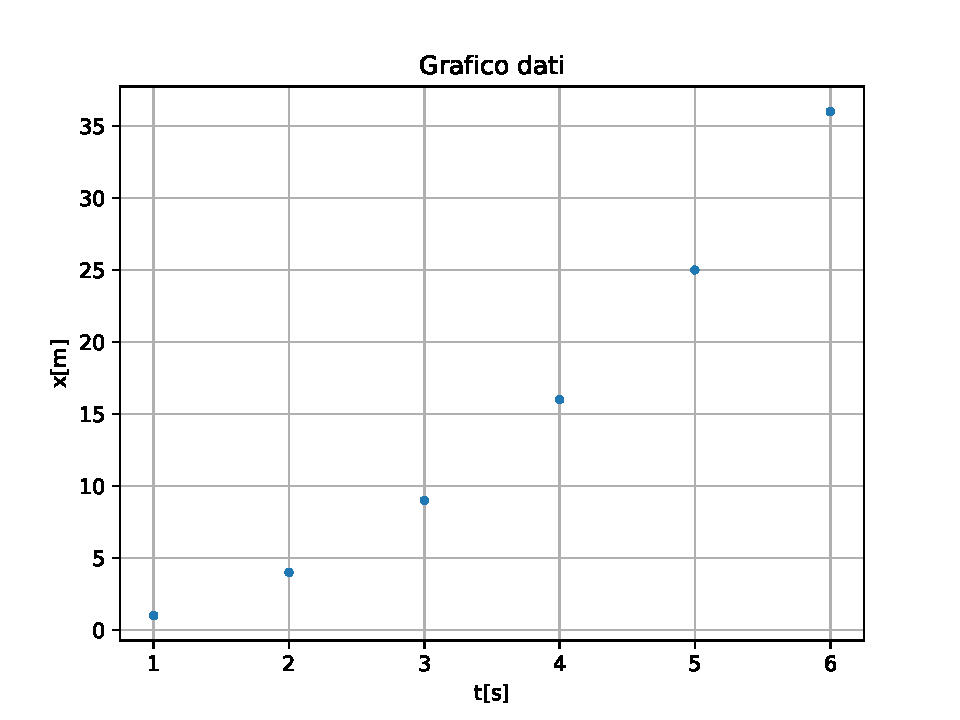
\includegraphics[scale=0.5]{img/grafico1.pdf}

\end{multicols}
Commentiamo un attimo quanto fatto: dopo aver letto i dati abbiamo fatto il grafico mettendo sull'asse delle ascisse la colonna del tempo e su quello delle ordinate la colonna dello spazio; se all'interno del comando "plt.plot(...)" scambiassimo l'ordine di dati1 e dati2 all'ora gli assi si invertirebbero, non avremmo più x(t) ma t(x). Inoltre il comando "marker='.'" sta a significare che il simbolo che rappresenta il dato deve essere un punto; mentre il comando "linestyle=''" significa che non vogliamo che i punti siano uniti da una linea (linestyle='-' dà una linea, linestyle='- -' dà una linea tratteggiata).\\
Se invece volessimo graficare una funzione o più definite da codice? Anche qui i comandi sono analoghi:

\begin{lstlisting}[language=Python]
import numpy as np
import matplotlib.pyplot as plt

def f(x):
    """
    restituisce il cubo di un numero
    """
    return x**3
    
def g(x):
    """
    restituisce il quadrato di un numero
    """
    return x**2

#array di numeri equispaziati nel range [-1,1] usiamo:
x = np.linspace(-1, 1, 40)

plt.figure(1) #creiamo la figura

#titolo
plt.title('Grafico funzioni')
#nomi degli assi
plt.xlabel('x')
plt.ylabel('f(x), g(x)')
#plot dei dati
plt.plot(x, f(x), marker='.', linestyle='--', color='blue', label='parabola')
plt.plot(x, g(x), marker='^', linestyle='-', color='red', label='cubica')
#aggiungiamo una leggenda
plt.legend(loc='best')
#aggiungiamo una griglia
plt.grid()
#comando per mostrare a schermo il grafico
plt.show()
\end{lstlisting}
\begin{multicols}{2}

Notare che per distinguere le due funzioni oltre al "marker" e al "linestyle" abbiamo aggiunto il comando "color" per dare un colore e il comando "label" che assegna un'etichetta poi visibile nella legenda (loc='best' indica che Python la mette dove ritiene più consono, in modo che non rischi magari di coprire porzioni di grafico). Ovviamente è consigliata una lettura della documentazione per conosce tutti gli altri comandi possibili per migliorare/abbellire il grafico da adre alle funzioni già presenti. Altre funzioni utili possono essere: "plt.axis(...)" che imposta il range da visualizzare su entrambi gli assi; il comando "plt.xscale(...)" che permette di fare i grafici con una scala, magari logaritmica o altro sull'asse x (analogo sarà sulle y mutatis mutandis). 


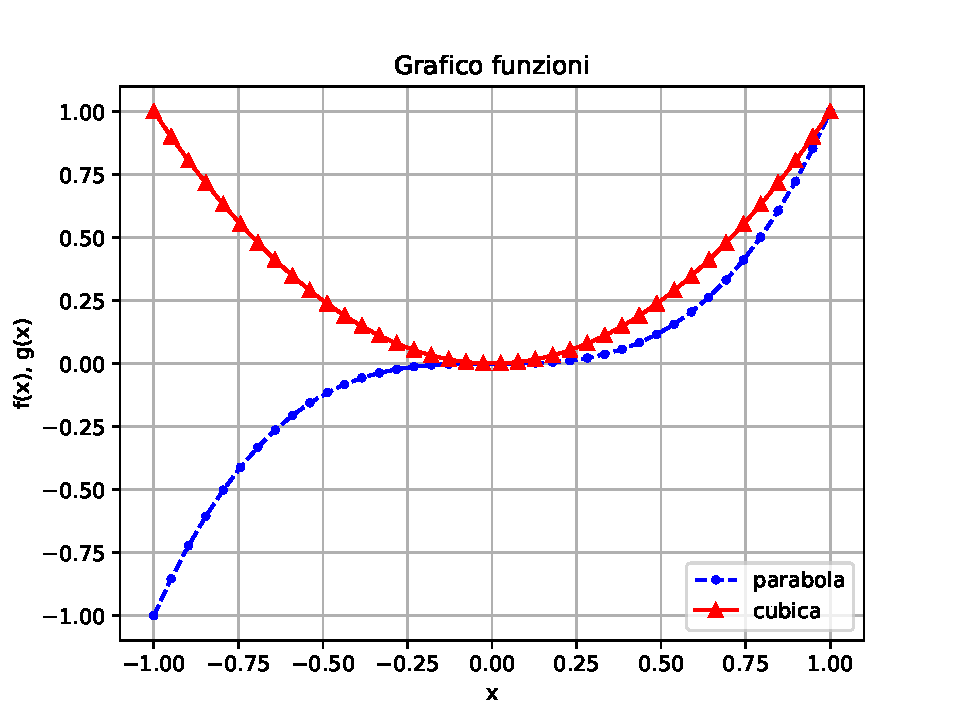
\includegraphics[scale=0.5]{img/grafico2.pdf}

\end{multicols}
Ultima menzione da fare sono gli istogrammi:

\begin{lstlisting}[language=Python]
import numpy as np
import matplotlib.pyplot as plt

plt.figure(1)
plt.title('grafico a barre')
plt.xlabel('valore')
plt.ylabel('conteggi')
# Sull'asse x utilizziamo un array di 10 punti equispaziati.
x = np.linspace(1,10,10)
# Sull'asse y abbiamo, ad esempio, il seguente set di dati:
y = np.array([2.54, 4.78, 1.13, 3.68, 5.79, 7.80, 5.4, 3.7, 9.0, 6.6])

# Il comando per la creazione dell'istogramma corrispondente e':
plt.bar(x, y, align='center')

plt.figure(2)
plt.title('istogramma di una distribuzione gaussiana')
plt.xlabel('x')
plt.ylabel('p(x)')

"""
lista di numeri distribuiti gaussianamente con media 0 e varianza 1
si usa l'underscore nel for poiche' non serve usare
un'altra variabile. Avremmo potuto scrivere for i ...
ma la i non sarebbe comparsa da nessun' altra parte
sarebbe stato uno spreco
"""
z = [np.random.normal(0, 1) for _ in range(int(1e5))]
plt.hist(z, bins=50, density=True, histtype='step')
plt.minorticks_on() # tick piccoli sugli assi

plt.show()
\end{lstlisting}
Piccolo appunto che bisogna fare, nel caso di "plt.hist()" bisogna stare attenti perché il numero di bin va scelto con cura (qui abbiamo scritto 50 sulla fiducia).  

\begin{multicols}{2}


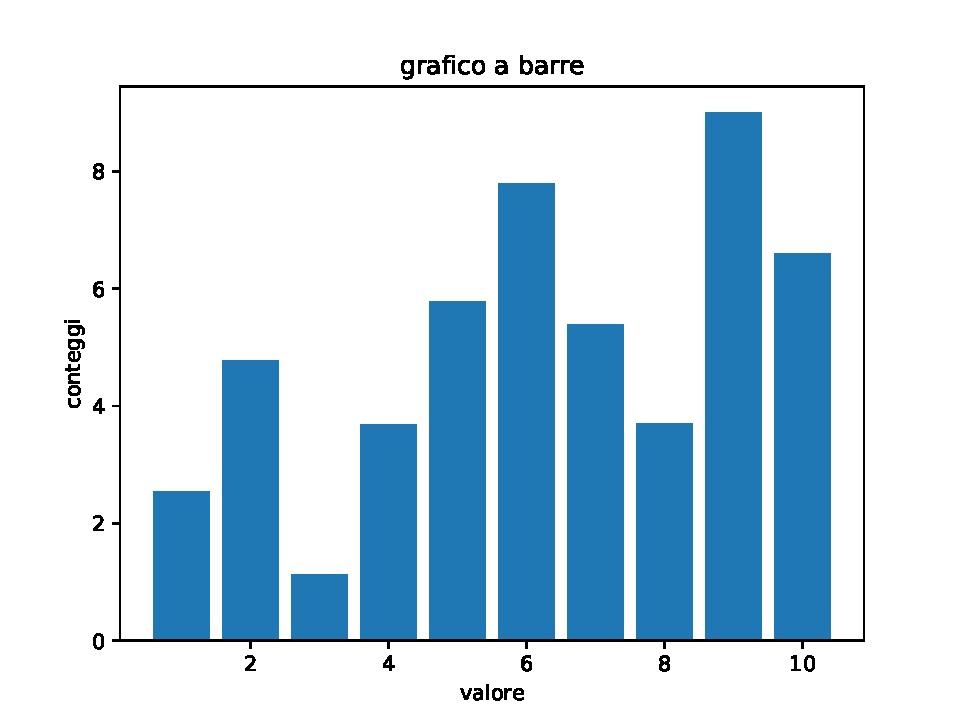
\includegraphics[scale=0.5]{img/isto1.pdf}


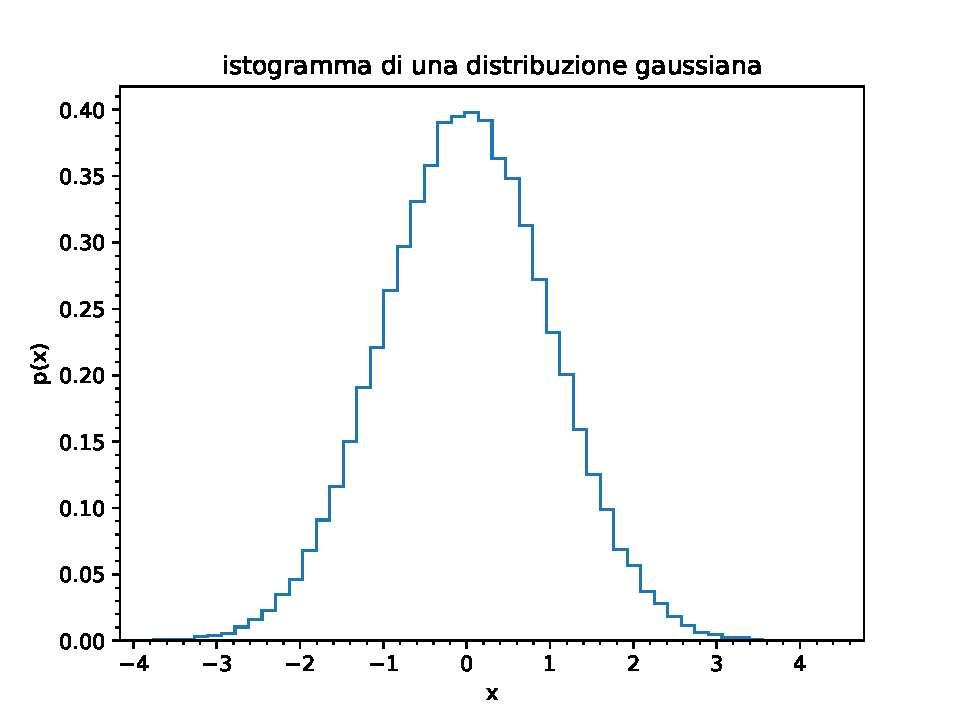
\includegraphics[scale=0.5]{img/isto2.pdf}


\end{multicols}

\subsection{Standard input}
È (a proposito, la È si fa premendo Alt+0200 sul tastierino, quantomeno su windows) inoltre possibile dare la codice che abbiamo scritto degli input da shell. Esistono due modi per farlo: l'uso della funzione "input()", oppure utilizzare "argparse" per dare al codice ciò che serve direttamente da linea di comando su shell, ad esempio se fossimo su una partizione linux senza un editor stile pyzo. Cominciamo con la prima possibilità:
\begin{lstlisting}[language=Python]
"""
Programma per calcolare il trinagolo di tartaglia
"""
import numpy as np

# leggo da input un valore e lo rendo intero
# la stringa verra stampata su shell
n = int(input("Ordine del triangolo: "))
a = np.zeros((n, n), dtype=int) # matrice per i coefficienti

# calocolo i coefficienti del trinagolo
a[0,0] = 1
for i in range(1, n):
    a[i, 0] = 1
    for j in range(1, i):
        a[i, j] = a[i-1, j-1] + a[i-1, j]
    a[i,i] = 1

# stampo a schermo
for i in range(n):
    for j in range(i+1):
    		# solo per fare la forma a piramide
        if j == 0 : # non funziona con numeri a due cifre
            print(*[""]*(n-i),a[i, j], end='')
        else:
            print("",a[i, j], end='')
     print()

[Output]
Ordine del triangolo: 5
     1
    1 1
   1 2 1
  1 3 3 1
 1 4 6 4 1
\end{lstlisting}
Vediamo ora come usare argparse. Ora però il codice è più comodo eseguirlo su una shell, che sia quella di anaconda o quella della vostra distro linux è uguale. Le modifiche al codice sono veramente poche:
\begin{lstlisting}[language=Python]
"""
Programma per calcolare il trinagolo di tartaglia
"""
import argparse
import numpy as np

description='Programma per calcolare il trinagolo di tartaglia leggendo le informazioni da linea di comando'
# descrizione accessibile con -h su shell
parser = argparse.ArgumentParser(description=description)
parser.add_argument('dim',  help='Dimensione della matrice, ovvero potenza del binomio')
args = parser.parse_args()
n = int(args.dim) # accedo alla variabile tramite il nome messo a linea 10

a = np.zeros((n, n), dtype=int) # matrice per i coefficienti

# calocolo i coefficienti del trinagolo
a[0,0] = 1
for i in range(1, n):
    a[i, 0] = 1
    for j in range(1, i):
        a[i, j] = a[i-1, j-1] + a[i-1, j]
    a[i,i] = 1

# stampo a schermo
for i in range(n):
    for j in range(i+1):
        # solo per fare la forma a piramide
        if j == 0 : # non funziona con numeri a due cifre
            print(*[""]*(n-i),a[i, j], end='')
        else:
            print("",a[i, j], end='')
    print()
\end{lstlisting}
Vi metto uno screen della shell per capire cosa è successo (un po' sgranata ma pazienza):

\begin{center}
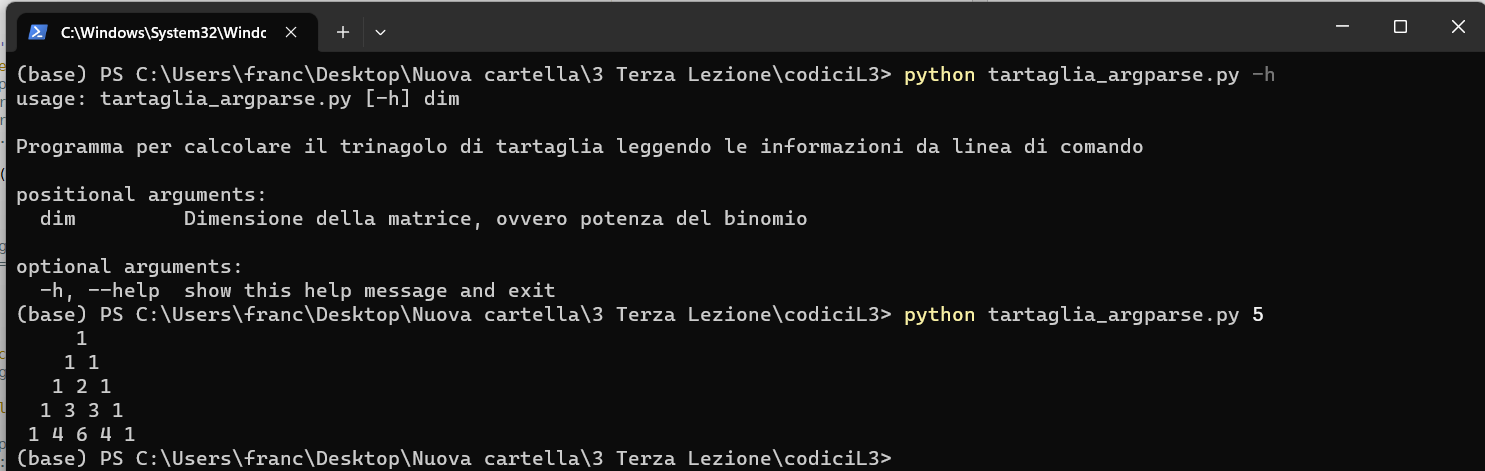
\includegraphics[scale=0.4]{img/shell_argparse.png}
\end{center}

\subsection{Prestazioni: \textit{pure} Python vs librerie}
Avevamo accennato al fatto che Python fosse lento ma che utilizzando le librerie si potesse un po' migliorare le prestazioni, vediamo un esempio:

\begin{lstlisting}[language=Python]
import time
import numpy as np

#inizio a misurare il tempo
start = time.time()


a1 = 0       #variabile che conterra' il risultato
N = int(5e6) # numero di iterazioni da fare = 5 x 10**6

#faccio il conto a 'mano'
for i in range(N):
    a1 += np.sqrt(i)

#finisco di misurare il tempo
end = time.time()-start

print(end)

#inizio a misurare il tempo
start = time.time()

#stesso conto ma fatto tramite le librerie di python
a2 = sum(np.sqrt(np.arange(N)))

#finisco di misurare il tempo
end = time.time()-start

#sperabilmente sara' minore del tempo impiegato prima
print(end)

[Output]
11.588378429412842
0.8475463390350342
\end{lstlisting}
Vediamo che quindi usando le funzioni di numpy, (np.arange) e le funzioni della libreria standard di Python (sum), è possibile fare lo steso conto in un tempo molto minore che tramite un ciclo for. Questo perché le librerie non sono totalmente in Python ma in molta parte in C e/o fortran.

\subsection{Prestazioni: globale vs locale}
Dedicato a Mattia che non vuole usare le funzioni. Rimanendo però nell'ambito di \textit{pure} Python, si può comunque migliorare le prestazioni del codice. Infatti un codice scritto all'interno di una funzione esegue più velocemente rispetto alle stesse righe scritte in globale.
\begin{lstlisting}[language=Python]
import timeit

start = timeit.default_timer()

for i in range(int(1e8)):
    pass

end = timeit.default_timer() - start

print(f"Tempo in gloable = {end}")

def f():
    for i in range(int(1e8)):
        pass

start = timeit.default_timer()
f()
end = timeit.default_timer() - start

print(f"Tempo in locale  = {end}")

[Output]
Tempo in gloable = 2.915754556655884
Tempo in locale  = 1.5078275203704834
\end{lstlisting}
Se prima la scusa era l'utilizzo delle librerie scritte in C ora dov'è la magagna? Adiamo a fare una cosa molto poco capibile, disassembliamo il codice. Ovvero vediamo il bytecode corrispondente al nostro codice. Infatti l'interprete di Python è una macchina virtuale che esegue il bytecode. Per farlo usiamo la libreria "dis".

\begin{lstlisting}
  5           0 LOAD_NAME                0 (range)
              2 LOAD_NAME                1 (int)
              4 LOAD_CONST               0 (100000000.0)
              6 CALL_FUNCTION            1
              8 CALL_FUNCTION            1
             10 GET_ITER
        >>   12 FOR_ITER                 2 (to 18)
             14 STORE_NAME               2 (i)

  6          16 JUMP_ABSOLUTE            6 (to 12)

  5     >>   18 LOAD_CONST               1 (None)
             20 RETURN_VALUE
\end{lstlisting}
\begin{lstlisting}
 14           0 LOAD_GLOBAL              0 (range)
              2 LOAD_GLOBAL              1 (int)
              4 LOAD_CONST               1 (100000000.0)
              6 CALL_FUNCTION            1
              8 CALL_FUNCTION            1
             10 GET_ITER
        >>   12 FOR_ITER                 2 (to 18)
             14 STORE_FAST               0 (i)

 15          16 JUMP_ABSOLUTE            6 (to 12)

 14     >>   18 LOAD_CONST               0 (None)
             20 RETURN_VALUE
None
\end{lstlisting}
Le righe sopra riportate sono rispettivamente il bytecode delle righe 5 e 6 del codice soprastante prima e della funzione f poi. Vedete che salta subito all'occhio una differenza: per il codice globale alla riga 8 del bytecode c'è scritto STORE\_NAME, mentre per la funzione abbiamo STORE\_FAST. Cosa vuol dire quindi questa differenza? Al di là del fast del nome il punto è che in una funzione le variabili locali vengono salvate in un array di dimensione fissa, non in un dizionario (come avviene con quelle globali). Per cui ci si accede direttamente tramite un indice, rendendo l'operazione molto rapida. Ricordando la scrittura in C a livello base di Python, si tratta semplicemente di una ricerca del puntatore nell'elenco e di un aumento del conteggio dei riferimenti di quello che è la lista, ovvero un PyObject al livello di C, entrambe operazioni altamente efficienti.
Le variabili globali, invece vengono memorizzate in un dizionario. Per cui quando si accede a una variabile globale, Python deve eseguire una ricerca nella tabella hash, che implica il calcolo di un hash e quindi il recupero del valore ad esso associato (non sto adesso a spiegarvi cos'è una tabella hash ma come penso possiate intuire non è altro che una struttura dati a livello di C che permette di utilizzare una corrispondenza chiave-valore). E tutto ciò è più lento.

\subsection{Gestione errori}
È molto facile scrivere codice che produca errore, magari perché distrattamente ci siamo dimenticati qualcosa o magri qualcosa è stato implementato male. Esiste un costrutto che ci permette di gestire gli errori in maniera tranquilla diciamo. Facciamo un semplice esempio:

\begin{lstlisting}[language=Python]
a = 0
b = 1/a
print(b)

[Output]
Traceback (most recent call last):
  File "<tmp 1>", line 5, in <module>
    b = 1/a
ZeroDivisionError: division by zero
\end{lstlisting}
Abbiamo fatto una cosa molto brutta, nemmeno Dio può dividere per zero (al più possiamo appellarci alla censura cosmica e mettere un'orizzonte a vestire la divisione per zero) e quindi il computer ci da errore. Possiamo aggirare il problema, evitando così il second impact, in due modi diciamo:
\subsubsection{Try e except}
Possiamo utilizzare il costrutto try except dicendo al computer: prova a fare la divisione e, sia mai funziona, se questa però da errore, e l'errore è "ZeroDivisionError" allora assegna a b un altro valore. In questo modo eventuali istruzioni presenti dopo vengono eseguite e il codice non si arresta.
\begin{lstlisting}[language=Python]
a = 0
try :
    b = 1/a
except ZeroDivisionError:
    b = 1
    
print(b)

[Output]
1
\end{lstlisting}
Anche qui è fondamentale indentare il blocco delle istruzioni.

\subsubsection{Raise Exception}
Mettiamo il caso in cui ci siano operazioni da fare in cui il valore della variabile "b" è importante, quindi sarebbe meglio interrompere il flusso del codice perché con un dato valore il risultato finale sarebbe poco sensato. Si può fare il controllo del valore e sollevare un'eccezione per fermare il codice.
\begin{lstlisting}[language=Python]
"""
leggo un valore da shell
uso del comando try per evitare che venga letto
qualcosa che non sia un numero: e.g. una stringa
"""
try:
    b = int(input('scegliere un valore:'))
except ValueError:
    print('hai digitato qualcosa diverso da un numero, per favore ridigitare')
    b = int(input('scegliere un valore:'))
    
#se si sbaglia a digitare di nuovo il codice si arresta per ValueError

#controllo se e' possibile proseguire
if b > 7 :
    #se vero si blocca il codice sollevando l'eccezione
    messaggio_di_errore = 'il valore scelto risulta insensato in quanto nulla supera 7, misura massima di ogni cosa'
    raise Exception(messaggio_di_errore)

[Output]
8
Traceback (most recent call last):
  File "<tmp 1>", line 18, in <module>
    raise Exception(messaggio_di_errore)
Exception: il valore scelto risulta insensato in quanto nulla supera 7, misura massima di ogni cosa
\end{lstlisting}

\subsection{Logging}
Supponiamo voi abbiate un certo codice, che fa delle certe cose. Per verificare che tutto stia andando bene quello che in genere facciamo e mettere dei "print" in giro per il codice facendoci stampare qualche quantità per vedere se il suo valore sia qualcosa dotato di una parvenza di senso. Possiamo però anche fare qualcosa di un pochetto più sofisticato. Avete presente che quando scrivete in latex, dopo aver compilato, vi compaiono diversi file? Avete mai notato che uno di questi ha l'estensione ".log"? Quel file contiene tutte le informazioni di ciò che è successo durante la compilazione, che siano errori, warning o che tutto sia andato liscio. La libreria "logging" ci per mette di fare una cosa analoga; e questo ci aiuta nella gestione degli errori, nel debug, nel verificare che tutto funzioni come deve. Iniziamo con il dire che in logging esistono 5 livelli: \\
\begin{itemize}
\item DEBUG: quando servono informazioni dettagliate per fare diagnostica.
\item INFO: quando vogliamo conferma che tutto sta andando come deve.
\item WARNING: quando succede qualcosa di non molto grave, il codice comunque pò continuare ad andare.
\item ERROR: c'è un errore, qualche comando non funziona.
\item CRITICAL: veramente grave il codice non può continuare a runnare.
\end{itemize} 
\begin{lstlisting}[language=Python]
import logging

# configuro il formato del logging; voglio sapere: il tempo, il nome del logger, il livello, e il messaggio
logging.basicConfig(level=logging.INFO, format='%(asctime)s - %(name)s - %(levelname)s - %(message)s')

def divisione(x, y):
    """ Funzione particolarmente complicata
    """
    return x / y

# codice particolarmente complicato
x_1 = 17
x_2 = 4

quoziente = divisione(x_1, x_2)

# controllo che tutto sia andato bene via print
print(f"{x_1} / {x_2} = {quoziente}")

# Controllo che tutto sia andato bene via logging, la stringa sara' il messaggio
logging.info(f"{x_1} / {x_2} = {quoziente}")

[Output]
17 / 4 = 4.25
2024-01-11 14:42:43,998 - root - INFO - 17 / 4 = 4.25
\end{lstlisting}
Vediamo che succede. Cominciamo con il dire che dei 5 livelli elencati prima, quello di default è WARNING. Il che implica che eventuali "logging.debug/logging.info" non verebbero stampati. A linea 4 noi settiamo il livello ad INFO, in modo che "logging.info" funzioni. Specifichiamo poi un formato del messaggio con alcune caratteristiche che possono essere di nostro interesse. Possiamo anche aggiungere altre informazioni che volendo trovate sula documentazione. Se vogliamo rimandare l'output su file basta aggiungere due voci a "basic.Config":  
\begin{lstlisting}[language=Python]
import time
import logging

# configuro il formato del logging; voglio sapere:
#il tempo, il nome del logger, il livello, e il messaggio
# Inoltre piuttosto che su shell deve essere stampato su un file,
#che deve essere sovrascritto ad ogni esecuzione del codice
logging.basicConfig(level=logging.INFO, 
                    format='%(asctime)s - %(name)s - %(levelname)s - %(message)s', 
                    filename="file.log", filemode="w") # filemode di default e' a (append)

def divisione(x, y):
    """ Funzione particolarmente complicata
    """
    return x / y

# codice particolarmente complicato
for i, j in zip(range(15, 30), range(1, 16)):

    quoziente = divisione(i, j)

    # Controllo che tutto sia andato bene via logging, la stringa sara' il messaggio
    logging.info(f"{i} / {j} = {quoziente}")
    time.sleep(1)
\end{lstlisting}
Avrete un file di questo tipo:
\begin{lstlisting}[language=Python]
2024-01-11 15:01:27,827 - root - INFO - 15 / 1 = 15.0
2024-01-11 15:01:28,829 - root - INFO - 16 / 2 = 8.0
2024-01-11 15:01:29,830 - root - INFO - 17 / 3 = 5.666666666666667
2024-01-11 15:01:30,831 - root - INFO - 18 / 4 = 4.5
2024-01-11 15:01:31,833 - root - INFO - 19 / 5 = 3.8
2024-01-11 15:01:32,835 - root - INFO - 20 / 6 = 3.3333333333333335
2024-01-11 15:01:33,837 - root - INFO - 21 / 7 = 3.0
2024-01-11 15:01:34,837 - root - INFO - 22 / 8 = 2.75
2024-01-11 15:01:35,839 - root - INFO - 23 / 9 = 2.5555555555555554
2024-01-11 15:01:36,841 - root - INFO - 24 / 10 = 2.4
2024-01-11 15:01:37,843 - root - INFO - 25 / 11 = 2.272727272727273
2024-01-11 15:01:38,844 - root - INFO - 26 / 12 = 2.1666666666666665
2024-01-11 15:01:39,846 - root - INFO - 27 / 13 = 2.076923076923077
2024-01-11 15:01:40,847 - root - INFO - 28 / 14 = 2.0
2024-01-11 15:01:41,849 - root - INFO - 29 / 15 = 1.9333333333333333
\end{lstlisting}
Quindi capite bene che è un ottimo modo per verificare il funzionamento del codice. Magari se il codice richiede tempo è meglio che l'output sia su shell. Per finire supponiamo che voi abbiate due codici che usate insieme, importando uno nell'altro magari (vedere l'inizio della prossima lezione), e che entrambi usino il logging. Utilizzare semplicemente "logging.basicConfig" potrebbe causare problemi in quanto non si specifica il nome del logger, ed entrambi hanno root di default. Quindi in sostanza potrebbe capitare che su shell, o su file, solo le informazioni di un codice vengano scritte. Vediamo quindi un altro modo di settare il logger.
\begin{lstlisting}[language=Python]
import time
import logging

# Creo il logger, __name__ e' il nome del codice ed e' __main__ se viene eseguito, __module__ se importato
logger = logging.getLogger(__name__)

# Settiamo il livello ad INFO, vogliamo controllare che vada tutto bene
logger.setLevel(logging.INFO)

# Settiamo il formato del messaggio di log
formatter = logging.Formatter('%(asctime)s - %(name)s - %(levelname)s - %(message)s')

# Creiamo il gestore del file
file_handler = logging.FileHandler('error.log', mode="w")
file_handler.setLevel(logging.ERROR) # Settiamo un livello diverso per il file 
file_handler.setFormatter(formatter) # sul file ci saranno solo i messaggi di errore

# Vogliamo vedere tutto anche su shell
stream_handler = logging.StreamHandler()
stream_handler.setFormatter(formatter)

# Aggiungiamo tutto al nostro logger
logger.addHandler(file_handler)
logger.addHandler(stream_handler)

#================= main del codice =================

def divisione(x, y):
    """ Funzione particolarmente complicata
    """
    try :
        q = x / y
    
    except ZeroDivisionError:
        # logger.error restituisce solo il messaggio scritto da noi
        #logger.error('Qualcosa e' andato storto si stava per verificare il second impact')
        
        # logger.exception ci resistuisce anche tutto il traceback
        logger.exception("Qualcosa stava andando storto si stava per verificare il second impact")
    
    else :
        return q

# codice particolarmente complicato
for i, j in zip(range(15, 30), range(0, 15)):

    quoziente = divisione(i, j)

    logger.info(f"{i} / {j} = {quoziente}")
    time.sleep(1)

[Output]
2024-01-11 22:05:25,178 - __main__ - ERROR - Qualcosa stava andando storto si stava per verificare il second impact
Traceback (most recent call last):
  File "/home/francesco/GitHub/4BLP/3 Terza Lezione/logging3.py", line 32, in divisione
    q = x / y
ZeroDivisionError: division by zero
2024-01-11 22:05:25,178 - __main__ - INFO - 15 / 0 = None
2024-01-11 22:05:26,180 - __main__ - INFO - 16 / 1 = 16.0
2024-01-11 22:05:27,181 - __main__ - INFO - 17 / 2 = 8.5
2024-01-11 22:05:28,182 - __main__ - INFO - 18 / 3 = 6.0
2024-01-11 22:05:29,183 - __main__ - INFO - 19 / 4 = 4.75
2024-01-11 22:05:30,184 - __main__ - INFO - 20 / 5 = 4.0
2024-01-11 22:05:31,185 - __main__ - INFO - 21 / 6 = 3.5
2024-01-11 22:05:32,187 - __main__ - INFO - 22 / 7 = 3.142857142857143
2024-01-11 22:05:33,188 - __main__ - INFO - 23 / 8 = 2.875
2024-01-11 22:05:34,190 - __main__ - INFO - 24 / 9 = 2.6666666666666665
2024-01-11 22:05:35,192 - __main__ - INFO - 25 / 10 = 2.5
2024-01-11 22:05:36,194 - __main__ - INFO - 26 / 11 = 2.3636363636363638
2024-01-11 22:05:37,196 - __main__ - INFO - 27 / 12 = 2.25
2024-01-11 22:05:38,197 - __main__ - INFO - 28 / 13 = 2.1538461538461537
2024-01-11 22:05:39,199 - __main__ - INFO - 29 / 14 = 2.0714285714285716
\end{lstlisting}
Vediamo quindi che ora il logger si chiama \_\_main\_\_ e che tutto viene stampato correttamente su shell. Notiamo che c'è un errore ma il codice poi continua ad eseguire, quindi magari il messaggio sparirà poi, però noi lo abbiamo scritto anche sul file. Quindi il file "error.log" contiene le prime righe dell'output, così possiamo andare a vedere ne capire che succede e poi risolvere in caso. Giusto per chiarire: noi abbiamo scritto "logging.getLogger(\_\_name\_\_)" per distinguere tra codice ed eventuale modulo, ma nulla ci vieta di chiamare il logger in modo diverso (magari se abbiamo più codici e vogliamo distinguere la sorgente del messaggio); basta passargli una stringa: "logging.getLogger('Ajeje')".
\subsection{Generatori}
Abbiamo visto che strutture dati quali liste, tuple, array eccetera sono degli iterabili e possiamo quindi usarli per scorrerci sopra. Tutto ciò può, però essere fatto con i generatori. Ovvero delle funzioni che piuttosto avere la keyword "return" hanno "yield". Scrittà così, una funzione dopo aver fatto i suoi conti non temrina ma viene sospesa, finchè non servirà chiamarla nuovamente per ottenere il valore successivo. Queste funzioni si chiamano appunto funzione generatore o generatori iteratori. Per accedere agli elementi che essa restistuisce possiamo ciclarci sopra oppure usare la funzione "next()" che vedremo più avanti. Vediamo un piccolo esempio:
\begin{lstlisting}[language=Python]
"""
Codice esempio di utilizzo yield per un generatore
"""

def generatore():
    ''' funzione generatore
    '''
    yield 1
    yield 2
    yield 3

gen = generatore()

for val in gen:
    print(val)

[Output]
1
2
3
\end{lstlisting}
Vedete che quindi è come fosse uno di quei range che usiamo in genere nei cicli for. Se infatti provate a stampare la variabile "gen" vedrete che essa non stamperà: 1, 2, 3. Vediamo ora appunto il confronto con range:
\begin{lstlisting}[language=Python]
"""
Codice esempio di utilizzo yield e confronto con range
"""

def generatore(N):
    '''
    Funzione generatore

    Parameter
    ---------
    N : int
        limite fino a cui arrviare
    '''
    n = 0
    while n < N:
        yield n
        n += 1

for val_g, val_r in zip(generatore(10), range(10)):
    print(val_g, val_r)

[Output]
0 0
1 1
2 2
3 3
4 4
5 5
6 6
7 7
8 8
9 9
\end{lstlisting}
Vedete che le due funzioni si comportano allo stesso modo. Ma perchè usare le funzioni con "yield"? Il motivo sta in quello che abbiamo detto prima, la funzione non ritorna una lista o altro di simile contennete tutti i valori che ci interessano ma ci da un solo valore alla volta senza terminare l'esecuzione della funzione ma semplicemente mettendola in pausa. Vedete che quindi ciò permette ai nostri codici di allocare molta meno ram. Vediamo un effettivo esempio di quanta ram si utilizzi in questi contesti:
\begin{lstlisting}[language=Python]
"""
Codice per verificare il consumo di ram
"""

import sys

N = int(2e8) # quanti numeri generare 2 x 10**8

def gen(N):
    '''
    Funzione generatore

    Parameter
    ---------
    N : int
        limite fino a cui arrviare
    '''
    for i in range(N):
        yield i

# Conservo una tutto in una lista
n_l = list(gen(N))

# Definisco semplicemente il generatore
n_g = gen(N)

def size(obj):
    '''
    Funzione per calcolare tutta la memoria di un ogetto

    Parameter
    ---------
    obj : list, tuple, set, dict
        python object
    '''
    Size = sys.getsizeof(obj)

    # se e' una lista tupla o set
    if isinstance(obj, (list,tuple,set)):
        for el in obj:
            Size += size(el)

    # se e' un dizionario devo considerare sia chiave che valore
    if isinstance(obj, dict):
        for k, v in obj.items():
            Size += size(k)
            Size += size(v)

    return Size

print(f"Dimensione della lista:    {size(n_l)} byte")

del n_l # elimino la variabile dalla memoria in quanto incredibilmente pesante

print(f"Dimensione del generatore: {size(n_g)} byte")

[Output]
Dimensione della lista:    7293045240 byte
Dimensione del generatore: 208 byte
\end{lstlisting}
Analizziamo il codice che abbiamo appena mostrato: abbiamo definito la nostra funzione generatore come nel programma precedente e gli passiamo un valore fino a cui iterare molto grande: $2 \times 10^8$.
La variabile n\_g è semplicemente il generatore che possiamo usare come sopra, mentre in n\_l, grazie all'utilizzo della funzione list, stiamo conservando una lista contenete tutti i numeri su cui potremmo voler iterare (da 0 a $2 \times 10^8$) quindi stiamo allocando dello spazio.
La funzione "size" ci dice quanto pesa un oggetto nella sua totalità. Vediamo quindi che la lista pesa $7.2$ Gigabyte mentre il generatore sono pochi byte, ma entrambe ci permettono di fare le stesse cose. Quindi ecco, vedete che abbiamo un enorme risparmio di ram. Un uso di tali funzioni può essere utile se magari stiamo leggendo riga per riga un file di grosse dimensioni. Impariamo poi una nuova keyword ovvero "del" che ci permette di eliminare una variabile. Qui viene usata per pulire tutta quella ram allocata ed evitare di bloccarmi il pc.
Poi come il mio computer sia riuscito a gestire 7.2 giga in ram con una ram da 6 è dovuto alle magie di Zram, cercate se vi interessa.
\subsubsection{Problema delle 8 regine}
Vediamo un'applicazione carina dell'utilizzo di "yield". Il problema delle otto regine consta nel trovare le disposizioni possibili in cui collocare 8 regine in una scacchiera 8$\times$8 senza che esse si minaccino  vicenda. Vediamo come tutto ciò può essere fatto facilmente grazie a "yield":
\begin{lstlisting}[language=Python]
"""
Codice per risolvere il problema delle N regine in una scacchiera N x N
"""
import matplotlib.pyplot as plt


def queens(n, i=0, col=[], diag_sup=[], diag_inf=[]):
    '''
    Codice che genera le configurazioni delle N regine,
    la funzione e' un generatore quindi non restituisce
    tuttle le configurazioni ma le calcola man mano

    Parameters
    ----------
    n : int
        quante regine vanno piazzate
    i : int
        numero di regine piazzate
    col : list
        lista che contiene la posizione della regina
        nelle varie colonne.
    diag_sup : list
        lista per controllare le diagonali in salita
    diag_inf : list
        lista per controllare le diagonali in discesa
    '''

    # Finche' non sono piazzate N regine
    if i < n:
        # Ciclo sulle posizioni
        for j in range(n):
            # se la regina non e' nella colnna e non ci stanno delle regine
            # a minacciare la casella lungo le diagonali, chiamo ricorsivamente
            if j not in col and i + j not in diag_sup and i - j not in diag_inf:
                # richiamo avendo fissato una regina nella posizione j
                yield from queens(n, i + 1, col + [j], diag_sup + [i + j], diag_inf + [i - j])
    else:
        yield col


def plot_queens(board):
    '''
    Funzione per plottare la scacchiera

    Parameter
    ---------
    board : list
        lista delle posizioni, ouput della funzione queens
    '''
    n = len(board)

    # Creo la scacchiera
    chessboard = [[(i + j) % 2 for i in range(n)] for j in range(n)]
    plt.imshow(chessboard, cmap='binary')

    # Metto le regine
    for i in range(n):
        plt.text(i, board[i], 'Q', color='red', ha='center', va='center', fontsize=20)

    plt.yticks(range(n), [i for i in range(n, 0, -1)])
    plt.xticks(range(n), [chr(i) for i in range(97, 97+n)])
    plt.show()


def select(N):
    '''
    funzione per selezionare l'N-esima configurazione
    '''
    Q = queens(8)
    for i in range(N-1):
        next(Q)

    return next(Q)

B = select(11)
plot_queens(B)
\end{lstlisting}
Vediamo qui inoltre l'utilizzo della funzione "next" a cui accennavamo prima. Per selezionare la configurazione di nostro interesse mandiamo avanti con "next" lo stato del generatore per quanto ci interessa. Vediamo anche il plot che è carino.

\begin{center}
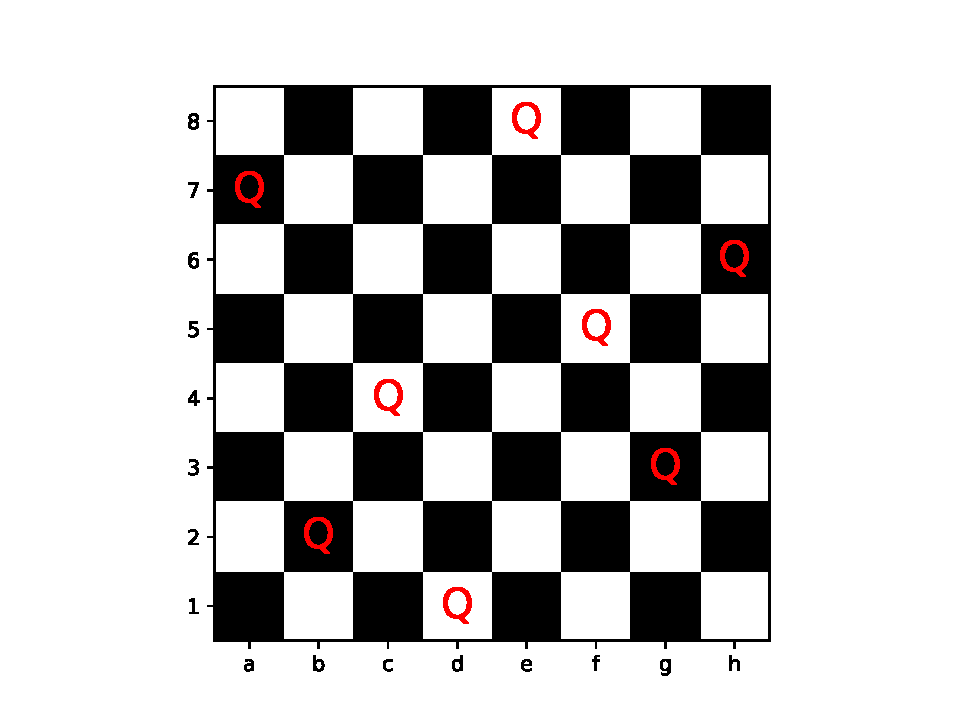
\includegraphics[scale=0.7]{img/8Q.pdf}
\end{center}

\subsection{Esercizi}
Anche qui voglio lasciarvi qualche esercizio per farvi prendere confidenza con quanto imparato finora. Ci saranno però delle modifiche. Infatti di alcuni esercizi non vi darò la soluzione ma solo un file che testa la vostra proposta di soluzione. Tale test vi darà un paio di info sul vostro codice, ad esempio la memoria che esso utilizza, il tempo che impiega, ed anche implementato il test tramite pylint. Si tratta di un pacchetto molto interressante che analizza la sintassi del vostro codice secondo quelle che sono le regole canoniche di scrittura, vi evidenzia gli errori e vi da una valutazione. Mi raccomando se nel testo dell'esercizio vi dico di chiamare una funzione in un certo modo, fatelo, così il codice test può fare i confronti del caso. Tale file di test sarà un codice python chiamato "test.py" che potete eseguire normalmente evi si aprirà la finestra. I più corraggiosi posso cimentarsi nel leggere e capire tale codice volendo "\textit{audentes fortuna iuvat}". Vi faccio vedere sotto, alla soluzione del primo esercizio, come appare la finestra del test.\\
\begin{enumerate}
\item Scrivere una funzione "area(l, n)" che calcoli l'area di un poligono regolare di lato 
"l" e numero di lati "n". Scrivere poi una funzione "pitagora(lista\_lati, n)" che prenda in 
input una lista di tre elementi (una terna pitagorica) e un numero di lati "n" e che 
restituisca la somma delle aree delle figure sui cateti a cui sottraete l'area della 
figura sull'ipotenusa. Fatelo magari per vari valori. Di seguito una formula che potrebbe tornarvi utile:
\[
A = \frac{1}{2}(nl)\frac{l \cot(\pi/n)}{2}
\]
\item Fare con un ciclo più plot su uno stesso grafico, dove la funzione deve dipendere dalla variabile su cui si cicla (e.g. $x^i$ con x un array di un certo range e i la variabile del cilo).
\item Stessa cosa di sopra ma ora ogni curva deve avere un colore e uno linstyle diverso e una legenda.
\item Creare una funzione che legga da input un numero intero con la condizione che esso sia maggiore di zero e che dia la possibilità di inserirlo nuovamente finché la condizione non è verificata.
\item Sovrapporre i plot di un istogramma e della funzione di distribuzione associata, a vostra scelta, e aggiungere al grafico tutte le bellurie del caso.
\item Scrivere una funzione "osservabile(data)" che dato un array "data" ne restituisca la media e la deviazione standard in un array.
\[ 
\mu = \sum_i^{n} x_i \quad \sigma =  \sqrt{ \frac{1}{n(n-1)} \sum_i^n (x_i - \mu)^2 } 
\]
\item Scrivere una funzione "pi\_greco\_for(N)" che usi il problmea di basilea per stimare il valore di $\pi$, che deve essere il return della funzione, e deve utilizzare un ciclo for. Scrivere poi la funzione "pi\_greco\_vec(N)" che faccia la stessa cosa ma vettorialmente, quindi senza cicli. (Come N prendete qualcosa del tipo $10^6$).
\[
\frac{\pi}{6} \simeq \sum_{n=1}^N \frac{1}{n^2}
\]
\item Scrivere una funzione "decimal\_to\_binary(n)" che converta un numero intero "n" in base 10 in un numero in base 2; il numero in base due deve esse una stringa (i.e. 10 $\rightarrow$'1010').
\item Scrivere una funzione "binary\_to\_decimal(nb)" che prenda una stringa "nb" rappresentante un numero in base due e lo converta in base 10 (l'inverso del precedente esercizio).
\item Scrivere una funzione "trova\_primi(n)" che dato un numero intero "n" trovi tutti i numeri primi minori di n e li restituisca in un array.
\item Scrivere una funzione "palindromo(n)" che controlli se un numero intero "n" sia palindormo restituendo True se lo è False altrimenti.
\item Scrivere una funzione "cesare(msg, key, enc)" che prenda in input: una stringa "msg" che è il testo da cifrare o da decifrare (con il cifrario di cesare appunto), un intero "key" che è la chiave con cui criptare il messaggio, e una variabile booleana "enc" per stabilire se la funzione debba cifrare o decifrare il messaggio in input, deve restituire in output una stringa che sia il messaggio cifrato o decifrato a seconda. Il perchè della variabile booleana è data dal fatto che se un testo è stato cifrato con la chiave 13 ad esempio, storico valore usato, esso può venir decifrato usando come chiave -13. Come hint sappiate che esistono delle funzioni di python che possono tornarvi utili "ord()", "char()".
\item Scrivere una funzione "dec\_to\_esa(n)" che converta un numero intero "n" in base 10 in un numero in base 16; il numero in base 16 deve esse una stringa (i.e. 158 $\rightarrow$'9E').
\item Scrivere una funzione "esa\_to\_dec(ne)" che prenda una stringa "ne" rappresentante un numero in base 16 e lo converta in base 10 (l'inverso del precedente esercizio).
\item Scrivere una funzione "clean\_data(x)" che prenda in input un array "x" contenente dei nan (potete scriverlo come x=np.array([3, np.nan, 8])) e che restituisca l'array pulito con degli zeri al posto dei nan (nell'esempio precendente [3, 0, 8]).
\item Scrivere una funzione "eq(a, b, c)" che prenda in input tre numeri reali "a", "b", "c" corrispondeti ai coefficienti di un polinomio p(x) di secondo grado e che restituisca gli zeri di tale polinomio in un array. Si consideri $p(x)=ax^2+bx+c$.
\item Scrivere una funzione "fattori(n)" che prenda in input un numero intero "n" e restituisca una lista contenente la sua scomposizione in fattori primi, con la loro molteplicità (i.e. 20 $\rightarrow$ [2, 2, 5]). 
\item Scrivere una funzione "goldbach(n)" che prenda in input un numero intero "n" e restituisca una lista di tuple, ciascuna delle quali contenente due numeri primi che sommati danno "n" (i.e. 10 $\rightarrow$ [(3, 7), (5, 5)]).
\item Esiste un semplice algoritmo per il calcolo della radice di un numero. Si chiama algoritmo di Newton e fornisce un regola iterativa per approssimare la radice data una certa tolleranza. Vediamo tale regola:
\[
\begin{split}
1)& \, \text{ prendo } n = \text{ un certo numero di cui voglio calcolare la radice} \\
2)& \, \text{ pongo } x = n \\
3)& \, \text{ calcolo } x_n = 0.5 (x - n/x) \\
4)& \, \text{ se } | x - x_n | < \text{ una certa tolleranza } \\
5)& \, \text{ altrimenti pongo } x = x_n \text{ e riparto dal punto 3)}
\end{split}
\]
Scrivere quindi una funzione "newton\_sqrt(n, tol)" che prenda un numero reale "n", numero di cui calcolare la radice, e un numero reale "tol" che rappresenta la tolleranza dell'algoritmo (e.g. $10^{-5}$). La funzione deve restituire la radice calcolata.
\item Scrivere una funzione "EMCD(a, b)" che dati due numeri interi "a" e "b" restituisca in un array: il massimo comun divisore di "a" e "b", l'inverso moltiplicativo di "a" modulo b (che chiamiamo X) e l'inverso moltiplicativo di "b" modulo a (che chiamiamo Y). Ovvero vale la seguente identità (di Bézout):
\[
a X + b Y = \text{MCD}(a, b) 
\]
Per farlo utilizzate l'algoritmo esteso di euclide. Questa volta l'algoritmo non ve lo spiego io ma vi lascio ad una facile ricerca su internet.
\end{enumerate}



\FloatBarrier
\begin{figure}
\centering
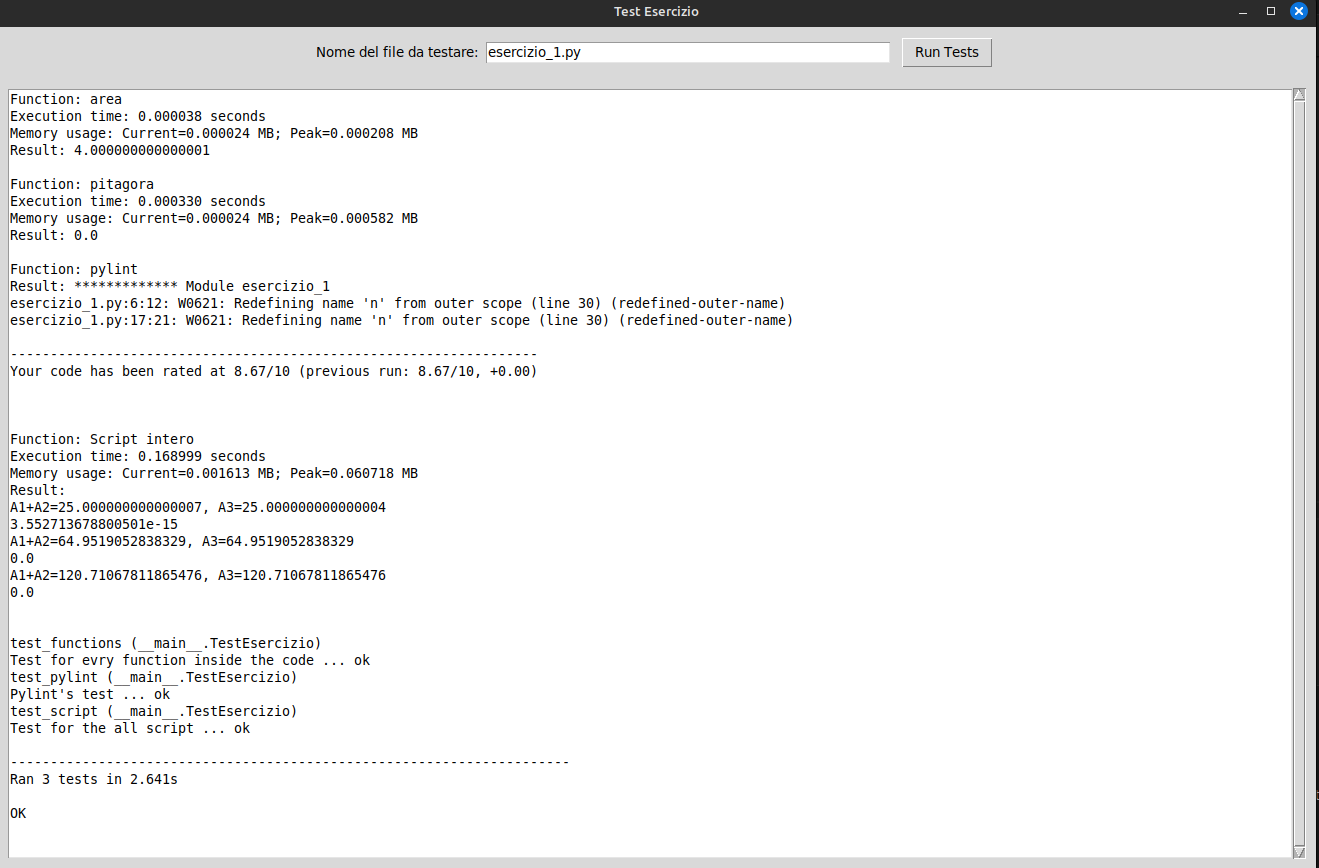
\includegraphics[scale=0.25]{img/ese_test.png}
\caption{Quando eseguirete il test vi si aprirà questra finestra. Voi dovete inserire in nome del file su cui avete svolto l'esercizio e poi premere il tasto sulla finestra dove c'è scritto "Run Tests". Analiziamo ora l'output che ho ottenuto con la mia soluzione: I test delle due funzioni separatamente sono andati a buon fine; Il test di pylint ha riportato dei warning per quanto riguarda la variabile n alla linea 30, ho comunque preso un onesto punteggio 8.67 su 10. Più in basso il test esgue lo script per intero e stampa il risultato che, se eseguissi lo script, verrebbe stampato su shell. Dopodichè la finestra ci dice che il teste delle funzioni e il test dello script è andato bene; quello di pylint sarà sempre ok perchè tanto la cosa importante sono i warning che ha dato sopra e il punteggio.}
\end{figure}
\FloatBarrier
\FloatBarrier
\begin{figure}
\centering
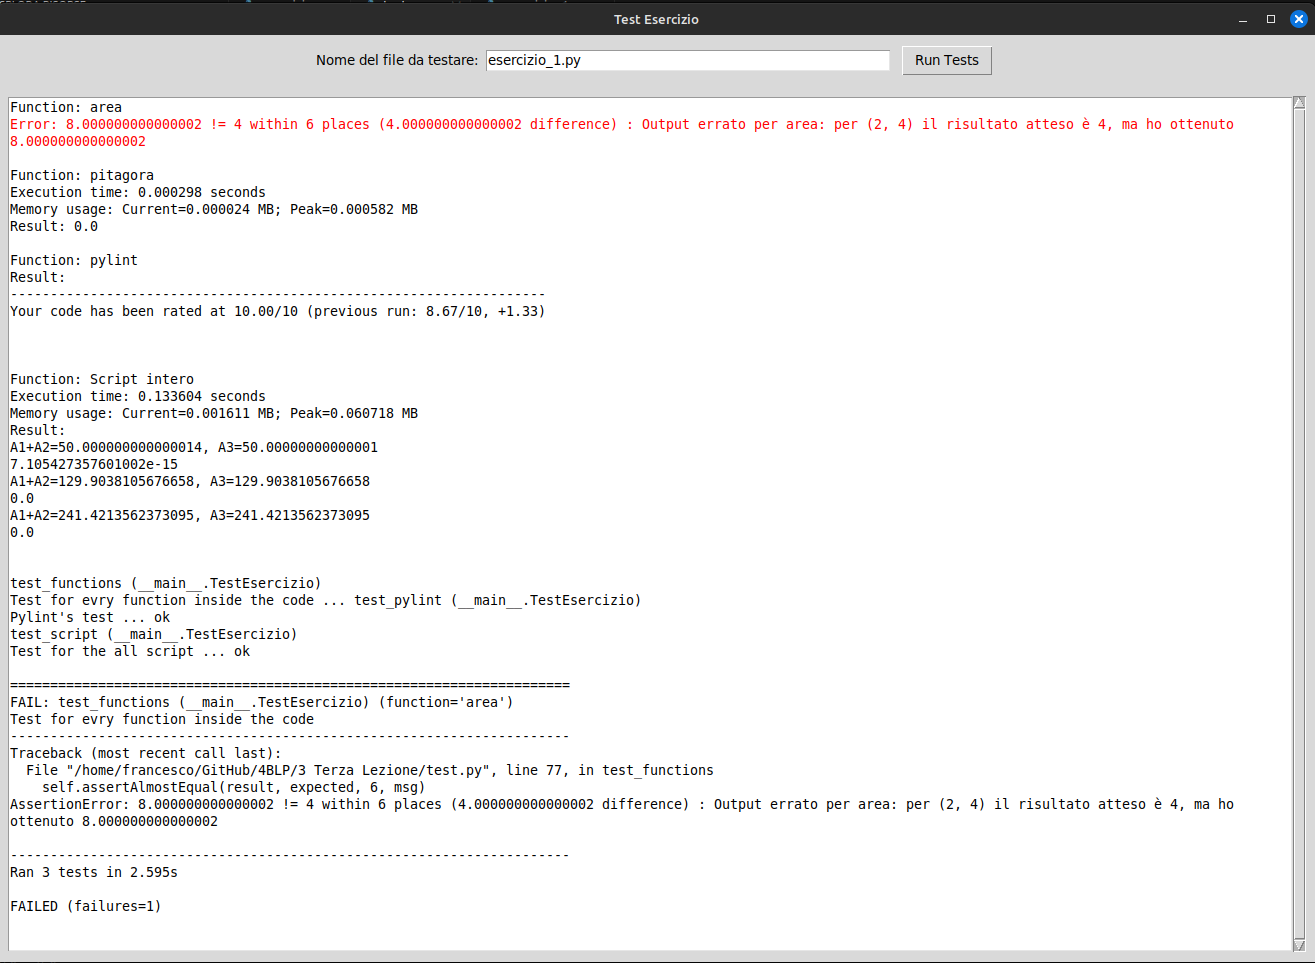
\includegraphics[scale=0.25]{img/ese_test_2.png}
\caption{Qui invece veete come appare il caso di errore. Ho corretto le lagne di pylint ma per sbaglio ho dimenticato un due nella formula dell'area per cui ottengo un errore.}
\end{figure}
\FloatBarrier
\noindent Secondo:
\begin{lstlisting}[language=Python]
power = [0.5, 1, 2]         # potenze
x = np.linspace(0, 1, 1000) # range sulle x

plt.figure(1)
for p in power:
    plt.plot(x, x**p) # un plot alla volta sulla stessa figura

# bellurie
plt.grid()
plt.title("Esercizio 2")
plt.xlabel("x")
plt.ylabel("f(x)")
plt.show()
\end{lstlisting}
Terzo:
\begin{lstlisting}[language=Python]
power = [0.5, 1, 2]                        # potenze
color = ['k', 'r', 'b']                    # colore di ogni curva
lnsty = ['-', '--', '-.']                  # stile di ogni curva
label = [r'$\sqrt{x}$', r'$x$', r'$x^2$']  # nome della curva
x = np.linspace(0, 1, 1000)

plt.figure(1)
for p, c, ls, lb in zip(power, color, lnsty, label):
    # un plot alla volta sulla stessa figura
    plt.plot(x, x**p, c=c, linestyle=ls, label=lb)

#bellurie
plt.grid()
plt.title("Esercizio 3")
plt.xlabel("x")
plt.ylabel("f(x)")
plt.legend(loc='best')
plt.show()
\end{lstlisting}
Quarto:
\begin{lstlisting}[language=Python]
def read():
    '''
    funzione che legge da input un numero con la condizione che esso
    sia maggiore di zero e che dia la possibilita' di inserirlo
    nuovamente finche' la condizione non e' verificata.
    Volendo si puo' generalizzare il codice passando la condizione come input
    '''
    
    while True:  # Il codice deve runnare finche' non inserisco un numero buono
        
        try: # provo a leggere il numero e a renderlo intero
            x = int(input("Iserisci un numero: "))
            
        except ValueError: # se non riesco sollevo l'eccezione
            print(f"Fra ti ho chiesto di mettere un numero") # messaggio di errore
            continue # questo comando fa ripartire il ciclo da capo
        
        if x > 0: # se la lettura e' andata a buon fine verifico la condizione
            return x # se e' verificata ritorno il numero
        else :
            # alrimenti stampo un messaggio di errore
            print("In numero inserito e' minore di zero, sceglierne un altro.")
            continue # e faccio ripartire il ciclo da capo


x = read()
print(f"Il numero letto e': {x}")
\end{lstlisting}
Quinto:
\begin{lstlisting}[language=Python]
# Gaussiana
m = 0
s = 1
z = [np.random.normal(m, s) for _ in range(int(1e5))]

# Plot dati
plt.figure(1)
plt.hist(z, bins=50, density=True, histtype='step', label='dati')
plt.grid()
plt.xlabel("x")
plt.ylabel("P(x)")
plt.title("Distribuzione gaussiana")

# Plot curva
x = np.linspace(-5*s + m, 5*s + m, 1000)
plt.plot(x, np.exp(-(x-m)**2 / (2*s**2))/np.sqrt(2*np.pi*s**2), 'b', label=f"N({m}, {s})")
plt.legend(loc='best')
plt.show()
\end{lstlisting}


\newpage
\section{Quarta lezione}

\subsection{Importare file Python}
Abbiamo visto come utilizzare le librerie, tutto a partire dal comando import. Oltre alle librerie possiamo importare anche altri file Python scritti da noi, magari perché in quel file è implementata una funzione che ci serve. Facciamo un esempio:

\begin{lstlisting}[language=Python]
def f(x, n):
    """
    restituisce la potenza n-esima di un numero x
    Parametri
    ---------
    x, n : float
    
    Return
    ---------
    v : float
        x**n
    """
    
    v = x**n
    
    return v
    
if __name__ == '__main__':
    #test
    print(f(5, 2))
    
[Output]
25
\end{lstlisting}
Abbiamo questo codice che chiamiamo "elevamento.py" che ha implementato la funzione di elevamento a potenza e supponiamo di voler utilizzare questa funzione in un altro codice, possiamo farlo grazie ad import:

\begin{lstlisting}[language=Python]
import elevamento

print(elevamento.f(3, 3))

[Output]
27
\end{lstlisting}
Notiamo nel codice iniziale la presenza dell'if, esso serve per far si che tutto ciò che sia scritto sotto venga eseguito solo se il codice viene lanciato come 'main' appunto e non importato come modulo su un altro codice. In genere l'utilizzo di questa istruzione è buona norma quando si vuol scrivere un codice da importare altrove.

\subsection{Fit}
Nell'ambito della statistica un fit, cioè una regressione lineare o non che sia (dove la linearità è riferita ai parametri della funzione), è un metodo per trovare la funzione che meglio descrive l'andamento di alcuni dati. Nel caso di regressione lineare la procedura da eseguire non è troppo complicata, mentre per la regressione non lineare le cose si fanno parecchio complicate e si utilizzano algoritmi di ottimizzazione.
Se noi abbiamo quindi un modello teorico che ci dice che un corpo cade con una legge oraria della forma $y(t) = h_0 - \frac{1}{2}gt^2$, grazie al fit possiamo trovare i valori dei parametri della leggere oraria, $h_0$ e $g$, che meglio adattano la curva ai dati (nella speranza che escano valori fisicamente sensati, dato che in genere i dati sono di origine sperimentale o simulativa).
In ogni caso comunque l'idea di ciò che va fatto è trovare il minimo della seguente funzione:
\begin{equation}\label{chisq}
S^2(\{ \theta \}_j ) = \sum_i \frac{(y_i - f(x_i; \{ \theta \}_j ))^2}{\sigma_{y_i}^2}
\end{equation}
che nel caso in cui il termine dentro la somma sia distribuito in modo gaussiano allora la quantità $S^2$ è distribuita come un chiquadro, e da qui si potrebbe fare tutta una discussione sulla significatività statistica di quello che andiamo a fare, che ovviamente noi non facciamo.
Analizziamo un attimo questa formula: $S^2$ è in linea di principio una funzione a molte variabili e che restituisce un numero reale. Il termine dentro la somma rappresenta la distanza tra valore del dato e valore della funzione in unità della barra d'errore del dato. Facciamo un esempio visivo per rendere più chiaro il concetto. Consideriamo giusto a titolo di esempio tre punti e due possibili rette che noi possiamo pensare che più o meno approssimino i dati.
\begin{figure}
\centering
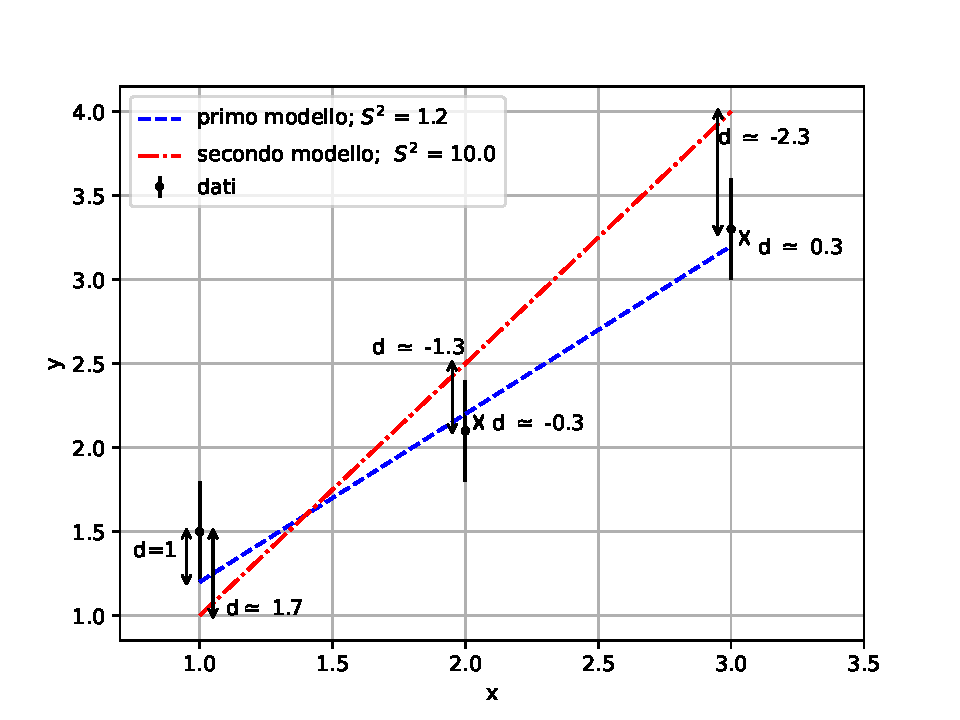
\includegraphics[scale=0.8]{img/chisq_cfr.pdf}
\end{figure}
\FloatBarrier
Nel grafico $d$ è proprio la distanza del modello dal dato in unità di barre di errore, e quindi la somma di tutte queste quantità elevate al quadrato è il valore di $S^2$ che è riportato nella legenda. Notiamo quindi che effettivamente la retta che presenta un valore di $S^2$ minore è quella che ad occhio meglio approssima i dati. Ora uno potrebbe pensare che quindi basta calcolare $S^2$ su una griglia e vedere dove assume il valore più piccolo. Questo è un metodo abbastanza brute force e il linea di principio funziona, ma quello che in genere si fa è un po' diverso. In linea di principio per capire come funziona un algoritmo di minimo basta pensare ad una palline che cade in una ciotola. Precisiamo che si vuole fare tutta questa trattazione per far capire che la parte più delicata di questa procedura è scegliere quello che noi chiameremo nel codice "init" e che esso violentemente aggiusta o complica la nostra situazione. Consideriamo per semplicità, didattica e grafica, una funzione di una singola variabile.
\begin{center}
\begin{tikzpicture}[>=latex]
%\draw[help lines] (0, 0) grid (7, 7);
\begin{axis}
[enlargelimits, xmin=-1,xmax=1,ymin=0,ymax=1,
axis x line=middle,
axis y line=middle]
\addplot [smooth, samples=50, blue] {x^2};
\end{axis}
\fill (6.6, 5.5) circle (0.15);
\node at (4.0, 5.5) {$S^2(x)$};
\draw [dashed, line width=1pt, blue] (6.6, 5.5) -- (6.6, 0);
\draw [->, line width=3pt, blue] (6.6, 5.5) -- (5.8, 3.3);
\node at (5.5, 4.5) {$-\nabla S^2$};
\node at (7, 0.15) {$x_0$};
\fill (5.8, 3.3) circle (0.15);
\draw [dashed, line width=1pt, blue] (5.8, 3.3) -- (5.8, 0);
\draw [->, line width=3pt, blue] (5.8, 3.3) -- (5.2, 2);
\node at (5, 3) {$-\nabla S^2$};
\node at (6, 0.15) {$x_1$};
\fill (5.2, 2) circle (0.15);
\draw [->, line width=3pt, blue] (5.2, 2) -- (4.6, 1);
\end{tikzpicture}
\end{center}
Quel che noi facciamo è scegliere un $x_0$, (il nostro init) ed aggiornare questa posizione considerando la pendenza della funzione, che altro non sarebbe che la derivata della funzione che vogliamo considerare. Concedetemi, per maggiore generalità, si sostituire il termine derivata con il termine gradiente, indicato dal simbolo $\nabla$. Quindi quello che il codice fa è diciamo analogo ad una pallina che si muove sotto l'azione di un potenziale, che sarebbe $S^2$ e la sua derivata, il suo gradiente, non è altro che la forza che la pallina sente. Facendo così troviamo una serie di $x_i$ iterativamente, fino ad arrivare al minimo dove il gradiente, la forza esterna, è zero. Questo metodo è chiamato gradiente discendente. Finché abbiamo un solo minimo quindi va tutto bene. Lo troviamo senza problemi a prescindere da dove partiamo. Supponiamo ora una situazione più brutta:

\begin{center}
\begin{tikzpicture}[>=latex]
%\draw[help lines] (0, 0) grid (7, 7);
\begin{axis}
[domain=-1.6:1.5, restrict y to domain=-1.1:3, 
axis x line=middle,
axis y line=middle]
\addplot [smooth, samples=50, blue] {(x^2-1)^2+x};
\end{axis}
\node at (4.0, 5.5) {$S^2(x)$};
%\draw [dashed, line width=1pt, blue] (6.3, 5.6) -- (6.3, 0);
%\draw [dashed, line width=1pt, blue] (4.1, 5.6) -- (4.1, 0);
\end{tikzpicture}
\end{center}
In questo caso vediamo subito che abbiamo due punti in cui la derivata è nulla, quindi due minimi (questo sarebbe il caso di una regressione non lineare, a differenza di quella lineare di sopra, un solo minimo), ma quello a cui siamo interessati noi è il minimo assoluto. Se utilizzassimo il metodo precedente è facile vedere che se partiamo per esempio con $x>1$ ci incastriamo nel minimo locale. Le uniche zone buone sono soltanto quelle con $x<0$. Vedete quindi che una piccola complicazione riduce di molto le nostre possibilità e dobbiamo quindi selezionare il nostro punto di partenza con delicatezza. Questo perché una volta arrivato al minimo locale la nostra "pallina" non ci arriva con una velocità come accadrebbe nella realtà e quindi non riesce a scavallare la collinetta. Fondamentalmente per migliorare la cosa dobbiamo spiegare al computer il concetto di inerzia e anche di attrito (se l'energia si conservasse la pallina oscillerebbe all'infinito e il codice non terminerebbe). Un esempio di ciò, chiamato gradiente discendente con momento, e anche di quanto visto sopra è disponibile in una delle appendici. Inoltre in questa stessa lezione andremo a vedere cosa fa effettivamente "curve\_fit" che è un pochino diverso. Un caso ancora peggiore lo vediamo adesso con un problema fisico, dove ora non abbiamo un semiasse da poter scegliere, ma solo una piccola e precisa zona, dovuto al fatto che ora non abbiamo due minimi ma molti di più.
Prima di vedere il codice vediamo brevemente due grafici della quantità $S^2$, che con un po' di abuso di notazione chiamiamo chiquadro, nel caso di regressione lineare e non:

\FloatBarrier
\begin{figure}[h]
\centering
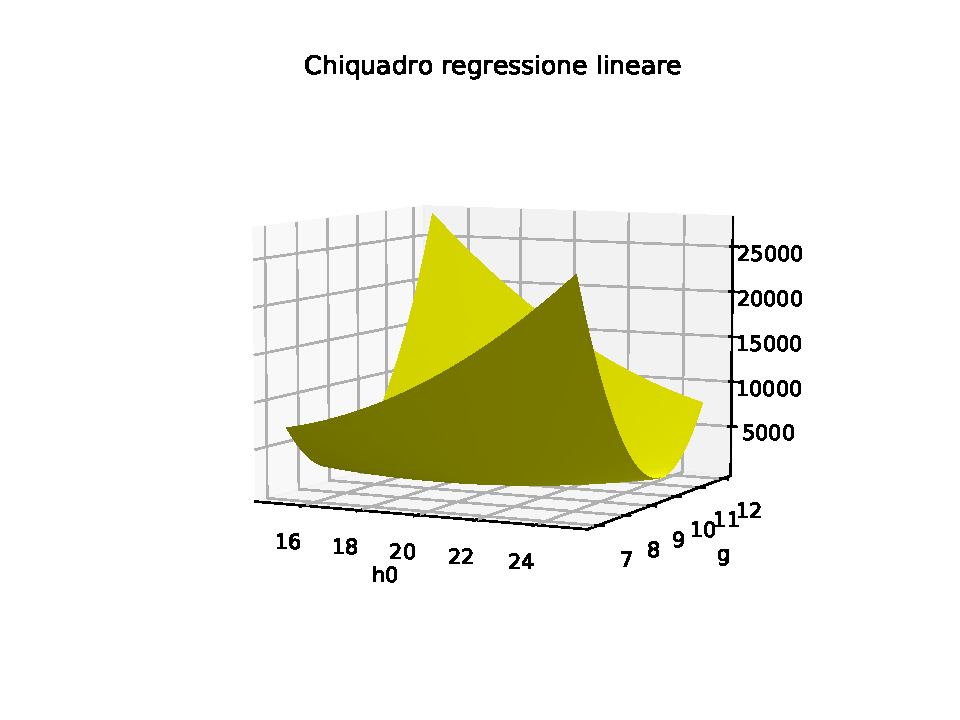
\includegraphics[scale=0.8]{img/chi_lin.pdf}
\caption{modello lineare $y(t)=h_0 - \frac{1}{2}gt^2$. Unico minimo, qualunque punto iniziale va bene.}
\end{figure}
\FloatBarrier
\FloatBarrier
\begin{figure}
\centering
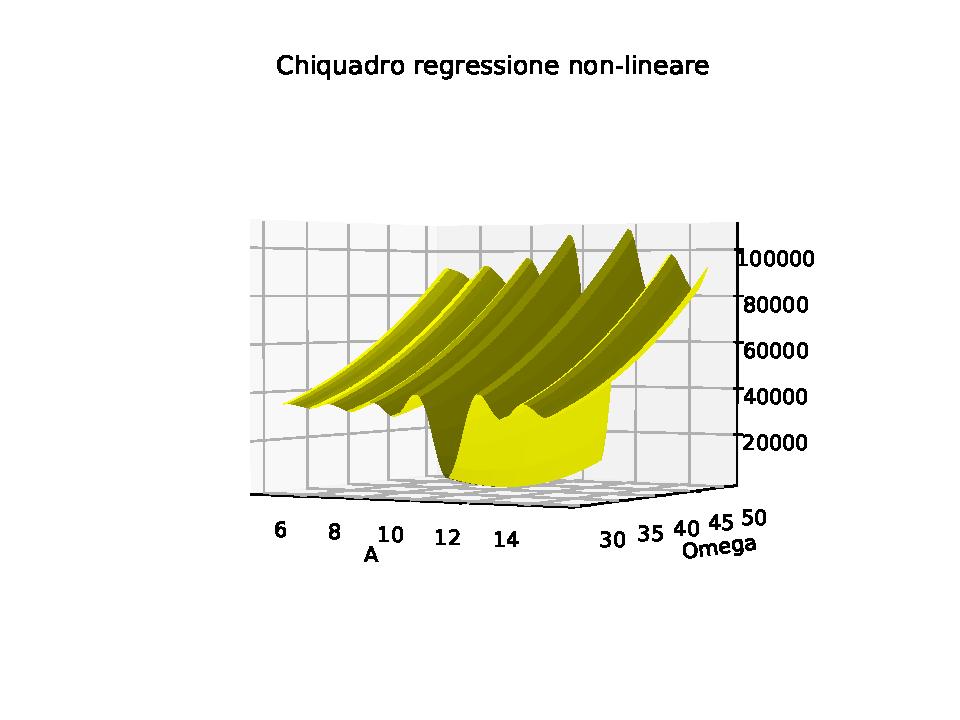
\includegraphics[scale=0.8]{img/chi_nlin.pdf}
\caption{modello non lineare $y(t)=Acos(\omega t)$. Tanti minimi locali bisogna stare attenti a dove partire altrimenti l'algoritmo si blocca su soluzioni non fisiche. Solo una piccola regione va bene come valori iniziali.}
\end{figure}
\FloatBarrier

I codici per generare i grafici che abbiamo visto non sono riportati per brevità ma sono presenti nella cartella.
Vediamo ora un semplice esempio di codice:

\begin{lstlisting}[language=Python]
import numpy as np
import matplotlib.pyplot as plt
from scipy.optimize import curve_fit

def Legge_oraria(t, h0, g):
    """
    Restituisce la legge oraria di caduta
    di un corpo che parte da altezza h0 e
    con una velocita' inziale nulla
    """
    return h0 - 0.5*g*t**2

""""
dati misurati:
xdata : fisicamemnte i tempi a cui osservo
        la caduta del corpo non affetti da
        errore
ydata : fisicamente la posizione del corpo
        misurata a dati tempi xdata afetta
        da errore
"""

#misuro 50 tempi tra 0 e 2 secondi
xdata = np.linspace(0, 2, 50)

#legge di caduta del corpo
y = Legge_oraria(xdata, 20, 9.81)
rng = np.random.default_rng()
y_noise = 0.3 * rng.normal(size=xdata.size)
#dati misurati afferri da errore
ydata = y + y_noise
dydata = np.array(ydata.size*[0.3])

#funzione che mi permette di vedere anche le barre d'errore
plt.errorbar(xdata, ydata, dydata, fmt='.', label='dati')

#array dei valori che mi aspetto, circa, di ottenere
init = np.array([15, 10])
#eseguo il fit
popt, pcov = curve_fit(Legge_oraria, xdata, ydata, init, sigma=dydata, absolute_sigma=False)

h0, g = popt
dh0, dg = np.sqrt(pcov.diagonal())
print(f'Altezza inziale h0 = {h0:.3f} +- {dh0:.3f}')
print(f"Accelerazione di gravita' g = {g:.3f} +- {dg:.3f}")

#garfico del fit
t = np.linspace(np.min(xdata), np.max(xdata), 1000)
plt.plot(t, Legge_oraria(t, *popt), label='fit')

plt.grid()
plt.title('Fit caduta grave', fontsize=15)
plt.xlabel('y(t) [m]', fontsize=15)
plt.ylabel('t [s]', fontsize=15)
plt.legend(loc='best')
plt.show()

[Output]
Altezza inziale h0 = 19.988 +- 0.065
Accelerazione di gravita' g = 9.790 +- 0.071
\end{lstlisting}

\begin{center}
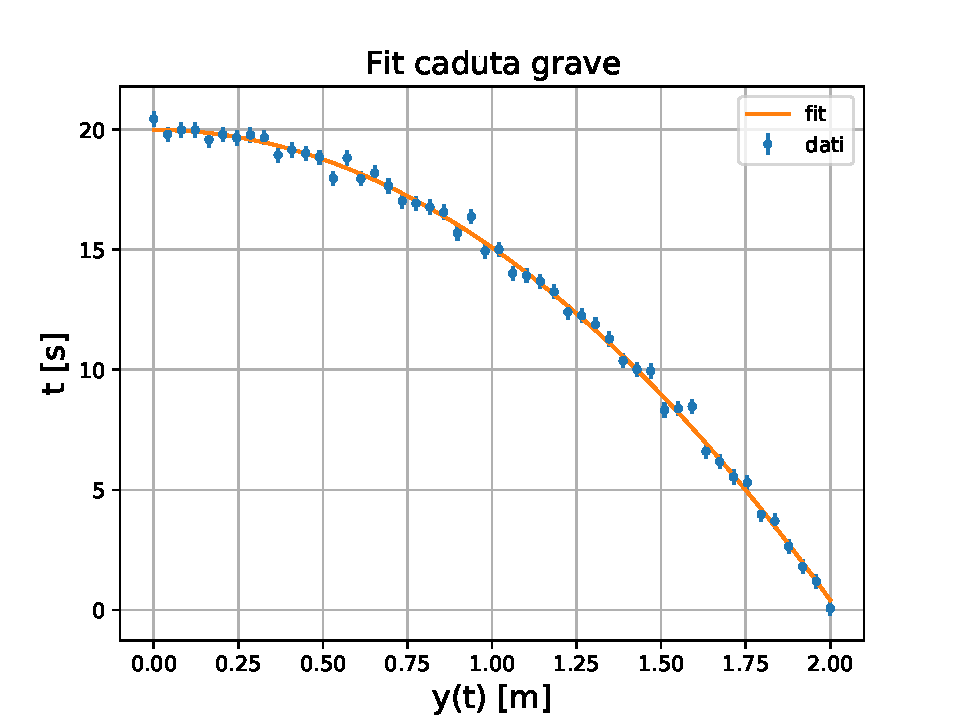
\includegraphics[scale=0.8]{img/fit_lez.pdf}
\end{center}
L'utilizzo dell'array init ci aiuta a trovare il minimo assoluto in modo che il codice vada a cercare intorno a quei valori, evitando che il codice si incastri altrove; anche se in questo caso non era necessario in quanto regressione lineare, è comunque buona norma utilizzarlo. Provate a fittare il modello non lineare visto sopra e vi accorgerete come solo una piccola regione dei parametri conduca alla soluzione corretta e che basti spostarvi di poco per ottenere risultati poco sensati. 
\subsubsection{Init}
Spero che abbiate capito, arrivati a questo punto, che è fondamentale mettere dei parametri iniziali sensati. Ma la domanda che sorge è come li determiniamo? Un po' come volete. Si possono fare tante cose, a seconda di che tipo di dati avete poi e da che processo fisico essi derivano. Io qui voglio solo fornirvi un piccolo codice che usando delle particolarità (i widget) di matplotlib permette di scrivere in un box la funzione che volete plottare, in codice python ovviamente, e dopo aver premuto invio essa viene plottata sui dati, in modo che voi abbiate sempre il grafico sottocchio (senza ogni volta chiudere il grafico, cambiare valori, ed eseguire di nuovo il codice).
\begin{lstlisting}[language=Python]
"""
Codice Per plottare i dati con una funzione per capire
i valori dei parametri ottimali da passare a curve_fit
"""

import numpy as np
import matplotlib.pyplot as plt
from matplotlib.widgets import TextBox

# Leggo i dati
#x_data, y_data, dy_data = np.loadtxt('...', unpack=True)

# Qui per comodita' li simulo
x_data  = np.linspace(0, 10, 60)
y_data  = 10*np.cos(2.5*x_data + np.pi/4) + 3

# Un po' di rumore quanto basta
rng = np.random.default_rng(seed=69420)
dy      = 1
y_noise = dy * rng.normal(size=x_data.size)
y_data +=  y_noise
dy_data = np.array(x_data.size*[dy])

# Creazione della figura
plt.figure(figsize=(8, 8))
plt.title("TITOLO")
plt.xlabel("t", fontsize=15)
plt.ylabel("F(t)", fontsize=15)
plt.subplots_adjust(bottom=0.2)
plt.errorbar(x_data, y_data, dy_data, c='k', fmt='.', label='data')

# Testo da scrivere inizialemente sulla barra per spiegare
text = "Insert here function, e.g. np.cos(t) or 3*t - 2 then press enter"

# Linspace per il plot e definiamo la variabile l che e' l'output del grafico
# ci servira' in quanto noi andremo a sovrascrivere questa variabile in modo
# che sia sempre tutto associato a questo grafico. Di default si plotta una
# retta alla media dei dati
t  = np.linspace(np.min(x_data), np.max(x_data), 1000)
l, = plt.plot(t, np.mean(y_data)*np.ones(t.size), 'b', label='fit law')
plt.legend(loc='best')
plt.grid()

def submit(text):
    '''
    Funzione che valuta l'espressione e la plotta

    Parameter
    ---------
    text : string
        Espressione da valutare scritta in python
    '''
    ydata = eval(text) # valuto l'espressione
    l.set_ydata(ydata) # aggiorno la variabile del plot
    plt.draw()         # Disegno il plot aggiornato

# Box per prendere l'input
axbox = plt.axes([0.15, 0.05, 0.75, 0.075])
text_box = TextBox(axbox, 'F(t)=', initial=text)
text_box.on_submit(submit)

plt.show()
\end{lstlisting}
\newpage

\subsection{Dietro curve fit: Levenberg-Marquardt}
Vogliamo ora provare ad andare dietro la libreria e vedere cosa fa effettivamente curve fit. Chiaramente i metodi di fit implementati sono molti e diversi, a seconda delle esigenze; per semplicità perciò andiamo a vedere quello che viene usato di default: Levenberg-Marquardt. Questo è un metodo iterativo, il che spiega la sensibilità ai valori iniziali, caratteristica di ogni metodo iterativo. Consideriamo la nostra funzione di fit $f$ la quale dipende da una variabile indipendente e da un insieme di parametri $\theta$, il quale fondamentalmente è un vettore di $\mathbb{R}^m$. Possiamo espandere $f$ in serie di taylor intorno ad un valore dei nostri parametri:
\begin{equation}
f (x_i, \theta_j + \delta_j ) \simeq f(x_i, \theta_j) + J_{ij} \delta_j
\end{equation}
dove $\delta_j$ è lo spostamento che vine fatto ad ogni passo dell'iterazione e $J_{ij}$ è il gradiente di f, o jacobinao se volete:
\begin{equation}
J_{ij} = \frac{\partial f(x_i, \theta_j)}{\partial \theta_j} = 
\begin{bmatrix} \dfrac{\partial f(x_1, \theta_1)}{\partial \theta_1} & \cdots & \dfrac{\partial f(x_1, \theta_m)}{\partial \theta_m} \\ \vdots & \ddots & \vdots \\ \dfrac{\partial f(x_n, \theta_1)}{\partial \theta_1} & \cdots & \dfrac{\partial f(x_n, \theta_m)}{\partial \theta_m}  \end{bmatrix}
\end{equation}
Che è una matrice $m \times n$ con $m<n$ altrimenti il metodo non funziona e dobbiamo adottare altre strategie. Per trovare il valore di $\delta$ espandiamo la (\ref{chisq}):
\begin{equation}
\begin{split}
S^2(\theta + \delta) &\simeq \sum_{i=1}^n \frac{(y_i - f (x_i, \beta) - J_{ij}\delta_j)^2}{\sigma_{y_i}^2} \\
&= (y - f(x, \theta) - J \delta)^{T} W (y - f(x, \theta) - J \delta)\\
&=(y - f(x, \theta))^{T} W (y - f(x, \theta)) - (y - f(x, \theta))^{T} W J \delta - (J \delta)^T W (y - f(x, \theta)) + (J \delta)^T W (J \delta) \\
&=(y - f(x, \theta))^{T} W (y - f(x, \theta)) - 2(y - f(x, \theta))^{T} W J \delta + \delta^T J^T W (J \delta)
\end{split}
\end{equation}
Dove $W$ è tale che $W_{ii} = 1/ \sigma_{y_i}^2$ e derivando rispetto a delta otteniamo il metodo di Gauss-Newton:
\begin{equation}
\frac{\partial S^2(\theta + \delta)}{\partial \delta} = - 2(y - f(x, \theta))^{T} W J + 2 \delta^T J^T W J=0
\end{equation}
per cui facendo il trasposto a tutto otteniamo:
\begin{equation}
(J^T W J) \delta = J^T W (y - f(x, \theta))
\end{equation}
La quale si risolve per $\delta$. Per migliorare la convergenza del metodo si introduce un parametro di damping $\lambda$ e l'equazione diventa:
\begin{equation}
(J^T W J - \lambda \, \text{diag}(J^T W J)) \delta = J^T W (y - f(x, \theta))
\end{equation}
Il valore di $\lambda$ viene cambiato a seconda se ci avviciniamo o meno alla soluzione giusta. Se ci stiamo avvicinando ne riduciamo il valore, andando verso il metodo di Gauss-Newton; mentre se ci allontaniamo ne aumentiamo il valore in modo che l'algoritmo si comporti più come un gradiente discendente (di cui in appendice ci sarà un esempio). La domanda è: come capiamo se ci stiamo avvicinando alla soluzione? Calcoliamo:
\begin{equation}
\begin{split}
\rho(\delta) &= \frac{S^2(x, \theta) - S^2(x, \theta + \delta)}{|(y - f(x, \theta) - J \delta)^{T} W (y - f(x, \theta) - J \delta)|} \\
& = \frac{S^2(x, \theta) - S^2(x, \theta + \delta)}{| \delta^T (\lambda \text{diag}(J^T W J) \delta + J^T W (y - f(x, \theta)))|}
\end{split}
\end{equation}
se $\rho(\delta) > \varepsilon_1$ la mossa è accetta e riduciamo $\lambda$ senno rimaniamo nella vecchia posizione.
Altra domanda a cui rispondere è: quando siamo arrivati a convergenza? definiamo:
\begin{align}
R1 &= \text{max}(|J^T W (y - f(x, \theta))|) \\
R2 &= \text{max}(| \delta/ \theta |) \\
R3 &= |S^2(x, \theta)/(n - m) - 1|
\end{align}
Se una di queste quantità è minore di una certa tolleranza allora l'algoritmo termina. Rimane ora un ultima domanda a cui rispondere e possiamo passare al codice. Dato che ci servono gli errori sui parametri di fit: come calcoliamo la matrice di covarianza? Basta calcolare:
\begin{equation}
\text{Cov} = (J^T W J)^{-1}
\end{equation}
quindi gli errori saranno semplicemente la radice degli elementi sulla diagonale, e le altre entrate le correlazioni fra parametri.\\
Passiamo ora al codice:

\begin{lstlisting}[language=Python]
"""
the code performs a linear and non linear regression
Levenberg-Marquardt algorithm. You have to choose
some parameters delicately to make the result make sense
"""

import numpy as np
import matplotlib.pyplot as plt


def lm_fit(func, x, y, x0, sigma=None, tol=1e-6, dense_output=False, absolute_sigma=False):
    """
    Implementation of Levenberg-Marquardt algorithm
    for non-linear least squares. This algorithm interpolates
    between the Gauss-Newton algorithm and the method of
    gradient descent. It is iterative optimization algorithms
    so finds only a local minimum. So you have to be careful
    about the values you pass in x0

    Parameters
    ----------
    f : callable
        fit function
    x : 1darray
        the independent variable where the data is measured.
    y : 1darray
        the dependent data, y <= f(x, {\theta})
    x0 : 1darray
        initial guess
    sigma : None or 1darray
        the uncertainty on y, if None sigma=np.ones(len(y)))
    tol : float
        required tollerance, the algorithm stop if one of this quantities
        R1 = np.max(abs(J.T @ W @ (y - func(x, *x0))))
        R2 = np.max(abs(d/x0))
        R3 = sum(((y - func(x, *x0))/dy)**2)/(N - M) - 1
        is smaller than tol
        
    dense_output : bool, optional dafult False
        if true all iteration are returned
    absolute_sigma : bool, optional dafult False
        If True, sigma is used in an absolute sense and
        the estimated parameter covariance pcov reflects
        these absolute values.
        pcov(absolute_sigma=False) = pcov(absolute_sigma=True) * chisq(popt)/(M-N)

    Returns
    -------
    x0 : 1d array or ndarray
        array solution
    pcov : 2darray
        The estimated covariance of popt
    iter : int
        number of iteration
    """

    iter = 0               #initialize iteration counter
    h = 1e-7               #increment for derivatives
    l = 1e-3               #damping factor
    f = 10                 #factor for update damping factor
    M = len(x0)            #number of variable
    N = len(x)             #number of data
    s = np.zeros(M)        #auxiliary array for derivatives
    J = np.zeros((N, M))   #gradient
    #some trashold
    eps_1 = 1e-1 
    eps_2 = tol
    eps_3 = tol
    eps_4 = tol

    if sigma is None :     #error on data
        W  = np.diag(1/np.ones(N))
        dy = np.ones(N)
    else :
        W  = np.diag(1/sigma**2)
        dy = sigma


    if dense_output:       #to store solution
        X = []
        X.append(x0)

    while True:
        #jacobian computation
        for i in range(M):                                  #loop over variables
            s[i] = 1                                        #we select one variable at a time
            dz1 = x0 + s*h                                  #step forward
            dz2 = x0 - s*h                                  #step backward
            J[:,i] = (func(x, *dz1) - func(x, *dz2))/(2*h)  #derivative along z's direction
            s[:] = 0                                        #reset to select the other variables

        JtJ = J.T @ W @ J                         #matrix multiplication, JtJ is an MxM matrix
        dia = np.eye(M)*np.diag(JtJ)              #dia_ii = JtJ_ii ; dia_ij = 0
        res = (y - func(x, *x0))                  #residuals
        b   = J.T @ W @ res                       #ordinate or dependent variable values of system
        d   = np.linalg.solve(JtJ + l*dia, b)     #system solution
        x_n = x0 + d                              #solution at new time

        # compute the metric
        chisq_v = sum((res/dy)**2)
        chisq_n = sum(((y - func(x, *x_n))/dy)**2)

        rho = chisq_v - chisq_n
        den = abs( d.T @ (l*np.diag(JtJ)@d + J.T @ W @ res))
        rho = rho/den
        # acceptance
        if rho > eps_1 :         #if i'm closer to the solution
            x0 = x_n             #update solution
            l /= f               #reduce damping factor
        else:
            l *= f               #else magnify

        # Convergence criteria
        R1 = np.max(abs(J.T @ W @ (y - func(x, *x0))))
        R2 = np.max(abs(d/x0))
        R3 = abs(sum(((y - func(x, *x0))/dy)**2)/(N - M) - 1)

        if R1 < eps_2 or R2 < eps_3 or R3 < eps_4:          #break condition
            break

        iter += 1

        if dense_output:
            X.append(x0)

    #compute covariance matrix
    pcov = np.linalg.inv(JtJ)

    if not absolute_sigma:
        s_sq = sum(((y - func(x, *x0))/dy)**2)/(N - M)
        pcov = pcov * s_sq

    if not dense_output:
        return x0, pcov, iter
    else :
        X = np.array(X)
        return X, pcov, iter
\end{lstlisting}
Il parametro dense\_output è stato inserito per fare un plot interessante per far vedere la dipendenza dalle condizioni iniziali.
Non riportiamo l'intero codice per non appesantire, la restante parte trattava solo di fare il plot delle curve di livello. In ogni caso è disponibile nell'apposita cartella il codice intero. Questo è il primo vero codice che fa qualcosa di molto complicato esso usa tutto quanto spiegato fin'ora e adesso è evidente l'importanza di mettere commenti, dare nomi sensati e rendere leggibile il codice. Bisogna ricordarsi che i codici in genere vengono scritti una volta ma letti tante volte quindi la chiarezza non va dosata con parsimonia.

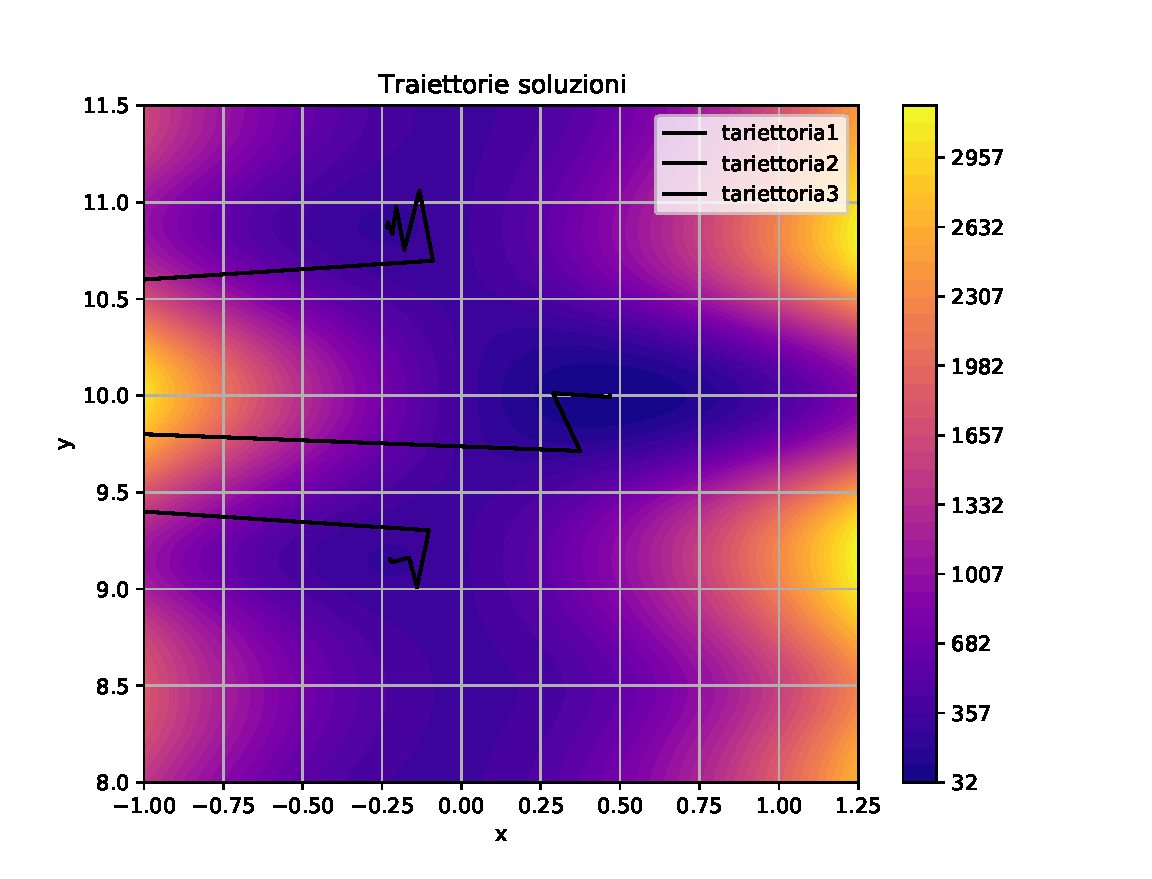
\includegraphics[scale=0.8]{img/traiettorie_fit.pdf}

Questo grafico rappresenta le curve di livello del modello non lineare $y(t) = A \cos( \omega t)$ ed è facile vedere come partendo da condizioni diverse il fit si incastri in minimo locali. L'asse y corrisponde a $\omega$ mentre l'asse x corrisponde ad $A$. Vediamo ora di testare i risultati del codice fittando qualcosa di un po' più bruttino. 

\begin{lstlisting}[language=Python]
"""
Test
"""
import numpy as np
import matplotlib.pyplot as plt
from scipy.optimize import curve_fit
from Lev_Maq import lm_fit


def f(t, A, o1, o2, f1, f2, v, tau):
    """fit function
    """
    return A*np.cos(t*o1 + f1)*np.cos(t*o2 + f2)*np.exp(-t/tau) + v

##data
x = np.linspace(0, 20, 1000)
y = f(x, 200, 10.5, 0.5, np.pi/2, np.pi/4, 42, 25)
rng = np.random.default_rng(seed=69420)
y_noise = 1 * rng.normal(size=x.size)
y  = y + y_noise
dy = np.array(y.size*[1])

##confronto

init = np.array([101, 10.5, 0.475, 1.5, 0.6, 35, 20])

pars1, covm1, iter = lm_fit(f, x, y, init, sigma=dy, tol=1e-8)
dpar1 = np.sqrt(covm1.diagonal())
pars2, covm2 = curve_fit(f, x, y, init, sigma=dy)
dpar2 = np.sqrt(covm2.diagonal())
print("        ------codice---------|--------scipy----------")
for i, p1, dp1, p2, dp2 in zip(range(len(init)), pars1, dpar1, pars2, dpar2):
    print(f"pars{i} = {p1:.5f} +- {dp1:.5f} ; {p2:.5f} +- {dp2:.5f}")

print(f"numero di iterazioni = {iter}")

chisq1 = sum(((y - f(x, *pars1))/dy)**2.)
chisq2 = sum(((y - f(x, *pars2))/dy)**2.)
ndof = len(y) - len(pars1)
print(f'chi quadro codice = {chisq1:.3f} ({ndof:d} dof)')
print(f'chi quadro numpy  = {chisq2:.3f} ({ndof:d} dof)')


c1 = np.zeros((len(pars1),len(pars1)))
c2 = np.zeros((len(pars1),len(pars1)))
#Calcoliamo le correlazioni e le inseriamo nella matrice:
for i in range(0, len(pars1)):
    for j in range(0, len(pars1)):
       c1[i][j] = (covm1[i][j])/(np.sqrt(covm1.diagonal()[i])*np.sqrt(covm1.diagonal()[j]))
       c2[i][j] = (covm2[i][j])/(np.sqrt(covm2.diagonal()[i])*np.sqrt(covm2.diagonal()[j]))
#print(c1) #matrice di correlazione
#print(c2)

##Plot
#Grafichiamo il risultato
fig1 = plt.figure(1)
#Parte superiore contenetnte il fit:
frame1=fig1.add_axes((.1,.35,.8,.6))
#frame1=fig1.add_axes((trasla lateralmente, trasla verticamente, larghezza, altezza))
frame1.set_title('Fit dati simulati',fontsize=15)
plt.ylabel('y [u.a.]',fontsize=15)
plt.grid()


plt.errorbar(x, y, dy, fmt='.', color='black', label='dati') #grafico i punti
t = np.linspace(np.min(x), np.max(x), 10000)
plt.plot(t, f(t, *pars1), color='blue', alpha=0.5, label='best fit codice') #grafico del best fit
plt.plot(t, f(t, *pars2), color='red' , alpha=0.5, label='best fit scipy') #grafico del best fit scipy
plt.legend(loc='best')#inserisce la legenda nel posto migliorte

#Parte inferiore contenente i residui
frame2=fig1.add_axes((.1,.1,.8,.2))

#Calcolo i residui normalizzari
ff1 = (y - f(x, *pars1))/dy
ff2 = (y - f(x, *pars2))/dy
frame2.set_ylabel('Residui Normalizzati')
plt.xlabel('x [u.a.]',fontsize=15)

plt.plot(t, 0*t, color='red', linestyle='--', alpha=0.5) #grafico la retta costantemente zero
plt.plot(x, ff1, '.', color='blue') #grafico i residui normalizzati
plt.plot(x, ff2, '.', color='red') #grafico i residui normalizzati scipy
plt.grid()
plt.show()

[Output]
        ------codice---------|--------scipy----------
pars0 = 199.85504 +- 0.17712 ; 199.85504 +- 0.17712
pars1 = 10.50005 +- 0.00009 ; 10.50005 +- 0.00009
pars2 = 0.49990 +- 0.00008 ; 0.49990 +- 0.00008
pars3 = 1.57040 +- 0.00087 ; 1.57040 +- 0.00087
pars4 = 0.78579 +- 0.00067 ; 0.78579 +- 0.00067
pars5 = 41.92350 +- 0.03125 ; 41.92350 +- 0.03125
pars6 = 24.99194 +- 0.05652 ; 24.99194 +- 0.05652
numero di iterazioni = 6
chi quadro codice = 969.017 (993 dof)
chi quadro numpy  = 969.017 (993 dof)
\end{lstlisting}
Non abbiamo stampato la matrice di covarianza per avere un po' più di ordine. Vediamo che tra i due non ci sono differenze, siamo felici. Vediamo anche il grafico:


\begin{center}
\makebox[\textwidth][c]{
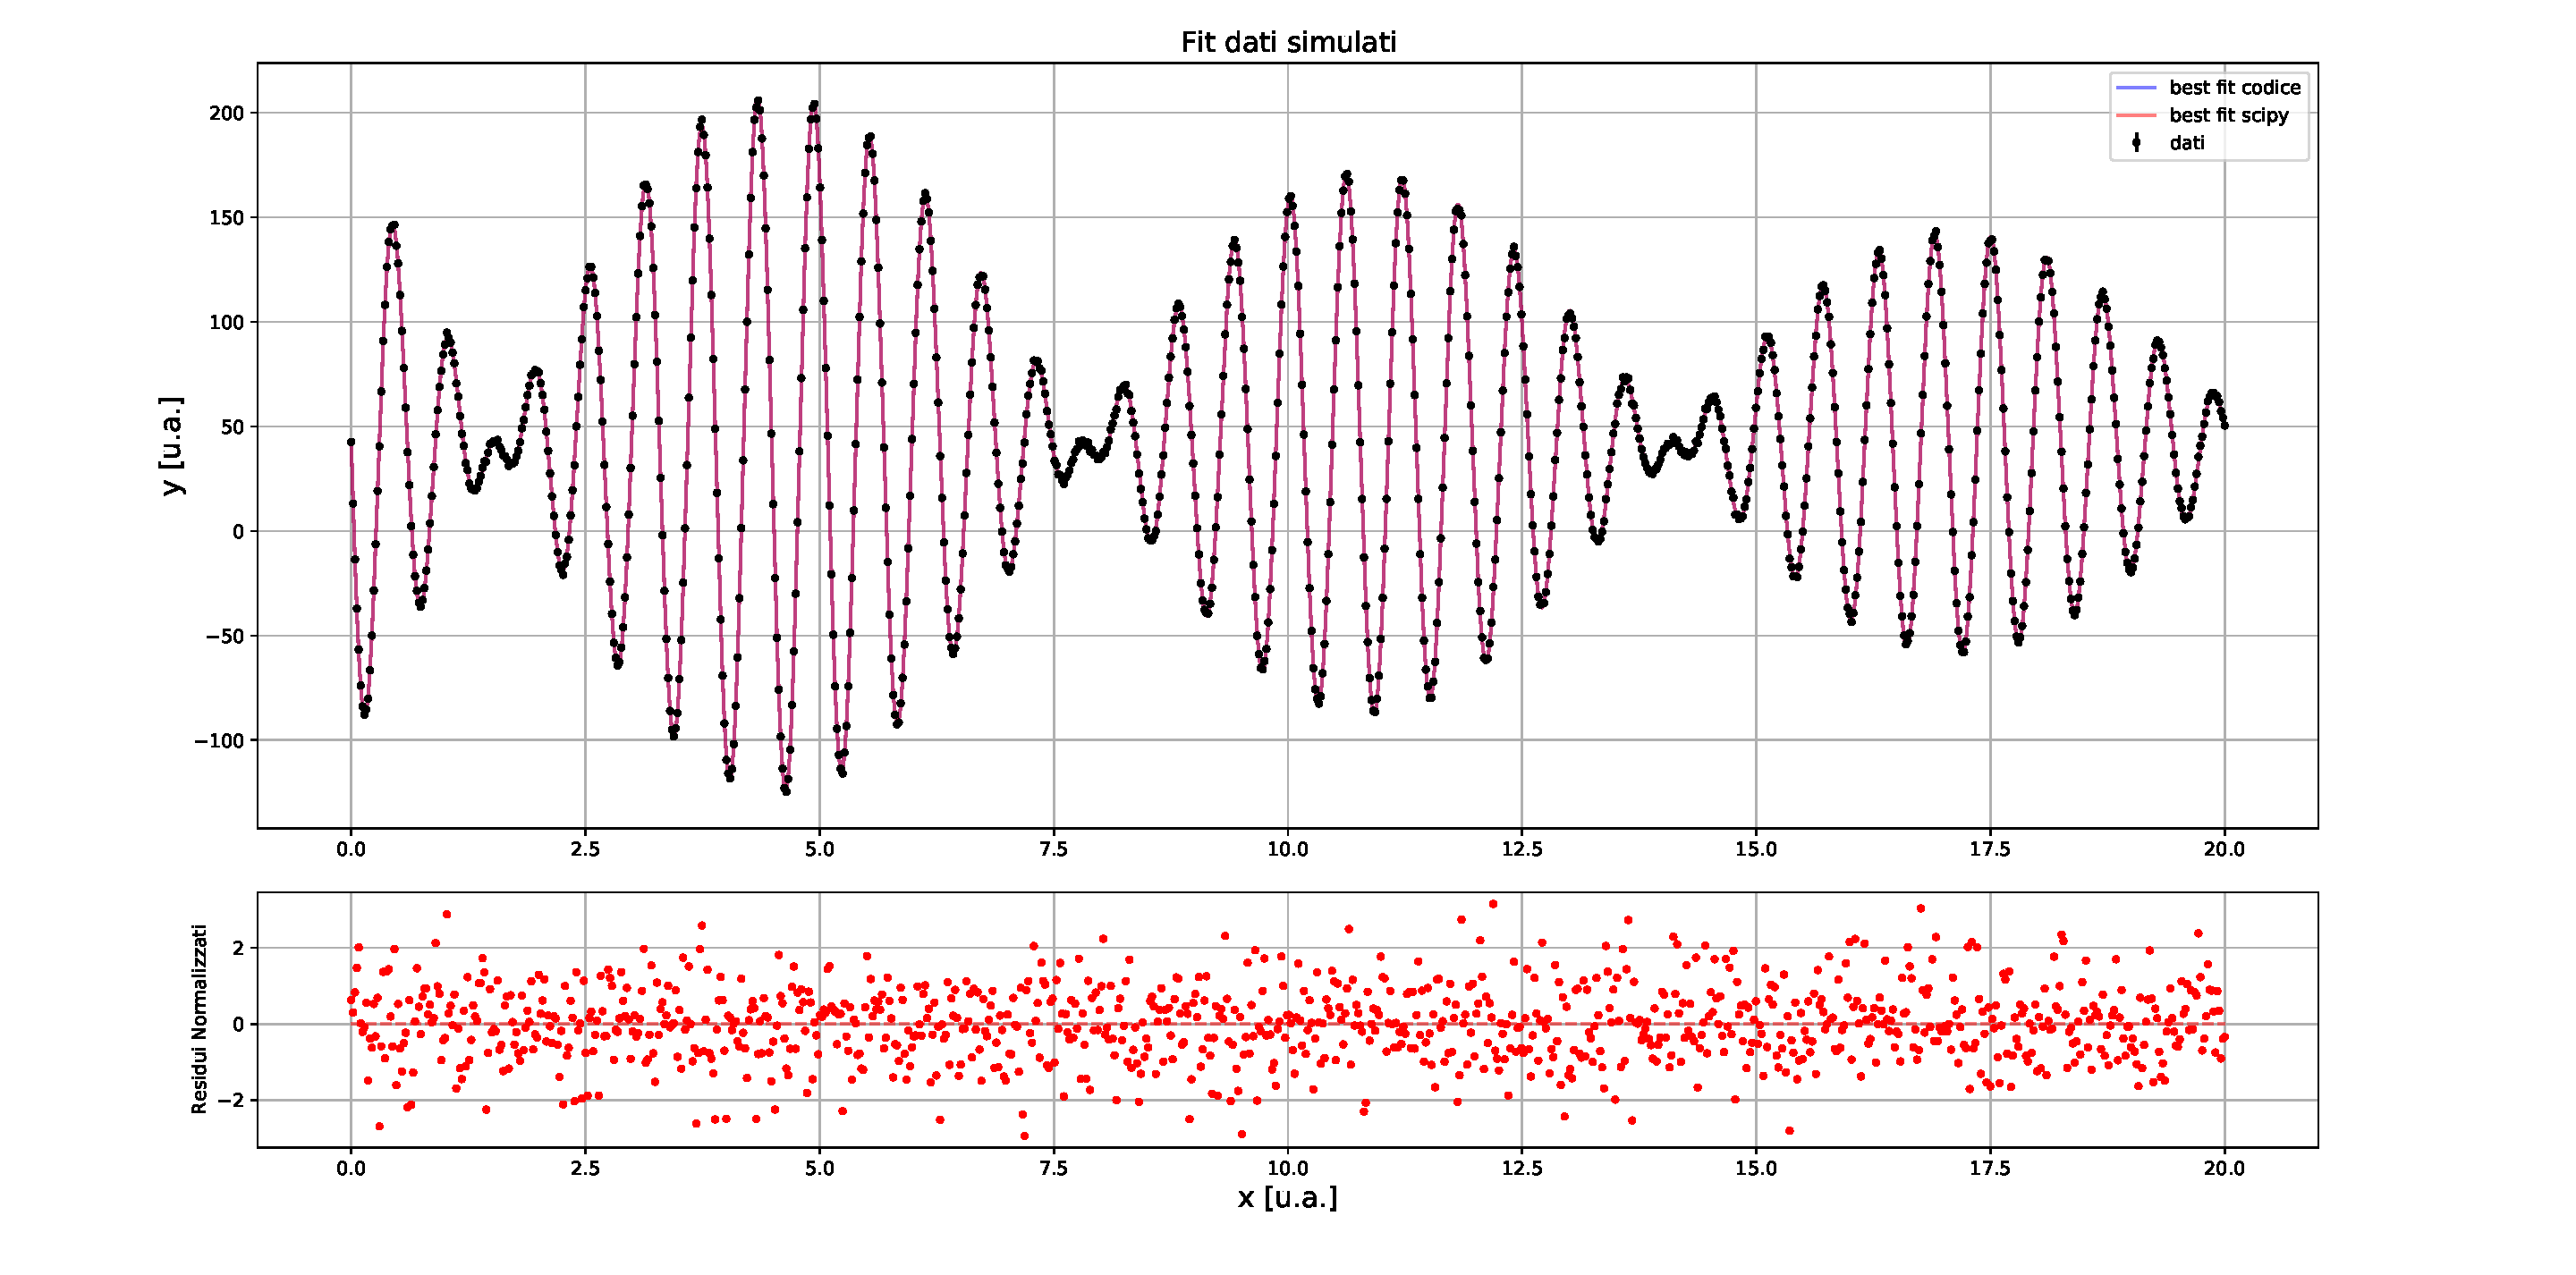
\includegraphics[scale=0.4]{img/test_fit.pdf}
}
\end{center}


\newpage
\section{Lezione Bonus: Version control}
Ok che le lezioni dovrebbero essere 4, ma come avete potuto vedere dall'indice ci sono una serie svariata di appendici e quindi tanto vale aggiungere questa lezione bonus che potrebbe essere molto utile. Tra l'altro potete capire da quanto appena scritto che questa sezione è stata aggiunta molto dopo. Non sappiamo nemmeno se sarà effettivamente una lezione che verrà tenuta. Però nella convinzione che possa essere utile io comunque provo a spiegarvelo. Come sapete queste note e i vari codici sono disponibili su un sito internet chiamato GitHub. GitHub è un sito che serve proprio per queste tipo di cose e per interagirci si può usare git o più semplicemente l'applicazione github desktop. Spieghiamo ora brevemente cos'è il controllo versione. Fondamentalmente immaginate di dover lavorare con più persone ad un progetto, che sia un codice software o una relazione di laboratorio. Quindi è necessario che tutti abbiano le stesse informazioni sui più recenti sviluppi fatti. Per quanto riguarda lo scrivere le relazione e basta magari uno può dire che esistono modi per scrivere e condividere il sorgente, ad esempio overleaf; ma non c'è solo la relazione, c'è anche il codice di analisi dati che sarebbe giusto tutti abbiano. Quindi quello che facciamo è creare un luogo remoto, ad esempio una repository su GitHub, in cui sarà caricato il codice e tutte le altre informazioni. Ogni membro potrà quindi farne una copia, tramite Git o github desktop, sul suo pc, quindi una copia locale della repository, che potrà modificare all'occorrenza. Tale copia si fa con il comando "\textbf{git clone} ..." vedremo poi il perché dei tre puntini. Una volta fatta le varie modifiche voi potete, allo stesso modo con cui avete scaricato la versione originale, potete caricarla dalla vostra repository locale sulla repository in remoto sul server. Vediamo un semplice schemino per rendere chiare le idee.

\begin{figure}[h]
\centering
\begin{tikzpicture}[>=latex]
%\draw[help lines] (0, 0) grid (15, 15);
%==================== Server in remoto ==================
\coordinate (A) at (6,13);
\coordinate (B) at (6,15);
\coordinate (C) at (9,15);
\coordinate (D) at (9,13);
\draw (A) to[out=0, in=180] (D);
\draw (A) to[out=90, in=270] (B);
\draw (B) to[out=0, in=180] (C);
\draw (D) to[out=90, in=270] (C);
\node at (7.5,14) {Server remoto};
%==================== Server locale 1 ==================
\coordinate (A) at (6,9);
\coordinate (B) at (6,11);
\coordinate (C) at (9,11);
\coordinate (D) at (9,9);
\draw (A) to[out=0, in=180] (D);
\draw (A) to[out=90, in=270] (B);
\draw (B) to[out=0, in=180] (C);
\draw (D) to[out=90, in=270] (C);
\node at (7.5,10.5) {Copia locale};
\node at (7.5,9.3) {pc};
%==================== Server locale 2 ==================
\coordinate (A) at (1,9);
\coordinate (B) at (1,11);
\coordinate (C) at (4,11);
\coordinate (D) at (4,9);
\draw (A) to[out=0, in=180] (D);
\draw (A) to[out=90, in=270] (B);
\draw (B) to[out=0, in=180] (C);
\draw (D) to[out=90, in=270] (C);
\node at (2.5,10.5) {Copia locale};
\node at (2.5,9.3) {pc};
%==================== Server locale 3 ==================
\coordinate (A) at (11,9);
\coordinate (B) at (11,11);
\coordinate (C) at (14,11);
\coordinate (D) at (14,9);
\draw (A) to[out=0, in=180] (D);
\draw (A) to[out=90, in=270] (B);
\draw (B) to[out=0, in=180] (C);
\draw (D) to[out=90, in=270] (C);
\node at (12.5,10.5) {Copia locale};
\node at (12.5,9.3) {pc};
%=================== Frecce =================================
\draw [->, line width=3pt, blue] (6,14.3) -- (2.2,11);
\draw [->, line width=3pt, blue] (9,14.3) -- (12.8,11);
\draw [->, line width=3pt, blue] (7.2,13) -- (7.2,11);
%=======================
\draw [<-, line width=3pt, red] (6,13.7) -- (2.8,11);
\draw [<-, line width=3pt, red] (9,13.7) -- (12.2,11);
\draw [<-, line width=3pt, red] (7.8,13) -- (7.8,11);
%=======================
\draw [->, line width=1pt, black] (7.5,9.6) -- (7.5,10.4);
\draw [->, line width=1pt, black] (2.5,9.6) -- (2.5,10.4);
\draw [->, line width=1pt, black] (12.5,9.6) -- (12.5,10.4);
%======================= Labels =============================
\node[rotate=42] at (4,13) {pull};
\node[rotate=42] at (4.6,12.2) {push};
\node[rotate=0] at (6.7,12) {pull};
\node[rotate=0] at (8.3,12) {push};
\node[rotate=360-42] at (11,13) {pull};
\node[rotate=360-42] at (10.4,12.2) {push};
\node[rotate=0] at (8.2,10) {commit};
\node[rotate=0] at (3.2,10) {commit};
\node[rotate=0] at (13.2,10) {commit};
\node[rotate=0] at (7,10) {add};
\node[rotate=0] at (2,10) {add};
\node[rotate=0] at (12,10) {add};
\end{tikzpicture}
\caption{Schema controllo versione distribuito.}
\end{figure}
I nomi che vedete accanto alle frecce sono i nomi delle operazioni, banalmente i comandi da dare a git. Spieghiamo un attimo: avete un certo file e lo modificate; dovete quindi aggiornare il vostro repositoy locale facendo "\textbf{git add nomefile.estensione}" e "\textbf{git commit nomefile.estensione}" (su github desktop vi basterà premere il tasto commit). Fatto ciò per spedire la copia in remoto vi basterà fare "\textbf{git push}". Se invece la copia locale è indietro rispetto alla copia remota, per aggiornare vi basterà fare "\textbf{git pull}". Ovviamente tutti questi comandi vanno scritti su shell, su github desktop vi basta preme i bottoni in cui ci sta scritto push, pull o che altro sia; abbastanza semplice. Buona norma è aggiungere un commento quando si fa il commit; commento che sarà visibile sulla repository locale. da shell basta fare "\textbf{git commit nomefile.estensione -m "commento da inserire"} ". Ciò è importante per far capire cosa avete fatto; infatti questo sistema di collaborazione tiene traccia di tutte le versioni di ciò su cui state lavorando, come una vera e propria cronologia, in modo che sia semplice risalire a vecchie versioni in caso di errori. Ora in linea di principio anche dentro il server remoto possono succedere cose, tra \textbf{fork}, \textbf{pull request}, \textbf{issue} e \textbf{merge}. Spieghiamo brevemente di che si tratta: Sia A la repository sull'account GitHub di persona A (ho molta fantasia). Voi potete premere dove ci sta scritto \textbf{fork} e creare così una copia della repository sul vostro account e fare tutto come detto sopra, creando un ramo secondario. Una volta fatto tutto potete fare una \textbf{pull request} cioè chiedere che la vostra modifica entri nel ramo principale dalla quale avete eseguito il \textbf{fork}; se chi gestice la repository (persona A) è d'accordo allora lui farà il \textbf{merge}. Tutto ciò può anche essere fatto su una vostra repository ovviamente. Infine un \textbf{issue} è una cosa che voi su GitHub aprite dicendo al mondo: sta cosa non funge. Tutto ciò nella speranza che qualcuno veda il vostro problema e attraverso tutti i meccanismi di sopra, o semplicemente con un commento vi aiuti a risolverlo o vi dia consigli sul da farsi.
Veniamo all'ultima questione lasciata in sospeso: "\textbf{git clone} ..." cosa ci va al posto dei tre puntini? Potete fare due cose: potete banalmente mettere l'HTTPS, prendendo l'url, ma lo trovate anche nella repository su GitHub premendo dove c'è un bottone verde con scritto "Code". Lì trovate anche l'SSH, altra cosa che potete utilizare, secondo me più comodo perché una volta che configurate l'SSH dopo aver creato il vostro acconut GitHub potrete fare tutto quello che volete senza che git vi chieda varie ed eventuali password. Per configurare la chiave SSH potete seguire i due link nell'ordine: prima lui \url{https://docs.github.com/en/authentication/connecting-to-github-with-ssh/generating-a-new-ssh-key-and-adding-it-to-the-ssh-agent} e poi lui \url{https://docs.github.com/en/authentication/connecting-to-github-with-ssh/adding-a-new-ssh-key-to-your-github-account}. \\
Con github desktop non avrete questi problemi nel clone e nel resto.


\newpage

\section{Prima Lezione A}
Uno dei problemi che spesso capita di dover affrontare in fisica è di dover diagonalizzare una matrice cioè trovare $\lambda$ e $\textbf{v}$ tale che:
\begin{equation}
A \textbf{v} = \lambda \textbf{v} \quad.
\end{equation}
A volte siamo interessati a tutti gli autovalori, a volte solo ai più grandi o a i più piccoli, dipende un po' dai casi, quindi vogliamo un po' far vedere qualche metodo per calcolare la decomposizione spettrale di una data matrice.
\subsection{Metodo delle potenze}
Il più semplice metodo da poter implementare è il metodo delle potenze, il quale è un algoritmo iterativo la cui regola di iterazione è:
\begin{equation}
\textbf{v}_{k+1} = \frac{A \textbf{v}_k}{|| A \textbf{v}_k ||} = \frac{A^k \textbf{v}_0}{|| A^k \textbf{v}_0 ||} \quad.
\end{equation}
Dove $\textbf{v}_0$ è un certo vettore iniziale che scegliamo a caso.
L'idea è abbastanza semplice, se $A$ è diagonalizzabile allora possiamo decomporre un vettore generico nella base degli autovettori di $A$:
\begin{equation}
\textbf{v}_0 = \alpha_1 \upsilon_1 + \cdots + \alpha_n \upsilon_n  \quad,
\end{equation}
Quindi applicando la potenza ennesima di $A$ a $v_0$ si ottiene:
\begin{align}
A^{k} \textbf{v}_0 &= \alpha_1 A^k \upsilon_1 + \cdots + \alpha_n A^k v_n \\
&= \alpha_1 \lambda_1^k v_1 + \cdots + \alpha_n \lambda_n^k v_n \\
&= \lambda_1^k \bigg( \alpha_1 v_1 + \cdots + \alpha_n \bigg(\frac{\lambda_n}{\lambda_1}\bigg)^k \upsilon_n \bigg) \quad.	
\end{align}
Quindi se gli autovalori sono tutti diversi e sono ordinati in ordine decrescente $\lambda_1 > \cdots > \lambda_n$ allora tutti i termini dentro la parentesi tendono a zero per $k$ che va all'infinito in quanto minori di uno. Questo metodo converge all'autovalore maggiore della matrice. Se volessimo trovarli tutti possiamo sempre usare questo metodo ma integrarlo con un metodo di ortogonalizzazione ad esempio Gram–Schmidt che chiamiamo ad ogni passo. Come criteri di convergenza possiamo mettere o la distanza tra iterazione successive dell'autovettore oppure la radice del valore assoluto della differenza tra iterazione successive dell'autovalore. Usiamo la radice perché la convergenza è quadratica negli autovalori:
\begin{equation}
\begin{split}
R_{1, 2} &= ||\textbf{v}_{k+1} \pm \textbf{v}_k || \\
R_3 &= \sqrt{|\lambda_{k+1} - \lambda_k|} \quad,
\end{split}
\end{equation}
dove il $\pm$ deriva dal fatto che sia $+ \textbf{v}$ che $-\textbf{v}$ sono autovettori. Quindi quando una di queste quantità è minore di una certa tolleranza che scegliamo noi l'algoritmo termina.\\
Capita sovente però che magari non si sia interessati a tutti gli autovalori, magari solo ai più grandi o a i più piccoli. Per i più grandi possiamo applicare l'algoritmo così come lo abbiamo descritto. Ma se fossimo interessati ai più piccoli? Per questo secondo basta sostituire $A$ con la sua inversa in quanto gli autovalori di $A^{-1}$ sono il reciproco degli autovalori di $A$ quindi il più grande autovalore di $A^{-1}$ sarà il più piccolo di $A$, proprio come volevamo; questo si chiama metodo delle potenze inverso. In genere questo in questo metodo non si inverte direttamente $A$; si usa invece una routine per risolvere un sistema. Qui è stato deciso invece di invertire direttamente la matrice di partenza senza farci troppi problemi. Vediamo ora il codice:

\begin{lstlisting}[language=Python]
import numpy as np

def eig(M, k=None, tol=1e-10, magnitude='small'):
    '''
    Compute the eigenvalue decomposition
    of the symmetric matrix A using power iteration
    or inverse iteration.
    Inverse iteration is the same of power iteration
    but we use M^-1 instead of M so the eigenvalues
    are the reciprocal.

    Parameters
    ----------
    M : 2darray
        N x N matrix, symmetric
    k : None or int, if None k=N
        number of eigenvariates and eigenvectors to find,
        if k<N then k eigenvectors corresponding to the k
        largest eigenvalues will be found
    tol : float, optional default 1e-10
        required tollerance
    magnitude : string, optional, default small
        if magnitude == 'small' the smallest eigenvalues
        and thei relative eigenvectors will be computed
        if magnitude == 'big' the biggest eigenvalues
        and thei relative eigenvectors will be computed

    Return
    ------
    eigval : 1darray
        array of eigenvalues
    eigvec : 2darray
        kxk matrix, the column eigvec[:, i] is the
        ormalized eigenvector corresponding to the
        eigenvalue eigval[i]
    counts : 1darray
        how many iteration are made for each eigenvector
    '''

    if magnitude == 'small':
        A = np.copy(np.linalg.inv(M))
    if magnitude == 'big':
        A = np.copy(M)
        
    N = A.shape[0]
    if k is None:
        k = N

    eigvec = []  # will contain the eignvectors
    eigval = []  # will contain the eignvalues
    counts = []  # will contain the numbero of iteration of each eigenvalue

    for _ in range(k):

        v_p = np.random.randn(N) #initial vector
        v_p = v_p / np.sqrt(sum(v_p**2))
        l_v = np.random.random()
        Iter= 0

        while True:
            l_o = l_v
            v_o = v_p                          # update vector
            v_p = np.dot(A, v_p)               # compute new vector
            v_p /= np.sqrt(sum(v_p**2))        # normalization

            # Orthogonalization respect
            # all eigenvectors find previously
            for i in range(len(eigvec)):
                v_p = v_p - np.dot(eigvec[i], v_p) * eigvec[i]
                
            #eigenvalue of v_p, A @ v_p = l_v * v_p
            #multiplying by the transposed => (A @ v_p) @ v_p.T = l_v
            #using v_p @ v_p.T = 1
            l_v = np.dot(np.dot(A, v_p), v_p)
            
            R1 = np.sqrt(sum((v_p - v_o)**2))
            R2 = np.sqrt(sum((v_o + v_p)**2))
            R3 = np.sqrt(abs(l_v - l_o))      # In eigenvalues the convergence is quadratic

            Iter += 1
            if R1 < tol or R2 < tol or R3 < tol:
                break

        eigvec.append(v_p)
        eigval.append(l_v)
        counts.append(Iter)
    
    if magnitude == 'small':
        eigval = 1/np.array(eigval)
        eigvec = np.array(eigvec).T
    if magnitude == 'big':
        eigvec = np.array(eigvec).T
        eigval = np.array(eigval)

    return eigvec, eigval, counts
    
\end{lstlisting}

Vediamo ora i risultati due test del nostro algoritmo. Cominciamo generando una matrice random grazie a numpy e per averla simmetrica consideriamone il prodotto per se stessa trasposta: "P = np.random.normal(size=[n, n]) H = np.dot(P.T, P)"; quindi diagonalizziamo H, prendiamo $n=100$, settando "magnitude='big'". Mostriamo solo il risultato, il codice lo troverete scritto nella cartella, confrontando il risultato con la diagonalizzazione fatta da numpy:

\begin{center}
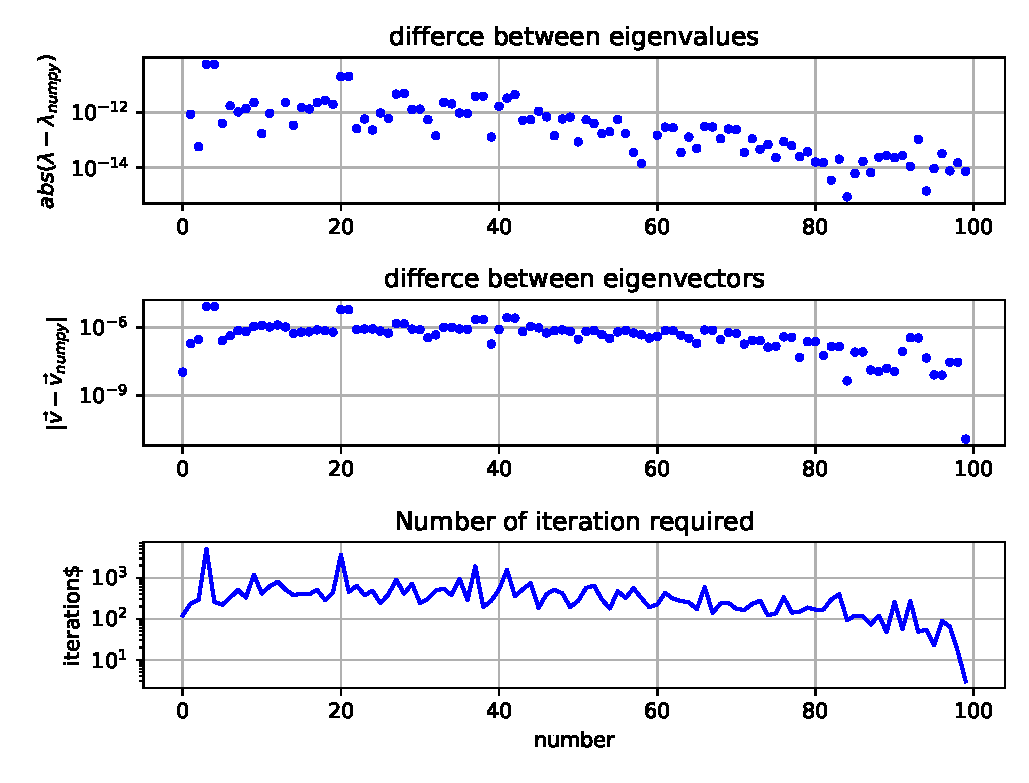
\includegraphics[scale=0.7]{img/cfr_eig.pdf}
\end{center}

Dal punto di vista del tempo chiaramente numpy nemmeno fa fatica: $14.240$ secondi noi contro $0.001$ di numpy, e ci guarda pure con aria di superiorità perché gli facciamo schifo. Comunque il risultato è soddisfacente.\\

\subsection{Equazione di Schrödinger}
Vediamo ora un test un po' più fisico dove siamo interessati agli autovalori più piccoli. Consideriamo una matrice 'a bischero' fatta del tipo:
\begin{equation}
H = - \frac{1}{2h^2}
\begin{pmatrix}
-2 & 1  & 0 & \cdots &0\\
1  & -2 & 1 & \cdots &0\\
0 & \ddots & \ddots & \ddots &\vdots \\
\vdots & \ddots & 1 &  -2 & 1 \\
0 & \cdots &0&  1 & -2 \\
\end{pmatrix}
+
\begin{pmatrix}
V(x_1) & 0  & 0 & \cdots &0\\
0  & V(x_2) & 0 & \cdots &0\\
0 & \ddots & \ddots & \ddots &\vdots \\
\vdots & \ddots & 0 &  V(x_{N-1}) & 0 \\
0 & \cdots &0&  0 & V(x_N) \\
\end{pmatrix}
\end{equation}
dove $h$ è la spaziatura tra $x_i$ e $x_{i+1}$ il quale è un array in un certo range in un certo numero di punti. Probabilmente avrete notato che la matrice scritta sopra non è altro che la discretizzazione dell'equazione di Schrödinger (non stiamo qui a ricavarla, lo vedrete nei corsi di meccanica quantistica, prendetela per buona per il momento) non dipendente dal tempo :
\begin{equation}
H \psi = \bigg( - \frac{1}{2}\frac{\partial^2}{\partial x^2} + V(x) \bigg) \psi = E \psi
\end{equation}
Qui chiaramente siamo interessati solo ai livelli energetici minori in quanto l'approssimazione del laplaciano che abbiamo fatto peggiora man mano che gli stati sono sempre più estesi, discretizzare così infatti significa mettersi dentro una scatola di lato fissato ma chiaramente noi vorremmo la scatola infinita, quindi per i livelli più bassi l'approssimazione è buona ($h = L/N$ nel nostro caso abbiamo preso L=20 e N=1000).
Per semplicità consideriamo il caso dell'oscillatore armonico $V(x) = x^2/2$ e troviamo i dieci autovalori più bassi (analiticamente e in unità naturali $E=n+1/2$). Grafichiamo anche poi per bellezza tre autovettori, o autofunzioni, con il caveat che ogni autovettore va diviso per $\sqrt{h}$. Come sopra il codice è già scritto e lo trovate tutto insieme, noi qui mostriamo solo i risultati:
\begin{center}
\begin{tabular}{ccc}
  \hline
  teorico &calcolato&errore \\
  \hline 
  0.5 & 0.50049 & 4.88e-04 \\ 
   
  1.5 & 1.50144 & 1.44e-03 \\ 
 
  2.5 & 2.50234 & 2.34e-03 \\ 
  
  3.5 & 3.50319 & 3.19e-03 \\ 
  
  4.5 & 4.50399 & 3.99e-03 \\ 
  
  5.5 & 5.50474 & 4.74e-03 \\ 

  6.5 & 6.50544 & 5.44e-03 \\ 

  7.5 & 7.50609 & 6.09e-03 \\ 

  8.5 & 8.50669 & 6.69e-03 \\ 

  9.5 & 9.50724 & 7.24e-03 \\ 
  \hline 
\end{tabular}   
\end{center}

\begin{center}
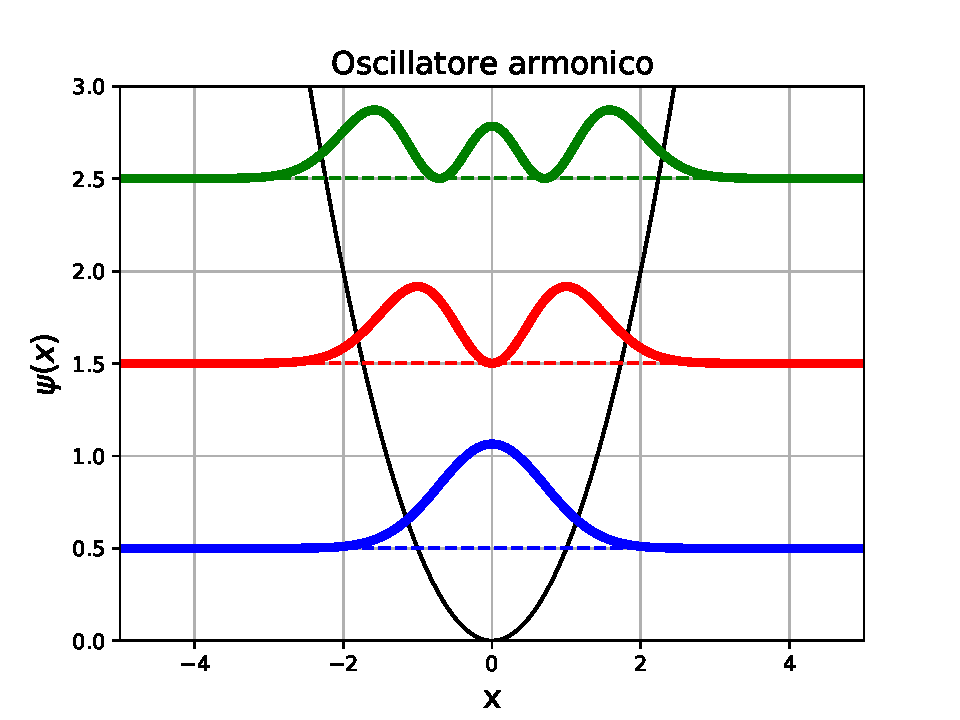
\includegraphics[scale=0.9]{img/mq.pdf}	 
\end{center}

Per un totale di tempo di esecuzione di $0.77814$ secondi. Precisiamo infine che benché essa sia un'equazione differenziale ordinaria non può essere risolta come tale in quanto non è noto a priori il valore dell'energia. Volendo si può adottare una strategia simile usando il metodo di shooting, ovvero si risolve l'equazione come fosse una normale ode usando una guess per l'energia e poi si usa l'energia come parametro di shooting; Si cerca quindi tramite un algoritmo di root finding un valore di $E$ (parametro di shooting) che dia un buon risultato (dove buono si intende che c'è una variazione di una qualche quantità minore di una tolleranza da noi settata). Un esempio di metodo di shooting, anche se non applicato all'equazione di Schrödinger è presente nelle appendici. 

\subsection{Algoritmo QR}
Vediamo adesso un altro algoritmo che può essere interessante trattare. Come si può intuire dal nome questo algoritmo si basa sulla scomposizione $QR$ di una matrice, dove $Q$ è una matrice ortogonale $Q^T = Q^{-1}$ e $R$ è una matrice triangolare superiore. Data quindi la nostra matrice $A$ da diagonalizzare quello che si fa è, chiamando $A_0=A=Q_0 R_0$:
\begin{equation}
A_{k+1} = R_k Q_k = Q^{-1}_k Q_k R_k Q_k = Q^T_k A_k Q_k \quad.
\end{equation}
Vedete quindi che procedendo per trasformazioni ortogonali tutte le $A_k$ sono simili. Avremo quindi che gli autovalori saranno gli elementi sulla diagonale della matrice $A_{k+1}$. Mentre per gli autovettori quello che si fa è calcolare il prodotto delle varie $Q_k$ con loro stesse:
\begin{equation}
V = Q_0 Q_1 \hdots Q_{k} \quad,
\end{equation}
$V$ sarà la matrice che conterrà gli autovettori di $A$. Tutto ciò viene eseguito un certo tot di volte che scegliamo noi da input. Per completare la spiegazione andiamo a vedere come si esegue la decomposizione $QR$.
Fondamentalmente si tratta di applicare Gram-Schmidt alle colonne di $A$.
\begin{equation}
A = [\textbf{a}_1 | \textbf{a}_2 | \hdots | \textbf{a}_N]
\end{equation}

\begin{align*}
\textbf{v}_1 & = \textbf{a}_1, & \textbf{e}_1 & = \frac{\mathbf{v}_1}{\|\mathbf{v}_1\|} \\
\mathbf{v}_2 & = \mathbf{a}_2 - (\mathbf{a}_2 \cdot \textbf{e}_1) \textbf{e}_1,
& \mathbf{e}_2 & = \frac{\mathbf{v}_2}{\|\mathbf{v}_2\|} \\
& {}\ \  \vdots & & {}\ \  \vdots \\
\mathbf{v}_k & = \mathbf{a}_k-\sum_{j=1}^{k-1} (\mathbf{a}_{k} \cdot \textbf{e}_j) \textbf{e}_j, & \mathbf{e}_k & = {\mathbf{u}_k\over \|\mathbf{u}_k \|}.
\end{align*}
Dunque possiamo arrivare a dire che:
\begin{equation}
A = [\textbf{e}_1 | \textbf{e}_2 | \hdots | \textbf{e}_N]
\begin{pmatrix}
\mathbf{a}_1 \cdot \textbf{e}_1 & \mathbf{a}_2 \cdot \textbf{e}_1 & \cdots & \mathbf{a}_N \cdot \textbf{e}_1 \\
0  & \mathbf{a}_2 \cdot \textbf{e}_2 & \cdots & \mathbf{a}_N \cdot \textbf{e}_2\\
\vdots & \vdots & \ddots & \vdots \\
0 & 0 & \cdots & \mathbf{a}_N \cdot \textbf{e}_N \\
\end{pmatrix}
= Q R \quad.
\end{equation}
Questo metodo, a differenza del precedente, con il quale potevamo scegliere quanti autovalori e autovettori farci calcolare, restituisce tutti gli autovalori e gli autovettori della nostra matrice. Siamo in Python, probabilmente per matrici grandi ci vorrà tanto.
Passiamo quindi adesso al codice:
\begin{lstlisting}[language=Python]
#=====================================================================
# Function to compute QR decomposition
#=====================================================================

def QR_decomp(A):
    '''
    Comupute QR decomposition of a matrix A
    
    Parameters
    ----------
    A : 2darray
        N x N matrix
    
    Returns
    -------
    Q, R : 2darray
        A = Q @ R
    '''
    
    # we give different names because in principle the QR
    # decomposition also applies to non-square matrices
    n, m = A.shape

    Q = np.zeros((n, n)) # Initialize matrix Q
    R = np.zeros((n, m)) # Initialize matrix R
    v = np.zeros((n, n)) # Initialize matrix v: for Gram-Schmidt

    u[:, 0] = A[:, 0]
    Q[:, 0] = v[:, 0] / np.sqrt(sum(v[:, 0]**2))

    for i in range(1, n):

        v[:, i] = A[:, i]
        for j in range(i):
            v[:, i] -= (A[:, i] @ Q[:, j]) * Q[:, j]

        Q[:, i] = v[:, i] / np.sqrt(sum(v[:, i]**2))

    
    for i in range(n):
        for j in range(i, m):
            R[i, j] = A[:, j] @ Q[:, i]
    
    # uncomment for scipy comparison      
    #D = np.diag(np.sign(np.diag(Q)))
    #Q[:, :] = Q @ D
    #R[:, :] = D @ R

    return Q, R

#=====================================================================
# Function to solve eigensystem via QR iterartion
#=====================================================================

def QR_eig(A, maxiter=100):
    '''
    Find the eigenvalues of A using QR iteration.
    
    Parameters
    ----------
    A : 2darray
        N x N matrix
    maxiter : int, optional, default 100
        number of iterations to do
    
    Returns
    -------
    eigval : 1darray
        array of eigenvalues
    eigvec : 2darray
        N x N matrix, the column eigvec[:, i] is the
        ormalized eigenvector corresponding to the
        eigenvalue eigval[i]
    '''
    A_new, A_old = [np.copy(A)]*2
   
    eigvec = np.eye(A.shape[0])
      
    for i in range(maxiter):
        
        A_old[:, :] = A_new
        Q, R = QR_decomp(A_old)

        A_new[:, :] = R @ Q
        eigvec = eigvec @ Q       

    eigval = np.diag(A_new)

    return eigval, eigvec
\end{lstlisting}
Facendo la prova con la stessa matrice a bischero di prima infatti otteniamo un tempo di 717.6 secondi, usando le iterazioni di default. I risultati sono gli stessi che quelli mostrati in precedenza. Attenzione ora però all'ordine degli autovalori, dovrebbero essere ordinati dal più grande al più piccolo.
\subsection{Lanczos}
Un'ultima cosa carina da spiegare è l'iterazione di Lanczos, caso particolare della più generale iterazione di Arnoldi; ma per i casi di interesse fisico le ipotesi sono sempre ragionevoli: la matrice da diagonalizzare deve essere hermitiana. L'idea è di trovare due matrici per cui valga:
\begin{equation}
A = Q^{\dagger} H Q .
\end{equation}
$H$ sarà un amatrice tridiagonale simmetrica reale e sarà quella che andremo a diagonalizzare. Essa sarà una matrice più piccola rispetto ad $A$, la dimensione è un parametro che scegliamo noi, quindi verrà più leggero il conto, ma non siamo in grado di recuperare tutti gli autovalori, e autovettori di $A$. L'unico modo per farlo è imporre che $H$ abbia la stessa dimensione di $A$. $Q$ invece sarà una certa matrice con colonne ortonormali; se poi $T$ ha la stessa dimensione di $A$ allora $Q$ sarà unitaria. Tornando a noi diagonalizzando $H$ avremo un certo numero di autovalori, che sono anche autovalori di $A$, non necessariamente tutti sequenziali. Per gli autovettori invece, se vale $H \textbf{y}= \lambda \textbf{y}$ allora $Q y$ è autovalore di $A$.
Vediamo subito il codice:
\begin{lstlisting}[language=Python]
def lanczos(A, n):
    '''
    Lanczos iteration for a matrix A
    
    Parameter
    ---------
    A : 2darray
        Hermitian N x N matrix
    n : int
        dimension of Krylov subspace
        e.g. dimension of H
    
    Return
    ------
    Q, H : 2darray
        A = Q.T H Q
    '''
    m     = A.shape[0]
    Q     = np.zeros((m, n+1))
    alpha = np.zeros(n)
    beta  = np.zeros(n)
    b     = np.random.randn(m)
    
    Q[:,0] = b/np.sqrt(sum(b**2))
    
    for i in range(n):
        v        = np.dot(A, Q[:,i])
        alpha[i] = np.dot(Q[:,i], v)
        
        if i == 0:
            v = v - alpha[i] * Q[:, i]
        else :
            v = v - beta[i-1] * Q[:, i-1] - alpha[i] * Q[:, i]
        
        beta[i]  = np.sqrt(sum(v**2))
        Q[:,i+1] = v / beta[i]
    
    H = Q.T @ A @ Q
    
    return Q, H
\end{lstlisting}
Calcolata $H$ la passiamo quindi a una delle funzioni sopra scritte e vediamo che succede. Per riuscire a prendere dei buoni risultati per i primi livelli eccitati usiamo come $n=300$, quindi l'algoritmo QR ora sarà un po' più spiccio. Vediamo cosa esce sempre per il caso dell'oscillatore armonico.
\begin{center}
\begin{tabular}{c|cc|cc}
  \hline
  teorico & QR & errore & potenze & errore \\
  \hline 
0.5 & 0.50068 & 6.80e-04 & 0.50068 & 6.80e-04\\
1.5 & 1.50146 & 1.46e-03 & 1.50145 & 1.45e-03\\
2.5 & 2.50321 & 3.21e-03 & 2.50257 & 2.57e-03\\
3.5 & 3.59515 & 9.51e-02 & 3.59459 & 9.46e-02\\
4.5 & 4.61829 & 1.18e-01 & 4.61261 & 1.13e-01\\
5.5 & 6.60135 & 1.10e+00 & 6.59104 & 1.09e+00\\
6.5 & 7.76801 & 1.27e+00 & 7.74208 & 1.24e+00\\
7.5 & 10.35934 & 2.86e+00 & 10.36662 & 2.87e+00\\
8.5 & 12.02403 & 3.52e+00 & 12.04071 & 3.54e+00\\
9.5 & 13.48530 & 3.99e+00 & 13.49227 & 3.99e+00\\
  \hline 
\end{tabular}   
\end{center}
Vedete quindi come per i primi 5 livelli vada tutto bene, poi gli altri autovalori sono diversi o un po' sbagliati: ad esempio 10.35 è un po' lontano mentre 13.49 è già un migliore risultato. Come dicevamo prima vedete poi che ci sono degli autovalori che sono spariti in quanto $H$ è solo $300 \times 300$. Dal punto di vista dei tempi QR impiega circa 48 secondi, mentre il metodo delle potenze circa 0.1 secondi. 


















\newpage


\section{Seconda lezione A}
\subsection{Trasformate di Fourier}
\subsubsection{DFT}
La trasformata di Fourier è una trasformata integrale che ci  permette di cambiare dominio della nostra funzione: ad esempio da tempo a frequenze o da spazio a numero d'onda. Data una funzione:
\begin{equation}
f(t) \quad \text{tale che} \quad \int_{-\infty}^{\infty} |f(t)| dt < \infty
\end{equation}
Definiamo trasformata e anti trasformata di $f$ come:
\begin{align}
\tilde{f}(\omega) &= \int_{-\infty}^{\infty} f(t) e^{-i \omega t} dt = \mathcal{F}\{ f \}(\omega) \\
f(t) &= \frac{1}{2 \pi} \int_{-\infty}^{\infty} \tilde{f}(\omega) e^{-i \omega t} d \omega =  \mathcal{F}^{-1}\{ \tilde{f} \}(t) \\
\end{align}
e gode di varie proprietà:
\begin{equation}
\mathcal{F}(D^k f) = (-i \omega)^k \mathcal{F}(f) \hspace{5 mm}
\mathcal{F}(f(t-a))=e^{i\omega a} \mathcal{F}(f(t)) \hspace{5 mm}
\mathcal{F}(e^{i\omega a}f(t)) = \tilde{f}(\omega - a) \hspace{5 mm}
\mathcal{F}((it)^k f)=D^{k} \mathcal{F}(f)
\end{equation}
Qui abbiamo in realtà aggiunto altre ipotesi su $f$ (e.g. $f \in C^{k}$) ma va beh.
Vediamo un piccolo grafico che meglio ci consenta di capire, in maniera intuitiva, cosa vuol dire questo cambio di base:
\FloatBarrier
\begin{figure}[h]
% Preamble:\pgfplotsset{width=7cm,compat=1.18}
\begin{tikzpicture}[>=latex]
\begin{axis}[xlabel=frequenze, ylabel=tempo,
    ymin=-5,ymax=15, xmin=0,xmax=1.2,
    extra x ticks={1,1.1},
    extra x tick style={grid=major},
    extra x tick labels={1, 1.1},
]  
    extra x tick style={xticklabel=(1, 1.07),}]
    \addplot3 [red, domain=-5:15, samples=200, samples y=1]
    (0, x, {(sin(2*3.1415*deg(x))+sin(2*3.1415*deg(x)*1.1))});
    \addplot3 [blue, domain=-5:15, samples=200, samples y=1]
    (1, x, {sin(2*3.1415*deg(x))});
    \addplot3 [green, domain=-5:15, samples=200, samples y=1]
    (1.1, x, {sin(2*3.1415*deg(x)*1.1)});
\end{axis}
\end{tikzpicture}
\begin{tikzpicture}[>=latex]
%\draw[help lines] (0, 0) grid (7, 6);
\begin{axis}
[ymin=-0,ymax=1, xmin=0,xmax=1.5, 
axis x line=middle,
axis y line=middle]
\end{axis}
\draw [-, line width=1pt, blue] (5.0,  5.6) -- (5.0,  0);
\draw [-, line width=1pt, blue] (4.55, 5.6) -- (4.55, 0);
\node at (0.2, 6) {$\tilde{f}(\omega)$};
\node at (7, 0) {$\omega$};
\end{tikzpicture}
\caption{Allora, capisco che i due grafici sopra, in special modo il grafico di sinistra, siano magari non di immediata comprensione ma cerchiamo di descriverli e capirli. Partiamo da quello di sinistra: si tratta di un immagine pittorica per vedere quella che è la serie di Fourier, ovvero una funzione scritta come somma di seni e/o coseni (armoniche). La funzione che vedete plottata sul piano a frequenza zero è: $\sin(2 \pi t 1) + \sin(2 \pi t 1.1)$ (ovviamente quella funzione non ha una omega nulla, è solo plottata lì a titolo espositivo). Tale funzione è formata da due seni che sono i due plottati a parte (blu e verde); ognuno giace sul piano alla propria frequenza, rispettivamente $\omega = 1, 1.1$ (purtroppo per avere i battimenti le $\omega$ devono essere vicine). 
Questo plot ci aiuta a capire cosa fa la trasformata di Fourier, perché vediamo in funzione di omega solo due segnali, quindi ci aspettiamo solo due valori di frequenza non nulli.
Ciò che la trasformata ci restituisce è il grafico a destra: ovvero un grafico che ci fa capire le quali sono le armoniche che compongono la nostra funzione. Nella fattispecie sono due delta di Dirac (in linea teorica); nella pratica saranno delle gaussiane più o meno strette a seconda dei dati.}
\end{figure}
\FloatBarrier
Andiamo ora nel discreto; abbiamo:
\begin{equation}
X_k = \sum_{n=0}^{N-1} x_n e^{-\frac{2 \pi i}{N} kn}, \qquad k = 0, \dots, N-1
\end{equation}
e non è difficile vedere che fondamentalmente la trasformata di Fourier discreta (DFT) è un prodotto matrice per vettore:
\begin{equation}
X_k = W_{k n} x_n \hspace{5 mm} W_{k n} = e^{-\frac{2 \pi i}{N} kn} 
\end{equation}
e l'anti trasformata non sarà altro che:
\begin{equation}
X_k = \frac{1}{N} W_{k n}^{-1} x_n \hspace{5 mm} W_{k n}^{-1} = e^{\frac{2 \pi i}{N} kn} 
\end{equation}
Dunque è facile notare che la complessità dell'algoritmo è $\mathcal{O}(N^2)$; vediamone una semplice implementazione:

\begin{lstlisting}[language=Python]
"""
Implementetion of DFT
"""
import time
import numpy as np
import matplotlib.pyplot as plt


def DFT(x, anti=-1):
    '''
    Compute the discrete Fourier Transform of the 1D array x

    Parameters
    ----------
    x : 1darray
        data to transform
    anti : int, optional
        -1 trasform
         1 anti trasform

    Return
    ------
    dft : 1d array
        dft or anti dft of x
    '''

    N = len(x)        # length of array
    n = np.arange(N)  # array from 0 to N
    k = n[:, None]    # transposed of n written as a Nx1 matrix
    # is equivalent to k = np.reshape(n, (N, 1))
    # so k * n will be a N x N matrix

    M = np.exp(anti * 2j * np.pi * k * n / N)
    dft = M @ x

    if anti == 1:
        return dft/N
    else:
        return dft
\end{lstlisting}
\subsubsection{FFT}
I signori Cooley e Tukey si inventarono un modo per accelerare un po' il calcolo della DFT e crearono la FFT (trasformata di Fourier veloce) la quale ha ordine $\mathcal{O}(N \ln_2 (N))$. Qui vedremo il caso più semplice, quello in cui l'array da trasformare deve essere lungo necessariamente una potenza di 2 (FFT radix 2). Esistono anche altri algoritmi, chiamati a radice mista, in cui possiamo rilassare questo vincolo, ad esempio le funzioni di numpy non hanno questo vincolo.vediamo brevemente l'algoritmo:
\begin{align}
X_k &= \sum_{n=0}^{N-1} x_n e^{-\frac{2 \pi i}{N} kn} \\
&= \sum_{n=0}^{N/2-1} x_{2n} e^{-\frac{2 \pi i}{N} k(2n)} + \sum_{n=0}^{N/2-1} x_{2n+1} e^{-\frac{2 \pi i}{N} k(2n+1)} \\
&= \sum_{n=0}^{N/2-1} x_{2n} e^{-\frac{2 \pi i}{N/2} kn} + e^{-\frac{2 \pi i}{N} k} \sum_{n=0}^{N/2-1} x_{2n+1} e^{-\frac{2 \pi i}{N/2} kn} \\
&= DFT(x_{2n}) + e^{-\frac{2 \pi i}{N} k} DFT(x_{2n+1})
\end{align}
e quindi ripetiamo ricorsivamente questa divisione, fino ad arrivare ad un $N_{min}$ che blocca la ricorsione e ed esegue una DFT come vista sopra; quindi $N/N_{min}$ DFT:
\begin{lstlisting}[language=Python]
"""
Implementetion of FFT
"""
import time
import numpy as np
import matplotlib.pyplot as plt


def FFT(x, anti=1):
    '''
    A recursive implementation of the Cooley-Tukey FFT
    
    Parameters
    ----------
    x : 1darray
        data to transform
    anti : int, optional
        -1 trasform
         1 anti trasform

    Return
    ------
    fft : 1d array
        fft or anti fft of x
    '''
    
    N = x.shape[0]
    
    if N % 2 > 0:
        raise ValueError("size of x must be a power of 2")
    elif N <= 32:
        return DFT(x, anti)
    else:
        X_even = FFT(x[0::2])
        X_odd  = FFT(x[1::2])
        factor = np.exp(-anti*2j * np.pi * np.arange(N) / N)
        return np.concatenate([X_even + factor[:N / 2] * X_odd,
                               X_even + factor[N / 2:] * X_odd])
                               
\end{lstlisting}
Cerchiamo di capire perché questa divisione accelera il calcolo: abbiamo detto che la DFT è $\mathcal{O}(N^2)$. Quindi al primo passo come visto sopra abbiamo 2 DFT e un prodotto di due vettori $\mathcal{O}(N)$ per cui: 
\begin{itemize}
\item prima divisione: $ \hspace{3 mm} \frac{N}{2} \longrightarrow 2 \underbrace{ \Big( \frac{N}{2} \Big)^2}_{\text{DFT}} + N = \frac{N^2}{2} + N$
\item seconda divisione: $\frac{N}{4} \longrightarrow 2 \Big( 2 \underbrace{\Big( \frac{N}{4}\Big)^2}_{\text{DFT}} + \frac{N}{2} \Big) + N = \frac{N^2}{4} + 2N$ \\
\end{itemize}
Capendo l'antifona otteniamo che l'ultima divisione è: $\frac{N}{2^p} \longrightarrow \frac{N^2}{2^p} + pN = \frac{N^2}{N} + \ln_2(N) N \longrightarrow \mathcal{O}(N \ln_2 (N))$
Dove abbiamo usato che $N=2^m$ allora al massimo deve essere $p=m=\ln_2(N)$.\\
Possiamo però costruire un algoritmo iterativo che ottimizzi il codice sopra scritto e la vettorizzazione di Python ci aiuta:
\begin{lstlisting}[language=Python]
"""
Implementetion of FFT
"""
import time
import numpy as np
import matplotlib.pyplot as plt

def FFT(x, anti=-1):
    '''
    Compute the Fast Fourier Transform of the 1D array x.
    Using non recursive Cooley-Tukey FFT.
    In recursive FFT implementation, at the lowest
    recursion level we must perform  N/N_min DFT.
    The efficiency of the algorithm would benefit by
    computing these matrix-vector products all at once
    as a single matrix-matrix product.
    At each level of recursion, we also perform
    duplicate operations which can be vectorized.

    Parameters
    ----------
    x : 1darray
        data to transform
    anti : int, optional
        -1 trasform
         1 anti trasform

    Return
    ------
    fft : 1d array
        fft or anti fft of x

    '''
    N = len(x)

    if np.log2(N) % 1 > 0:
        msg_err = "The size of x must be a apower of 2"
        raise ValueError(msg_err)

    # stop criterion
    N_min = min(N, 2**2)

    #  DFT on all length-N_min sub-problems
    n = np.arange(N_min)
    k = n[:, None]
    M = np.exp(anti * 2j * np.pi * n * k / N_min)
    X = np.dot(M, x.reshape((N_min, -1)))

    while X.shape[0] < N:
        # first  part of the matrix, the one on the left
        X_even = X[:,:X.shape[1] // 2 ] # all rows, first  X.shape[1]//2 columns
        # second part of the matrix, the one on the right
        X_odd  = X[:, X.shape[1] // 2:] # all rows, second X.shape[1]//2 columns

        f = np.exp(anti * 1j * np.pi * np.arange(X.shape[0]) / X.shape[0])[:, None]
        X = np.vstack([X_even + f*X_odd, X_even - f*X_odd]) # re-merge the matrix

    fft = X.ravel() # flattens the array
    # from  matrix Nx1 to array with length N

    if anti == 1:
        return fft/N
    else :
        return fft
                               
\end{lstlisting}
\subsubsection{RFFT}
Ultima interessante implementazione è il caso in cui l'input sia reale, per cui è possibile definire una variabile complessa fare una FFT lunga la meta e ricostruire lo spettro con le proprietà di simmetria della FFT. Se siamo interessati alle frequenze positive, che è il caso usuale basta fondamentalmente prendere i primi $N/2 +1$ elementi della nostra FFT.

\begin{lstlisting}[language=Python]
def RFFT(x, anti=-1):
    '''
    Compute the fft for real value using FFT
    only values corresponding to positive
    frequencies are returned.

    The transform is implemented by passing to
    a complex variable z = x[2n] + j x[2n+1]
    then an fft of length N/2 is calculated
    For the inverse we adopt an other method
    (the previous method didn't work,
    if you know how to fix it ... I would be grateful)

    Parameters
    ----------
    x : 1darray
        data to transform
    anti : int, optional
        -1 trasform
         1 anti trasform

    Return
    ------
    rfft : 1d array
        rfft or anti rfft of x
    '''
    if anti == -1 :
        z  = x[0::2] + 1j * x[1::2]  # Splitting odd and even
        Zf = FFT(z)
        Zc = np.array([Zf[-k] for k in range(len(z))]).conj()
        Zx =  0.5  * (Zf + Zc)
        Zy = -0.5j * (Zf - Zc)

        N = len(x)
        W = np.exp(- 2j * np.pi * np.arange(N//2) / N)
        Z = np.concatenate([Zx + W*Zy, Zx - W*Zy])

        return Z[:N//2+1]

    if anti == 1 :
        # we use the fft symmetries to reconstruct the whole spectrum
        N = 2*(len(x)-1) # length of final array
        x1 = x[:-1]      # cut last value
        S = len(x1)      # length of new array
        xn = np.zeros(N, dtype=complex)
        xn[0:S] = x1
        xx = x[1:]       # cut first element, zero frequency mode
        xx = xx[::-1]    # rewind array
        xn[S:N] = xx.conj()
        z = FFT(xn, anti=1)

        return np.real(z)
\end{lstlisting}
Ultima cosa da vedere è come creare l'array delle frequenze, quello che sarebbe np.fff.fftfreq:
\begin{lstlisting}[language=Python]
def fft_freq(n, d, real):
    '''
    Return the Discrete Fourier Transform sample frequencies.
    if real = False then:
    f = [0, 1, ...,   n/2-1,     -n/2, ..., -1] / (d*n)   if n is even
    f = [0, 1, ..., (n-1)/2, -(n-1)/2, ..., -1] / (d*n)   if n is odd
    else :
    f = [0, 1, ...,     n/2-1,     n/2] / (d*n)   if n is even
    f = [0, 1, ..., (n-1)/2-1, (n-1)/2] / (d*n)   if n is odd

    Parameters
    ----------
    n : int
        length of array that you transform

    d : float
        Sample spacing (inverse of the sampling rate).
        If the data array is in seconds
        the frequencies will be in hertz
    real : bool
        false for fft
        true for rfft

    Returns
    -------
    f: 1d array
        Array of length n containing the sample frequencies.
    '''
    if not real:
        if n%2 == 0:
            f1 = np.array([i for i in range(0, n//2)])
            f2 = np.array([i for i in range(-n//2,0)])
            return np.concatenate((f1, f2))/(d*n)
        else :
            f1 = np.array([i for i in range((n-1)//2 + 1)])
            f2 = np.array([i for i in range(-(n-1)//2, 0)])
            return np.concatenate((f1, f2))/(d*n)
    if real:
        if n%2 == 0:
            f1 = np.array([i for i in range(0, n//2 +1)])
            return f1 / (d*n)
        else :
            f1 = np.array([i for i in range((n-1)//2 +1)])
            return f1 / (d*n)
\end{lstlisting}
Fatto ciò possiamo chiamare le nostre funzioni e vedere i risultati. La restante parte del codice non verrà mostrata perché si tratta solo di plot, il codice intero è comunque disponibile. Tutti i codici sopra sono pezzi di un unico grande codice.

\begin{figure}
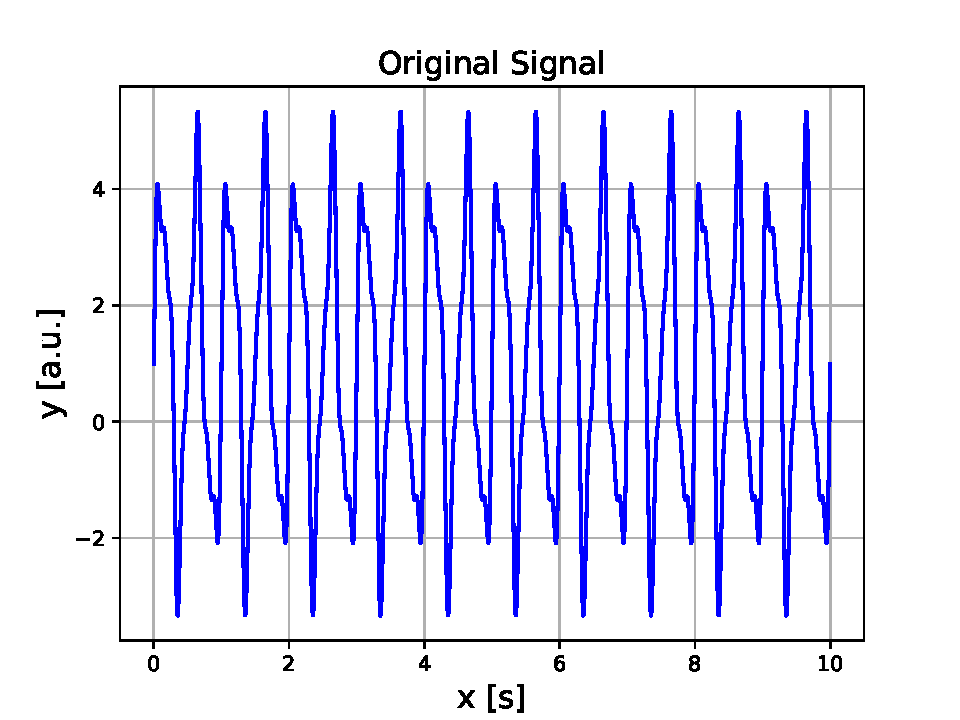
\includegraphics[scale=0.5]{img/signal_fft.pdf}
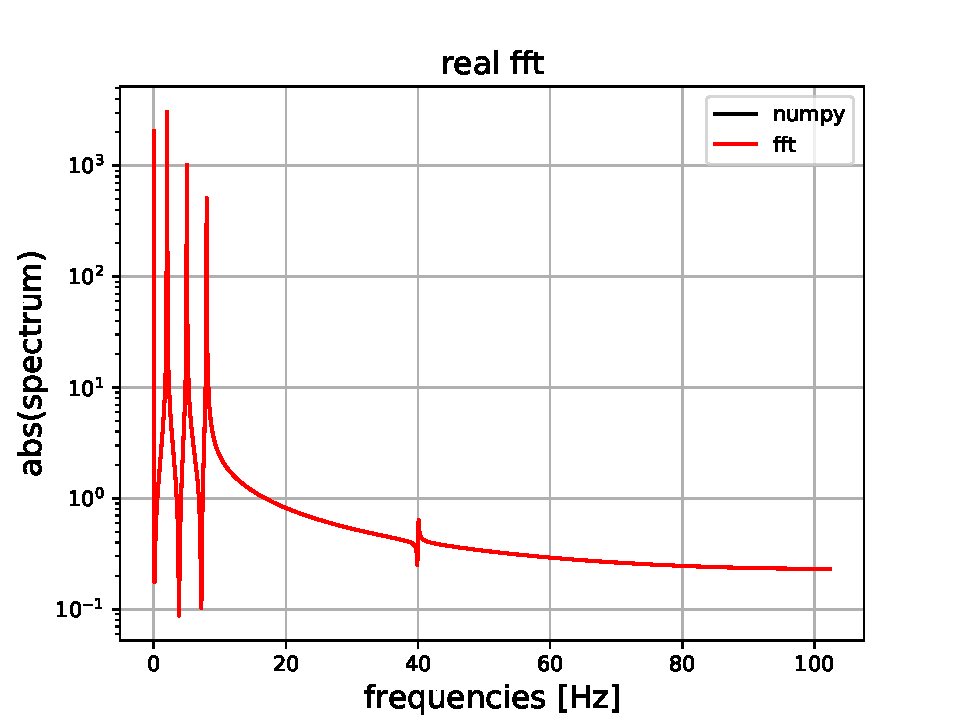
\includegraphics[scale=0.5]{img/sp_fft.pdf}
\end{figure}

\begin{center}
\makebox[\textwidth][c]{
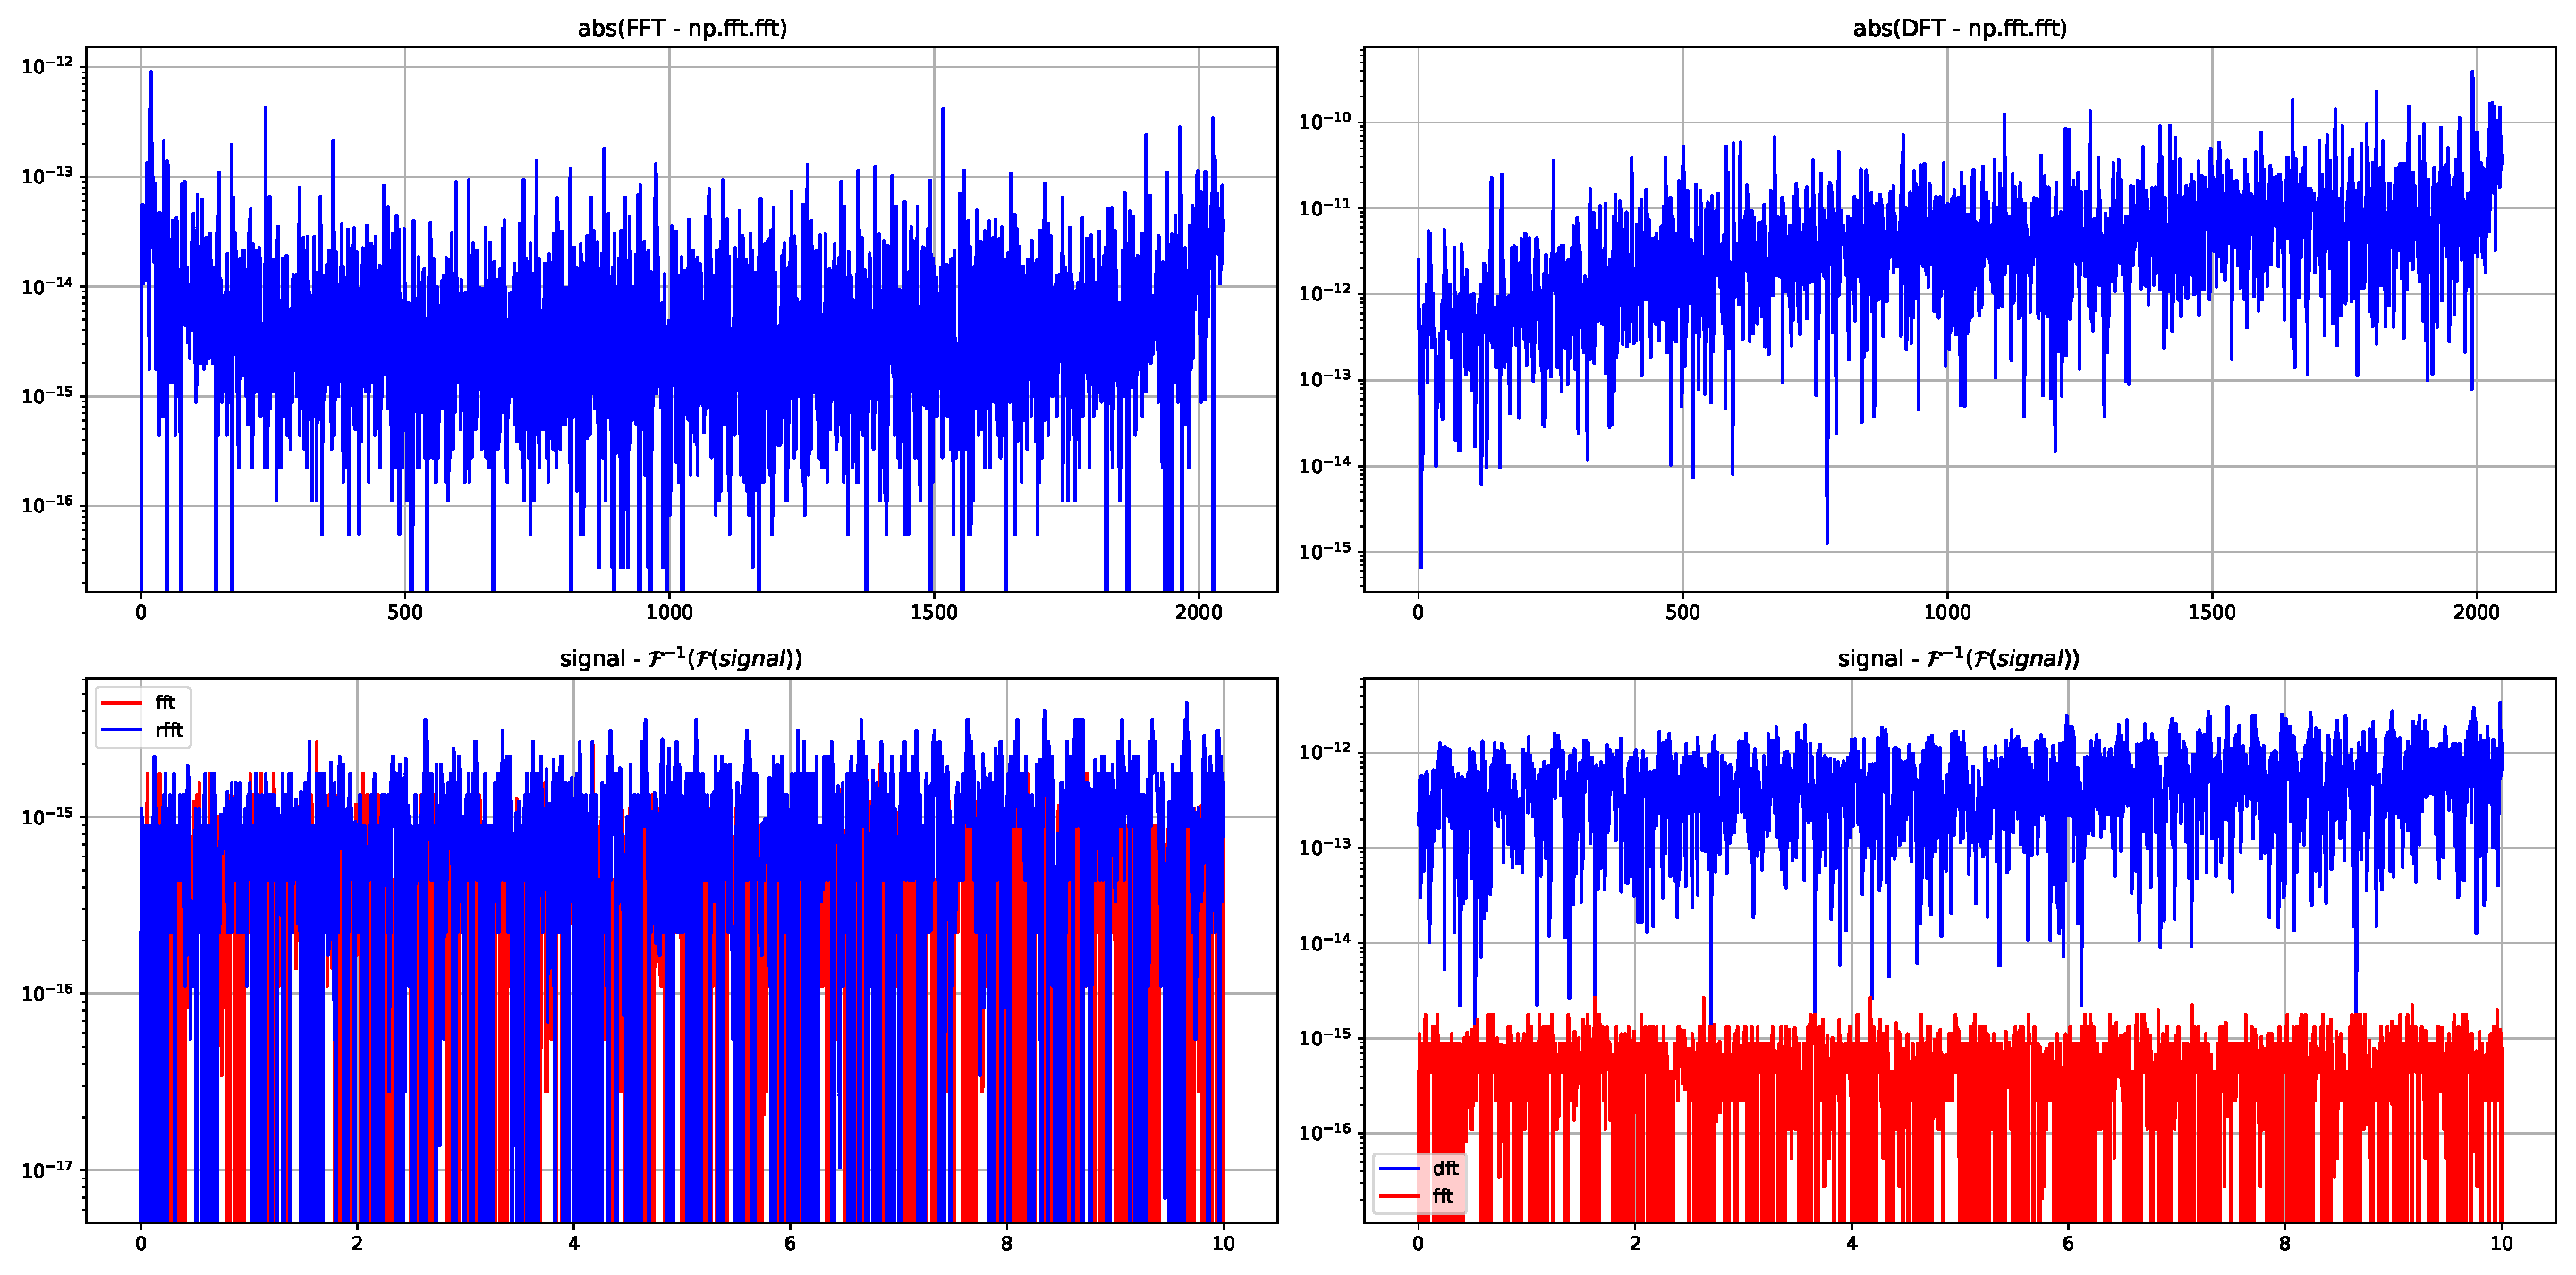
\includegraphics[scale=0.35]{img/cfr_fft.pdf}
}
\end{center}

\subsection{Applicazioni delle FFT}
\subsubsection{Derivate con FFT}
Vediamo ora una comoda applicazione delle fft, ovvero il calcolo delle derivate. In linea di principio quanto stiamo qui per fare si può fare con ogni tipo di polinomio con il quale possiamo sviluppare una certa funzione, ad esempio Legendre o Chebyshev; questo è chiamato metodo dei punti di collocazione. In serie di Fourier la cosa è piuttosto semplice, grazie alla sue proprietà matematiche, una derivata nello spazio (o nel tempo) corrisponde ad una moltiplicazione per $ik$ ($i\omega$) nello spazio degli impulsi (frequenze). Vediamo come:
\begin{lstlisting}[language=Python]
import numpy as np
import matplotlib.pyplot as plt

xi = 10         # estemo sinisto
xf = -xi        # estemo destro
N  = 1000       # numero punti
dx = (xf-xi)/N  # spaziatura punti

k = 2*np.pi*np.fft.fftfreq(N, dx) # vettore d'onda

#============================== CASO TRANQUILLO ==============================
x = np.linspace(xi, xf, N)                  # array posizioni
f = np.sin(x)*np.exp(-x**2/10)              # funzione di cui calcolare la derivata
g = np.cos(x)*np.exp(-x**2/10) - 2/10*x*f   # derivata analitica

f_hat  = np.fft.fft(f)       # trasformo con fourier
df_hat = 1j*k*f_hat          # moltiplico per l'impulso
df     = np.fft.ifft(df_hat) # derivata nello spazio

plt.figure(1)

plt.subplot(321)
plt.title('funzione', fontsize=15)
plt.ylabel('f', fontsize=15)
plt.plot(x, f)
plt.grid()

plt.subplot(323)
plt.title('Confronto derivate ', fontsize=15)
plt.ylabel('derivata', fontsize=15)
plt.plot(x, g)
plt.plot(x, df)
plt.grid()

plt.subplot(325)
plt.title('differenza fra derivata analitica e numerica', fontsize=15)
plt.ylabel('erorre globale derivata', fontsize=15)
plt.xlabel("X", fontsize=15)
plt.plot(x, abs(g-df))
plt.yscale('log')
plt.grid()
#============================== CASO MENO TRANQUILLO ==============================

def f():
    '''funzione
    '''
    y = []
    for xi in x:
        if xi < -5 :
            y.append(0)
        if xi > -5 and xi < 0:
            y.append(xi + 5)
        if xi > 0 and xi < 5:
            y.append(-xi + 5)
        if xi > 5:
            y.append(0)
    return np.array(y)

def g():
    ''' derivata analitica
    '''
    y = []
    for xi in x:
        if xi < -5 :
            y.append(0)
        if xi > -5 and xi < 0:
            y.append(1)
        if xi > 0 and xi < 5:
            y.append(-1)
        if xi > 5:
            y.append(0)
    return np.array(y)

f = f()
g = g()

f_hat  = np.fft.fft(f)       # trasformo con fourier
df_hat = 1j*k*f_hat          # moltiplico per l'impulso
df     = np.fft.ifft(df_hat) # derivata nello spazio

plt.subplot(322)
plt.title('funzione', fontsize=15)
plt.ylabel('f', fontsize=15)
plt.plot(x, f)
plt.grid()

plt.subplot(324)
plt.title('Confronto derivate ', fontsize=15)
plt.ylabel('derivata', fontsize=15)
plt.plot(x, g)
plt.plot(x, df)
plt.grid()

plt.subplot(326)
plt.title('differenza fra derivata analitica e numerica', fontsize=15)
plt.ylabel('erorre globale derivata', fontsize=15)
plt.xlabel("X", fontsize=15)
plt.plot(x, abs(g-df))
plt.yscale('log')
plt.grid()

plt.show()
\end{lstlisting}


\begin{center}
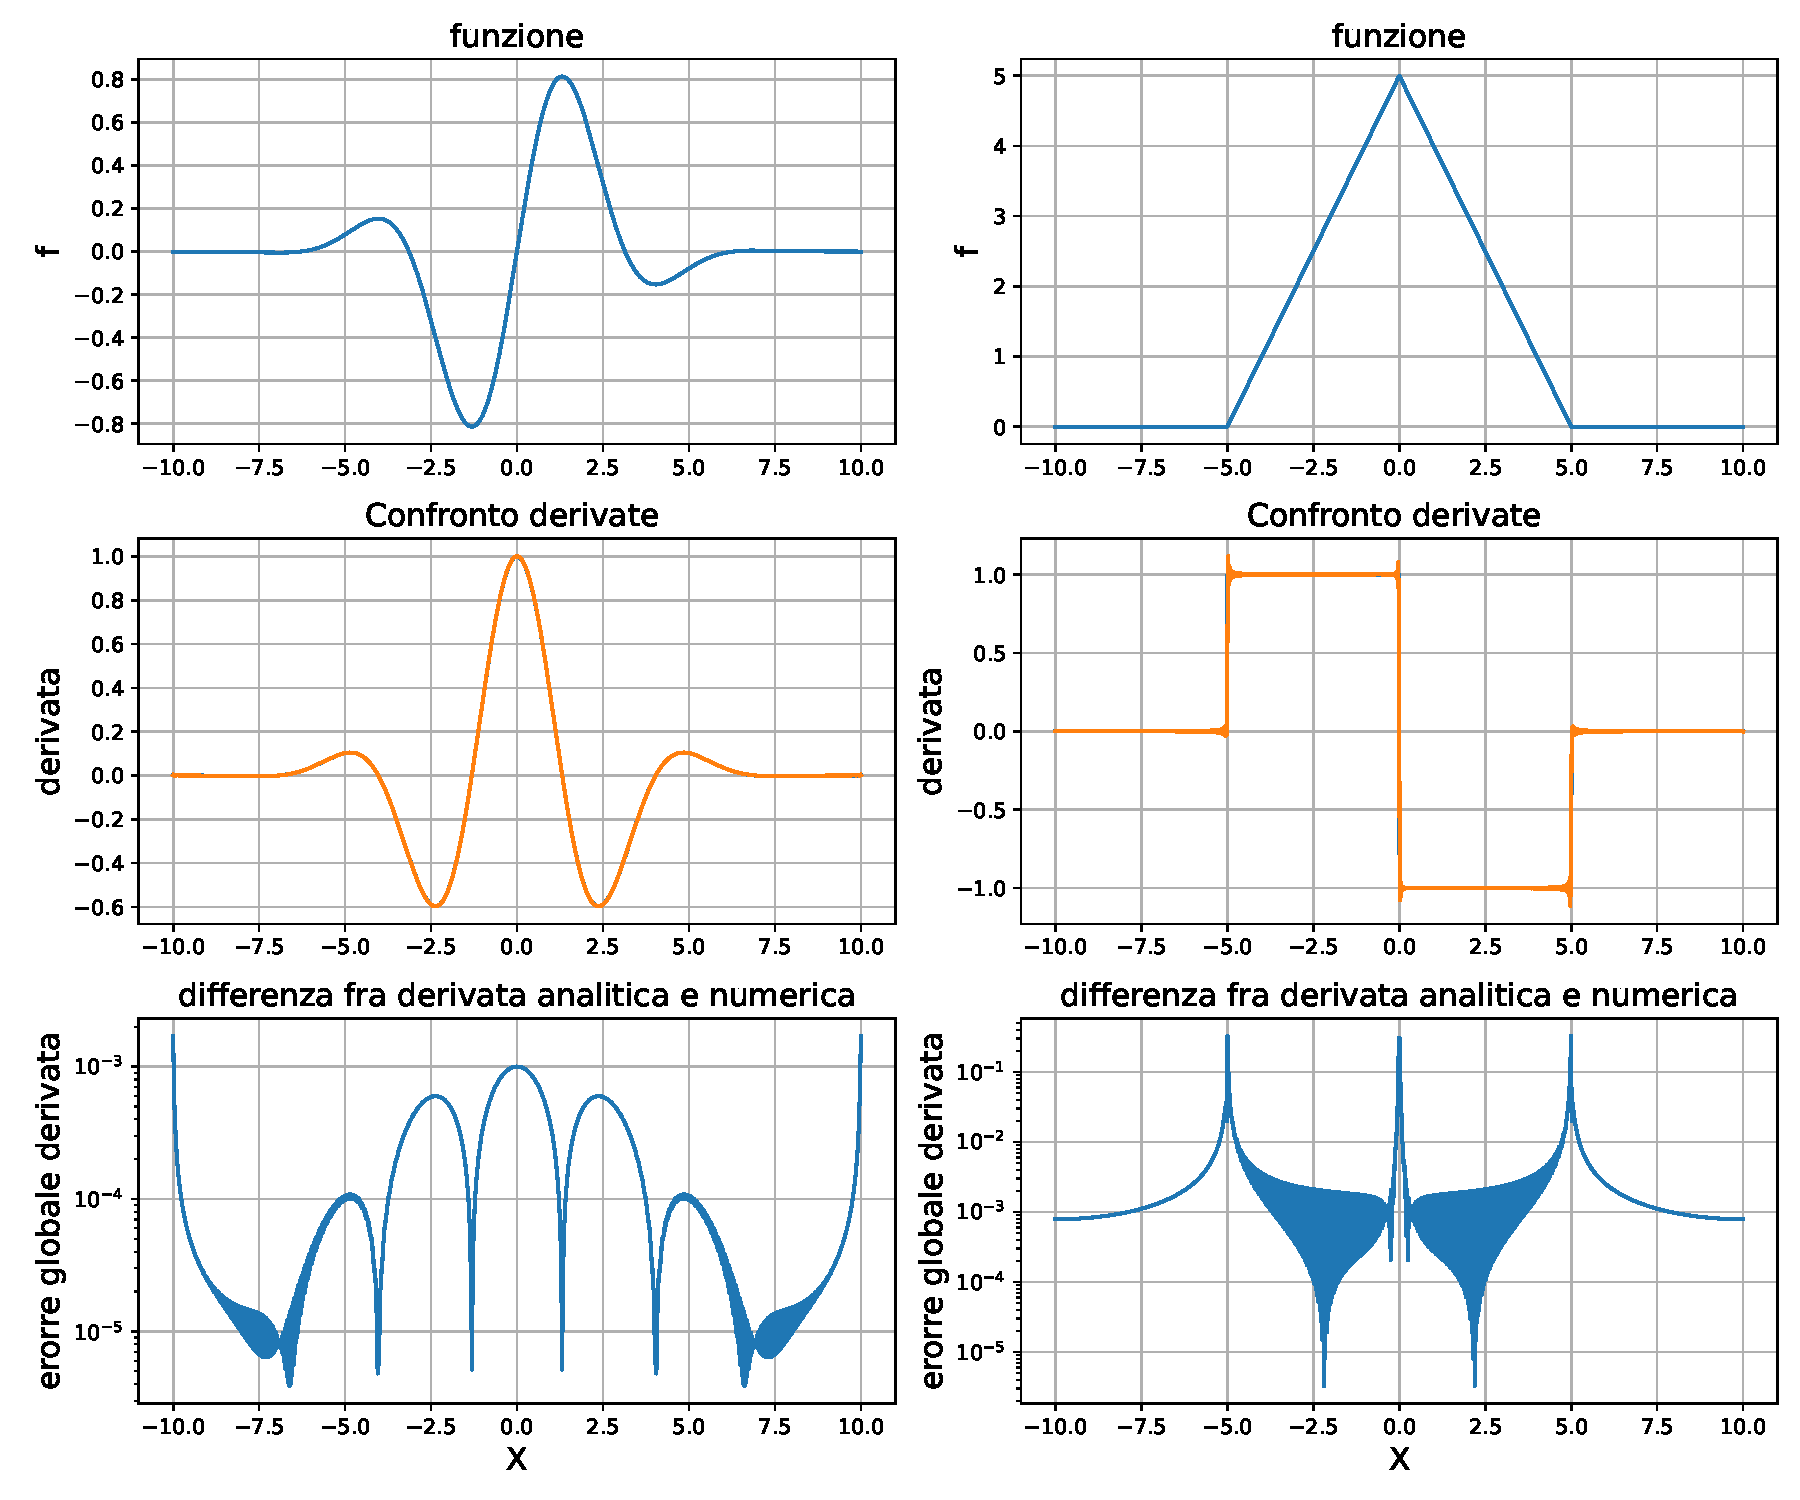
\includegraphics[scale=0.5]{img/cfr_derive_fft.pdf}
\end{center}

Si vede facilmente come nel caso della funzione a tratti la questione sia più delicata, già ad occhio vediamo dei piccoli spike ai bordi dove la funzione cambia e la derivata ha un gradino, inoltre l'errore è maggiore. 
\subsubsection{Equazione di Burgers}
Fare le derivate con le fft inoltre ci dà un'interessante prospettiva sulle PDE, infatti passando in trasformata, una PDE diventa una più tranquilla ODE, vediamo un semplice esempio. consideriamo l'equazione:
\begin{equation}
\frac{\partial u(t, x)}{\partial t} + u(t, x) \frac{\partial u(t, x)}{\partial x} = \nu \frac{\partial^2 u(t, x)}{\partial x^2} \quad,
\end{equation}
nota come equazione di Burgers, un'equazione abbastanza usale in fluidodinamica che ad esempio modelizza la formazione di un fronte d'onda ad esempio gli shock. Non so se nei corsi di fluidodinamica si veda, vi basti sapere che, come quasi tutto, si parte da:
\begin{equation}
\begin{cases}
\partial_t \rho + \partial_x (\rho v) = 0 \\
\partial_t (\rho v) + \partial_x (\rho v^2 + P) = \nu \partial_x^2 v
\end{cases}
\end{equation}
Assumendo come equazione di stato una politropica ed espandendo la densità e la velocità in serie di perturbazioni [e.g. $v = v_0 + v_1 + ...$, $\rho = \rho_0 + \rho_1 + ...$, (in genere $v_0$=0)] si ottiene che $\rho_1$ soddisfa l'equazione di Burgers.
 \'E facile vedere che passando in trasformata di nello spazio la nostra equazione diventa un'ode nel tempo:
\begin{equation}
\frac{\partial u(t, k)}{\partial t} + u(t, k) (i k u(t, k)) = \nu (- k^2 u(t, k)) \quad.
\end{equation}
Qui usiamo "scipy.integrate.odeint" per risolvere l'equazione, in una delle appendici, anzi due a vol essere precisi, sono trattati degli algoritmi risolutivi. 
Vediamo le poche righe di codice necessarie:

\begin{lstlisting}[language=Python]
"""
code to solve burger equation using fourier trasform in space
"""
import numpy as np
import matplotlib.pyplot as plt
from scipy.integrate import odeint
import matplotlib.animation as animation

#=============================================================
# Parameters
#=============================================================

L = 1
T = 0.31

dx = 0.001
dt = 0.001
nu = 0.005

Nx = int(L/dx)
Nt = int(T/dt)

t = np.linspace(0, T, Nt)
x = np.linspace(0, L, Nx)

# wave number
k = 2*np.pi*np.fft.fftfreq(Nx, dx)
# Initial conditions
u0 = np.sin(2*np.pi*x)

#=============================================================
# Solutions
#=============================================================

def eq(u, t, k, nu):
    '''
    equation to be solved in spatial transform
    '''
    u_hat = np.fft.fft(u)
    du_hat = 1j*k*u_hat    # first  derivative
    ddu_hat = -k**2*u_hat  # second derivative

    #antitrasform
    du = np.fft.ifft(du_hat)
    ddu = np.fft.ifft(ddu_hat)

    #pde in time and space -> ode in time
    u_t = -u*du + nu*ddu

    return u_t.real


sol = odeint(eq, u0, t, args=(k, nu,)).T


#=============================================================
# Animations
#=============================================================

fig = plt.figure(2)
plt.xlim(np.min(x), np.max(x))
plt.ylim(np.min(sol), np.max(sol))

line, = plt.plot([], [], 'b')
def animate(i):
    line.set_data(x, sol[:,i])
    return line,

anim = animation.FuncAnimation(fig, animate, frames=Nt, interval=5, blit=True, repeat=True)

plt.grid()
plt.title('burger equation')
plt.xlabel('Distanza')
plt.ylabel('ampiezza')

#anim.save('buger.mp4', fps=30, extra_args=['-vcodec', 'libx264'])

plt.show()
\end{lstlisting}
Eseguendo il codice vedrete l'animazione del fronte d'onda crearsi e grazie al termine diffusivo se ne evita la rottura. 
\subsubsection{Equazione di Schrödinger}
La scorsa lezione abbiamo visto come risolvere l'equazione di Schrödinger nel caso stazionario, ora vogliamo aggiungere il tempo e quindi vedere come una funzione d'onda evolve. L'equazione adesso diventa:
\begin{equation}
i \frac{\partial \psi}{\partial t} = H \psi .
\end{equation}
Assumiamo intanto che l'hamiltoniana non dipenda dal tempo (cfr. si conserva l'energia). Notiamo subito una cosa: chiaramente questa equazione è una PDE e modulo un'unità immaginaria è praticamente un'equazione diffusiva, tipo quella del calore. Si potrebbe quindi pensare di procedere allo stesso modo (proprio per l'equazione del calore è riportato un esempio in una delle appendici); c'è però un caveat: dato il suo significato di densità di probabilità è necessario che la psi sia normalizzata o per meglio dire e che la norma sia conservata durante l'evoluzione quindi il nostro algoritmo deve essere unitario. Sappiamo però per l'assunzione fatta precedentemente che la soluzione è:
\begin{equation}
\psi(t, x) = e^{-iHt} \psi(0, x) .
\end{equation}
Tutto molto tranquillo e tutto molto unitario, no? No chiaramente, $H$ è una matrice, e il suo esponenziale (in paroloni mi pare si dicesse implementazione unitaria) è definito con la serie di potenze, che non vogliamo star qui a calcolare. Idea: sviluppiamo per piccoli tempi $e^{-iH \delta t} \simeq 1 - i H \delta t$ e applichiamo tutto ciò alla condizione iniziale $\psi(0, x)$. Sorge un nuovo problema: abbiamo perso l'unitarietà, il modulo quadro non si conserva. Quello che si può fare per risolvere è noto come split operator:
\begin{equation}
e^{iH \delta t/2} \psi(t+\delta t, x) = e^{-iH \delta t/2} \psi(t, x) ,
\end{equation}
ovvero la funzione d'onda al tempo $t+\delta t$ evoluta indietro di $\delta t /2$ è uguale alla funzione d'onda al tempo $t$ evoluta in avanti di $\delta t/2$. Quindi approssimando sempre l'esponenziale al prim'ordine si ha:
\begin{equation}
\psi(t+\delta t, x) = \frac{1-iH \delta t/2}{1 + iH \delta t/2} \psi(t, x) .
\end{equation}
Mi perdonerete l'abuso di notazione, ovviamente dividere per $1+iH \delta t/2$ vuol dire invertire la matrice, ovvero risolvere un sistema; scriviamo così solo per renderci conto del fatto che quel coefficiente è della forma: numero complesso diviso il suo coniugato, e per cui ha modulo uno, garantendo l'unitarietà dell'evoluzione. Si ok molto bello ma la trasformata di Fourier?
Questo metodo può essere migliorato proprio grazie ad essa. Presa $H=T+V$, vale:
\begin{equation}
e^{-iH \delta t} = e^{-iV \delta t/2}e^{-iP \delta t}e^{-i V \delta t/2} + \mathcal{O}(\delta t^3).
\end{equation}
Una cosa simile verrà usata nella prossima lezione quando parleremo brevemente degli integratori simplettici. Perché facciamo questa divisone? Questi tre termini sono più facili da calcolare? Noi vogliamo calcolare l'operatore di evoluzione temporale ma senza dover esponenziare una matrice (In termini di matrici $T$ e $V$ hanno la forma vista nella lezione precedente). Facendo cosi vediamo subito i termini dipendenti da V si calcolano veloci in quanto se la matrice è diagonale l'espansione in serie mi da gli esponenziali delle entrare. Quindi vorremo poter diagonalizzare anche T, quindi l'impulso. Ma per andare dalla base della posizione a quella dei momenti si esegue proprio una trasformata di Fourier. Quindi in quella base $T$ sarà una matrice diagonale contenente i valori (al quadrato) che l'impulso può assumere (sempre nella nostra scatola di lato L in quanto abbiamo discretizzato, come sopra, lo spazio). La regola iterativa è dunque:
\begin{equation}
\psi(t+\delta t, x) = e^{-iV \delta t/2}\text{FFT}^{-1}(e^{-iP \delta t}\text{FFT}(e^{-i V \delta t/2}\psi(t, x))).
\end{equation}
Vediamo ora quindi il codice:
\begin{lstlisting}[language=Python]
"""
Code for the solution of Schrodinger's time dependent equation
via split operator method but unlike tunnel_barrier.py using a FFT.
Now the idea is tu use:
exp(1j (T+V) dt) = exp(1j V dt/2) exp(1j T dt) exp(1j V dt/2) + O(dt^3)
and to compute exp(1j T dt) we go in momentum space where T is diagonal
so it easy to compute, so we must use FFT to go from x space to p space
"""
import numpy as np
import matplotlib.pyplot as plt
import matplotlib.animation as animation

#=========================================================
# Initial wave function ad potential
#=========================================================

def U(x):
    ''' harmonic potential
    '''
    return 0.5*x**2

def psi_inc(x, x0, a, k):
    ''' Initial wave function
    '''

    A = 1. / np.sqrt( 2 * np.pi * a**2 ) # normalizzation
    K1 = np.exp( - ( x - x0 )**2 / ( 2. * a**2 ) )
    K2 = np.exp( 1j * k * x )
    # let's multiply by five so the animation is prettier
    return A * K1 * K2 * 5

#=========================================================
# Computational parameters
#=========================================================

n  = 1000                    # Number of points
xr = 10                      # Right boundary
xl = -xr                     # Left boundary
L  = xr - xl                 # Size of box
x  = np.linspace(xl, xr, n)  # Grid on x axis
dx = np.diff(x)[0]           # Step size
dt = 1e-3                    # Time step
T  = 10                      # Total time of simulation
ts = int(T/dt)               # Number of step in time

# Initializzation of gaussian wave packet
psi = psi_inc(x, -1.2, 0.5, 0.3)
PSI = []
PSI.append(abs(psi)**2)

#=========================================================
# Build the propagator in x and k space
#=========================================================

# Every possible value of momentum
k   = 2*np.pi*np.fft.fftfreq(n, dx)
# Propagator 
U_r = np.exp(-1j * U(x) * dt/2)  # Half step in space
U_k = np.exp(-1j * k**2/2 * dt)  # Full step in momentum

# Time evolution
for _ in range(ts):
    psi = U_r * psi
    
    psi_k = np.fft.fft(psi)
    psi_k = U_k * psi_k
    
    psi = np.fft.ifft(psi_k)
    psi = U_r * psi
    
    PSI.append(abs(psi)**2)

#=========================================================
# Animation
#=========================================================

fig = plt.figure()
plt.title("Gaussian packet propagation")
plt.plot(x, U(x), label='$V(x)$', color='black')
plt.grid()

plt.ylim(-0.0, np.max(PSI))
plt.xlim(-5, 5)

line, = plt.plot([], [], 'b', label=r"$|\psi(x, t)|^2$")

def animate(i):
    line.set_data(x, PSI[i])
    return line,

plt.legend(loc='best')

anim = animation.FuncAnimation(fig, animate, frames=np.arange(0, ts, 10), 
                               interval=1, blit=True, repeat=True)

#anim.save('ho.mp4', fps=30, extra_args=['-vcodec', 'libx264'])

plt.show()
\end{lstlisting}
In questo caso abbiamo nuovamente usato un potenziale armonico e possiamo vedere l'oscillazione della funzione d'onda nel nostro potenziale. Adesso ho due domande per voi: se rendete il pacchetto gaussiano iniziale più stretto la simulazione non viene bene; perché? Provate inoltre a fare l'evoluzione nel tempo immaginario $it=\beta$ (capisco sia un tempo ma concedetemi di chiamarlo $\beta$); ora perdiamo l'unitarietà quindi ad ogni passo bisogna normalizzare la psi. Cosa succede al nostro sistema? come pensate che evolva?
\subsubsection{Altre applicazioni}
Anche se non le esponiamo è interessante dire come la fft sia molto utile anche nell'analisi dati. Ad esempio se voglia filtrare un segnale si tratterebbe di fare una convoluzione tra segnale di input e il vostro filtro, ma le convoluzioni nello spazio della trasformata sono semplici prodotti. O magari anche capire se vi è o meno una componente debole ad una data frequenza nel vostro segnale: prendete ad esempio il segnale con cui abbiamo fatto sopra i test; se gli aggiungete del rumore, la componente a 40 Hz nello spetto magari non si vede. Ma se il segnale è a media zero vedrete che vi è un picco in negativo molto importante a frequenza nulla nella trasformata; perciò vi basta moltiplicare tutto il segna per, un seno ad esempio, alla stessa frequenza della componente che cercate; ciò creerà un battimento e una delle due omega sarà nulla. Per cui nella FFT il profondo picco negati sarà notevolmente ridotto, e ciò vi fa quindi capire la presenza di quell'armonica. Non so quanto sono stato chiaro, magari più il là fornirò degli esempi di codice. Intanto magari potete provare a scriverli da voi.
\newpage

\section{Terza Lezione A}
\subsection{Programmazione a oggetti: problema N-body}
Python è un linguaggio che permette la programmazione ad oggetti. Molto di Python stesso è scritto con programmazione orientata ad oggetti. Lo scopo è quello di illustrare un semplice esempio di utilizzo creando una piccola simulazione ad N corpi. Per programmare ad ogetti si utilizza quelle che sono chiamate classi; fondamentalmente creare una classe vuol dire definire un oggetto. All'interno della classe è possibile definire delle funzioni che verranno chiamati metodi. Alcuni metodi sono particolari e sono contrassegnati da doppi underscore, e.g: "\_\_init\_\_, \_\_iter\_\_, \_\_next\_\_, \_\_call\_\_"; qui ci limiteremo al primo, in quanto necessario, e l'ultimo poiché può essere utile. I due nel mezzo permettono di costruire un "iterabile", parola che non dovrebbe esservi nuova; così come l'ultimo permette di costruire un oggetto "chiamabile" ("callable" anche questo non dovrebbe sembrarvi nuovo). Cominciamo quindi, nell'ottica della nostra simulazione a N corpi, a definire la nostra classe che ci permetterà di costruire i protagonisti della nostra simulazione (ci limiteremo per semplicità a vincolare la dinamica su un piano):
\begin{lstlisting}[language=Python]
import numpy as np
import random as rn
import matplotlib.pyplot as plt
from matplotlib import animation

class Body:
    """
    Classe che rappresenta una pallina
    intesa come ogetto puntiforme
    """

    def __init__(self, x, y, vx, vy, m=1):
        """
        costruttore della classe, verra' chiamato
        quando creeremo l'istanza della classe, (i.e. b=Body()
        b e' chiamata istanza).
        In input prende la posizione, la velocita' e massa
        che sono le quantita' che identificano il corpo
        che saranno gli attributi della classe;
        il costruttore e' un particolare metodi della
        classe per questo si utilizzano gli underscore.
        il primo parametro che passiamo (self) rappresenta
        l'istanza della classe (self e' un nome di default)
        questo perche' la classe e' un modello generico che
        deve valere per ogni corpo.
        """
        #posizione
        self.x = x
        self.y = y
        #velocita'
        self.vx = vx
        self.vy = vy
        #massa
        self.m = m
    
    #aggiornamento posizione e velocita' con eulero
    def n_vel(self, fx, fy, dt):
        """
        ad ogni metodo della classe viene passato
        come primo argomento self , quindi l ' istanza
        date le componenti della forza e il passo temporale
        aggiorno le componenti della velocita'
        """
        self.vx += fx*dt
        self.vy += fy*dt

    def n_pos(self, dt):
        """
        dato il passo temporale aggiorno le posizioni
        """
        self.x += self.vx*dt
        self.y += self.vy*dt

\end{lstlisting}
Non è propriamente necessario usare i metodi per cambiare gli attributi di una classe, si possono utilizzare cose quali le property e i setter, ma non ce ne cureremo. Dunque ora abbiamo qualcosa che ci permette di creare i nostri oggetti, ognuno con caratteristiche (valori degli attributi) diversi. Abbiamo poi due metodi che ci permetto di aggiornare le quantità fisiche e dare una dinamica a tutti i nostri corpi. Vediamo ora, sempre grazie ad un altra classe come implementare la nostra simulazione. Useremo per evitare divergenze in caso di incontri ravvicinati (del terzo tipo) quella che è la tecnica del softening, cioè il potenziale kepleriano sarà:
\begin{equation}
V(r) = - \frac{1}{\sqrt{r^2 + \epsilon}}
\end{equation}
con $\epsilon$ chiamato appunto parametro di softening. Così anche se i pianeti sono molto vicini La forza tra essi non diverge. Se vogliamo simulare una normale orbita possiamo sempre settare a zero questo parametro.
\begin{lstlisting}[language=Python]
class Sistema:
    '''
    Classe per evoluzione del sistema.
    Viene utilizzata la tecnica del softening  per impedire
    divergenze nella foza, sp e' il parametro di softening
    
    Parameters
    ----------
    corpi : list
        lista di ogetti della classe Body
    G : float
        Costante di gravitazione universale (=1)
    sp : float, optional, default 0
        parametro di softening
    '''

    def __init__(self, corpi, G, sp=0):
        self.corpi = corpi
        self.G = G
        self.sp = sp

    def evolvo(self, dt):
        '''
        chimata ad ogni passo temporale, fa evolvere il sistema
        solo di uno step dt, la forza e' calcolata secondo la
        legge di gravitazione universale;
        '''

        for corpo_1 in self.corpi:

            fx = 0.0
            fy = 0.0

            for corpo_2 in self.corpi:
                if corpo_1 != corpo_2:

                    dx = corpo_2.x - corpo_1.x
                    dy = corpo_2.y - corpo_1.y

                    d = np.sqrt(dx**2 + dy**2 + self.sp)

                    fx += self.G * corpo_2.m * dx / d**3
                    fy += self.G * corpo_2.m * dy / d**3

            corpo_1.n_vel(fx, fy, dt)

        for corpo in self.corpi:
            corpo.n_pos(dt)

\end{lstlisting}
Fondamentalmente La nostra classe ci permette quindi di integrare le varie equazioni del moto. Importante notare il metodo con cui esse sono integrate: aggiorniamo prima tutte le velocità e poi tutte le posizioni. Questo è chiamato metodo di eulero simplettico. Ora mostriamo la parte conclusiva del codice per avviare la nostra simulazione:
\begin{lstlisting}[language=Python]
#===========================================================================
# Creating bodies and the system and computational parameters
#===========================================================================

rn.seed(69420)
dt = 1/20000
T  = int(2/dt)
E  = np.zeros(T)
L  = np.zeros(T)
G  = 1

# Number of body, must be even
N = 10
C = []
for n in range(N//2):
    '''
    two bodies are created at a time
    with equal and opposite velocity
    to keep the total momentum of the system zero
    '''
    v_x = rn.uniform(-0.5, 0.5)
    v_y = rn.uniform(-0.5, 0.5)
    C.append(Body(rn.uniform(-0.5, 0.5), rn.uniform(-0.5, 0.5), v_x, v_y))
    C.append(Body(rn.uniform(-0.5, 0.5), rn.uniform(-0.5, 0.5), -v_x, -v_y))
    

X = np.zeros((2, T, N)) # 2 because the motion is on a plane

# Creation of the system
soft = 0.01
sist = System( C, G, soft)

#===========================================================================
# Evolution
#===========================================================================

start = time.time()

for t in range(T):
    sist.update(dt)
    for n, body in enumerate(sist.bodies):
        X[:, t, n] = body.x, body.y

print("--- %s seconds ---" % (time.time() - start))

#===========================================================================
# Plot and animation
#===========================================================================

fig = plt.figure(0)
plt.grid()
plt.xlim(np.min(X[::2, :])-0.5, np.max(X[::2, :])+0.5)
plt.ylim(np.min(X[1::2,:])-0.5, np.max(X[1::2,:])+0.5)
colors = ['b']*N#plt.cm.jet(np.linspace(0, 1, N))

dot  = np.array([]) # for the planet

for c in colors:
    dot  = np.append(dot,  plt.plot([], [], 'o', c=c))

def animate(i):
    
    for k in range(N):
        
        dot[k].set_data(X[0, i, k], X[1, i, k])
    
    return dot

anim = animation.FuncAnimation(fig, animate, frames=np.arange(0, T, 50), interval=1, blit=True, repeat=True)


plt.title('N body problem', fontsize=20)
plt.xlabel('X(t)', fontsize=20)
plt.ylabel('Y(t)', fontsize=20)

# Ucomment to save the animation, extra_args for .mp4
#anim.save('N_body.gif', fps=50)# extra_args=['-vcodec', 'libx264']) 

plt.show()
\end{lstlisting}

Oltre ad n palline a caso, creiamo anche un sistema, un pianeta che orbita intorno a due stelle:
\begin{lstlisting}[language=Python]
# creation of body
C1 = Body(0.5,  0, 0, 20,  int(1e3))
C2 = Body(-0.5, 0, 0, -20, int(1e3))
C3 = Body(-1.5, 0, 0, 40,  int(1e1))
C  = [C1, C2, C3]
N  = len(C)
\end{lstlisting}
Ora in linea di principio la simulazione finisce qui. Tuttavia risulta interessante calcolare l'energia e il momento angolare del nostro sistema e vedere se esse, come ci si aspetteremmo, sono effettivamente conservate durante l'evoluzione del sistema. Mostreremo i risultati ma senza mostrare il codice che comunque trovate disponibile. Tra l'altro questa analisi la vogliamo fare mostrando soltanto il caso di tre corpi che si orbitano attorno in quanto nei due casi che mostreremo (due integratori diversi) le differenze sono apprezzabili. Usando N corpi creati a caso la conservazione dell'energia non si manifesta mai, a differenza, e vedremo perché, della conservazione del momento angolare. Per quanto riguarda la conservazione dell'energia probabilmente ciò è dovuto al fatto che, quelle scelte, non sono delle buone condizioni iniziali: in genere l'inizializzazione è affrontata in maniera più delicata (a noi interessava solo vedere l'animazione carina).
Da qui e dal tipo di integratore usato, che abbiamo citato prima nasce tutta un'interessante discussione sulla meccanica classica, che brevemente vogliamo trattare.
\subsection{Breve compendio di meccanica Hamiltoniana}
Allora come prima cosa diamo un paio di definizioni, cercando comunque di non essere troppo matematici (non dimostriamo nulla qui, lasciamo tutto all'eventuale curiosità dell'eventuale lettore):\\
Consideriamo inizialmente una 2-forma $\omega$ differenziale su una varietà liscia $M$. La 2-forma $\omega$ è chiamata simplettica se è chiusa e non degenere. Chiusa significa che la sua derivata esterna è nulla d$\omega = 0$; non vogliamo perdere tempo a spiegare cosa sia la derivata esterna, ma la potete vedere come una derivata che sia antisimmetica (cfr. tensore elettromagnetico: dato $A$ potenziale vettore d$A$ = $\partial_i A_j - \partial_j A_i = F_{ij}$). Non degenere significa invece che, per ogni punto $p \in M$, considerando lo spazio tangente al punto $T_pM$ (che è uno spazio vettoriale), si ha che per ogni vettore $x$ non nullo su questo spazio esiste un vettore $y$ tale che: $\omega(x, y) = 0$ solo per $y=0$. Dunque la coppia $(M, \omega)$ è una varietà simplettica.\\
Consideriamo ora una funzione liscia $H: M \to \mathbb{R}$ su una varietà simplettica $(M, \omega)$. Abbiamo allora che il campo vettoriale $X_H$ definito da $\omega(X_H, Y) = $ d$H(Y)$ è chiamato campo vettoriale hamiltoniano generato da $H$. La terna $(M, \omega, H)$ definisce un sistema hamiltoniano.\\
Inoltre è importante menzionare il seguente teorema: Sia $(M, \omega, H)$ un sistema hamiltoniano e sia $\Phi: \mathbb{R} \times M \to M$ il flusso generato dal campo vettoriale $X_H$. Allora $\forall t \in \mathbb{R}$  $\Phi_t$ è simplettico. Questo significa che il flusso non solo preserva la struttura simplettica, in particolare esso preserva la forma volume, il che vuol dire che preserva il volume dello spazio delle fasi. Inoltre il flusso esatto della nostra hamiltoniana è reversibile $\Phi_t^{-1} = \Phi_{-t}$ \\
Detto ciò vediamo di concretizzare un po'; supponiamo di avere una hamiltoniana della forma:
\begin{equation}
H(p, q) = T(p) + V(q) \quad.
\end{equation}
Se definiamo $x = (p, q)$ l'insieme di tutte le nostre variabili allora sappiamo che l'equazione del moto sono date dalla parentesi di poisson:
\begin{equation}
\dot{x} = X_H = \{x, H(x) \} \quad,
\end{equation}
la cui soluzione è:
\begin{equation}
x(\tau) = e^{\tau X_H} x(0) \quad.
\end{equation}
Abbiamo detto che vogliamo dunque integrare le nostre equazioni del moto. Assumiamo che dato un certo $n$ esistano certi coefficienti $c_1, \dots, c_k$ e $d_1, \dots, d_k$ tale che:
\begin{equation}\label{int}
e^{\tau X_H} = e^{\tau(X_T + X_V)} = \prod_{i=1}^k e^{\tau c_i X_T}e^{\tau d_i X_V} + \mathcal{O}(\tau^{n+1}) \quad,
\end{equation}
dove i $c_i$ e $d_i$ devono rispettare certi vincoli a seconda del valore di $n$, e a seconda del quale inoltre si ottengono diversi algoritmi: per $n=1$ abbiamo eluero simplettico (quello implementato sopra) mentre per $n=2$ abbiamo il leapfrog. Non ci metremo ora a calcolare questi coefficienti. Inoltre si dimostra, ma noi non lo facciamo, che trovare i $c_i$ e $d_i$ che soddisfano la (\ref{int}) è equivalente a trovare dei coefficienti $c_i$ e $d_i$ tali che:
\begin{equation}
\Phi_{\tau} = \prod_{i=1}^k e^{\tau c_i X_T}e^{\tau d_i X_V} = e^{\tau(X_T + X_V) + \mathcal{O}(\tau^{n+1})} \quad.
\end{equation}
\' E inoltre interessante notare che se consideriamo l'integratore di eulero: $\Phi_h = e^{h X_T}e^{h X_V}$ esso è soluzione esatta di un altro sistema hamiltoniano scritto come perturbazioni di $H$, che non è detto abbia le stessi simmetrie dell'hamiltoniana di partenza:
\begin{equation}
\overline{H} = H + hH_2 + h^2H_3 + \dots 
\end{equation}
dove gli $H_i$ si calcolano tramite parentesi di poisson espandendo in serie con la formula di Baker-Campbell-Hausdorff (BCH):
\begin{equation}
\begin{split}
\overline{X_H} &= \frac{1}{h} \ln(e^{h X_T}e^{h X_V}) \\
&= \underbrace{X_T + X_V}_{H} + h \underbrace{\frac{1}{2}[X_T, X_V]}_{H_2} + h^2 \underbrace{\frac{1}{12}([[X_T, X_V], X_V] + [[X_V, X_T], X_T])}_{H_3}  \quad .
\end{split}
\end{equation}
Più in generale per un integratore della forma: $\Phi_{h} = \prod_{i=1}^k e^{h c_i X_T}e^{h d_i X_V}$ esso è soluzione di:
\begin{equation}
\overline{H} = H + h^n H_{n+1} + \mathcal{O}(h^{n+1}) \quad,
\end{equation}
dove ora i vari $H_i$ saranno diversi ma il modo di calcolarli è sempre lo stesso.
Tornando a noi è stato implementato per fare un confronto anche un medoto simplettico del 4 ordine noto con il nome di Yoshida; scrivendo in coordinate lagrangiane la regola iterativa è:
\begin{align}
v_{i+1} &= v_{i} + d_{i} a(x_{i}) dt \\
x_{i+1} &= x_{i} + c_{i} v_{i+1} dt
\end{align}
dove i coefficienti valgono:
\begin{align}
 c_1 &= c_4 = \frac{1}{2(2-2^{1/3})} \hspace{10 mm} c_2 = c_3 = \frac{1-2^{1/3}}{2(2-2^{1/3})}, \\
 d_1 &= d_3 = \frac{1}{2-2^{1/3}}, \hspace{12.5 mm} d_2 = -\frac{2^{1/3}}{2-2^{1/3}}, \quad d_4 = 0.
\end{align}

Ultima cosa da far notare, ma molto interessante è che ogni integratore simplettico conserva il momento angolare, o più in generale è conservato qualsiasi generatore di trasformazioni puntuali lineari che sia una simmetria di $H$ (e.g. rotazioni, dilatazioni, traslazioni). Per trasformazioni del tipo:
\begin{align}
q_i & \to q_i + \epsilon A_i(q) = q_i + \epsilon(\Omega_{ij}q_j + n_i) , \\
p_i & \to p_i - \epsilon \Omega_{ij}p_j \quad,
\end{align}
dove $\Omega$ è una matrice $N \times N$ e $n$ è un vettore di coefficienti costanti. L'invarianza di $H$ si scrive come:
\begin{equation}
\frac{\partial H}{\partial q_i} \delta q_i + \frac{\partial H}{\partial p_i} \delta p_i = \epsilon \Bigg( \frac{\partial H}{\partial q_i} n_i + \frac{\partial H}{\partial q_i} \Omega_{ij}q_j - \frac{\partial H}{\partial p_i} \Omega_{ij}p_j \Bigg) = 0 \quad.
\end{equation}
Potete divertirvi a sostituire l'espressione data per le nuove coordinate date dall'integratore e far vedere che il generatore $G(p, q) = A_i p_i = \Omega_{ij} p_i q_j + n_i p_i$ è conservato.\\ Un modo magari più familiare per vedere tutto quel che abbiamo detto è quello dell'utilizzo delle trasformazioni canoniche.\\ Ricordiamo intanto che: $Q(q, p, t)$ e $P(q, p, t)$ sono trasformazioni canoniche se per una qualsiasi hamiltoniana  $H(q, p, t)$ si può trovare un'hamiltoniana $K(Q, P, t)$ tale per cui le equazioni del moto per $p$ e $q$ data da $H$, si trasformano in quelle date da $K$ in termini di $Q$ e $P$.\\
In termini di $x$, definito sopra, abbiamo che:
\begin{equation}
\dot{x} = \Gamma \frac{\partial H}{\partial x} \hspace{5 mm } \text{con} \hspace{5 mm} \Gamma = 
\begin{pmatrix}
0 & - \text{Id}_{N \times N} \\
\text{Id}_{N \times N} & 0 \\
\end{pmatrix}
\end{equation}
Facciamo ora una trasformazione $X(x)$ (si generalizza a anche a trasformazioni dipendenti dal tempo). Abbiamo quindi che:
\begin{equation}
\dot{X}_i = \frac{\partial X_i}{\partial x_j} \dot{x}_j = \frac{\partial X_i}{\partial x_j} \Gamma_{jl} \frac{\partial H}{\partial x_l} = \frac{\partial X_i}{\partial x_j} \Gamma_{jl} \frac{\partial H}{\partial X_k} \frac{\partial X_k}{\partial x_l}  =  J_{ij}\Gamma_{jl}J^T_{lk} \frac{\partial H}{\partial X_k} = (J \Gamma J^T)_{ik} \frac{\partial H}{\partial X_k}
\end{equation}
Per cui si arriva a:
\begin{equation}
J \Gamma J^T = \Gamma,
\end{equation}
equazione che, in termini di matrici, definisce il gruppo simplettico.
Diciamo questo perché tra simpletticità e canonicità c'è un legame stretto: $X(x, t)$ è canonica se la sua matrice jacobiana è simplettica a tutti i tempi a meno di una costante cioè: $J \Gamma J^T = \alpha \Gamma$. Inoltre se abbiamo che:
\begin{equation}
\{A, B\}_x = \{A, B\}_X,
\end{equation}
la nostra trasformazione è simplettica. Ma sappiamo anche che verificare le parentesi di Poisson ci dà la canonicità della trasformazione:
\begin{equation}
X_i = \{X_i, H\}_x = \{X_i, H\}_X = \Gamma_{ij} \frac{\partial H}{\partial X_j}
\end{equation}
Facciamo quindi un esempio semplice per far vedere come il metodo di Eulero non sia simplettico ma quello da noi implementato sopra lo sia. Per semplicità consentitemi di considerare (piuttosto che $N$ corpi) la seguente:
\begin{equation}
H = \frac{p^2}{2} - \frac{1}{q}.
\end{equation} 
Il metodo di Eulero prevede:
\begin{align}
p(t+ \delta t)&=p(t) - \delta t \frac{\partial H(q(t), p(t))}{\partial q}\\
q(t+ \delta t)&=q(t) + \delta t \frac{\partial H(q(t), p(t))}{\partial p}
\end{align}
Nel nostro caso abbiamo:
\begin{align}
p(t+ \delta t)&=p(t) - \delta t \frac{1}{q^2(t)}\\
q(t+ \delta t)&=q(t) + \delta t p(t)
\end{align}
Per verificare la canonicità va dunque calcolata la:
\begin{equation}
\begin{split}
\{q(t+ \delta t), p(t+ \delta t)\} &= \{q(t), p(t)\} - \delta t \{q(t), q^{-2}(t)\} + \delta t \{p(t), p(t)\} - \delta t^2 \{p(t), q^{-2}(t) \} \\
 &= 1 - \delta t^2 2 q^{-3}(t) .
\end{split} 
\end{equation}
Vediamo dunque che la trasformazione non è canonica a tutti gli ordini in $\delta t$. Il metodo di Eulero simplettico invece ci dice:
\begin{align}
p(t+ \delta t)&=p(t) - \delta t \frac{\partial H(q(t), p(t+ \delta t))}{\partial q}\\
q(t+ \delta t)&=q(t) + \delta t \frac{\partial H(q(t), p(t+ \delta t))}{\partial p}
\end{align}
Che nel nostro caso diventa:
\begin{align}
p(t+ \delta t) &=p(t) - \delta t \frac{1}{q^2(t)}\\
q(t+ \delta t) &=q(t) + \delta t p(t+ \delta t) = q(t) + \delta t p(t) - \delta t^2 \frac{1}{q^2(t)}
\end{align}
Per cui abbiamo:
\begin{equation}
\begin{split}
\{q(t+ \delta t), p(t+ \delta t)\} &= \{q(t), p(t)\} - \\
&- \delta t( \{q(t), q^{-2}(t)\} - \{p(t), p(t)\}) - \\
&- \delta t^2( \{p(t), q^{-2}(t) \} + \{q^{-2}(t), p(t) \} - \{ q^{-2}(t), q^{-2}(t)\}) \\
&=1
\end{split} 
\end{equation}
Si vede bene dunque che la trasformazione è canonica per ogni $\delta t$; dato che il termine che prima rompeva la canonicità ora si cancella con un altro termine, mentre gli altri sono tranquillamente nulli. Potete se volete verificare che Eulero simplettico è dato dalla seguente funzione generatrice:
\begin{equation}
F_2(q(t), p(t + \delta t) ) = q(t) p(t + \delta t) + \delta t H(q(t), p(t + \delta t)).
\end{equation}
Il problema di questo metodo è però che non è reversibile. Si può però combinare con la variante in cui si usa $q(t+\delta t)$ per aggiornare $p(t)$, dando così vita ad un metodo del secondo ordine che è il leapfrog citato prima. Il quale è reversibile.
Vediamo ora i risultati, dal punto di vista delle conservazioni, di due integratori (Eulero simplettico e Yoshida del quarto ordine):
\FloatBarrier
\begin{figure}
\centering
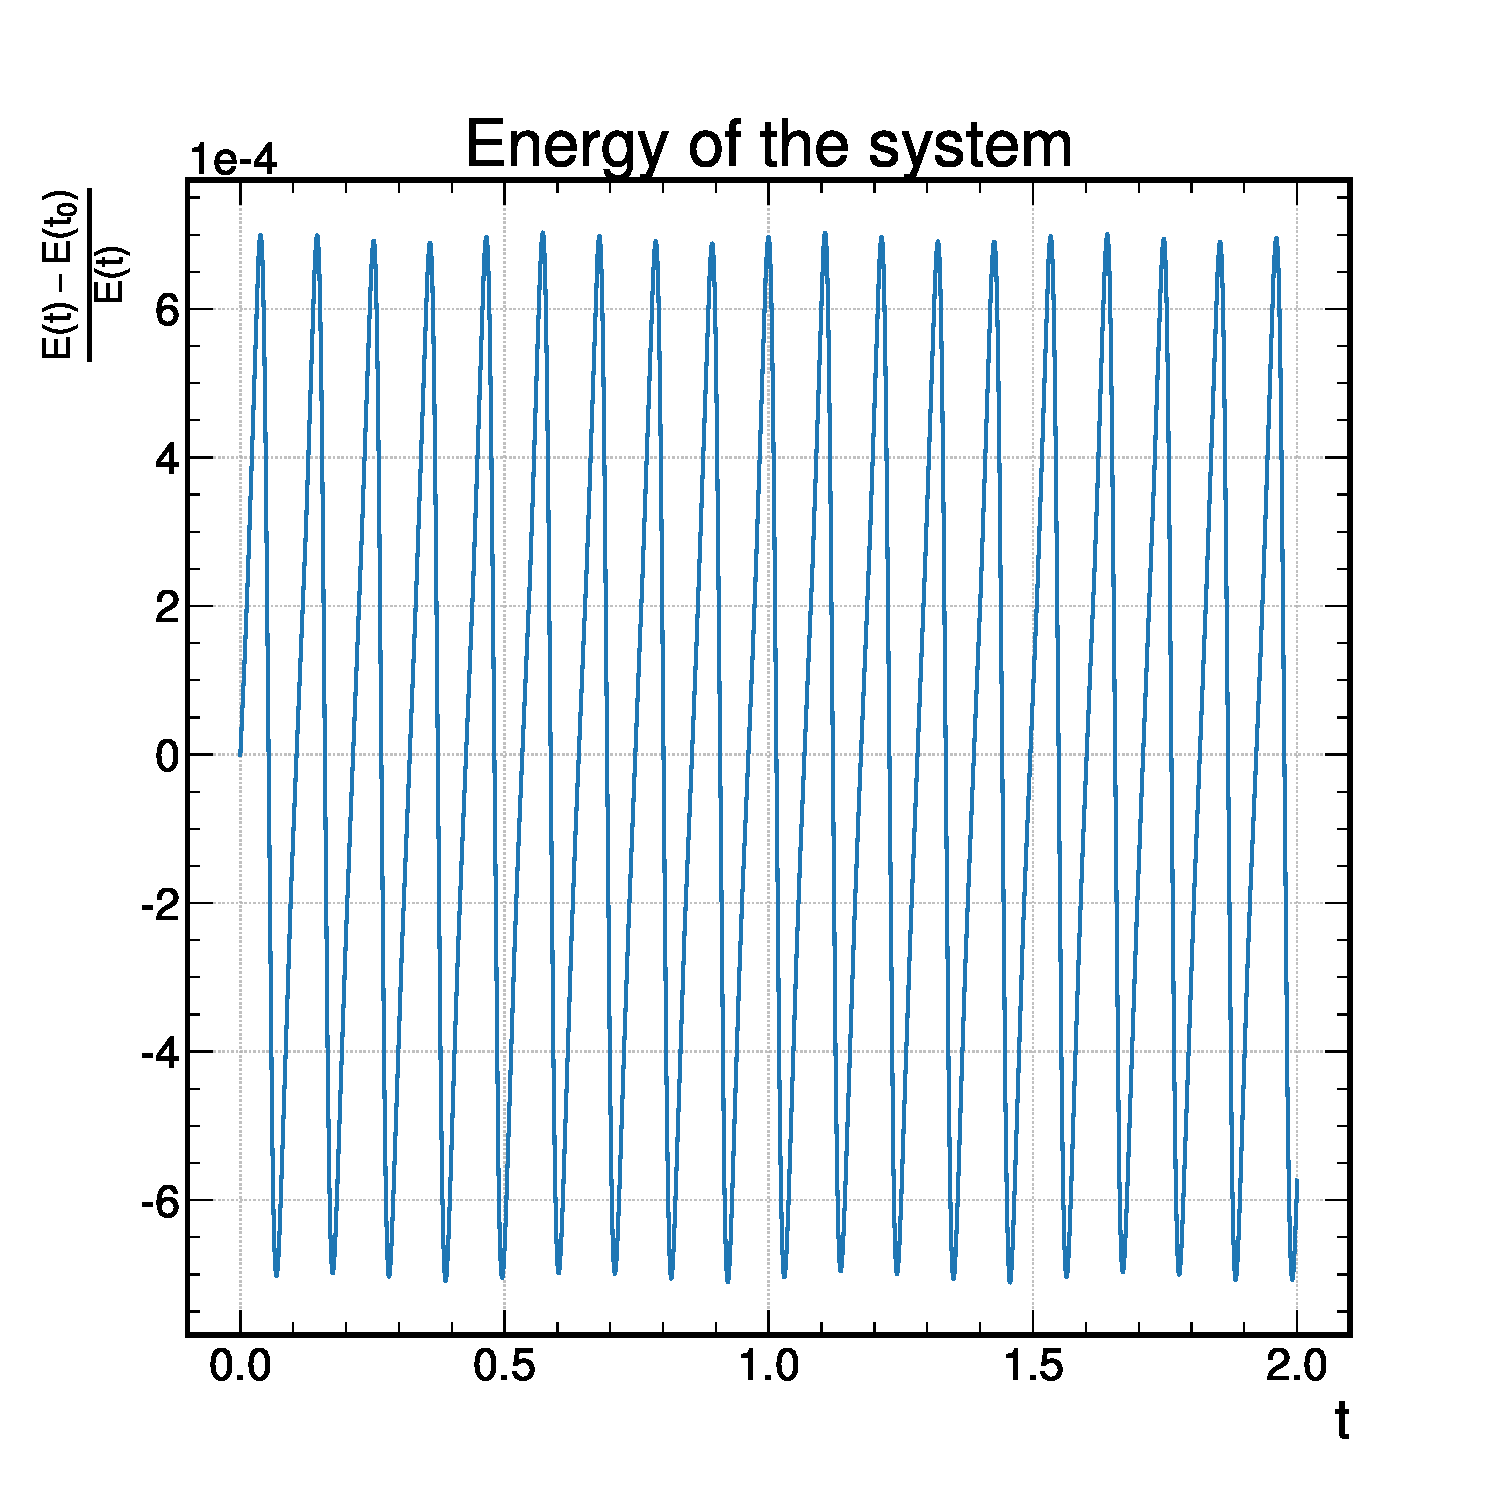
\includegraphics[scale=0.3]{img/ene_euler_simpl.pdf}
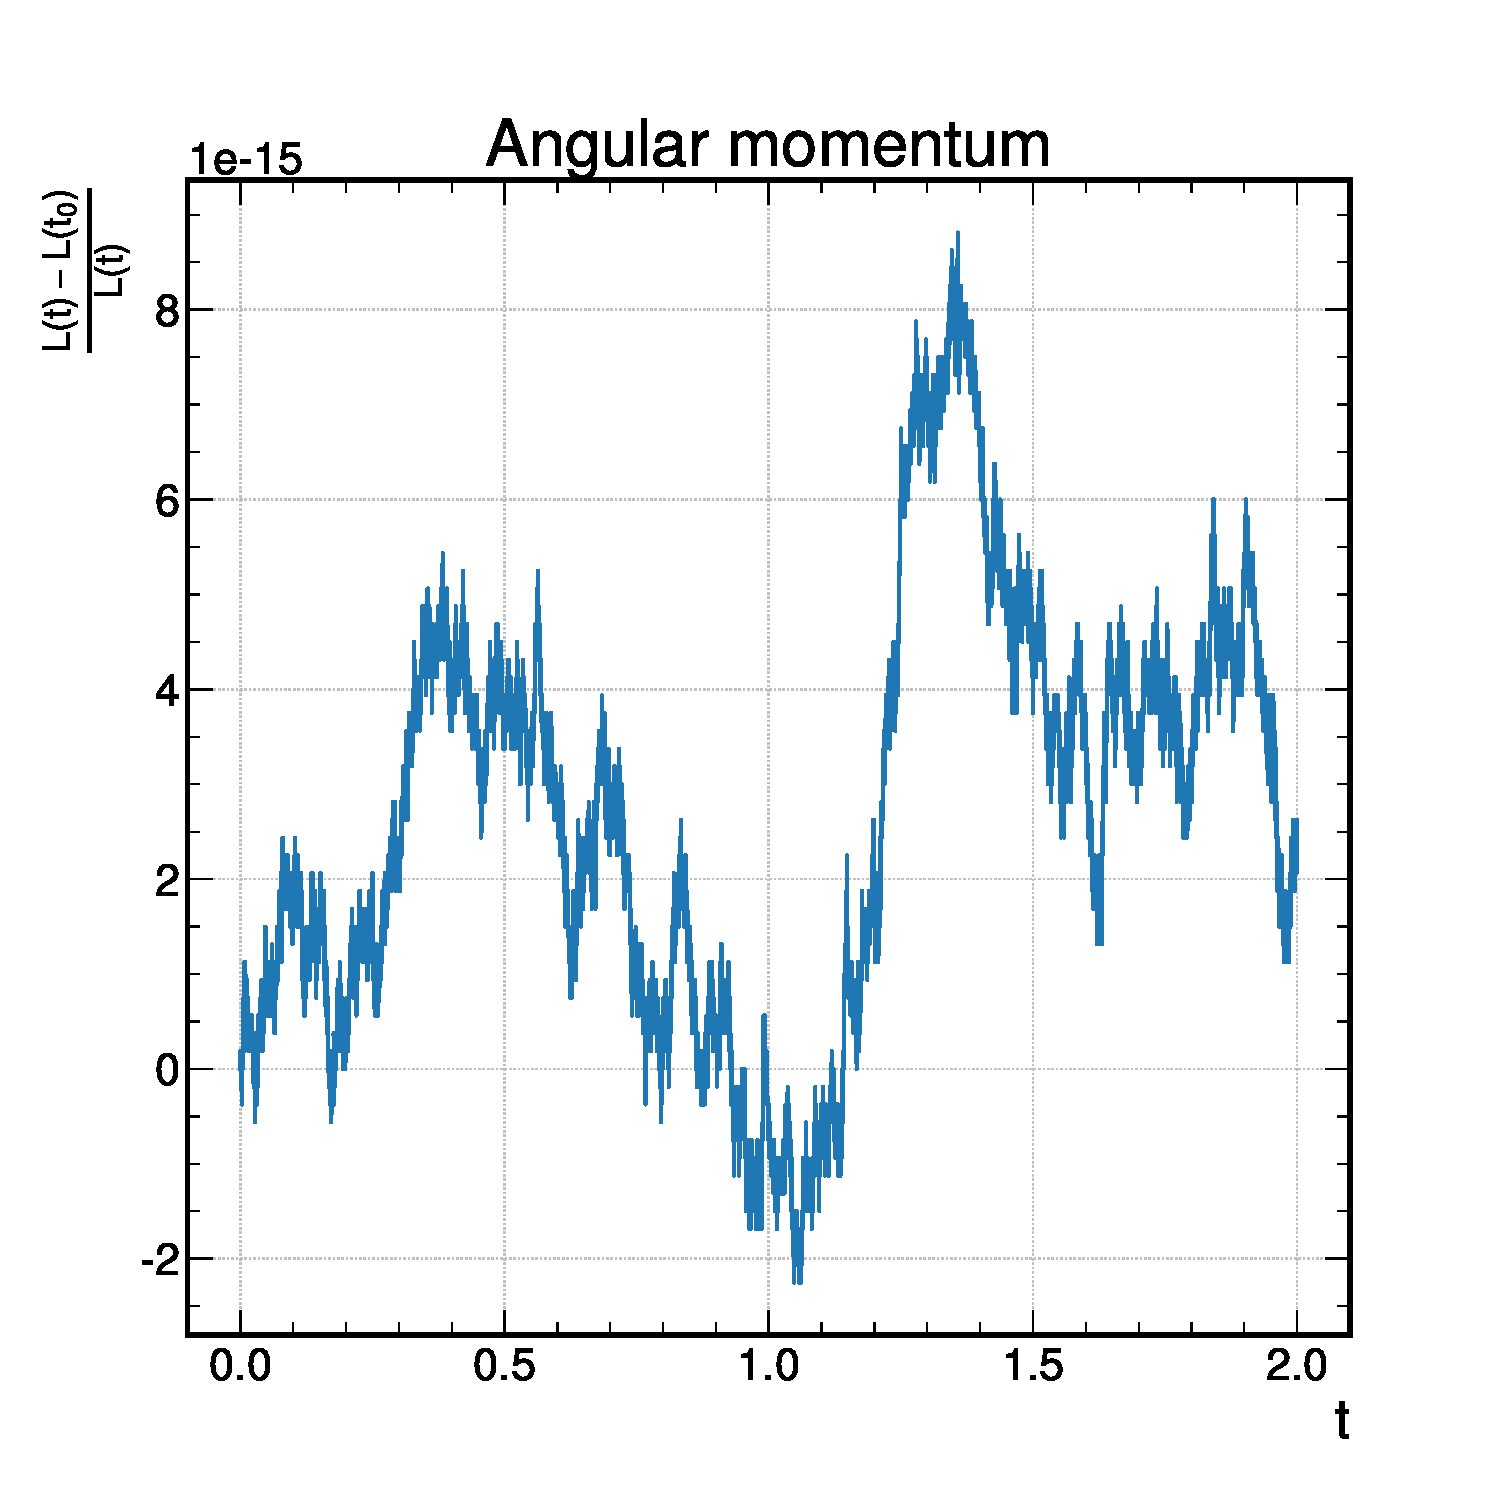
\includegraphics[scale=0.3]{img/ang_euler_simpl.pdf}
\caption{Conservazione di energia e momento angolare con l'integratore di Eulero simplettico.}
\end{figure}
\FloatBarrier

\FloatBarrier
\begin{figure}[h]
\centering
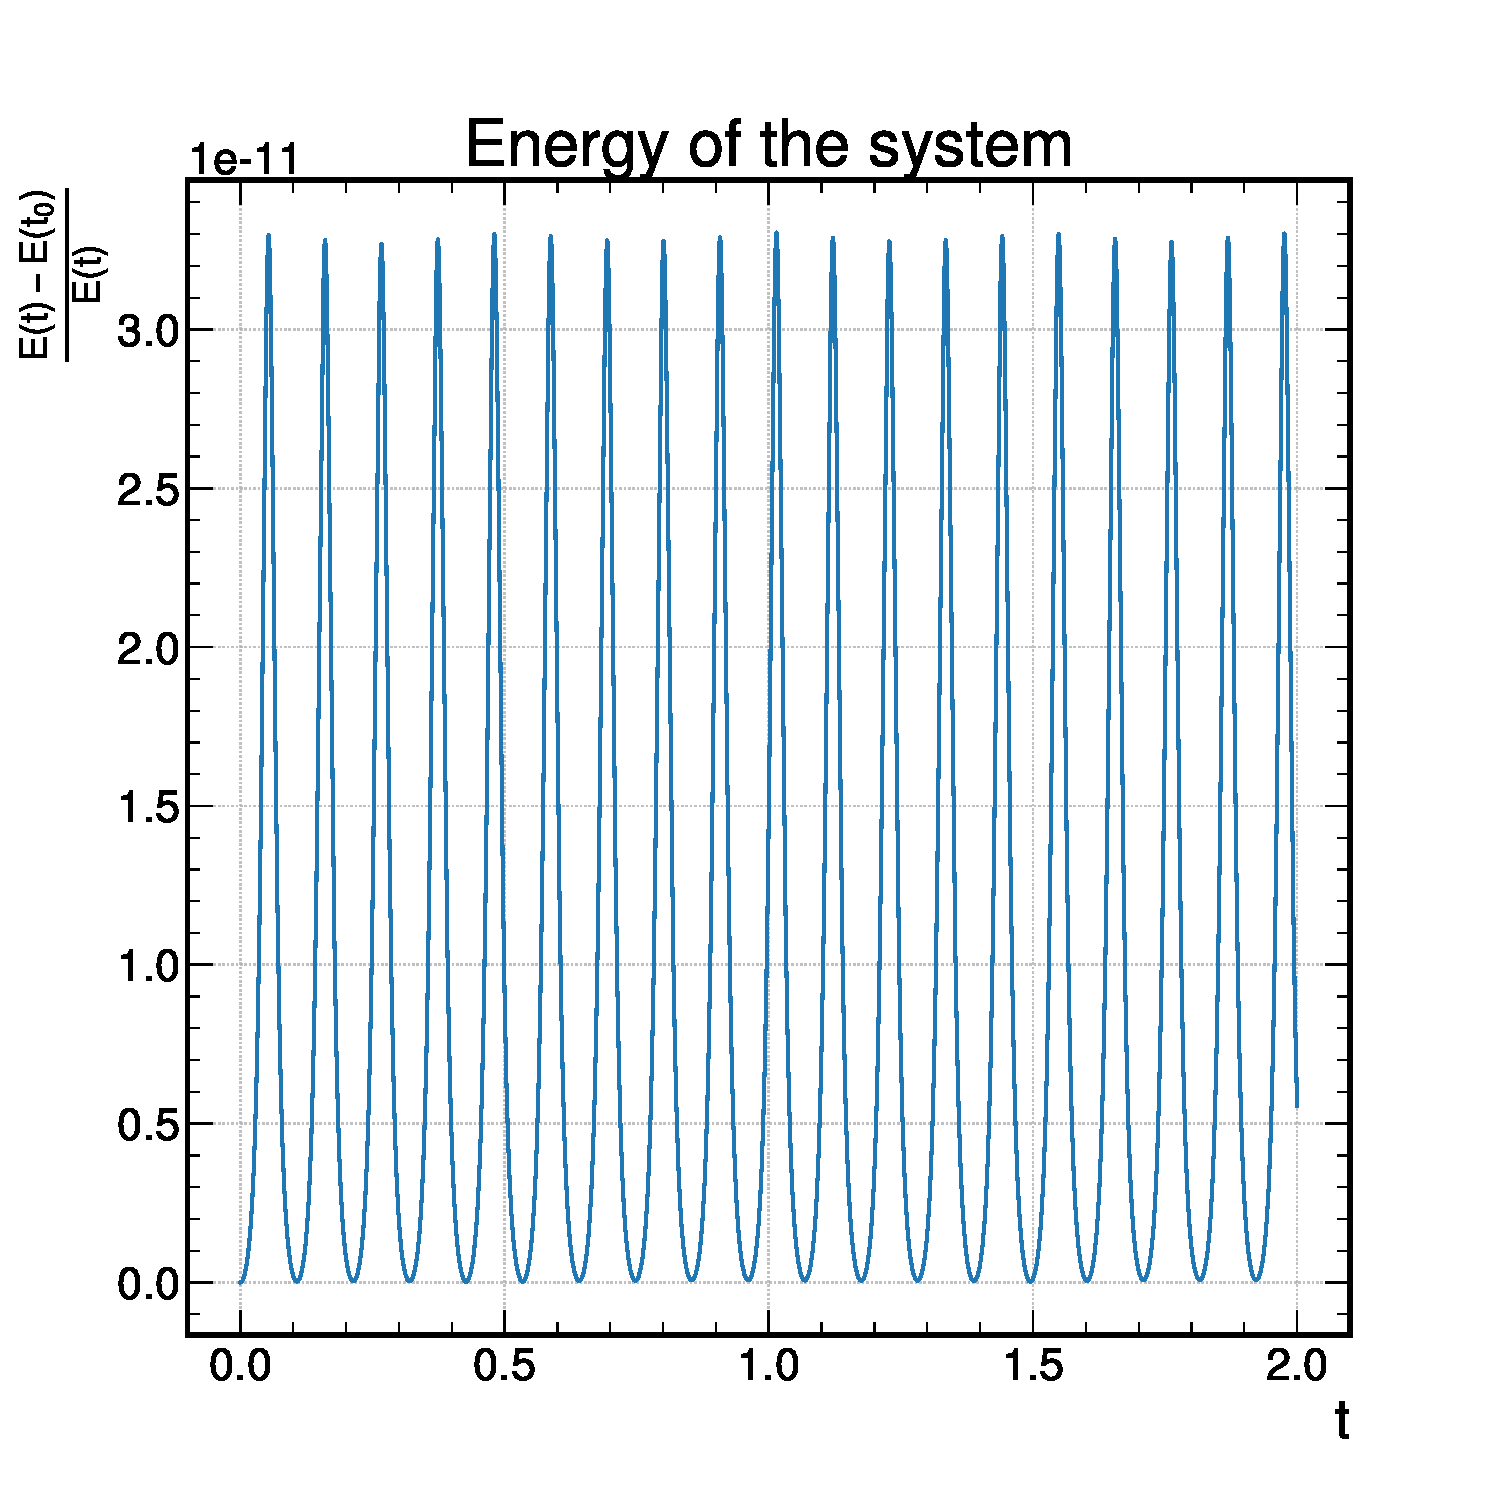
\includegraphics[scale=0.3]{img/ene_yosh_simpl.pdf}
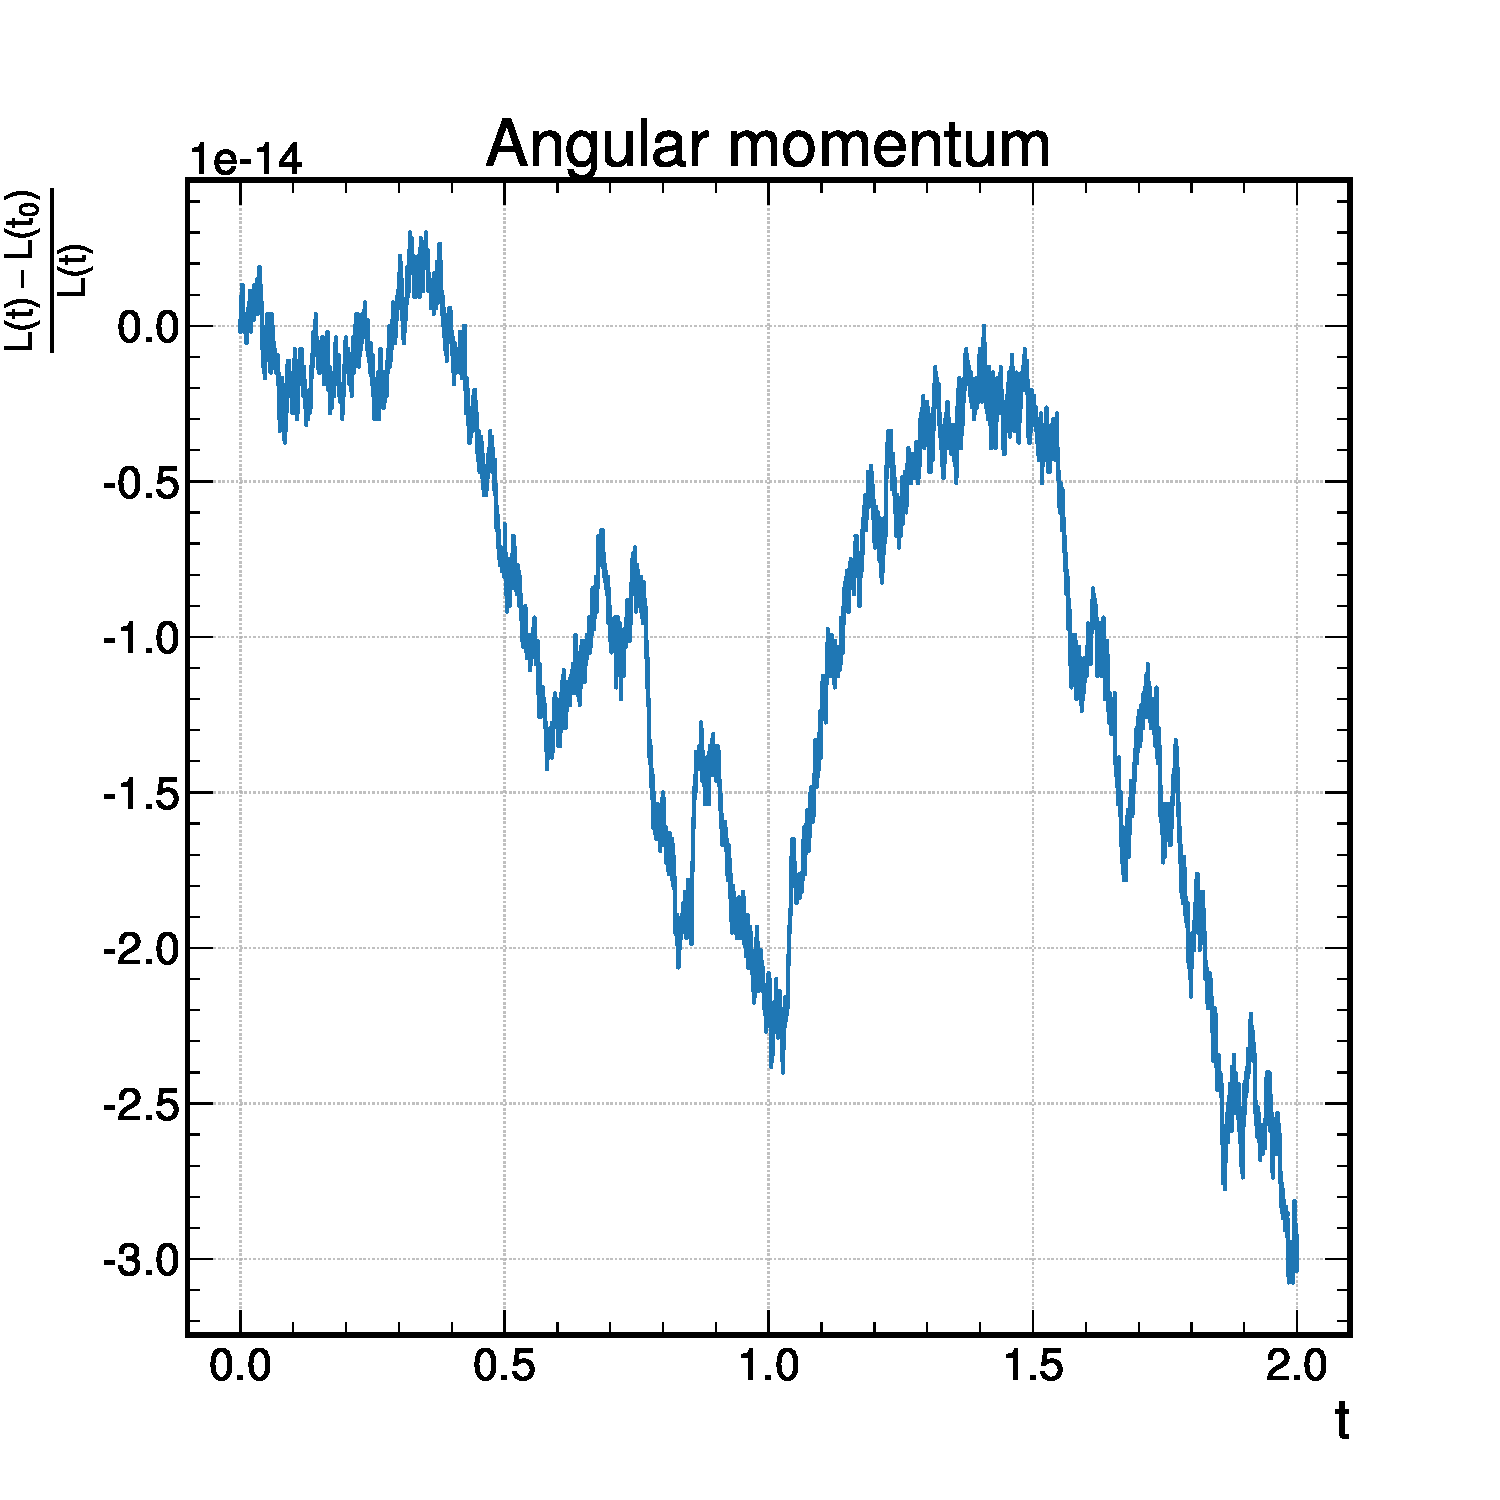
\includegraphics[scale=0.3]{img/ang_yosh_simpl.pdf}
\caption{Conservazione di energia e momento angolare con l'integratore di Yoshida del quarto ordine.}
\end{figure}
\FloatBarrier
Vediamo dunque come la conservazione dell'energia sia molto migliore nel caso di un integratore di ordine superiore, mentre la variazione di momento angolare è sempre dello stesso ordine circa. Avrete notato che lo stile dei plot è leggermente diverso, questo è dovuto al fatto che, per ottenere una migliore leggibilità, si è usato:

\begin{lstlisting}[language=Python]
import mplhep
plt.style.use(mplhep.style.CMS)
\end{lstlisting}
Ok che è pallettaro ma onore al merito.
\subsection{Più che una funzione}
Le classi sono molto utili perché ci permettono di poter fare più cose che una funzione, ma possono anche essere chiamate come una funzione; ad esempio grazie al metodo "\_\_call\_\_" l'istanza che creiamo sarà una funzione. In una delle appendici è presente un codice che esegue un'interpolazione lineare; se andiamo a vederlo e ci fermiamo un attimo a pensare notiamo subito che quella funzione ogni volta che vine chiamata rifà tutto il conto necessario per trovare i coefficienti del polinomio in tutto l'intervallo. Con l'utilizzo di una classe possiamo calcolarci nel costruttore i coefficienti del polinomio e poi chiamare la funzione creata, la quale sa già i coefficienti del polinomio e quindi sarà effettivamente più veloce. Vediamo il caso, un po' più complicato ma più interessante, di una spline cubica (anche se a mali estremi un'interpolazione lineare funziona sempre, ordini più alti possono dare problemi):

\begin{lstlisting}[language=Python]
class CubicSpline:
    '''
    1-D interpolating natural cubic spline
    
    Parameters
    ----------
    xx : 1darray
        value on x must be strictly increasing
    yy : 1darray
        value on y
    
    Example
    -------
    >>>import numpy as np
    >>>import matplotlib.pyplot as plt
    >>>x = np.linspace(0, 1, 10)
    >>>y = np.sin(2*np.pi*x)
    >>>F = CubicSpline(x, y)
    >>>print(F(0.2))
    0.9508316728694627
    
    >>>z = np.linspace(0, 1, 100)
    >>>plt.figure(1)
    >>>plt.title('Spline interpolation')
    >>>plt.xlabel('x')
    >>>plt.ylabel('y')
    >>>plt.plot(z, F(z), 'b', label='Cubic')
    >>>plt.plot(x, y, marker='.', linestyle='', c='k', label='data')
    >>>plt.legend(loc='best')
    >>>plt.grid()
    >>>plt.show()
    '''

    def __init__(self, xx, yy):
    
        self.x = xx                      # x data
        self.y = yy                      # y data will be the constant of polynomial
        self.N = len(xx)                 # len of data     
        alpha  = np.zeros(self.N-1)      # auxiliar array
        self.b = np.zeros(self.N-1)      # linear term
        self.c = np.zeros(self.N)        # quadratic term
        self.d = np.zeros(self.N-1)      # cubic term
        l      = np.zeros(self.N)        # auxiliar array
        z      = np.zeros(self.N)        # auxiliar array
        mu     = np.zeros(self.N)        # auxiliar array
        
        if not np.all(np.diff(xx) > 0.0):
            raise ValueError('x must be strictly increasing')
        
        dx = xx[1:] - xx[:-1]
        a = yy

        for i in range(1, self.N-1):
            alpha[i] = 3*(a[i+1] - a[i])/dx[i] - 3*(a[i] - a[i-1])/dx[i-1]
        
        l[0]  = 1.0
        z[0]  = 0.0
        mu[0] = 0.0
        
        for i in range(1, self.N-1):
            l[i]  = 2.0*(xx[i+1] - xx[i-1]) - dx[i-1]*mu[i-1]
            mu[i] = dx[i]/l[i]
            z[i]  = (alpha[i] - dx[i-1]*z[i-1])/l[i]
          
        l[self.N-1] = 1.0
        z[self.N-1] = 0.0
        self.c[self.N-1] = 0.0
        
        #Coefficient's computation
        for i in range(self.N-2, -1, -1):
            
            self.c[i] = z[i] - mu[i]*self.c[i+1]
            self.b[i] = (a[i+1] - a[i])/dx[i] - dx[i]*(self.c[i+1] + 2.0*self.c[i])/3.0
            self.d[i] = (self.c[i+1] - self.c[i])/(3.0*dx[i])
    
     
    def __call__(self, x):
        '''
        x : float or 1darray
            when we want compute the function
        '''
        n = self.check(x)

        if n == 1 :
            
            for j in range(self.N-1):
                if self.x[j] <= x <= self.x[j+1]:
                    i = j
                    break

            q = (x - self.x[i])
            return self.d[j]*q**3.0 + self.c[j]*q**2.0 + self.b[j]*q + self.y[j]
            
        else:
            F = np.zeros(n)
            for k, x1 in enumerate(x):
                
                for j in range(len(self.x)-1):
                    if self.x[j] <= x1 <= self.x[j+1]:
                        i = j
                        break

                q = (x1 - self.x[i])
                F[k] = self.d[j]*q**3.0 + self.c[j]*q**2.0 + self.b[j]*q + self.y[j]

            return F
        
    
    def check(self, x):
        try :
            n = len(x)
            x_in = np.min(self.x) <= np.min(self.x) and np.max(self.x) >= np.max(x)
        except TypeError:
            n = 1
            x_in = np.min(self.x) <= x <= np.max(self.x)

        # if the value is not in the correct range it is impossible to count
        if not x_in :
            errore = 'Value out of range'
            raise Exception(errore)
        
        return n
if __name__ == '__main__':

    x = np.linspace(0, 1,10)
    y = np.sin(2*np.pi*x)
    
    z = np.linspace(0, 1, 1000)
    G = CubicSpline(x, y)
    
    print(G(0.2))

    plt.figure(1)
    plt.title('Spline interpolation')
    plt.xlabel('x')
    plt.ylabel('y')
    plt.plot(z, G(z), 'r', label='Cubic')
    plt.plot(x, y, marker='.', linestyle='', c='k', label='data')
    plt.legend(loc='best')
    plt.grid()
    plt.show()
    
        
    #==================================================
    # Cfr scipy and our spline
    #==================================================
    
    from scipy.interpolate import InterpolatedUnivariateSpline
    s3 = InterpolatedUnivariateSpline(x, y, k=3)
    plt.figure(2)
    plt.subplot(211)
    plt.title("Spline interpolation N = 10", fontsize=15);
    plt.ylabel("error", fontsize=15)
    plt.plot(z, G(z)-np.sin(2*np.pi*z), 'b', label='CubicSpline');
    plt.plot(z, s3(z)-np.sin(2*np.pi*z), 'r', label='Scipy');
    plt.grid();plt.legend(loc='best');
    plt.subplot(212);
    plt.title("Spline interpolation N = 30", fontsize=15)
    
    x = np.linspace(0, 1, 30)
    y = np.sin(2*np.pi*x)
    G = CubicSpline(x, y)
    s3 = InterpolatedUnivariateSpline(x, y, k=3)
    
    plt.ylabel("error", fontsize=15)
    plt.xlabel('x', fontsize=15)
    plt.plot(z, G(z)-np.sin(2*np.pi*z), 'b', label='CubicSpline');
    plt.plot(z, s3(z)-np.sin(2*np.pi*z), 'r', label='Scipy');
    plt.grid();plt.legend(loc='best')
    plt.show()

[Output]
0.9508316728694627
\end{lstlisting}
Fondamentalmente che succede: noi creiamo G, istanza della classe CubicSpline, nel farlo chiamiamo il costruttore il quale calcola i coefficienti dei polinomi interpolanti. Ora però grazie al metodo "\_\_call\_\_" G è un oggetto chiamabile. Avete presente quando in altri codici passando funzioni ad altre funzioni nella documentazione scrivevamo callable? Ecco è proprio questo, è come se la vostra funzione fosse il metodo "\_\_call\_\_" della classe. Quindi chiamando l'istanza viene eseguito il metodo "\_\_call\_\_" il quale, nel nostro caso, sa già i dati necessari e sa calcolarci la spline. Giusto per completezza precisiamo che questa spline cubica non è esattamente la stessa spline cubica di scipy che abbiamo visto sopra; questa si chiama spline naturale e ai bordi si comporta un pò diversamente rispetto a scipy (meglio anche). Per vederlo calcoliamo la differenza fra l'interpolazione calcolata in $z$ (l'array nel codice) e i valori che restituisce "np.sin(2*np.pi*z)"; Facciamo due casi, interpoliamo prima $10$ e poi $30$ punti. Il codice sopra mostrato è riportato nella cartella interpolazioni, benché mostrato in questa sezione. Inoltre è riportato la stessa implementazione per il caso lineare.

\begin{center}
\makebox[\textwidth][c]{
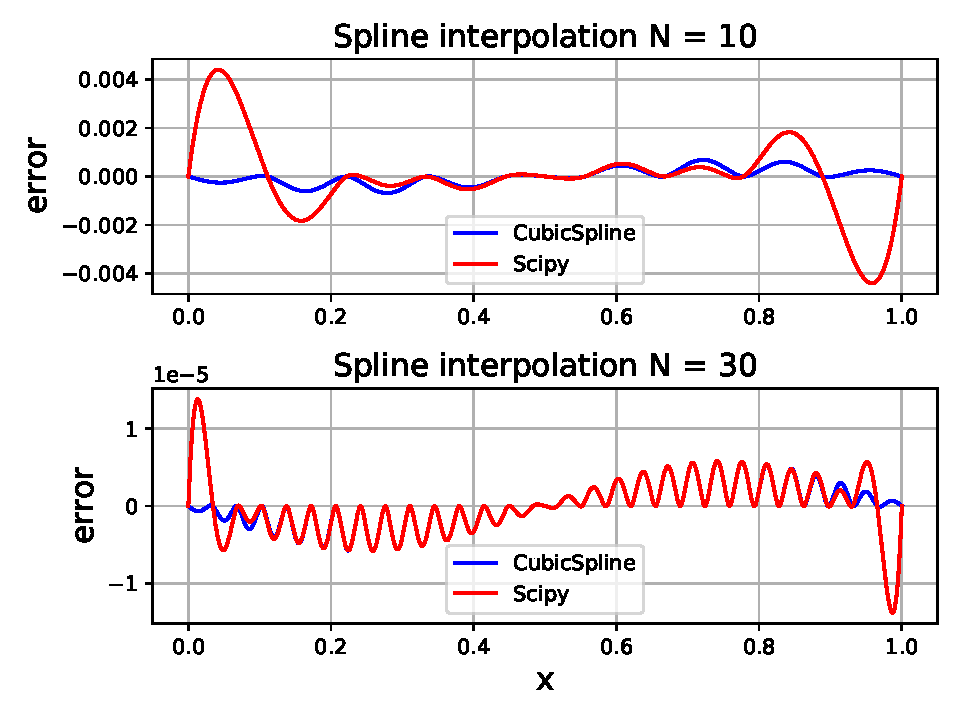
\includegraphics[scale=0.9]{img/cfr_spline.pdf}
}
\end{center}

\newpage

\section{Quarta Lezione A}
\subsection{Reti neurali}
Essendo il computer molto stupido a qualcuno è venuta la brillante idea di cercare di educarlo, tanto per divertirsi un po'. Cominciamo quindi questa \emph{descensio ad inferos} di cui al più faremo i primi gradini. Vogliamo infatti costruire un semplice esempio di rete neurale, che serva a classificare dei dati. Quello che vogliamo fare è costruire una scatola nera che prenda in input un certo set di dati a cui corrisponde un certo label, e la nostra scatola nera deve imparare a capire qual è il label a seconda di varie caratteristiche presenti nei dati in input. Metaforicamente potremmo dire che "allenare" una rete neurale è come fare esercizi guardando le soluzioni finché non diventi bravo e impari a farli da solo. Si tratta quindi di apprendimento supervisionato. Vediamo uno schema di una rete neurale e cerchiamo di capire cosa succede.
\FloatBarrier
\begin{figure}[h]
\centering
\begin{neuralnetwork}[height=4]
\newcommand{\x}[2]{$x_#2$}
\newcommand{\y}[2]{$\hat{y}_#2$}
\newcommand{\hfirst}[2]{\small $f^{(1)}_#2$}
\newcommand{\hsecond}[2]{\small $f^{(2)}_#2$}
\inputlayer[count=2,  bias=false,  title=Input\\layer, text=\x]
\hiddenlayer[count=4, bias=false, title=Hidden\\layer 1, text=\hfirst] \linklayers
\hiddenlayer[count=4, bias=false, title=Hidden\\layer 2, text=\hsecond] \linklayers
\outputlayer[count=1, title=Output\\layer, text=\y] \linklayers
\end{neuralnetwork}
\caption{Schema di una rete neurale per una classificazione binaria, eventualmente il layer di output può avere due neuroni in caso di one-hot-encoding}
\end{figure}
\FloatBarrier
Questo è un piccolo esempio della struttura di una rete neurale. Essa è suddivisa in layer e ogni layer contiene un certo numero di neuroni (i pallini). Il layer di input è quello a cui noi passiamo i dati, mentre il layer di output è quello che ci restituisce il risultato; è negli hidden layer che avviene la magia. Supponiamo di avere dei dati del tipo:
\FloatBarrier
\begin{table}[h]
\centering
\begin{tabular}{ccc}
\hline
$x_1$ & $x_2$ & $y$ \\
\hline 
0.34 & 0.56 & 1 \\ 
0.5 & 0.89 & 1 \\ 
0.2 & 0.7 & 0 \\ 
0.52 & 0.1 & 1 \\ 
0.9 & 0.83 & 0 \\ 
$\vdots$ & $\vdots$ & $\vdots$ \\
\hline 
\end{tabular}
\caption{Tabella di dati da classificare: ogni dato ha due features ovvero le due coordinate $x_1$ e $x_2$ ed un label o target ovvero $y$, cioè abbiamo assegnato ad ogni punto sul piano un valore binario 0 o 1.}
\end{table}
\FloatBarrier
Quindi abbiamo dei punti sul piano, senza perdere di generalità supponiamoli fra 0 ed 1, e li abbiamo targhettati con uno zero o con un uno. Vediamo ora come addestrare la rete. Come prima cosa passiamo i dati in input alla rete e facciamo il primo passo, cioè dobbiamo andare verso il primo layer nascosto, quello che in genere si fa è la seguente cosa:
\begin{equation}
\textbf{z} = W \textbf{x} + \textbf{b} \quad.
\end{equation}
Non molto magico eh? vediamo gli elementi di questa formula $\textbf{x}$ è il vettore in input quindi $\textbf{x} = (x_1, x_2)$; $W$ è una matrice e gli elementi vengono chiamati pesi; infine $\textbf{b}$ è un vettore ed è chiamato bias. Le dimensioni di questa matrice e questo vettore sono dati dalla dimensione del layer: nella fattispecie per il primo layer $W$ sarà una matrice $4 \times 2$ e $\textbf{b}$ un vettore lungo 4. Per cui anche il nostro output $\textbf{z}$ sarà un vettore lungo 4. Più in generale possiamo dire, essendo questa struttura la stessa per ogni layer, che la dimensione di $W$ sarà sempre della forma: (numero di neuroni nel layer attuale)$\times$(numero di neuroni layer precedente), mentre $\textbf{b}$ sarà sempre un vettore lungo (numero di neuroni nel layer attuale). La domanda sorge spontanea: che valori hanno le entrate di $W$ e di $\textbf{b}$? Inizialmente saranno scelte in maniera casuale e poi vedremo che durante le iterazioni di allenamento, dette epoche, esse verranno aggiornate secondo una certa regola. Prima di passare al secondo layer però c'è un'altra operazione da fare. Infatti solitamente non è $\textbf{z}$ l'output ma $f(\textbf{z})$ dove $f$ è una certa funzione $f : \mathbb{R} \to \mathbb{R}$. Questa $f$ è chiamata funzione di attivazione del neurone; essa restituirà nel nostro caso un vettore lungo 4 che sarà l'input per il layer successivo. Possiamo vedere tutto ciò come delle regole per far accendere o spegnere un neurone. Fatto questo il procedimento si ripete in maniera uguale per ogni layer fino ad arrivare al layer di output. Ora che il passaggio attraverso la rete è stato fatto dobbiamo capire se l'output che genera la rete è simile a quello che noi vogliamo. \' E dunque arrivato il momento di calcolare una funzione che misuri la distanza tra risultato esatto e risultato della rete. Questa funzione è chiamata \textit{loss} e nel nostro caso di classificazione binaria useremo quella che è chiamata binary cross entropy:
\begin{equation}
\mathcal{L} = \frac{1}{N} \sum_i^N (y_i \log(\hat{y}_i) + (1 - y_i) \log(1 - \hat{y}_i)) \quad.
\end{equation}
Non vi sarà sfuggito il fatto che questa è la classica espressione per l'entropia di un sistema di fermioni. Precisiamo che $N$ è il numero di dati che passiamo per farlo allenare (volendo il numero di righe della tabella di sopra).
Fatto questo non ci resta che decidere il modo il cui aggiornare i pesi e bias della rete. Abbiamo detto che la loss misura la distanza di quanto la rete sbaglia, quindi basterà minimizzarla. Trovando il punto di minimo avremo i parametri (pesi e bias) ottimali della nostra rete. Come se stessimo eseguendo un fit, circa. Per farlo usiamo il più semplice e classico algoritmo: il gradiente discendente (di cui è presente una discussione in una delle appendici). Abbiamo quindi che:
\begin{align}
W^{i+1} &= W^i - \alpha \frac{\partial \mathcal{L}}{\partial W^i} , \\
\textbf{b}^{i+1} &= \textbf{b}^{i} - \alpha \frac{\partial \mathcal{L}}{\partial \textbf{b}^i},
\end{align}
dove $\alpha$ è chiamato "learning rate" ed è un parametro che scegliamo noi. Immagino non vi sorprenderà sapere che le derivate copra citate si calcolano con la chain rule:
\begin{align}
\frac{\partial \mathcal{L}}{\partial W} &= \frac{\partial \mathcal{L}}{\partial \hat{y}} \, \frac{\partial f}{\partial z} \, \frac{\partial (W \textbf{x} + \textbf{b})}{\partial W}, \\
\frac{\partial \mathcal{L}}{\partial \textbf{b}} &= \frac{\partial \mathcal{L}}{\partial \hat{y}} \, \frac{\partial f}{\partial z} \, \frac{\partial (W \textbf{x} + \textbf{b})}{\partial \textbf{b}}.
\end{align}
Fatto questo abbiamo dei nuovi pesi e bias con cui ripartire prendendo nuovamente i dati in input e propagarli lungo la rete. Questo passaggio si chiama "feed forward" mentre l'updating è chiamato "backpropagation". Fatti questi, è finita un'iterazione, ovvero un epoca, e parte la successiva. Il numero di epoche è anch'esso un parametro che scegliamo noi. Altra cosa che sta al nostro giudizio è la scelta delle funzioni di attivazione, per le quali, eccezion fatta per il layer di output, non ci sono chissà che criteri per selezionarle. In letteratura si possono trovare le scelte più disparate. Noi useremo per tutti i layer nascosti delle tangenti iperboliche e per il layer di output una sigmoide.
Aggiungiamo altre due cose: avendo usato come loss la binary cross entropy può essere interessante misurare l'accuratezza del risultato della rete anche in un altro modo, calcoliamo:
\begin{equation}
a = 1 - \Bigg| \sum_i^N \frac{\hat{y}_i - y_i}{N} \Bigg| ,
\end{equation}
detta accuratezza più siamo vicini ad uno meglio è però bisogna stare attenti a non overfittare. La rete potrebbe infatti star "imparando a memoria" e questo non va bene. Per controllare che questo non succeda usiamo quella è chiamata validation loss. Si tratta sempre di calcolare la loss, ma non sui dati che usiamo come dati di allenamento, ma su un altro set che usiamo esclusivamente per questo calcolo. Quindi noi passiamo alla rete dei dati e li dividiamo in due, su un set allena e sull'altro valida. Quello che facciamo è plottare insieme la loss calcolata sui dati di allenamento e quella calcolata sui dati di validation (in funzione delle epoche). Se le due scendono insieme la rete si sta comportando bene. Se invece ad un certo punto la loss scende ma la loss di validation sale vuol dire che la rete sta overfittando, cioè sta imparando a memoria le caratteristiche dei dati di allenamento. Quindi per evitare questo bisogna scegliere alcuni parametri con un po' di senno, ad esempio learning rate, numero di neuroni e numero di layer o anche numero di epoche. 
Detto questo passiamo ora a vedere il codice. Implementeremo una rete neurale con un solo layer nascosto con numero di neuroni variabile, due neuroni in input e uno solo in output. Lo scopo sarà proprio di riconoscere dati dei punti nel quadrato $[0, 1] \times [0, 1]$ se essi hanno un valore associato 1 oppure 0. L'inizializzazione verrà fatta estraendo dei numeri distribuiti gaussianamente. Omettiamo per brevità, come sempre, le funzioni che fanno i plot e quello che è il main del codice.
\begin{lstlisting}[language=Python]
"""
Code that implement a shallow neural network for a binary classifications.
The code is witten imposed 2 imput, 1 output e one hidden layer.
Is possible to choose the dimesions of hidden layer.
It is also possible to save plots during the run to see how the network is learning.
"""
import numpy as np
import matplotlib.pyplot as plt

#=============================================================
# Loss function binary classification
#=============================================================

def Loss(Yp, Y):
    '''
    loss function, binary crosss entropy
    
    Parameters
    ----------
    Yp : 1darray
        actual prediction
    Y : 1darray
        Target
    
    Returns
    -------
    float, binary crosss entropy
    '''
    m = len(Y)
    return -np.sum(Y*np.log(Yp) + (1 - Y)*np.log(1 - Yp))/m

#=============================================================
# Activation function
#=============================================================

# Hidden layer
def g1(x):
    return np.tanh(x)
# Output layer
def g2(x):
    return 1 / (1 + np.exp(-x))

#=============================================================
# Initialization
#=============================================================

def init(n):
    '''
    Random initialization of parameters weights and biases
    
    Parameters
    ----------
    n : int
        number of neurons in the hidden layer
    
    Returns
    -------
    W1, b1 : 2darray
        weights and bias for hidden layer
    W2, b2 : 2darray
        weights and bias for output layer
    '''
    # Hidden layer
    # nx2 because 2 featurs and n neurons
    W1 = np.random.randn(n, 2)
    b1 = np.random.rand(n, 1)
    # Output layer
    # 1xn because 1 output and n neurons
    W2 = np.random.randn(1, n)
    b2 = np.random.rand(1, 1)
    return W1, b1, W2, b2

#=============================================================
# Network prediction function
#=============================================================

def predict(X, W1, b1, W2, b2):
    """
    Function that returns the prediction of the network
    
    Parameters
    ----------
    X : 2darray
        data, featurs
    W1, b1, W2, b2 : 2darray
        parameter of the network
    
    Returns
    -------
    A1 : 1d array
        intermediate prediction
    A2 : 1d array
        final prediction
    """
    # Hidden layer
    Z1 = W1 @ X + b1
    A1 = g1(Z1)
    # Output layer
    Z2 = W2 @ A1 + b2
    A2 = g2(Z2)
    
    return A1, A2

#=============================================================
# Backpropagation function
#=============================================================

def backpropagation(X, Y, step, A1, A2, W1, b1, W2, b2):
    '''
    Backpropagation function.
    Update weights and biases with gradient descendent
    all the quantities came from taking the derivative of the Loss
    
    Y : 1darray
        Target
    step : float
        learning rate
    A1, A2 : 1darray
        predictions of the network
    W1, b1, W2, b2 : 2darray
        parameter of the network
    '''
    m = len(Y)
    # Output layer 
    dLdZ2 = (A2 - Y)
    dLdW2 = dLdZ2 @ A1.T / m
    dLdb2 = np.sum(dLdZ2, axis=1)[:, None] / m
    # Hidden layer
    dLdZ1 = W2.T @ dLdZ2 * (1 - A1**2)
    dLdW1 = dLdZ1 @ X.T / m
    dLdb1 = np.sum(dLdZ1, axis=1)[:, None] / m
    
    # Update of parameters
    W1 -= step * dLdW1
    b1 -= step * dLdb1
    W2 -= step * dLdW2
    b2 -= step * dLdb2
    
    return W1, b1, W2, b2

#=============================================================
# Accuracy mesuraments
#=============================================================

def accuracy(Yp, Y):
    '''
    accuracy of prediction. We use:
    accuracy = 1 - | sum ( prediction - target )/target_size |
    
    Parameters
    ----------
    Yp : 1darray
        actual prediction
    Y : 1darray
        Target
    
    Returns
    -------
    a : float
        accuracy
    '''
    m = len(Y)
    a = 1 - abs(np.sum(Yp.ravel() - Y)/m)
    return a
    
#=============================================================
# Train of the network
#=============================================================

def train(X, Y, n_epoch, neuro, step, sp=False, verbose=True):
    '''
    function for the training of the network
    
    Parameters
    ----------
    X : 2darray
        data, featurs
    Y : 1darray
        Target
    n_epoch : int
        number of epoch
    neuro : int
        number of neurons in the hidden layer
    step : float
        learning rate
    sp : boolean, optional, default False
        if True a plot of boundary is saved each 100 epoch
        usefull for animations 
    verbose : boolean, optional, default True
        if True print loss and accuracy each 100 epoch
    
    Returns
    -------
    result : dict
        params -> W1, b1, W2, b2 weights and bias of network
        train_Loss -> loss on train data
        valid_Loss -> loss on validation data
    '''

    W1, b1, W2, b2 = init(neuro)
    L_t = np.zeros(n_epoch) # training loss
    L_v = np.zeros(n_epoch) # validation loss
    N = X.shape[1]          # total number of data
    M = N//4                # nuber of data for validation
     
    # split dataset in validation and train 
    X_train, Y_train = X[:, :N-M ], Y[:N-M ] 
    X_valid, Y_valid = X[:,  N-M:], Y[ N-M:]
    
    for i in range(n_epoch):
        # train
        A1, A2 = predict(X_train, W1, b1, W2, b2)
        L_t[i] = Loss(A2, Y_train)
        # validation
        _, Yp = predict(X_valid, W1, b1, W2, b2)
        L_v[i] = Loss(Yp, Y_valid)
        # update
        W1, b1, W2, b2 = backpropagation(X_train, Y_train, step, A1, A2, W1, b1, W2, b2)
              
        if not i % 100:
            #if sp : plot(X_train, Y_train, (W1, b1, W2, b2), i)
            
            if verbose:
                acc = accuracy(A2, Y_train)
                print(f'Loss = {L_t[i]:.5f}, accuracy = {acc:.5f}, epoch = {i} \r', end='')
            
    if verbose: print()
    
    result = {'params'     : (W1, b1, W2, b2),
              'train_Loss' : L_t,
              'valid_Loss' : L_v,
             }
        
    return result
\end{lstlisting}
Dopo queste belle tre paginate di codice vediamo un po' di risultati. Questo codice era scritto per far vedere come rete impara creando un gif, che trovate disponibile sulla cartella. Il risultato finale è il seguente:
\FloatBarrier
\begin{figure}[h]
\centering
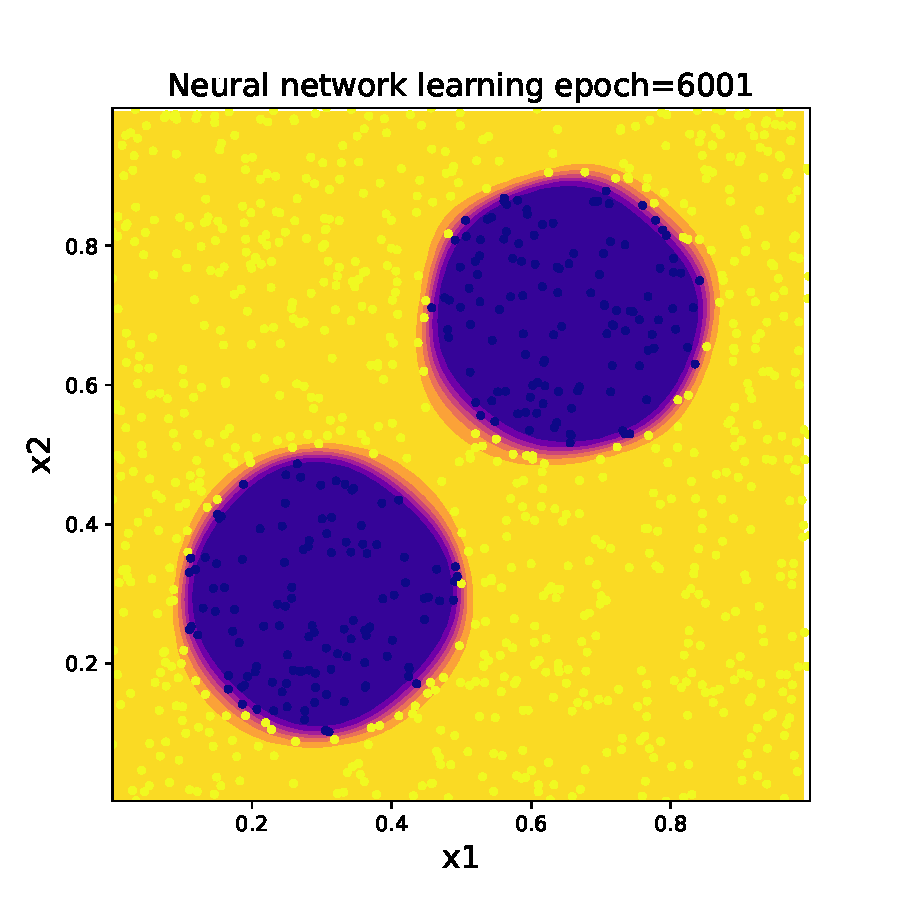
\includegraphics[scale=0.5]{img/6001.pdf}
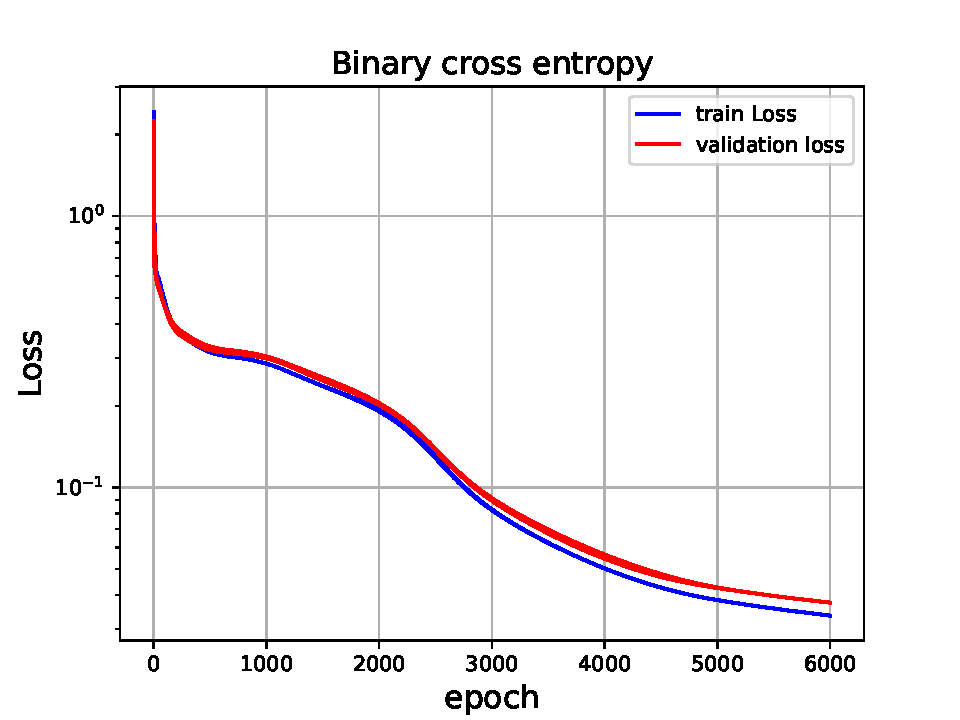
\includegraphics[scale=0.5]{img/Loss1.pdf}
\caption{Risultati della rete neurale, predizione e andamento della loss. I parametri qui sono: 20 neuroni nel layer nascosto, un learning rate di 1.5, 6001 epoche, 3000 dati di train e 1000 di validation.}
\end{figure}
\FloatBarrier
Il plot a sinistra è fatto sui dati di test, quindi un set di dati che la rete non ha usato per allenarsi e il risultato sembra soddisfacente, vediamo poi che le due loss scendono insieme il che è segno che la rete si comporta bene. Volendo ora farvi vedere andamenti diversi della loss vi mostro due grafici provenienti da un altro codice, in cui ho implementato una rete neurale in maniera leggermente diversa e un po' più generale. Anche perché, se vedete la loss nella figura sopra, noterete che la linea è un po' spessa, dovuto al fatto che sta oscillando (immagino sia una concausa tra problema da affrontare e algoritmo di minimizzazione). Il problema è questa volta il MNIST, ovvero il riconoscimento di cifre scritte a mano in bassa risoluzione, ogni immagine è 28$\times$28 pixel. Vediamo un caso in cui la rete overfitta e un caso in cui si comporta bene:
\FloatBarrier
\begin{figure}[h]
\centering
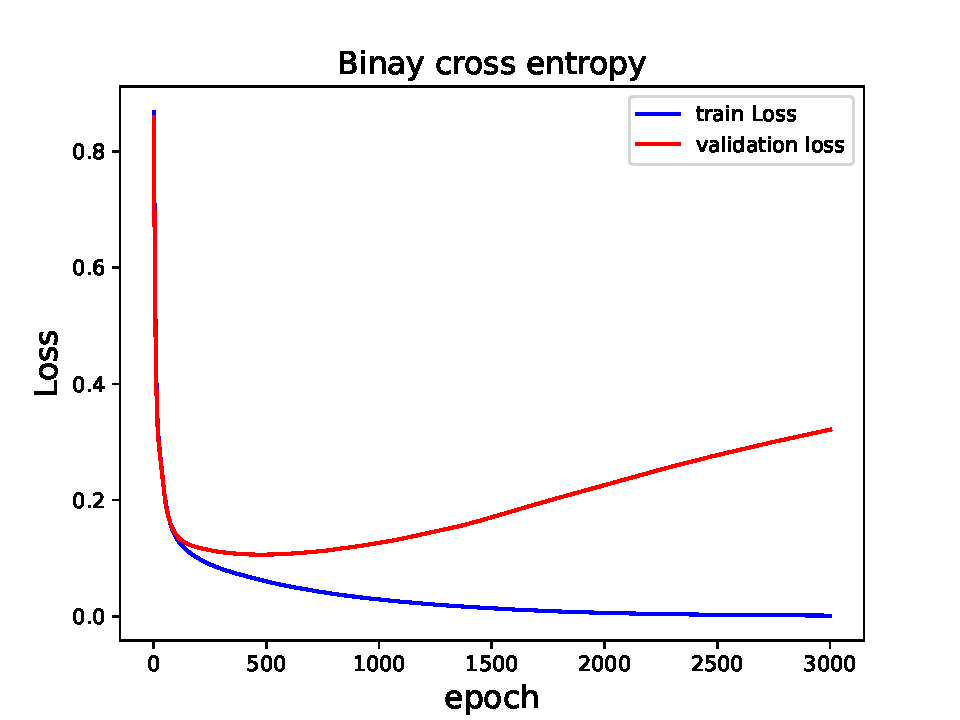
\includegraphics[scale=0.5]{img/Loss_over.pdf}
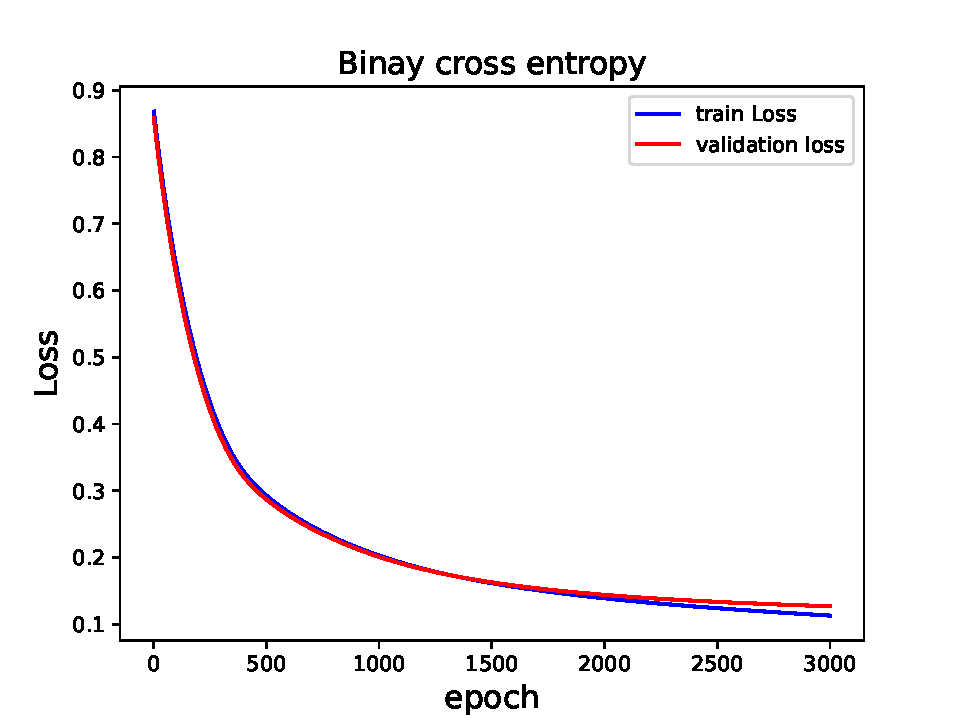
\includegraphics[scale=0.5]{img/Loss_fit.pdf}
\caption{Andamento della loss in funzione delle epoche. Nel grafico a sinistra la rete sta overfittando, mentre a destra l'allenamento procede bene. I parametri qui sono: 2 layer nascosti ognuno da 50 neuroni; l'ottimizzatore usato è ADAM e il learning rate iniziale è di 0.05 per il caso di overfit e di 0.01 per quello di buon fit; le funzioni di attivazione sono: per i leayer nascosti le "relu", mentre una sigmoide per il layer finale. Le epoche sono 3001, 2250 i dati di train e 750 quelli di validation.}
\end{figure}
\FloatBarrier
Vediamo quindi che anche solo il cambiamento del learning rate iniziale (dove si specifica iniziale in quanto ADAM è un algoritmo adattivo) provoca un comportamento che non vogliamo, facendo overfittare la rete. Questo lo possiamo vedere anche, trattandosi di un classificatore, grazie a quelle che sono le matrici di confusione. Mostriamo di seguito le matrici nel caso di overfit e di fit facendo anche il confronto vedendo i dati train e quelli di test. Spieghiamo velocemente come si legge questa matrice: sull'asse delle ordinate è presente la predizione della rete mentre su quello delle ascisse ci sta il risultato esatto. Le entrate di questa matrice ci dicono fondamentalmente quante volte la rete ha detto "x" e doveva dire "y"; quindi gli elementi sulla diagonale sono le risposte esatte mentre i termini fuori sono risposte sbagliate. Per chiarezza precisiamo che questa matrice viene calcolata sempre a fine allenamento.
\FloatBarrier
\begin{figure}[h]
\centering
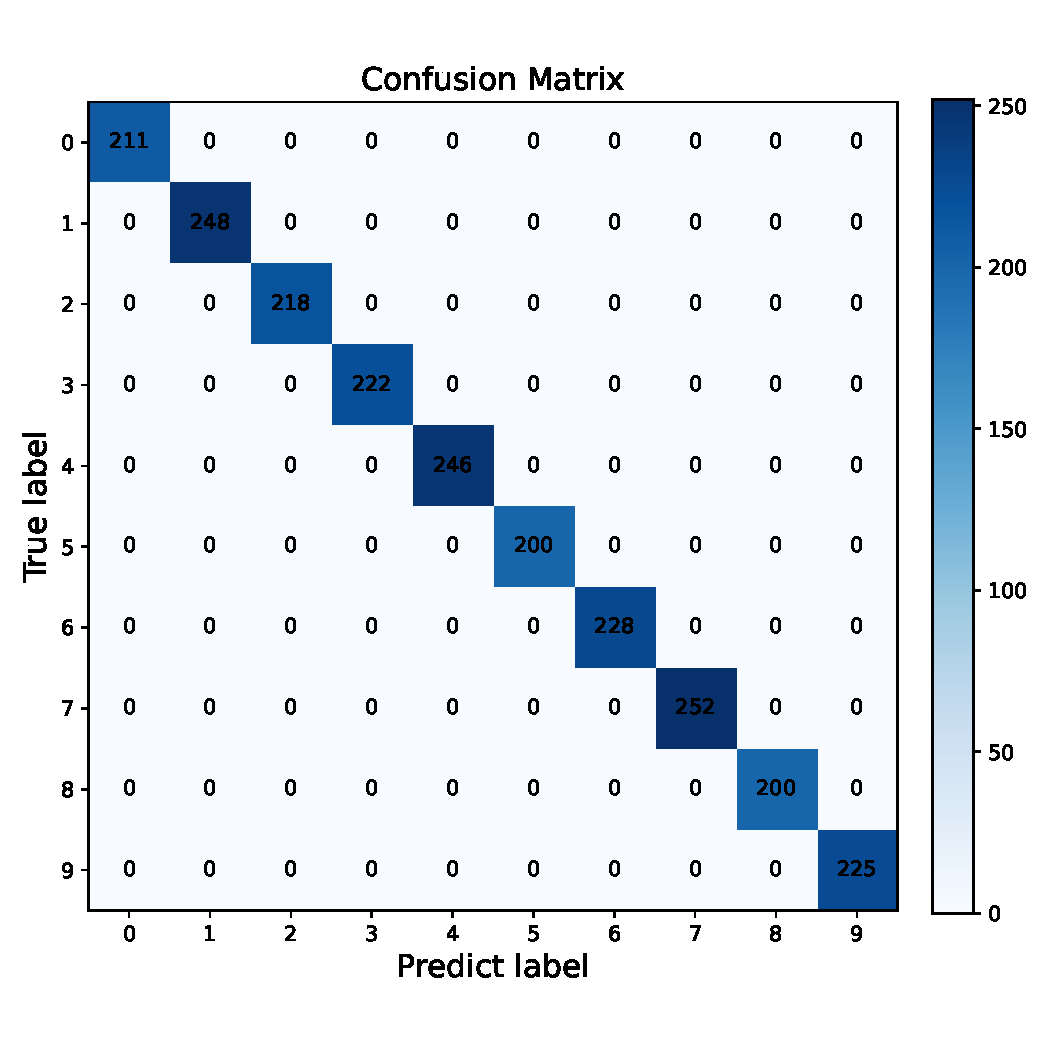
\includegraphics[scale=0.4]{img/conf_mat_over_train.pdf}
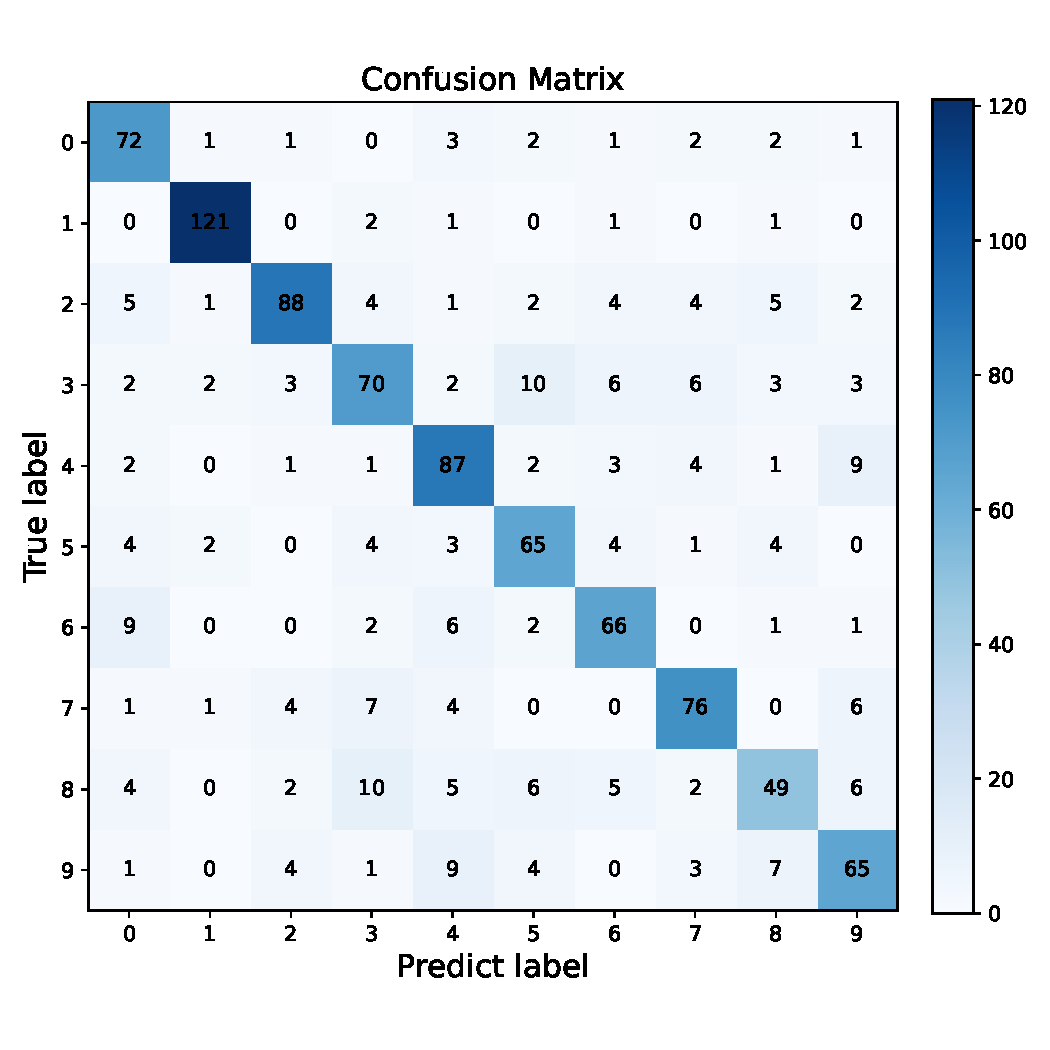
\includegraphics[scale=0.4]{img/conf_mat_over_test.pdf}
\caption{Vediamo qui le matrici nel caso di overfit calcolate sui dati di train, a sinistra, e su quelli di test, a destra. Avendo imparato a memoria le caratteristiche dei dati di train vediamo effettivamente che la rete non sbaglia una singola predizione. Mentre a destra, su dati che per la rete sono nuovi, ci sono molti più errori.}
\end{figure}
\FloatBarrier
\FloatBarrier
\begin{figure}[h]
\centering
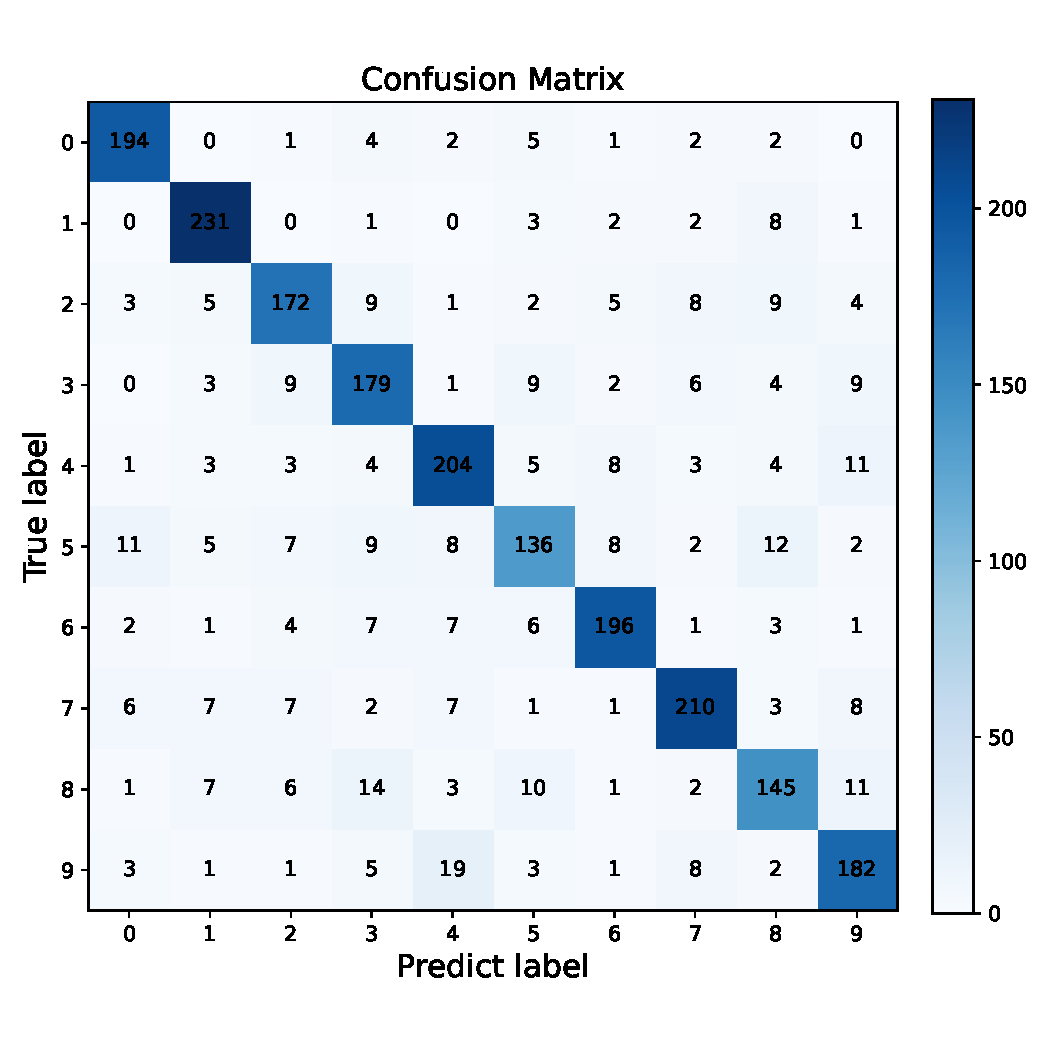
\includegraphics[scale=0.4]{img/conf_mat_fit_train.pdf}
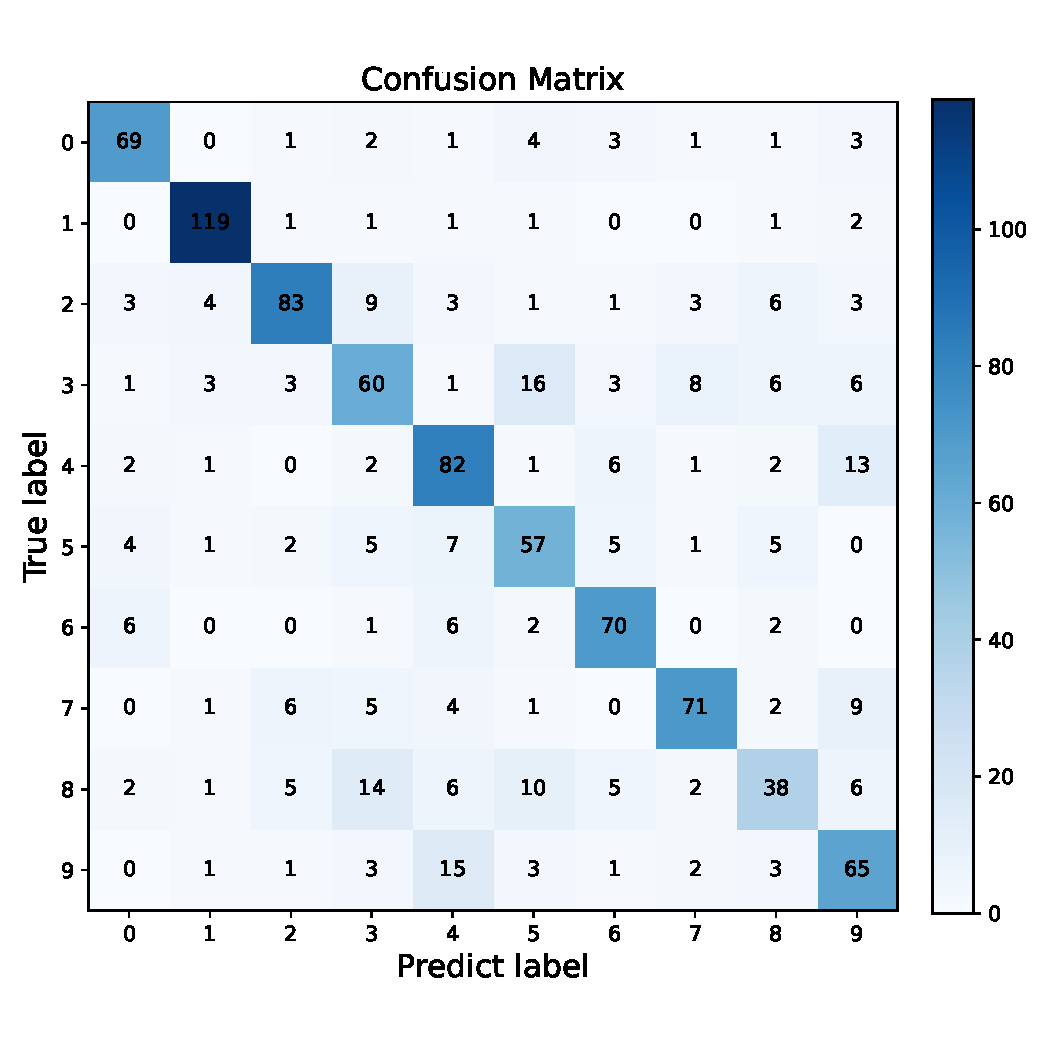
\includegraphics[scale=0.4]{img/conf_mat_fit_test.pdf}
\caption{Vediamo qui le matrici nel caso di buon fit calcolate sui dati di train, a sinistra, e su quelli di test, a destra. Questa volta la rete non ha imparato a memoria, vediamo infatti che ci sono risposte sbagliate un po' ovunque. Le due matrici sembrano parenti.}
\end{figure}
\FloatBarrier
Per concludere questa discussione in caso fosse di vostro interesse vi mostro il codice per calcolare queste matrici di confusione:


\begin{lstlisting}[language=Python]
def confmat(true_target, pred_target, plot=True, k=0):
    '''
    Function for creation and plot of confusion matrix
        
    Parameters
    ----------
    true_target : 1darray
        vaules that must be predict
    pred_target : 1darray
        values that the network has predict
    plot : bool, optional, default True
        if True the matix is plotted. 
    k : int, optional, default 0
        number of figure, necessary in order not to overlap figures
        
    Return
    ------
    mat : 2darray
        confusion matrix
    '''
        
    dat = np.unique(true_target)      # classes
    N   = len(dat)                    # Number of classes 
    mat = np.zeros((N, N), dtype=int) # confusion matrix
        
    # creation of confusion matrxi
    for i in range(len(true_target)):
        mat[true_target[i]][pred_target[i]] += 1
       
    if plot :
        fig = plt.figure(0, figsize=(7, 7))
        ax = fig.add_subplot()
            
        c = ax.imshow(mat, cmap=plt.cm.Blues) # plot matrix
        b = fig.colorbar(c, fraction=0.046, pad=0.04)
        # write on plot the value of predictions
        for i in range(mat.shape[0]):
            for j in range(mat.shape[1]):
                ax.text(x=j, y=i, s=mat[i, j],
                    va='center', ha='center')
            
        # Label
        ax.set_xticks(dat, dat)
        ax.set_yticks(dat, dat)
        ax.tick_params(top=False, bottom=True, labeltop=False, labelbottom=True)

        plt.xlabel('Predict label', fontsize=15)
        plt.ylabel('True label', fontsize=15)
        plt.title('Confusion Matrix', fontsize=15)
        plt.tight_layout()
            
    return mat
\end{lstlisting}






\newpage

\appendix

\section{Zeri di una funzione}
Capita spesso la necessità di trovare gli zeri di una funzione, o più, per risolvere un'equazione o un sistema di equazioni. Brevemente vedremo due metodi per la risoluzione di un' equazione, quindi per trovare lo zero, o gli zeri, di una funzione: il metodo di bisezione e il metodo di Newton, o delle tangenti. Ovviamente tutto ciò può essere fatto con la libreria "scipy.optimize" ma qui vogliamo fare le cose a mano.

\subsection{Bisezione}
L'algoritmo di bisezione è fondamentalmente una ricerca binaria, e si basa sul teorema degli zeri, ovvero se una funzione è buona quanto basta allora esiste uno zero. Chiaramente quindi dobbiamo più o meno sapere dove cercare perché è necessario che la regione selezionata contenga lo zero. Scelto un intervallo si cerca il punto medio e si valuta in quel punto la funzione, a seconda di una condizione il punto medio diventa il nuovo estremo dell'intervallo, e così via l'intervallo va riducendosi (praticamente la funzione calcolata in un estremo deve avere segno opposto rispetto alla stessa calcolata nell'altro estremo):


\begin{lstlisting}[language=Python]
import numpy as np
import matplotlib.pyplot as plt


def f(x) :
    """
    funzione di cui trovare lo zero
    """
    return 5.0+4.0*x-np.exp(x)

a = 0.0 #estremo sinistro dell'intervallo
b = 4.0 #estremo destro dell'intervallo
t = 1.0e-15 #tolleranza

x=np.linspace(a, b, 1000)
#plot per vedere come scegliere gli estremi
plt.figure(1)
plt.plot(x, f(x))
plt.grid()
plt.show()

##metodo bisezione
fa = f(a)
fb = f(b)
if fa*fb>0:
    print("protrebbero esserci piu' soluzioni" , fa , fb)
"""
Potrebbero esserci piu' zeri anche se la condizione non fosse verificata
Ma se la condizione e' verificata allora di certo ci sono piu' soluzioni
non e' un se e solo se
"""

iter = 1
#fai finche' l'intervallo e' piu' grande della tolleranza
while (b-a) > t:
    c = (a+b)/2.0 #punto medio 
    fc = f(c)
    #se hanno lo stesso segno allora c e' piu' vicino allo zero che a
    if fc*fa > 0:
        a = c
    #altrimenti e' b ad essere piu' lontano
    else:
        b = c
    iter += 1

print(iter , " iterazioni necessarie:")
print("x0 = " ,c)
print("accuracy = " , '{:.2e}' .format(b-a))
print("f (x0)=" ,f(c))

[Output]
53  iterazioni necessarie:
x0 =  2.780080782051699
accuracy =  8.88e-16
f (x0)= 7.105427357601002e-15
\end{lstlisting}

Vediamo graficamente cosa succede:

\begin{center}
\makebox[\textwidth][c]{
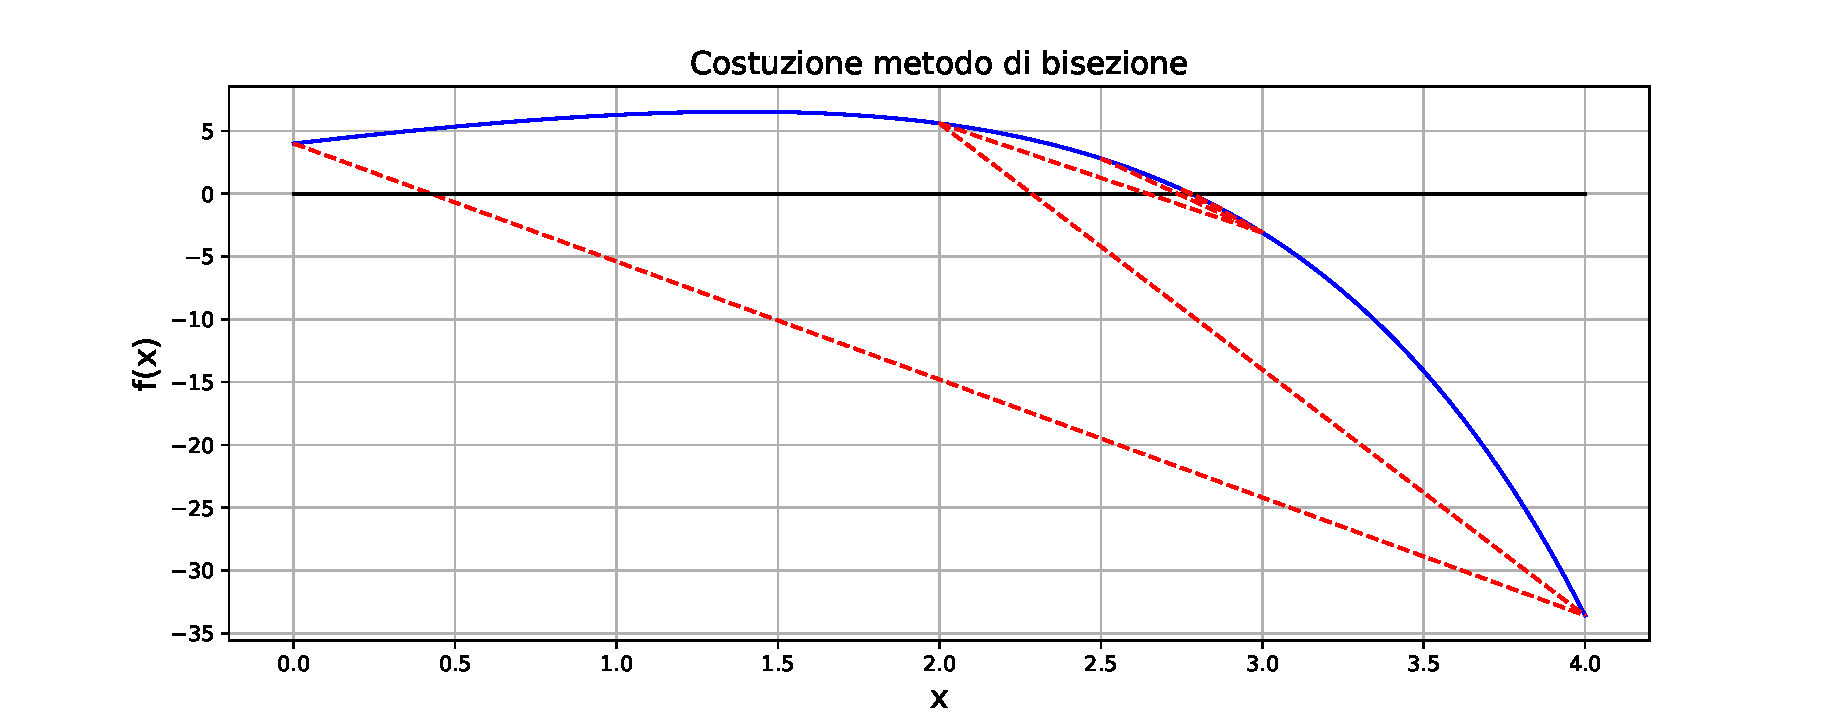
\includegraphics[scale=0.6]{img/co_bis.pdf}
}   
\end{center}

Per generare il grafico precedente si può fare così:

\begin{lstlisting}[language=Python]
import numpy as np
import matplotlib.pyplot as plt

a = 0.0 #estemo sinistro dell'intervallo
b = 4.0 #estremo destro dell'intervallo
t = 1.0e-15 #tolleranza

plt.figure(2)
plt.title('Costuzione metodo di bisezione', fontsize=15)
plt.xlabel('x', fontsize=15)
plt.ylabel('f(x)', fontsize=15)
plt.plot(x, f(x), 'b')
plt.plot([a, b],[f(a), f(b)], linestyle='--', c='r')
plt.plot(x, x*0, 'k')

iter = 1
#fai finche' l'intervallo e' piu' grande della tolleranza
while (b-a) > t:
    c = (a+b)/2.0 #punto medio
    fc = f(c)
    #se hanno lo stesso segno allora c e' piu' vicino allo zero che a
    if fc*fa > 0:
        a = c
    #altrimenti e' b che e' piu' lontano
    else:
        b = c
    iter += 1
    plt.plot([a, b],[f(a), f(b)], linestyle='--', c='r')

plt.grid()
plt.show()
\end{lstlisting}


Il metodo di bisezione non è il migliore in genere per questo tipo di cose però checché se ne dica funziona sempre, quindi in caso non sappiate che pesci pigliare...

\subsection{Metodo di Newton}
Se si considera un $x_0$ molto vicino alla soluzione possiamo espandere in serie di taylor e ottenere:
\[
f(s) = 0 = f(x_0) + (x_0-s)\frac{df}{dx}(x_0) \hspace{5 mm} \text{da cui} \hspace{5 mm} s = x_0 + \frac{f(x_0)}{\frac{df}{dx}(x_0)}
\]
che conduce quini al metodo iterativo:
\[
x_{n+1} = x_n + \frac{f(x_n)}{\frac{df}{dx}(x_n)}
\]
Nel seguente codice utilizzeremo la libreria sympy che permette di eseguire calcoli analitici. Ovviamente qual ora non sia fattibile la derivata va calcolata numericamente.
\begin{lstlisting}[language=Python]
import sympy as sp

x = sp.Symbol('x')
f = sp.tan(x)-x #funzione di cui trovare gli zeri
df = sp.diff(f, x) #derivata della funzione f
t = 1e-13 #tolleranza

def tangenti(x0, t):
    iter = 1
    while abs(f.subs(x, x0))>=t:
        x0 = x0 - ( f.subs(x,x0) / df.subs(x,x0) )
        iter += 1
        if iter > 10000 or abs(f.subs(x, x0))>500:
            if iter > 10000:
                raise Exception('troppe iterazioni')
                
            if abs(f.subs(x, x0))>500:
                raise Exception('la soluzione sta divergendo\nscegliere meglio il punto di partenza')
                
    return x0, iter


#valore iniziale da cui partire
init = 4.4


xs, iter = tangenti(init, t)

print(iter , " iterazioni necessarie")


print("xs= %.15f" %xs)

print("|f(xs)|= %e" %abs(f.subs(x,xs)))

[Output]
7  iterazioni necessarie
xs= 4.493409457909064
|f(xs)|= 8.881784e-16
\end{lstlisting}
 
Per vedere graficamente cosa succede, cambiamo funzione dato che la tangente è troppo ripida e costruiamo come prima il grafico delle iterazioni. Il codice è il seguente:
\begin{lstlisting}[language=Python]
import sympy as sp
from sympy.plotting import plot

x = sp.Symbol('x')
f = x**2 -2 #funzione di cui trovare gli zeri
df = sp.diff(f, x) #derivata della funzione f
t = 1e-13 #tolleranza
init = 4.4
P1 = plot(f, (x, -2, init), ylim=(-2.2, f.subs(x,init)), show=False, title='Costuzione metodo tangenti')

def tangenti(x0, t):
    iter = 1
    while abs(f.subs(x, x0))>=t:
        P2 = plot(f.subs(x,x0)+(x-x0)*df.subs(x,x0), (x, -2, init), ylim=(-2.2, f.subs(x,init)), show=False)
        P1.extend(P2)
        x0 = x0 - ( f.subs(x,x0) / df.subs(x,x0) )
        iter += 1
        if iter > 10000 or abs(f.subs(x, x0))>500:
            if iter > 10000:
                raise Exception('troppe iterazioni')

            if abs(f.subs(x, x0))>500:
                raise Exception('la soluzione sta divergendo\nscegliere meglio il punto di partenza')

    return x0, iter


#valore iniziale da cui partire
xs, iter = tangenti(init, t)

print(iter , " iterazioni necessarie")
print("xs= %.15f" %xs)
print("|f(xs)|= %e" %abs(f.subs(x,xs)))

P1.show()

[Output]
7  iterazioni necessarie
xs= 1.414213562373095
|f(xs)|= 4.440892e-16
\end{lstlisting}

\begin{center}
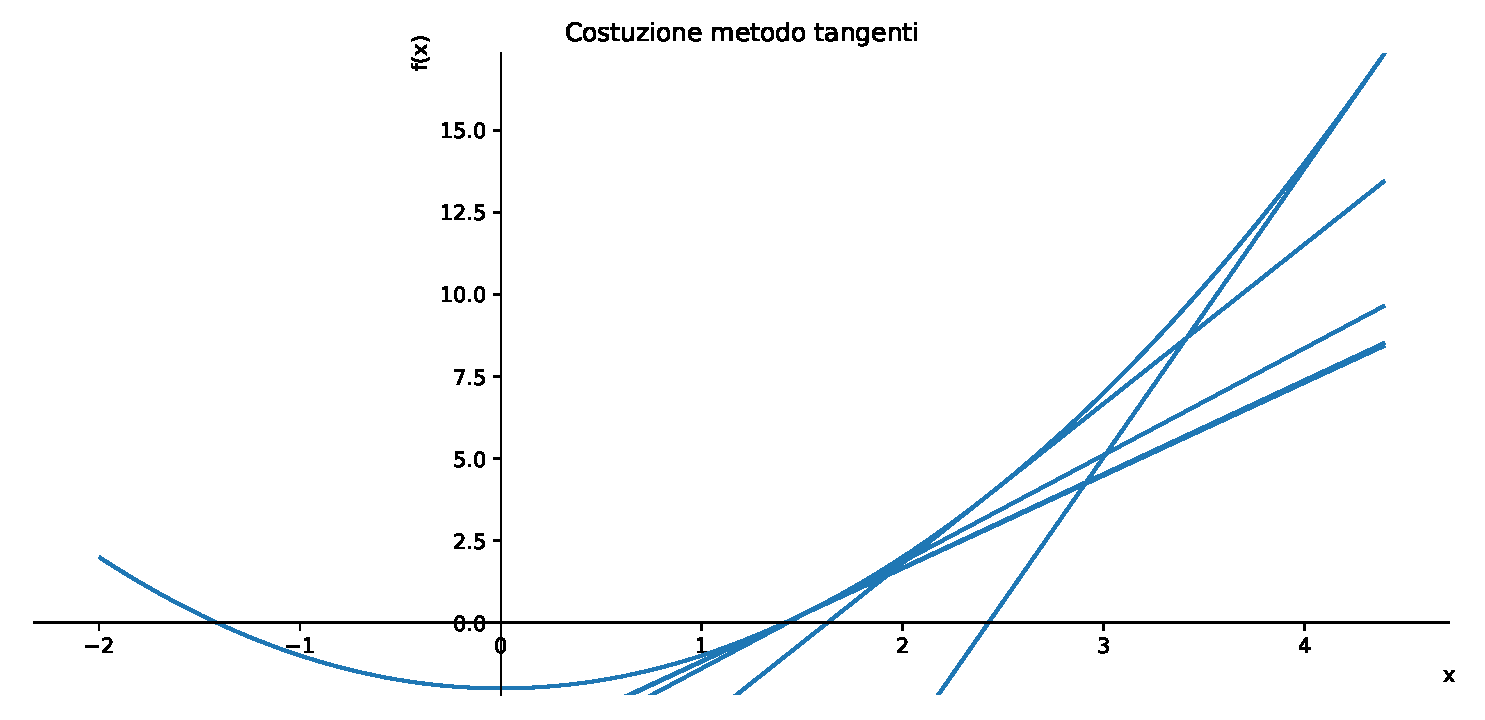
\includegraphics[scale=0.5]{img/co_tan.pdf}  
\end{center}

Purtroppo questo metodo può presentare problemi, provate a risolvere l'equazione $x^3 - 2x + 2 = 0$ vi accorgerete che a seconda di dove partite succedono cose strane...

\subsection{Zeri in più dimensioni}
Ovviamente oltre agli zeri di una singola funzione possiamo anche risolvere un sistema; vedremo sia un 'implementazione manuale, che è il newton raphson, sia un paio di funzioni di scipy. Fondamentalmente newton raphson è come la regola di newton vista sopra, solo che ora x è un vettore e invece della derivata dobbiamo calcolare la matrice delle derivate e invertirla. Passiamo quindi da un sistema non lineare a risolvere diverse volte, per ogni iterazione, un sistema lineare:
\[
\textbf{x}_{n+1} = \textbf{x}_n - J(\textbf{x}_n)^{-1}F(\textbf{x}_n)
\]
Dove $J$ è definito come:
\[
J = \begin{bmatrix} \dfrac{\partial f_1}{\partial x_1} & \cdots & \dfrac{\partial f_1}{\partial x_n} \\ \vdots & \ddots & \vdots \\ \dfrac{\partial f_m}{\partial x_1} & \cdots & \dfrac{\partial f_m}{\partial x_n}  \end{bmatrix} \hspace{10 mm} J_{ij} = \frac{\partial f_i (\mathbf {x})}{\partial x_j}.
\]
Proviamo un caso semplice in cui possiamo anche visualizzare l'evoluzione della soluzione, quindi solo due equazioni:
\[
\begin{cases}
x^2 + y^2 - 1 = 0 \\
y - x^2 + x/2 = 0
\end{cases}
\]
Vediamo il codice con sia implementazione manuale che tramite scipy:

\begin{lstlisting}[language=Python]
"""
newton method for nonlinear system of equations
"""
import numpy as np
import matplotlib.pyplot as plt
from scipy.optimize import fsolve, root

#=============================================================
# Newron method implementation
#=============================================================

def newton(f, start, tol, args=(), dense_output=False, max_it=1000):
    '''
    Generalizzation of newton method for n equations
    
    Parameters
    ----------
    f : callable
        A vector function to find a root of.
    start : ndarray
        Initial guess. The method is very sensitive to this
        must be chosen carefully
    tol :float, optional, default 1e-8
        required tollerance
    args : tuple, optional
        Extra arguments passed to f
    dense_output : bool, optional
        true for full and number of iteration
    max_it : int, optional, default 1000
        after max_it iteration the code stop raising an exception
    
    Return
    ------
    x0 : 1darray
        solution of the system
        if dense_outupt=True all iteration are returned
        in a matrix called X and also the number of iteration
    '''
    
    # initial guess
    x0 = start
    f0 = f(x0, *args)
    # for the computation of jacobian
    nd = len(x0)
    df = np.zeros((nd, nd))
    h  = 1e-8
    s  = np.zeros(nd)
    #for full output
    X = []
    if dense_output : X.append(x0)
    # count
    n_iter = 0
    
    while True:
        
        # compute jacobian using symmetric derivative
        for i in range(nd):       # loop over functions
            for j in range(nd):   # loop over variables
                s[j] = 1
                xr, xl = x0 + h*s, x0 - h*s
                df[i, j] = (f(xr, *args) - f(xl, *args) )[i]/(2*h)
                s[:] = 0
        
        # update solution
        delta = np.linalg.solve(df, f0)
        x0 = x0 - delta
        f0 = f(x0, *args)
        
        if dense_output:
            n_iter += 1        
            X.append(x0)
        
        # stop condition
        if all(abs(f0) < tol):
            break
        # check iterations
        if n_iter > max_it :
            err_msg = 'too many iteration, failure to converge, change initial guess'
            raise Exception(err_msg) 
    
    if dense_output:
        return np.array(X), n_iter       
    else:
        return x0

#=============================================================
# System to solve
#=============================================================        

def system(V):
    x1, x2 = V
    
    r1 = x1**2 + x2**2 - 1#x3
    r2 = x2 - x1**2 + x1/2 #+ x3/5
    #r3 = x3**2 + 5*x2 - 7
    
    R = np.array([r1, r2])#, r3])
    return R

#=============================================================
# Solution and copare with scipy
#=============================================================    

init = np.array([0.2, 0.0])
tol = 1e-12
sol, n_iter = newton(system, init, tol=tol, dense_output=True)
xs, ys = sol.T
print("Solution with newton: ", *sol[-1], "in", n_iter, "iterations")

sol = root(system, init, method='hybr', tol=tol)
print("Solution with root:   ", *sol.x)

sol = fsolve(system , init, xtol=tol)
print("Solution with fsolve: ", *sol)

#=============================================================
# Plot
#=============================================================    

t = np.linspace(0, 2*np.pi, 1000)
z = np.linspace(-0.8, 1.5, 1000)
plt.figure(1)
plt.grid()
plt.plot(np.cos(t), np.sin(t), 'r', label='first equation')
plt.plot(z, z**2- z/2, 'b', label='second equation')
plt.plot(xs, ys, 'k', label='evolution of solution')
plt.legend(loc='best')
plt.show()

[Output]
Solution with newton:  0.9214908788160613 0.38840000033316596 in 7 iterations
Solution with root:    0.9214908788160611 0.388400000333166
Solution with fsolve:  0.9214908788160611 0.388400000333166

\end{lstlisting}
Vediamo che il nostro codice funziona ci sono però un paio di problemi. Esso presenta problemi simili a quello unidimensionale. Ci sono casi in cui lo jacobiano può non esistere, o essere singolare. Inoltre se già gli algoritmi sofisticati sono sensibili alle condizioni iniziali, questo metodo, essendo molto base, lo è infinitamente di più. Provate a cambiare un po' il valore della guess iniziale e vedrete il macello che si combina. Una strategia spesso usata, che è ciò che fa scipy (non a caso le funzioni se avete notato sono nella libreria "scipy.optimize", la stessa di "curve\_fit"), è quella di promuovere il problema dalla ricerca di uno zero alla ricerca di un minimo. Ovvero si passa da cercare lo zero di $f_i$ alla ricerca del minimo della somma su i delle $f_i$ al quadrato $S^2 = \sum_i f_i^2$. Con qualche modifica si può anche usare metodo visto per fare i fit ma la cosa migliore e in genere più usata è risolvere questi problemi con degli algoritmi chiamati "trust-region".

\begin{center}
    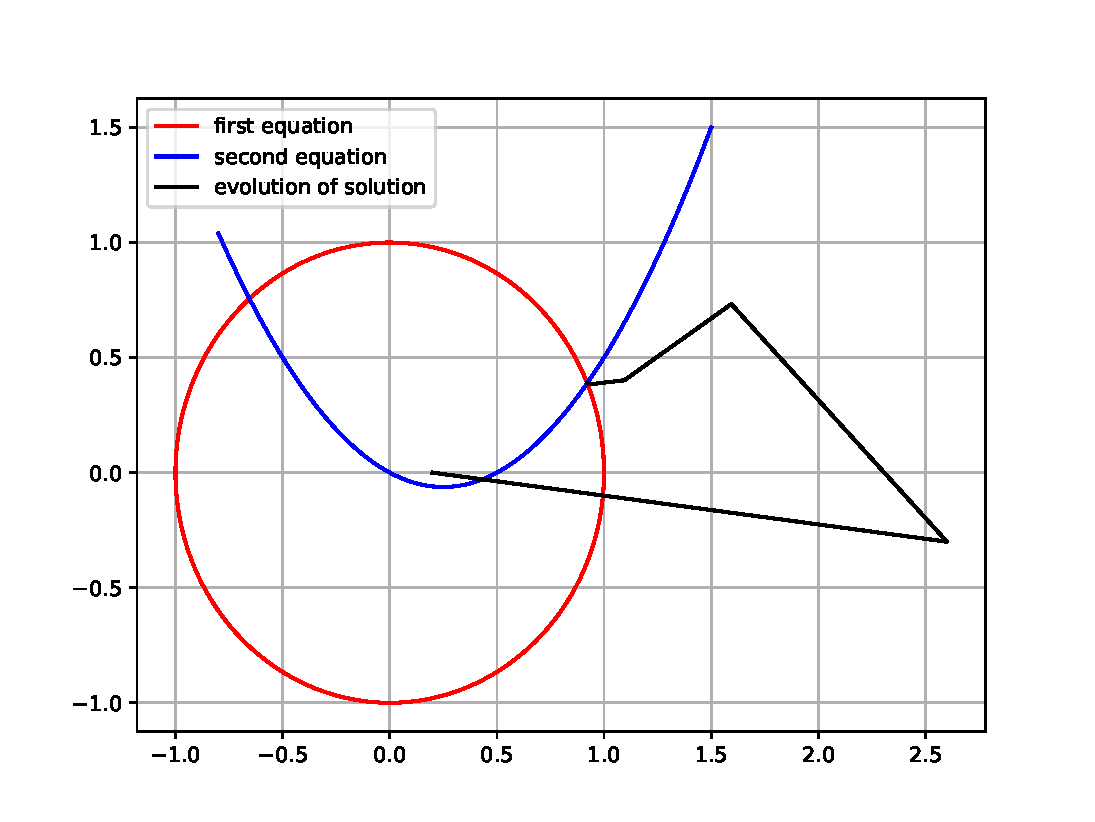
\includegraphics[scale=0.85]{img/NR.pdf}
\end{center}

\newpage

\section{Calcolo degli integrali}
Avere a che fare con integrali di cui non si conosce l'espressione analitica è una cosa estremamente comune in fisica, anche troppo. Bisogna quindi trovare un modo per poter calcolare i vari integrali. Molti sono i metodi usati, qui voglia illustrare un metodo di quadratura gaussiana, il metodo di Gauss-Legendre. Questo metodo ci permette di approssimare l'integrale con una somma pesata:
\begin{equation}
\int_{-1}^{1} f(x) \simeq \sum_{i=1}^n w_i f(x_i) \quad,
\end{equation}
dove $n$ è il numero di punti, $x_i$ sono le radici del polinomio di Legendre di grado n $P_n(x)$, e $w_i$ sono definiti come:
\begin{equation}
w_i = \frac{2}{(1-x_i^2)(P_n^{'}(x_i))^2}\quad.
\end{equation}
Questo però ci da solo integrali nell'intervallo $[-1, 1]$, problema facilmente risolvibile considerando un cambio di variabili:
\begin{equation} \label{inte}
I_{ab} = \int_a^b f(x) \simeq \frac{b-a}{2} \sum_{i=1}^n w_i f \Biggl(x_i \frac{b-a}{2} + \frac{b + a}{2} \Biggr) \quad.
\end{equation}
Ora in linea di principio basterebbe questo, calcoliamo quella somma una volta ed abbiamo finito. Però vogliamo fare qualcosa di più, vogliamo fare un algoritmo adattivo. Quello che facciamo è: scelti $a$ e $b$ estremi in integrazione calcoliamo l'integrale poi detto $m=(a+b)/2$ il punto medio calcoliamo l'integrale nei due sotto intervalli; se la differenza fra l'integrale intero e la somma degli integrali sui due sotto intervalli è piccola, abbiamo finito, altrimenti ripartiamo ricorsivamente dividendo ciascun intervallo in altri due intervalli et cetera. Possiamo così attribuire facilmente un errore al nostro integrale, useremo proprio la differenza che usiamo come criterio di convergenza. Vediamo dal punto di vista del codice:

\begin{lstlisting}[language=Python]
"""
code for integration with Gauss-Legendre quadrature
"""

import math
from scipy.special import roots_legendre

def adaptive_gaussleg_quadrature(f, a, b, args=(), tol=1e-8, n=5):
    """
    Splits an integral into the right and left half
    and compares it to the integral on the whole interval
    if tolerance is not satisfied, left and right are
    splitted into smaller intervals and so on until the
    tolerance is satisfied they are added to the sum

    Parameters
    ----------
    f : callable
        function to integrate
    a : float
        beginning of the interval
    b : float
        end of the interval
    args : tuple, optional
        extra arguments to pass to f
    tol : float, optional
        tollerance, default 1e-8
    n : int, optional
        number of nodes, default n=5

    Return
    ----------
    Int : float
        \int_a^b f
    diff : float
        error on Int
    """

    #interval divison
    m = a + (b - a)/2
    #compute integral
    Int = gauss_leg(f, a, b, args, n)
    I_r = gauss_leg(f, m, b, args, n)
    I_l = gauss_leg(f, a, m, args, n)
    #check tollerance
    diff = abs( Int - (I_l + I_r) )
    if diff < tol:
        return Int, diff
    #recursive call
    div1, err1 = adaptive_gaussleg_quadrature(f, m, b, args, tol, n)
    div2, err2 = adaptive_gaussleg_quadrature(f, a, m, args, tol, n)
    #sum of all integrals in the several intervals
    x = div1 + div2
    r = err1 + err2

    return x, r


def gauss_leg(f, a, b, args=(), n=5):
    """
    Calculation of the integral of f
    with the Gaussian-Legendre quadrature method

    Parameters
    ----------
    f : callable
        function to integrate
    a : float
        beginning of the interval
    b : float
        end of the interval
    args : tuple, optional
        extra arguments to pass to f
    n : int
        number of nodes, default n=5

    Return
    ----------
    Inte : float
        \int_a^b f
    """

    #b must be grather tha a
    if b < a:
        a, b = b, a
    else : pass

    Inte = 0
    dxdxi = (b - a)/2
    roots, weights = roots_legendre(n)

    for x_i, w_i in zip(roots, weights):
        Inte += w_i * f(x_i * dxdxi + (b + a)/2, *args)

    Inte *= dxdxi

    return Inte


def test():
    """ little test
    """
    def h(x):
        """sine
        """
        return math.sin(x)
    def f(x, a1):
        """gaussian
        """
        return math.exp(-x**2/(2*a1))/(math.sqrt(2*math.pi)*a1)
    def g(x, a1, a2):
        """fermi dirac
        """
        return math.exp(-(x - a1)/a2)/(1 + math.exp(-(x - a1)/a2))

    I, dI = adaptive_gaussleg_quadrature(h, 0, math.pi)
    print('Integral value is', I, '+-', dI)
    I, dI = adaptive_gaussleg_quadrature(f, -100, 100, args=(1,))
    print('Integral value is', I, '+-', dI)
    I, dI = adaptive_gaussleg_quadrature(g, 0, 20, args=(10, 0.02))
    print('Integral value is', I, '+-', dI)


if __name__ == '__main__':

    test()

[Output]
Integral value is 2.0000000000791305 +- 7.905831544974262e-11
Integral value is 1.0000000051542988 +- 5.442503145328187e-09
Integral value is 10.0 +- 0.0
\end{lstlisting}

Volendo fare un confronto con una funzione Python quella adatta è "sicpy.integrate.quad" la quale adopera sempre una quadratura gaussiana ma con pesi e nodi diversi, infatti usa la tecnica: 21-point Gauss–Kronrod quadrature, con una leggera modifica. Non se ne riporta l'implementazione in quanto sarebbe analogo tolta la parte dei nodi che però son tabulati (più di 400 linee di codice). Nella cartella sarà tuttavia presente per chi fosse interessato. Giusto per completezza facciamo notare che in Gauss–Kronrod l'errore è calcolato in maniera diversa e più efficiente. Si considerano infatti due integrali che denominiamo GN, KM, rispettivamente per Gauss e Kronrod, uno calcolato in N punti e l'altro in M e come errore si considera la differenza del valore assoluto. L'implementazione di scipy è basata su (G$10$, K$21$). Nella cartella è presente il codice in cui sono raccolte le seguenti possibili composizioni ('gkdata.py'): (G$7$,  K$15$), (G$10$, K$21$), (G$15$, K$31$), (G$20$, K$41$), (G$25$, K$51$), (G$30$, K$61$).

\newpage

\section{Risolvere numericamente le ODE: IVP}
In questa sezione ci occuperemo dei così-detti problemi ai valori iniziali (initial value problem IVP).\\
In fisica è prassi che spuntino fuori equazioni differenziali che non ammettano soluzione analitica; piuttosto che lamentarci di questo ringraziamo quando ciò capita con le ODE, cioè le equazione differenziali ordinarie, perché spesso e volentieri madre natura preferisce l'utilizzo delle equazioni differenziali alle derivate parziali(dette PDE) che in genere da risolvere sono abbastanza più complicate. Qui vedremo semplici esempi per risolvere un'ode.
I metodi mostrati saranno per brevità solo due: l'utilizzo delle funzione "odeint()" di scipy e il metodo di eulero, basato sulla definizione di derivata, che mostriamo brevemente:
sia 
\begin{equation}
\begin{cases}
f^{'}(t)=g(t, f(t))	 \hspace{10 mm} \text{equazione differenziale}\\
x(t_0) = x_0 \hspace{19.5 mm} \text{condizione iniziale}
\end{cases}
\end{equation}
il problema ai valori iniziali da risolvere ,allora:
\begin{equation}
f^{'}=\frac{df}{dt} \xrightarrow{discretizzando} \frac{f(t+dt)-f(t)}{dt}
\end{equation}
Dove la forma ottenuta discretizzando non è altro che il rapporto incrementale di $f(t)$, di cui per definizione la derivata ne è il limite per $dt \to 0$.  Sapendo la forma funzionale della derivata, ovvero la $g(t, f(t))$, data dall'equazione differenziale, possiamo ottenere la soluzione dell'equazione per passi:
\begin{equation}
f(t+dt) = f(t) + dt \, g(t, f(t))
\end{equation}
quindi possiamo trovare la soluzione al tempo t+dt, sapendo quella al tempo t, e andando a ritroso, grazie alla condizione iniziale possiamo avere tutta la soluzione. Inoltre nella g non compare la dipendenza da $f(t+dt)$ ma solo da $f(t)$, per questo il metodo è chiamato esplicito. Importante notare che la discretizzazione che abbiamo deciso di usare è del tutto arbitraria (la più semplice possibile che ci da appunto il metodo di Eulero), e anche il passo $dt$ è un argomento delicato, vediamo perché.

\subsection{Calcolo delle derivate}
Vediamo un esempio di come varia l'errore nel calcolo di una derivata numerica al variare dell'incremento:

\begin{lstlisting}[language=Python]
import numpy as np
import matplotlib.pyplot as plt

def f(x):
    '''
    funzione di cui calcolare la derivata
    '''
    return np.exp(x)

def df(f, x, h):
    """
    derivata di f
    """
    dy = (f(x+h) - f(x))/h
    return dy

#array del passo di discretizzazione
h = np.logspace(-15, -1, 1000)

plt.figure(1)
plt.title('errore derivata al variare del passo', fontsize=15)
plt.ylabel('erorre derivata', fontsize=15)
plt.xlabel("grandezza dell'incremento", fontsize=15)

plt.plot(h, abs(df(f, 0, h)-f(0)))

plt.xscale('log')
plt.yscale('log')
plt.grid()
plt.show()

\end{lstlisting}

\begin{center}
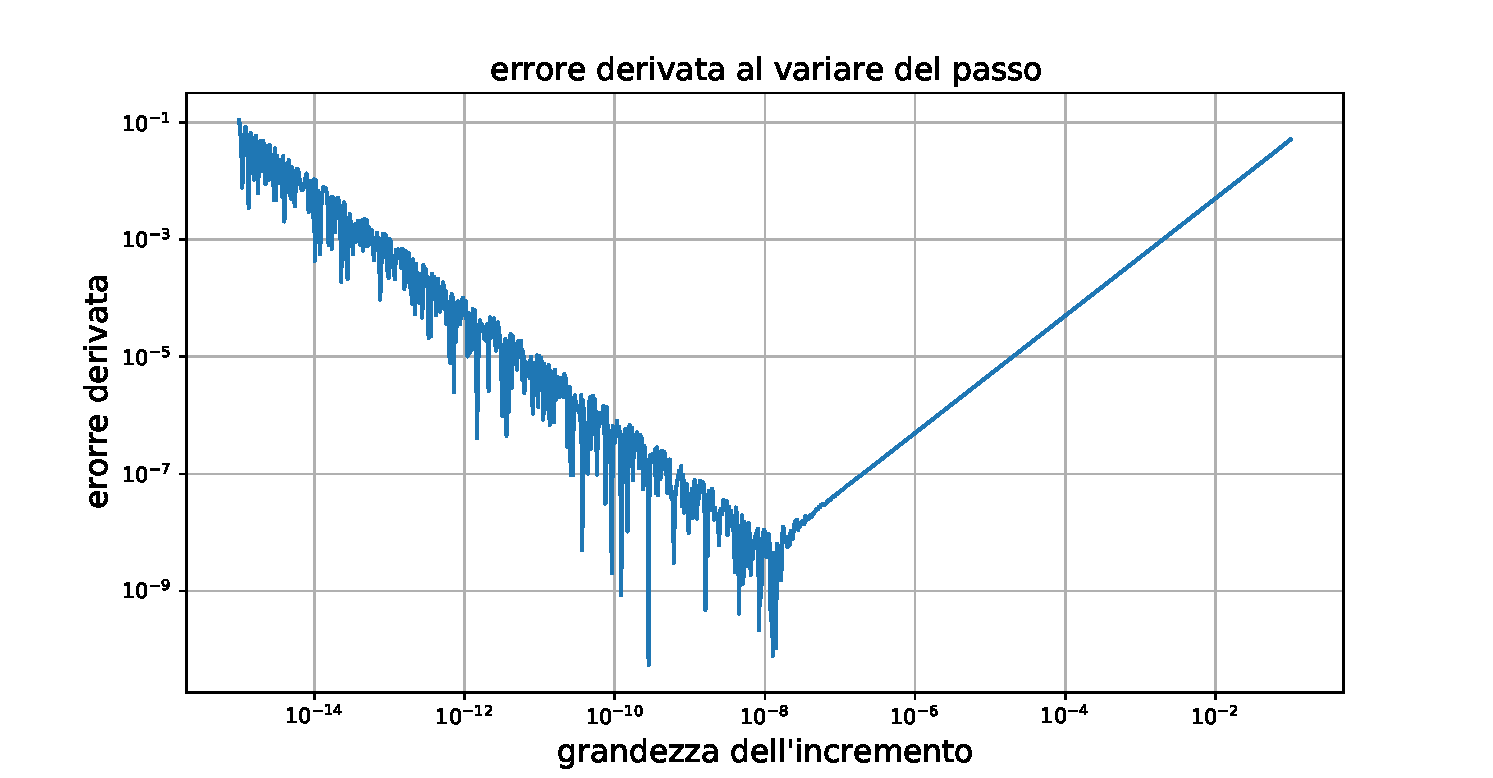
\includegraphics[scale=0.7]{img/err_deriv.pdf}

\end{center}

vediamo quindi come un passo di $10^{-14}$ che intuitivamente potremmo credere migliore da lo stesso errore di un passo di $10^{-2}$. Inoltre tutta la trattazione è immancabilmente affetta dal metodo di approssimazione che usiamo. Un algoritmo di alto ordine darà risultati migliori con un passo grande piuttosto che uno piccolo. Vediamo diversi modi di approssimare una derivata prima:
\begin{align}
f^{'} &= \frac{f(x+h) - f(x)}{h} \\
f^{'} &= \frac{f(x) - f(x-h)}{h} \\
f^{'} &= \frac{f(x+h) - f(x-h)}{2h} \\
f^{'} &= \frac{-3f(x) + 4f(x+h) - f(x+2h) }{2h} \\
f^{'} &= \frac{ 3f(x) - 4f(x-h) + f(x-2h) }{2h} \\
f^{'} &= \frac{-f(x+2h) + 8f(x+h) - 8f(x-h) + f(x-2h)}{12h}
\end{align}
Rispettivamente i primi due due primo ordine, i seguenti tre del secondo ordine e il terzo del quarto ordine. Vediamo un piccolo codice nel quale vi potete divertire a cambiare la grandezza passo per rendervi conto di quanto dicevamo:
\begin{lstlisting}[language=Python]
"""
Code that compiles some method of calculating a derivative to various orders of accuracy
"""
import numpy as np
import matplotlib.pyplot as plt


def d1b(f, x0, dx):
    '''first order, backward derivative
    '''
    dfdx = (f(x0) - f(x0-dx))/dx
    return dfdx

def d1f(f, x0, dx):
    '''first order, forward derivative
    '''
    dfdx = (f(x0+dx) - f(x0))/dx
    return dfdx

def d2c(f, x0, dx):
    '''second order, symmetric derivative
    '''
    dfdx = (f(x0+dx) - f(x0-dx))/(2.0*dx)
    return dfdx

def d2f(f, x0, dx):
    ''' second order forward derivative
    '''
    dfdx = ( - 3.0*f(x0) + 4.0*f(x0+dx) - f(x0+2.0*dx) )/(2.0*dx)
    return dfdx

def d2b(f, x0, dx):
    ''' second order backward derivative
    '''
    dfdx = ( 3.0*f(x0) - 4.0*f(x0-dx) + f(x0-2.0*dx) )/(2.0*dx)
    return dfdx

def d4c(f, x0, dx):
    ''' fourth order centered derivative
    '''
    dfdx = ( -f(x0+2*dx) + 8.0*f(x0+dx) - 8.0*f(x0-dx) + f(x0-2*dx) )/(12.0*dx)
    return dfdx

#==================================================================
# Plot
#==================================================================

plt.figure(1, figsize=(12, 8))
x = np.linspace(0, 2*np.pi, 100)
f = np.sin
g = np.cos
h = 1e-4
Df = [d1b, d1f, d2c, d2f, d2b, d4c]
l  = ['first order backward', 'first order forward', 'symmetric', 
      'second order forward', 'second order backward', 'fourth order central']

for i, df in enumerate(Df):
    plt.subplot(2, 3, i+1)
    plt.title(l[i])
    plt.plot(x, g(x)-np.array([df(f, t, h) for t in x]), 'blue')
    plt.grid()

plt.tight_layout()
plt.show()
\end{lstlisting}

\begin{center}
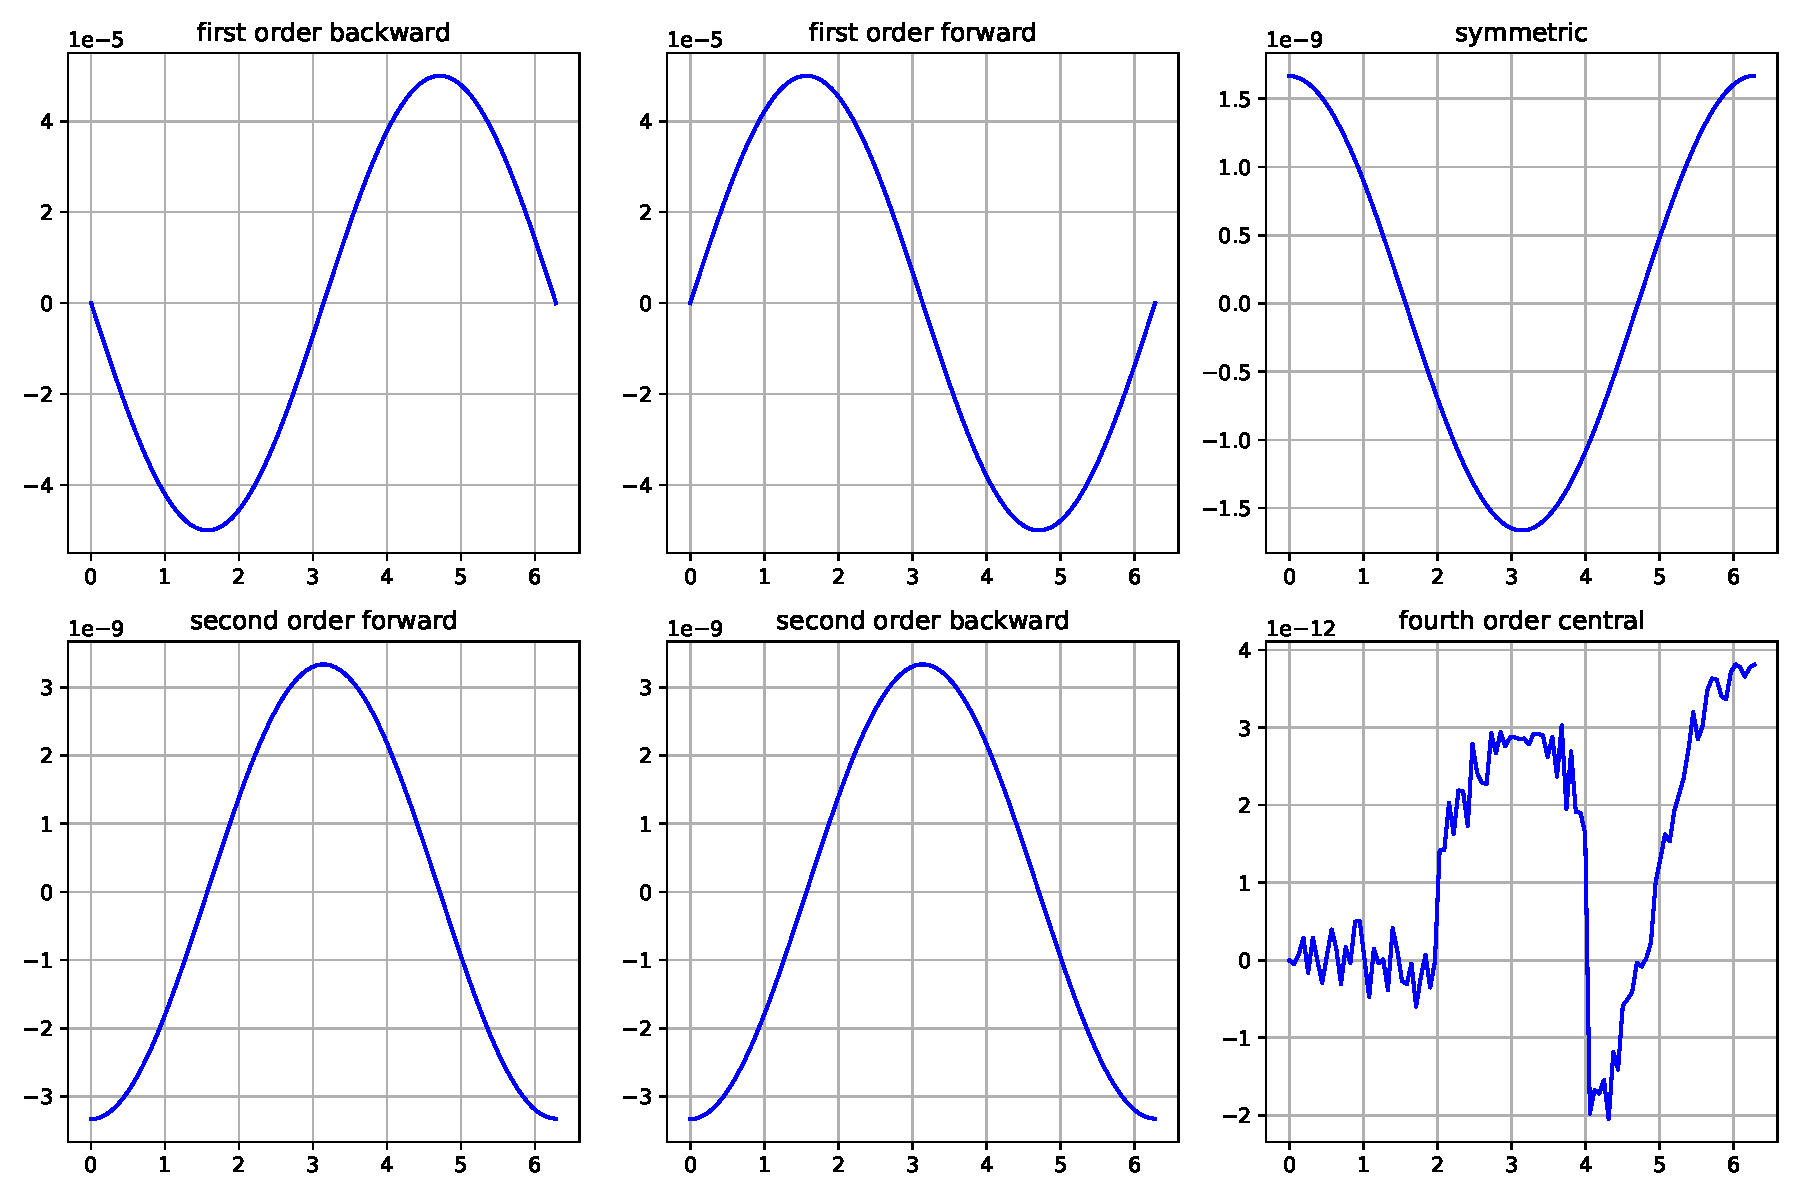
\includegraphics[scale=0.5]{img/cfr_deriv.pdf}
\end{center}
Se aggiungiamo al codice precedente queste poche righe possiamo effettuare lo stesso plot fatto inizialmente:
\begin{lstlisting}[language=Python]
#array del passo di discretizzazione
h = np.logspace(-15, -1, 1000)
s = ['-', '-', '--', '--', '--', '-.']
c = ['r', 'b', 'k', 'r', 'b', 'k']
plt.figure(2)
plt.title('Errore derivata al variare del passo', fontsize=15)
plt.ylabel('erorre derivata', fontsize=15)
plt.xlabel("grandezza dell'incremento", fontsize=15)

for i, df in enumerate(Df):
    plt.plot(h, abs(df(f, 0.5, h)-g(0.5)), label=l[i], linestyle=s[i], color=c[i])

plt.xscale('log')
plt.yscale('log')
plt.legend(loc='best')
plt.grid()
plt.show()
\end{lstlisting}
\begin{center}
\makebox[\textwidth][c]{
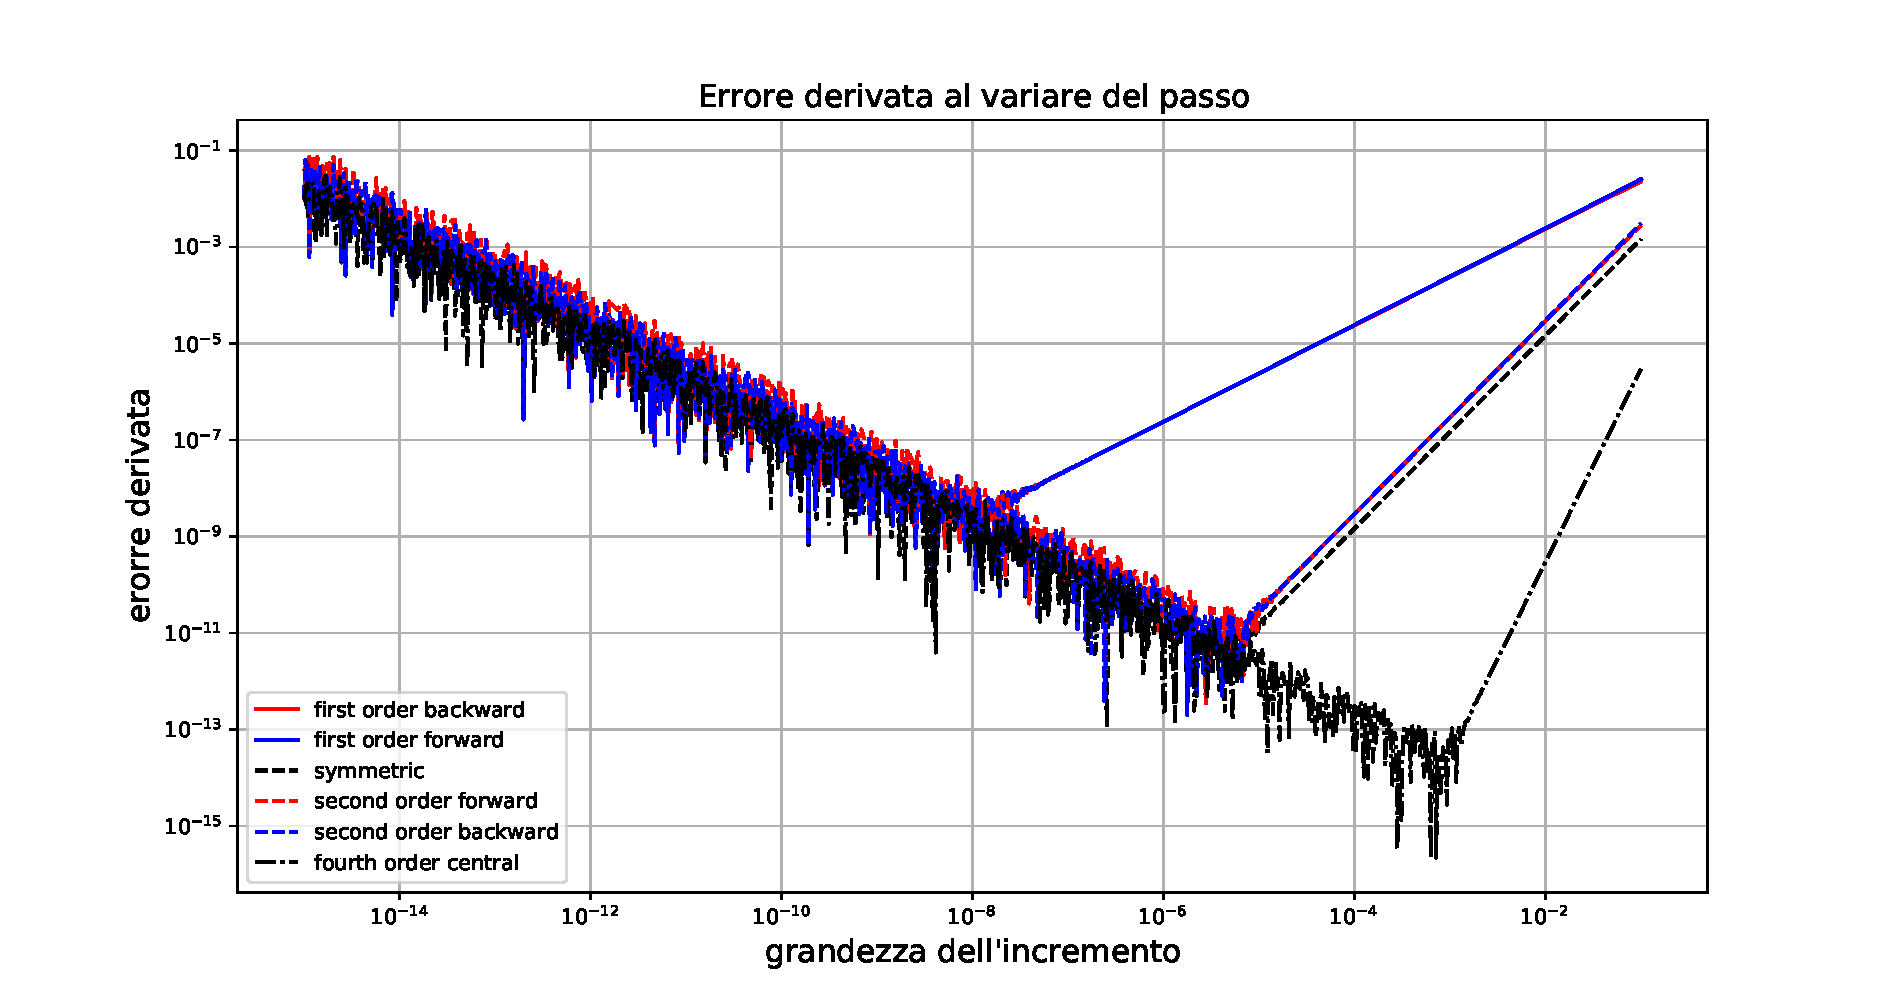
\includegraphics[scale=0.6]{img/cfr_deriv_2.pdf}
}
\end{center}
Potete divertirvi a prendere le parti finali delle curve e calcolare i coefficienti angolari, se c'è giustizia a questo mondo, essi saranno parenti di 1, 2 e 4.


\subsection{Esponenziale}
Passiamo ora alle equazioni differenziali vere e proprie. Cominciamo con il problema di Cauchy:
\[
\begin{cases}
\frac{d x(t)}{dt} = x(t)	\\
x(t=0) = 1
\end{cases}
\]
Abbiamo una funzione incognita x(t) di cui sapiamo che la derivata è uguale a se stessa e che calcolata in zero restituisce uno. Nella fattispecie la soluzione è semplice, si stratta di un esponenziale crescente, tuttavia vediamo come risolvere numericamente tale equazione.

\begin{lstlisting}[language=Python]
import numpy as np
import scipy.integrate
import  matplotlib.pyplot as plt

#parametri
x0 = 1     #condizione inizale
tf = 2     #fino a dove integrare
N = 10000  #numero di punti

#odeint
def ODE_1(y, t):
    """
    equzione da risolvere per odeint
    """
    x = y
    dydt = x
    return dydt
    
 
y0 = [x0] #x(0)
t = np.linspace(0, tf, N+1)
sol = scipy.integrate.odeint(ODE_1, y0, t)

x_scipy = sol[:,0]

#metodo di eulero
def ODE_2(x):
    """
    equzione da risolvere per eulero
    """
    x_dot = x
    return x_dot
    
def eulero(N, tf, x0):
    """
    si usa che dx/dt = (x[i+1]-x[i])/dt 
    che e' praticamente la definizione di rapporto incrementale
    discretizzata la derivata sappiamo a cosa eguagliarla
    perche dx/dt = g(x(t)) nella fattispecie g(x) = x
    quindi discretizzando tutto:
    (x[i+1]-x[i])/dt = x[i]
    da cui si isola x[i+1]
    """
    dt = tf/N #passo di integrazione
    x = np.zeros(N+1)
    x[0] = x0
    
    for i in range(N):
        x[i+1] = x[i] + dt*ODE_2(x[i])
        
    return x

x_eulero = eulero(N, tf, x0)

plt.figure(1)

ax1 = plt.subplot(211)
ax1.set_title('Risoluzione numerica', fontsize=15)
ax1.set_xlabel('t', fontsize=15)
ax1.set_ylabel('x', fontsize=15)
ax1.plot(t, x_scipy, label='scipy')
ax1.plot(t, x_eulero, label='elulero')
ax1.legend(loc='best')
ax1.grid()

ax2 = plt.subplot(223)
ax2.set_title('Differenza tra metodo di eulero e soluzione esatta', fontsize=15)
ax2.set_xlabel('t', fontsize=15)
ax2.set_ylabel('errore', fontsize=15)
ax2.plot(t, x_eulero-np.exp(t))
ax2.grid()


ax3 = plt.subplot(224)
ax3.set_title('Differenza tra odeint e soluzione esatta', fontsize=15)
ax3.set_xlabel('t', fontsize=15)
ax3.set_ylabel('errore', fontsize=15)
ax3.plot(t, x_scipy-np.exp(t))
ax3.grid()

plt.show()
\end{lstlisting}

\begin{center}
\makebox[\textwidth][c]{
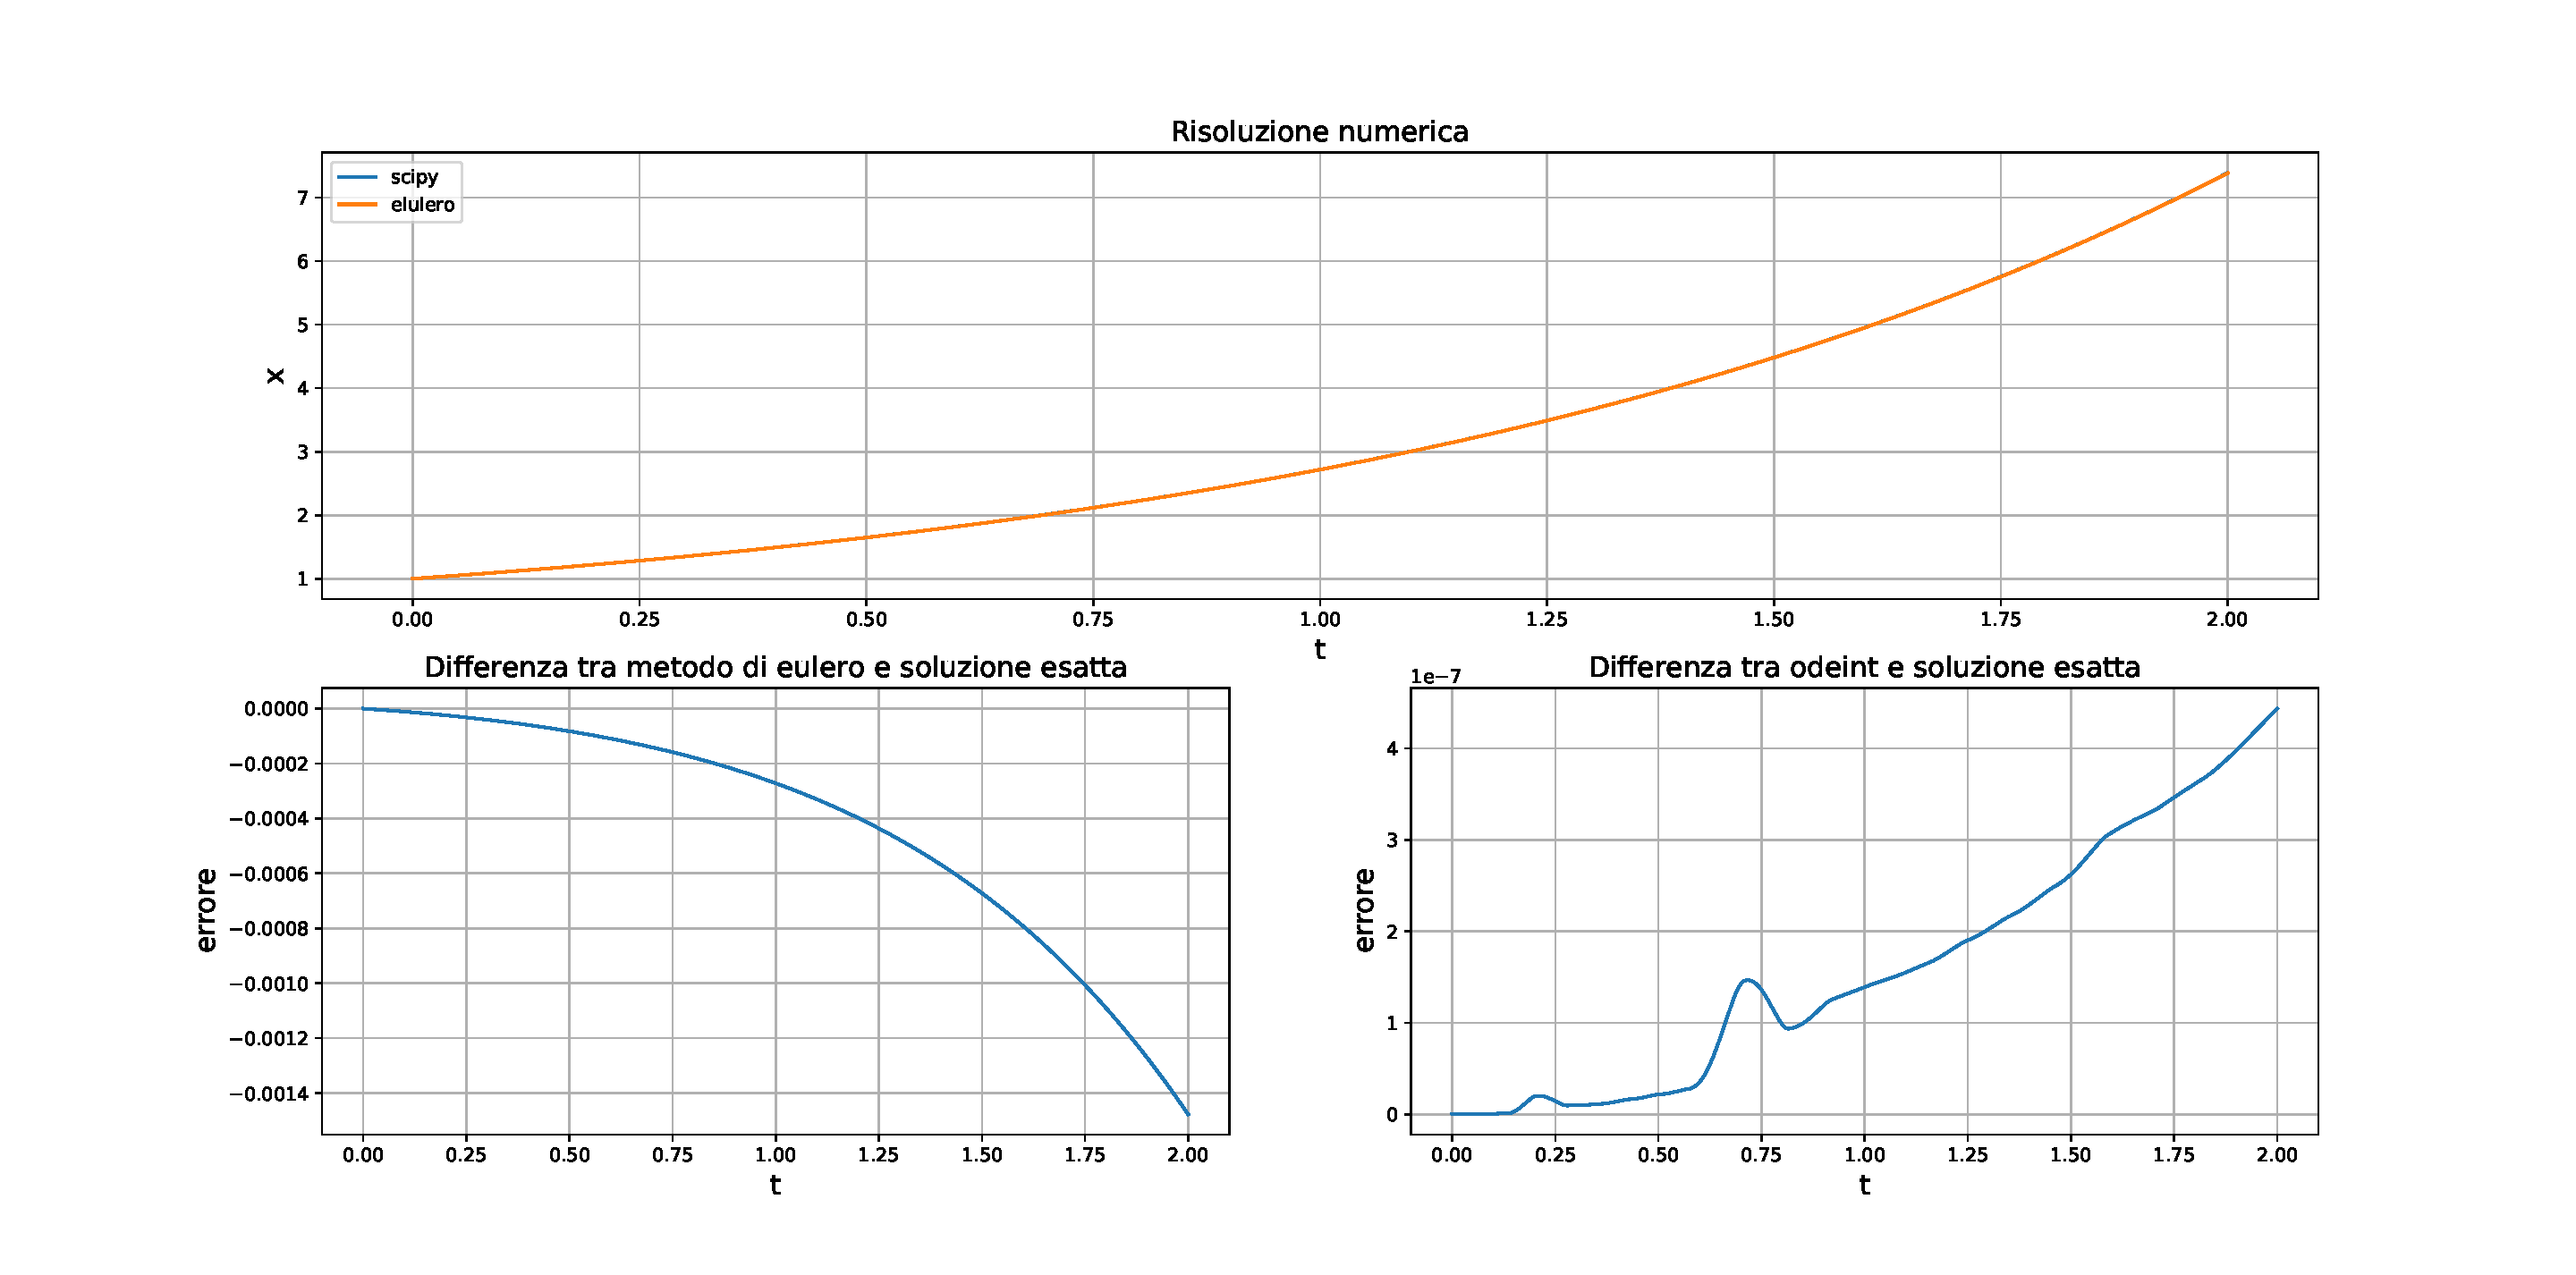
\includegraphics[scale=0.4]{img/ode_1.pdf}
}
\end{center}

Vediamo che entrambi i metodi sembrano funzionare bene, scipy usa un integratore migliore rispetto ad eulero infatti vediamo che la differenza fra le due soluzioni e dell'ordine di $10^{-7}$, ma costruirne uno analogo non è difficile, si può provare con i metodi di Runge-kutta; famoso e molto usato è quello di ordine 4.
Abbiamo risolto un'ode del primo ordine, e per ordine più elevati la cosa è analoga perché con cambi di variabili si può abbassare l'ordine fino ad ottenere un sistema di ode accoppiate di ordine 1;

\subsection{Pendolo}
Vediamo un esempio sta volta con un'equazione che non sappiamo risolvere:

\[
\begin{cases}
\frac{d^2 x(t)}{dt^2} = -\frac{l}{g}sin(x(t))	\\
\frac{d x(t)}{dt}|_{t=0} = v_0 \\
x(t=0) = x_0
\end{cases}
\hspace{10 mm}
\Rightarrow
\hspace{10 mm}
\begin{cases}
\frac{d x(t)}{dt} = v(t)	\\
\frac{d v(t)}{dt} = -\frac{l}{g}sin(x(t)) \\
x(t=0) = x_0 \\
v(t=0) = v_0
\end{cases}
\]
È la famosa equazione del pendolo semplice che approssimata dà luogo all'oscillatore armonico ovvero a tutta la fisica. Vediamo come si modifica il codice di sopra ora:

\begin{lstlisting}[language=Python]
import numpy as np
import scipy.integrate
import  matplotlib.pyplot as plt

#parametri
N = 100000      #numero di punti
l = 1           #lunghezza pendolo
g = 9.81        #accellerazione di gravita'
o0 = g/l        #frequenza piccole oscillazioni
v0 = 0          #condizioni iniziali velocita'
x0 = np.pi/1.1	#condizioni iniziali posizione
tf = 15         #fin dove integrare

#odeint
def ODE_1(y, t):
    """
    equzione da risolvere per odeint
    """
    theta, omega = y
    dydt = [omega,  - o0*np.sin(theta)]
    return dydt
    
 
y0 = [x0, v0] #x(0), x'(0)
t = np.linspace(0, tf, N+1)
sol = scipy.integrate.odeint(ODE_1, y0, t)

x_scipy = sol[:,0]

#metodo di eulero
def ODE_2(x, v):
    """
    equzione da risolvere per eulero
    """
    x_dot = v
    v_dot = -o0*np.sin(x)
    return x_dot, v_dot
    
def eulero(N, tf, x0, v0):
    """
    si usa che dx/dt = (x[i+1]-x[i])/dt 
    che e' praticamente la definizione di rapporto incrementale
    discretizzata la derivata sappiamo a cosa eguagliarla
    perche dx/dt = g(x(t)) nella fattispecie g(x) = x
    quindi discretizzando tutto:
    (x[i+1]-x[i])/dt = x[i]
    da cui si isola x[i+1]
    """
    dt = tf/N #passo di integrazione
    x = np.zeros(N+1)
    v = np.zeros(N+1)
    x[0], v[0] = x0, v0
    
    for i in range(N):
        dx, dv = ODE_2(x[i], v[i])
        x[i+1] = x[i] + dt*dx
        v[i+1] = v[i] + dt*dv
        
    return x, v

x_eulero, _ = eulero(N, tf, x0, v0)


plt.figure(1)

plt.title('Pendolo semplice')
plt.xlabel('t')
plt.ylabel('x')
plt.plot(t, x_scipy, label='scipy')
plt.plot(t, x_eulero, label='elulero')
plt.legend(loc='best')
plt.grid()

plt.show()
\end{lstlisting}

\begin{center}
\makebox[\textwidth][c]{
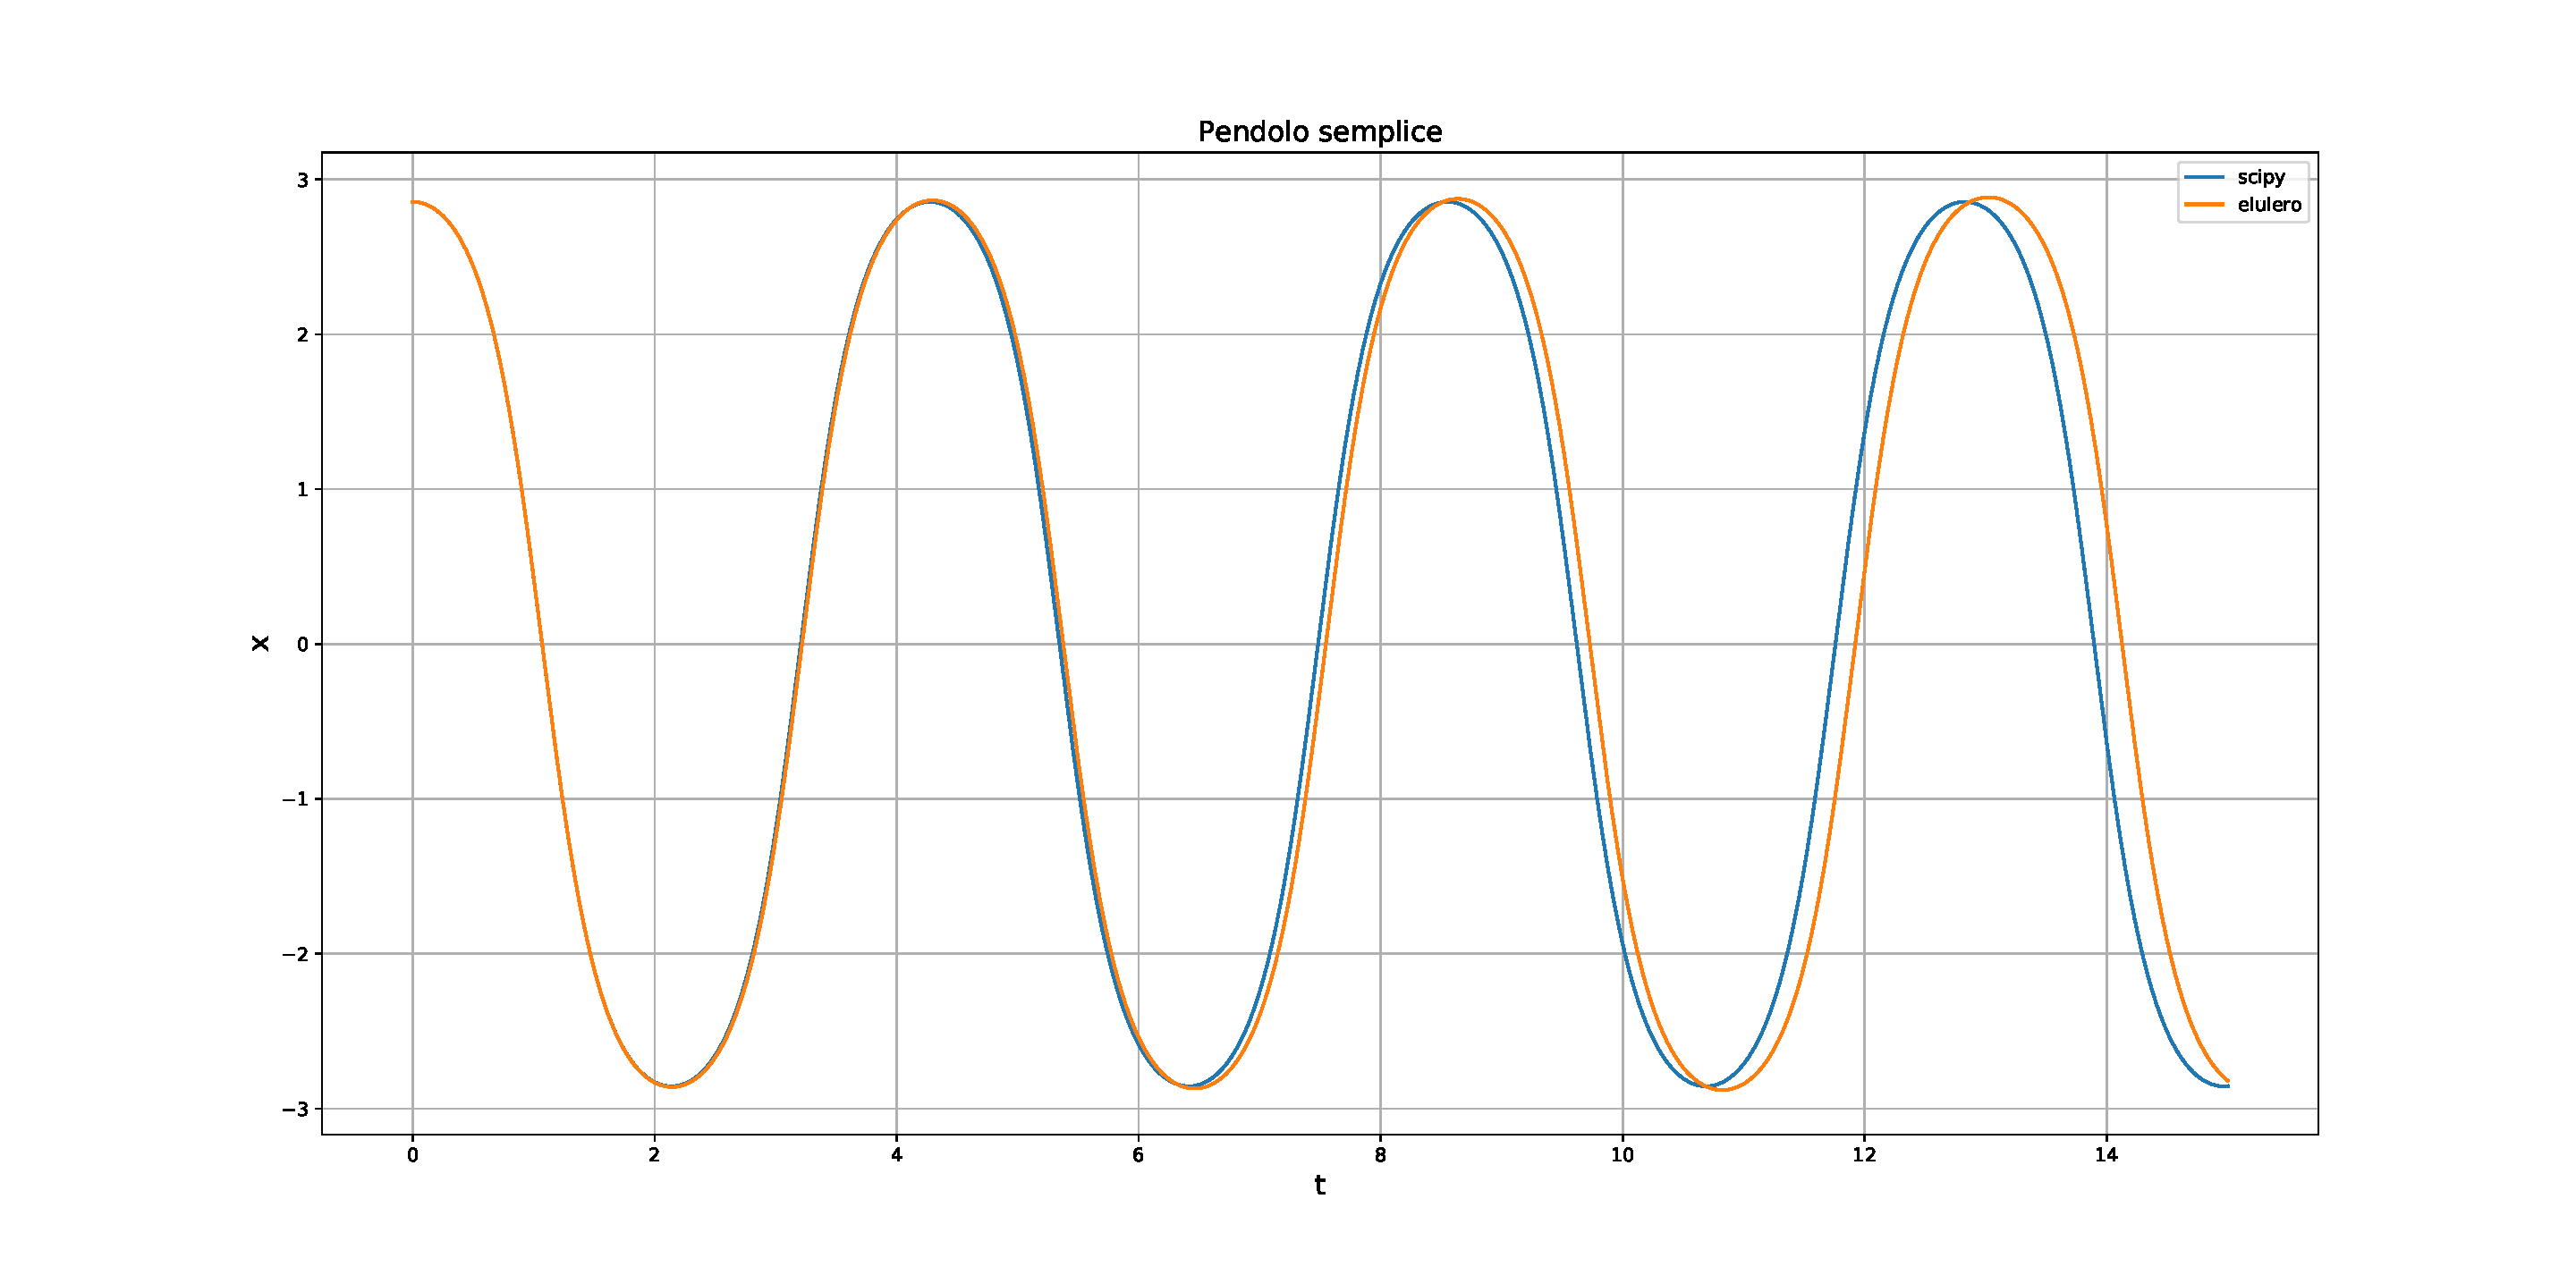
\includegraphics[scale=0.36]{img/ode_2.pdf} 
}
\end{center}


Dal grafico vediamo le due soluzione distaccarsi, questo è dovuto al fatto che l'integrazione con il metodo di eulero non è delle migliori perché è un metodo del primo ordine e il passo di integrazione non è sufficientemente piccolo; si potrebbe fare tutta una trattazione su come scegliere il passo di integrazione anche più approfondita di quanto abbiamo trattato prima, inoltre menzioniamo  che esistono poi algoritmi adattivi in cui il valore del passo può cambiare durante l'integrazione.

\subsection{Animazione}
Abbiamo simulato il movimento del pendolo semplice e abbiamo visto il grafico dell'ampiezza in funzione del tempo ma sarebbe carino riprodurre il movimento del pendolo e creare un'animazione semplice ma comunque realistica. Grazie a matplotlib possiamo farlo senza troppi problemi. Per quanto visto sopra useremo come integratore la funzione "odeint()".




\begin{lstlisting}[language=Python]
import numpy as np
import scipy.integrate
from matplotlib import animation
import  matplotlib.pyplot as plt

#parametri
N = 10000       #numero di punti
l = 1           #lunghezza pendolo
g = 9.81        #accellerazione di gravita'
o0 = g/l        #frequenza piccole oscillazioni
v0 = 0          #condizioni iniziali velocita'
x0 = np.pi/1.1	#condizioni iniziali posizione
tf = 15         #fin dove integrare

#odeint
def ODE_1(y, t):
    """
    equzione da risolvere per odeint
    """
    theta, omega = y
    dydt = [omega,  - o0*np.sin(theta)]
    return dydt
    
 
y0 = [x0, v0] #x(0), x'(0)
t = np.linspace(0, tf, N+1)
sol = scipy.integrate.odeint(ODE_1, y0, t)

#passaggio in cartesiane
theta = sol[:,0]
x = l*np.sin(theta)
y = -l*np.cos(theta)

#grafico e bellurie
fig = plt.figure(1, figsize=(10, 6))
plt.suptitle('Pendolo semplice')
ax = fig.add_subplot(121)
time_template = 'time = %.1fs'
time_text = ax.text(0.05, 0.9, '', transform=ax.transAxes)
plt.xlim(-2, 2)
plt.ylim(-2, 2)
plt.gca().set_aspect('equal', adjustable='box')

#coordinate del perno e della pallina
xf, yf = [0,x[0]],[0,y[0]]

line1, = plt.plot(xf, yf, linestyle='-', marker='o',color='k')

plt.grid()

def animate(i):
    """
    funzione che a ogni i aggiorna le corrdinate della pallina
    """
    xf[1] = x[i]
    yf[1] = y[i]
    line1.set_data(xf, yf)
    time_text.set_text(time_template % (i*t[1]))

    return line1, time_text

#funzione che fa l'animazione vera e propria
anim = animation.FuncAnimation(fig, animate, frames=range(0, len(t), 5), interval=1, blit=True, repeat=True)

plt.subplot(122)
plt.ylabel(r'$\theta$(t) [rad]')
plt.xlabel('t [s]')
plt.plot(t, theta)
plt.grid()
plt.show()
\end{lstlisting}

Provate da voi ad eseguire il codice e vedrete il pendolo oscillare.

\newpage

\section{Risolvere numericamente le ODE: BVP}
In questa sezione si vuole invece introdurre i problemi con condizioni al bordo, (boundary value problem BVP). Questo tipo di problemi sono un pelo più delicati in quanto la soluzione non è detto che sia unica. Due metodi famosi per risolvere questi problemi sono il metodo di shooting, utile anche per equazioni come l'equazione di Schrödinger, e il metodo di rilassamento.
\subsection{Shooting}
Supponiamo di avere il seguente problema al bordo:
\begin{equation}
\begin{cases}
\ddot{y}(t) = f(t, y(t), \dot{y}(t))\\
y(t_0)=y_0\\
y(t_1)=y_1
\end{cases}
\end{equation}
Quel che si fa è trasformare tale problema in un problema ai valori iniziali dipendenti da un parametro, chiamiamolo 's':
\begin{equation}
\begin{cases}
\ddot{y}(t)=f(t, y(t), \dot{y}(t))\\ 
y(t_0)=y_0\\
\dot{y}(t_0)=s
\end{cases}
\end{equation}
Per cui detta $F(s)=y(t_1, s) - y_1$, ci basta trovare lo zero di questa funzione e avremo la condizione iniziale s che ci da il valore al bordo da noi desiderato. Consideriamo la seguente equazione differenziale:
\begin{equation}
\ddot{y}(t) + \gamma \dot{y}(t) + \omega_0^2 y(t) = 0 \quad,
\end{equation}
Si può vedere che le soluzione di questa equazione al variare della condizione iniziale sulla derivata prima assumono lo stesso valore in dati istanti di tempo: $t_k = k \pi/ \omega$ dove $k$ e un generico numero naturale e $\omega^2= \omega_0^2 - (\gamma/2)^2$. Vediamo queste soluzioni con $k=2$:

\begin{center}
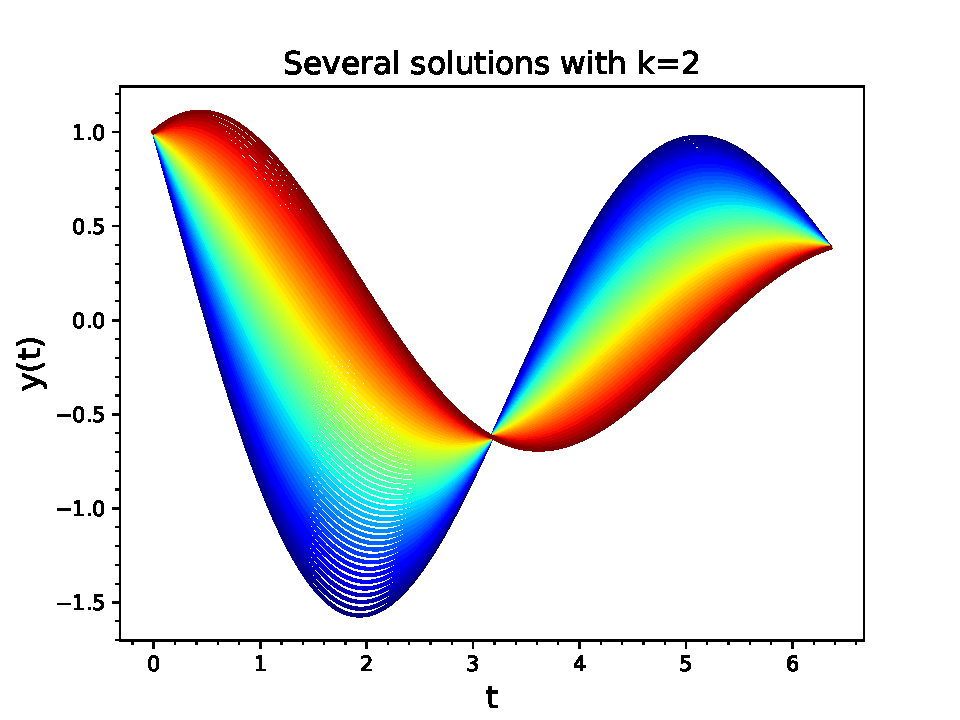
\includegraphics[scale=0.75]{img/BVP_cfr.pdf}
\end{center}

Mi spiace per gli amici daltonici, ma ammetto che questo grafico è stato fatto solo perché bellino vederlo arcobaleno. Come al solito non riportiamo tutto il codice ma solo le due funzioni principali, sia perché il resto del codice non è così istruttivo, sia per invogliarvi a scrivere da voi. In ogni caso però nella cartella sarà presente tutto. \\
Abbiamo detto quindi che ci siamo ricondotti a risolvere una ode come nella sezione di sopra; sfruttiamo l'occasione per introdurre un nuovo metodo di integrazione: un predittore correttore del quarto ordine, Adams-Bashforth-Moulton. Esso fondamentalmente è l'unione di un metodo esplicito, con cui si fa una prima stima della soluzione, la predizione, e poi si inserisce il valore all'interno di un metodo implicito per ottenere il valore finale, la correzione. Detta f la funzione dell'equazione differenziale:
\begin{align}
\overline{y}_{i+1}&=y_i + \frac{h}{24}(55f(t_i,y_i) - 59f(t_{i-1},y_{i-1}) + 37f(t_{i-2},y_{i-2})-9f(t_{i-3},y_{i-3}))\hspace{5 mm} \text{ A.B. predico,}\\
y_{i+1}&=y_i + \frac{h}{24}(9f(t_{i+1},\overline{y}_{i+1})+19f(t_{i},y_{i})-5f(t_{i-1},y_{i-1})+f(t_{i-2},y_{i-2})) \hspace{11.5 mm} \text{A.M. correggo.}
\end{align}
Può ora sorgere un dubbio, come otteniamo i primi tre valori necessari per fare il primo passo di predizione? Dato che si stratta di un integratore di quarto ordine usiamo per i primi tre un Runge-Kutta di ordine 4 che brevemente riportiamo:
\begin{equation}
y_{n+1} = y_n + \frac{h}{6}(k_1 + 2k_2 + 2k_3 + k_4)
\end{equation}
dove:
\begin{align*}
k_1 &= f(t_n, y_n)\\
k_2 &= f(t_n + \frac{h}{2}, y_n + \frac{1}{2} k_1 h)\\
k_3 &= f(t_n + \frac{h}{2}, y_n + \frac{1}{2} k_2 h)\\
k_4 &= f(t_n + h, y_n + k_3 h)
\end{align*}
Passiamo ora al codice:

\begin{lstlisting}[language=Python]
#============================================================================
# Itegration: Adams-Bashforth-Moulton predictor and corretor of order 4
#============================================================================

def AMB4(num_steps, t0, tf, f, init, args=()):
    """
    Integrator with Adams-Bashforth-Moulton
    predictor and corretor of order 4

    Parameters
    ----------
    num_steps : int
        number of point of solution
    t0 : float
        lower bound of integration
    tf : float
        upper bound of integration
    f : callable
        function to integrate, must accept vectorial input
    init : 1darray
        array of initial condition
    args : tuple, optional
        extra arguments to pass to f

    Return
    ------
    X : array, shape (num_steps + 1, len(init))
        solution of equation
    t : 1darray
        time
    """
    #time steps
    dt = tf/num_steps

    X = np.zeros((num_steps + 1, len(init))) #matrice delle soluzioni
    t = np.zeros(num_steps + 1)              #array dei tempi

    X[0, :] = init                           #condizioni iniziali
    t[0]    = t0

    #primi passi con runge kutta
    for i in range(3):
        xk1 = f(t[i], X[i, :], *args)
        xk2 = f(t[i] + dt/2, X[i, :] + xk1*dt/2, *args)
        xk3 = f(t[i] + dt/2, X[i, :] + xk2*dt/2, *args)
        xk4 = f(t[i] + dt, X[i, :] + xk3*dt, *args)
        X[i + 1, :] = X[i, :] + (dt/6)*(xk1 + 2*xk2 + 2*xk3 + xk4)
        t[i + 1] = t[i] + dt

    # Adams-Bashforth-Moulton
    i = 3
    AB0 = f(t[i  ], X[i,   :], *args)
    AB1 = f(t[i-1], X[i-1, :], *args)
    AB2 = f(t[i-2], X[i-2, :], *args)
    AB3 = f(t[i-3], X[i-3, :], *args)

    for i in range(3,num_steps):
        #predico
        X[i + 1, :] = X[i, :] + dt/24*(55*AB0 - 59*AB1 + 37*AB2 - 9*AB3)
        t[i + 1] = t[i] + dt
        #correggo
        AB3 = AB2
        AB2 = AB1
        AB1 = AB0
        AB0 = f(t[i+1], X[i + 1, :], *args)

        X[i + 1, :] = X[i, :] + dt/24*(9*AB0 + 19*AB1 - 5*AB2 + AB3)

    return X, t

#============================================================================
# Binary research to find the right solution with shooting method
#============================================================================

def SH(N, x0, start, xi, xf, step, x1, tau, f, args=()):
    '''
    Function that calculates zeros with the bisection method
    Parameters
    ----------
    N : Integer
        number of integration steps.
    x0 : float
        initial condition on position.
    start : float
        initial condition on speed.
    xi : float
        initial time of integration.
    xf : float
        final time of integration.
    step : float
        start increment
    x1 : float
        boundary condition of solution
    tau : float
        tollerance on find value
    f : callable
        function to integrate, must accept vectorial input
    args : tuple, optional
        extra arguments to pass to f
    Returns
    -------
    m : float
        ideal intial condition for speed
    sol : one dimensional array
        solution of the equation
    '''
    a = start
    sol = AMB4(N, xi, xf, f, init=(x0, a), args=args)
    k = sol[0][-1, 0] - x1
    while True:
        b = a + step
        sol = AMB4(N, xi, xf, f, init=(x0, b), args=args)
        D = sol[0][-1, 0] - x1
        if (k*D)<0.0:
            break
        k = D
        a = b
    while abs(a - b)>tau:
        m = (a + b)/2.0
        sol = AMB4(N, xi, xf, f, init=(x0, m), args=args)
        M = sol[0][-1, 0] - x1
        if (M*k)>0 :
            k = M
            a = m
        else :
            D = M
            b = m
    return m, sol
    
\end{lstlisting}

scegliendo ora come tempo finale $tf = 5$ e il valore al bordo $x1 = 0.1862$, in modo che la soluzione sia unica, otteniamo:

\begin{center}
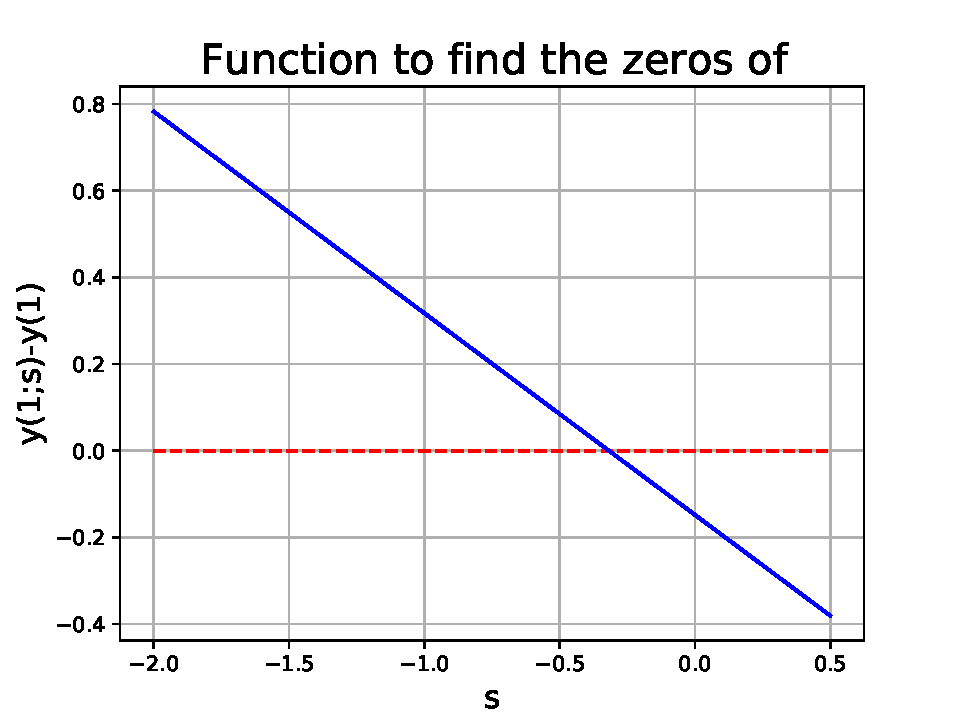
\includegraphics[scale=0.8]{img/zeri_bvp.pdf}
\end{center}

\begin{center}
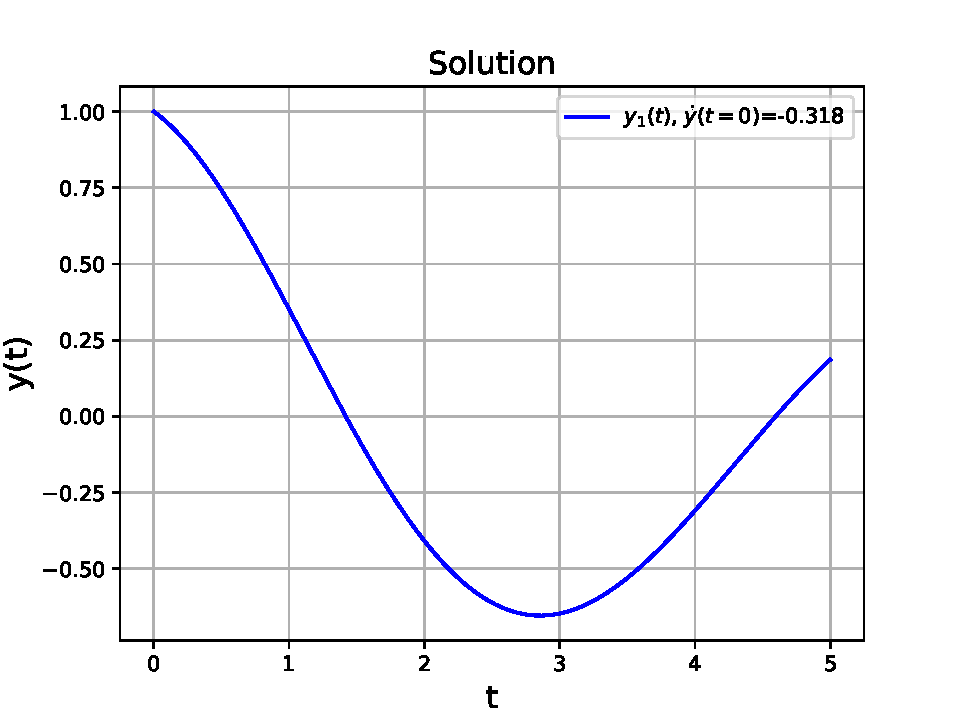
\includegraphics[scale=0.8]{img/sol_bvp.pdf}
\end{center}

\subsection{Relaxation}
Un altro metodo per risolvere equazioni di questo ripo è il metodo di rilassamento, consideriamo come prima, un esempio del tipo precedente:
\begin{equation}
\begin{cases}
\ddot{y}(t) = f(t, y(t), \dot{y}(t))\\
y(t_0)=y_0\\
y(t_1)=y_1
\end{cases}
\end{equation}
Discretizzando la prima equazione abbiamo su una griglia di $N$ punti nella variabile indipendente $t$ abbiamo:
\begin{equation}
\frac{y[i-1] - 2y[i] + y[i+1]}{h^2} = f(x[i], y[i], \frac{y[i-1] - y[i+1]}{2h} ) \quad,
\end{equation}
dove usiamo la derivata simmetrica per avere tutto al secondo ordine; imponendo le condizioni al bordo otteniamo il seguente sistema:
\begin{equation}
P \textbf{y} = f(\textbf{y}) - b \quad,
\end{equation}
in forma matriciale abbiamo
\begin{equation}
\frac{1}{h^2}
\begin{pmatrix}
-2 & 1  & 0 & \cdots &0\\
1  & -2 & 1 & \cdots &0\\
0 & \ddots & \ddots & \ddots &\vdots \\
\vdots & \ddots & 1 &  -2 & 1 \\
0 & \cdots &0&  1 & -2 \\
\end{pmatrix}
\begin{pmatrix}
y[0] \\
y[1] \\
\vdots \\
y[N-1] \\
y[N-2] \\
\end{pmatrix} = 
\begin{pmatrix}
f[0] \\
f[1] \\
\vdots \\
f[N-1] \\
f[N-2] \\
\end{pmatrix}-
\begin{pmatrix}
y_0/h^2 \\
0 \\
\vdots \\
0 \\
y_1/h^2 \\
\end{pmatrix} \quad.
\end{equation}
Però $f$ è una generica funzione quindi fondamentalmente abbiamo un sistema di equazioni non lineare da risolvere nella forma:
\begin{equation}
H(\textbf{y}) = 0 \hspace{5 mm} \text{ con } \hspace{5 mm} H(\textbf{y}) = P \textbf{y} - f(\textbf{y}) + b \quad,
\end{equation}
quindi sappiamo bene che la soluzione la possiamo ottenere linearizzando $H$ con il metodo di newton, si arriva dunque ad un'espressione iterativa:
\begin{equation}
\textbf{y}^{n+1} = \textbf{y}^{n} - \Bigg[ P - \frac{\partial f_i}{\partial y_j} \Bigg]^{-1} [P \textbf{y} - f(\textbf{y}) + b] \quad,
\end{equation}
dove $\frac{\partial f_i}{\partial y_j}$ è lo jacobiano di $f$. Come guess iniziale possiamo provare una funzione generica in linea di principio, certamente più siamo vicini, più il metodo converge senza problemi. La cosa più semplice è una retta che passa per i punti al bordo:
\begin{equation}
y_{\text{initial guess}} = (t - t_0) \frac{y_1 - y_0}{t_1 - t_0} + y_0 \quad.
\end{equation}  
Dove $t$ è il nostro array che va da $t_0$ a $t_1$ in $N$ passi. Scelta la guess, il sistema piano piano rilassa verso la soluzione cercata. Come criterio di stop calcoliamo la distanza tra le soluzioni ad ogni iterazione:
\begin{equation}
R = \sqrt{\sum(\textbf{y}^{n+1} - \textbf{y}^n)^2} \quad,
\end{equation}
se questa quantità è minore di una certa tolleranza allora il programma termina. Vediamo ora il codice:
\begin{lstlisting}[language=Python]
import numpy as np
from scipy.sparse import diags
import  matplotlib.pyplot as plt

#=================================================================================
# Function for the solution of boundary value problem via relaxation
#=================================================================================

def relax(f, y0, y1, x, init, args=(), tol=1e-8, max_iter=100, dense_output=False):
    '''
    Implementation of relaxation method for ODE 2pt-BVP.
    The equation must be in the form: y''(x) = f(x, y, y')
   
    Parameters
    ----------
    f : callable
        A vector function of differential equation like: y'' = f
    y0, y1 : float
        required value of solution at boundary
    x : 1darray
        array of position, or time, independent variable
    init : 1darray 
        Initial guess.
    args : tuple, optional
        Extra arguments passed to f
    tol :float, optional, default 1e-8
        required tollerance
    max_iter : int, optional, default 100
        after max_it iteration the code stop raising an exception
    dense_output : bool, optional, default False
        true for full and number of iteration
    
    Return
    ------
    yo : 1darray
        solution of differential equation
        if dense_outupt=True all iteration are returned
        in a matrix called Y and also the number of iteration
    '''
    # parameter of discretizzation
    N = len(x)
    h = np.diff(x)[0]
    # second derivative matrix
    d2 = diags([1, -2, 1], [-1, 0, 1], shape=(N, N)).toarray()
    d2 = d2/h**2
    # bound values required
    yb = [y0/h**2] + [0]*int(N-2) + [y1/h**2]
    yb = np.array(yb)
    # init guess from imput
    yo = init
    # interation count
    it = 0
    #for full output
    Y = []
    if dense_output : Y.append(yo)
    
    while True:
        # for jacobian computation
        df = np.zeros(d2.shape)
        s  = np.zeros(N)

        for i in range(N):
            s[i] = 1
            yr, yl = yo + h*s, yo - h*s
            df[i, :] = (f(x, yr, h, *args) - f(x, yl, h, *args) )/(2*h)
            s[:] = 0

        yn = yo - np.linalg.solve(d2-df, d2@yo - f(x, yo, h, g, o02) + yb)
        # residual
        R = np.sqrt(np.sum((yn-yo)**2))
        if R < tol:
            yo = yn
            break
            
        if it > max_iter:
            raise Exception("to many iteration")

        #update
        yo = yn
        it = it + 1
        if dense_output : Y.append(yo)
    
    if dense_output:
        return Y, it
    else:
        return yo

#=================================================================================
# RHS of differential equations y'' = f
#=================================================================================

def f(t, y, h, g, o02):
    '''
    RHS of differential equations y'' = f
    f can be a function non only of y but also y' so
    we use a second order approximation to compute y'
    
    Parameter
    ---------
    t : 1darray
        independent variable
    y : 1darray
        solution or guess of solution
    h : float
        step's size for derivative computation
    g, o02 : float
        parameter of our differential equation
    
    Return
    ------
    y_ddot : float
        RHS of equation computed on a grid
    '''
    y_dot   = (y[2:] - y[:-2])/(2*h)              # second order derivative
    y_dot_0 = (- 3*y[0]  + 4*y[1]  - y[2] )/(2*h) # second order derivative on left  bound
    y_dot_n = (  3*y[-1] - 4*y[-2] + y[-3])/(2*h) # second order derivative on right bound
    # join everything together to get the second order derivative
    y_dot = np.insert(y_dot, 0,          y_dot_0)
    y_dot = np.insert(y_dot, len(y_dot), y_dot_n)

    # equation to solve
    y_ddot = -g*y_dot - o02*y

    return y_ddot

#=================================================================================
# Main code and plot
#=================================================================================

g   = 0.3    # damping factor
o02 = 1      # proper frequency squared
xi  = 0      # left  end of the interval
xf  = 5      # right end of the interval
N   = 1000   # number of points
y0  = 1      # boundary condition on xi
y1  = 0.1862 # boundary condition on xf

x = np.linspace(xi, xf, N)
y = (x - xi) * (y1 - y0)/(xf - xi) + y0 # linear guess

Y, n = relax(f, y0, y1, x, y,args=(g, o02), dense_output=True)
print(f"{n} iterations required")

for y in Y:
    plt.plot(x, y)

plt.title("Solution via relaxation method", fontsize=15)
plt.xlabel("x", fontsize=15)
plt.ylabel("y", fontsize=15)
plt.grid()
plt.show()

[Output]
30 iterations required
\end{lstlisting}

\begin{center}
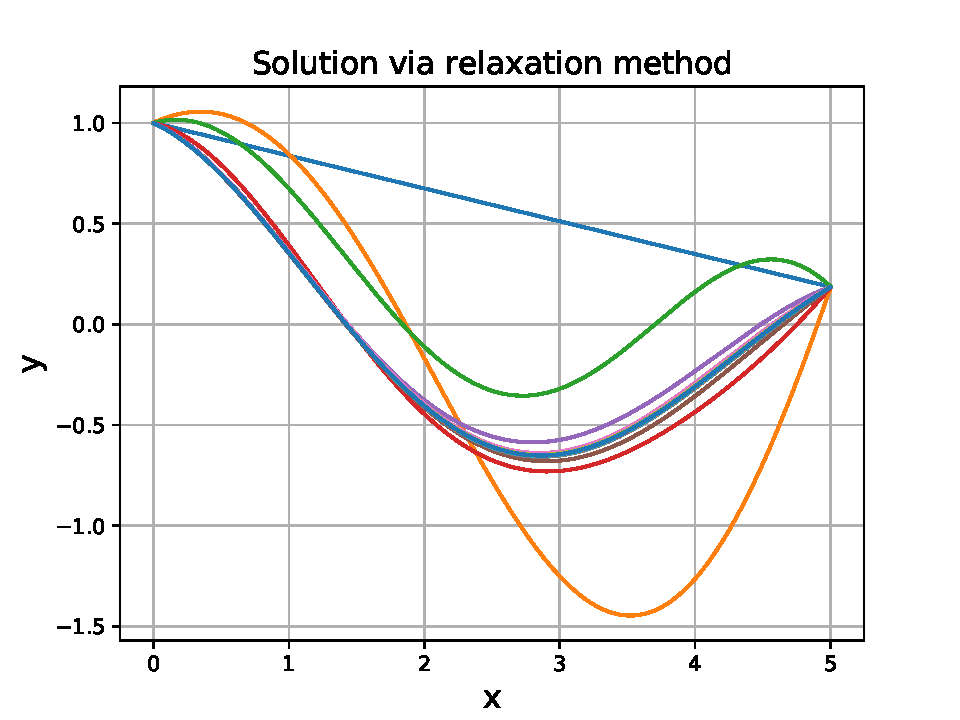
\includegraphics[scale=0.8]{img/BVP_relax.pdf}
\end{center}




\newpage

\section{Sistemi lineari}
Spesso capita, come abbiamo visto sopra con il caso dei fit,  di dover risolvere dei sistemi di equazioni o di invertire una matrice.
Abbiamo un sistema del tipo:
\begin{equation}
A x = b
\end{equation}
dove 
\[
A = \begin{bmatrix} 
a_{11} & a_{12} & \cdots & a_{1n} \\
a_{21} & a_{22} & \cdots & a_{2n} \\
\vdots & \vdots & \ddots & \vdots \\
a_{n1} & a_{n2} & \cdots & a_{nn}
\end{bmatrix}, 
\qquad  
x = \begin{bmatrix} x_{1} \\ x_2 \\ \vdots \\ x_n \end{bmatrix} ,
\qquad
b = \begin{bmatrix} b_{1} \\ b_2 \\ \vdots \\ b_n \end{bmatrix}
\]
\subsection{Metodo Gauss–Seidel}
Detta $L$ una matrice triangolare inferiore e $U$ matrice triangolare superiore, con diagonale nulla tale che $A = L + U$

\begin{equation}
L = 
\begin{bmatrix} 
a_{11} & 0 & \cdots & 0 \\ 
a_{21} & a_{22} & \cdots & 0 \\
\vdots & \vdots & \ddots & \vdots \\
a_{n1} & a_{n2} & \cdots & a_{nn} 
\end{bmatrix}
\qquad
U = 
\begin{bmatrix}
0 & a_{12} & \cdots & a_{1n} \\
0 & 0 & \cdots & a_{2n} \\
\vdots & \vdots & \ddots & \vdots \\
0 & 0 & \cdots & 0 
\end{bmatrix}
\end{equation}
Allora abbiamo:
\begin{align}
A x &= b \\
(L + U) x &= b \\
L x + U x &= b \\
L x &= b - U x
\end{align}
e quindi abbiamo in maniera iterativa:
\begin{equation}
x^{k+1} = L^{-1} (b - U x^{k})
\end{equation}
e per la riga i-esima di $x^{k+1}$ possiamo scrivere:
\begin{equation}
x^{k+1}_i  = \frac{1}{a_{ii}} \Bigg(b_i - \sum_{j=1}^{i-1}a_{ij}x^{k+1}_j - \sum_{j=i+1}^{n}a_{ij}x^{k}_j \Bigg)
\end{equation}
Questo metodo converge solo per alcune caratteristiche della matrice $A$: $A$ deve essere simmetrica definita positiva, oppure deve essere dominante diagonale ($|a_{ii}| \geq \sum_{j\neq i} |a_{ij}| \quad \forall i)$. Esiste una vesrione modificata di questo metodo chiamata: successive over-relaxation (SOR)

\subsection{Successive over-relaxation}
Se ora scomponiamo $A$ come $D + L + U$:
\begin{equation}
D = 
\begin{bmatrix}
a_{11} & 0 & \cdots & 0 \\
0 & a_{22} & \cdots & 0 \\
\vdots & \vdots & \ddots & \vdots \\
0 & 0 & \cdots & a_{nn}
\end{bmatrix}
\qquad 
L = 
\begin{bmatrix} 0 & 0 & \cdots & 0 \\
a_{21} & 0 & \cdots & 0 \\
\vdots & \vdots & \ddots & \vdots \\
a_{n1} & a_{n2} & \cdots & 0 
\end{bmatrix}
\qquad
U = 
\begin{bmatrix}
0 & a_{12} & \cdots & a_{1n} \\
0 & 0 & \cdots & a_{2n} \\
\vdots & \vdots & \ddots & \vdots \\
0 & 0 & \cdots & 0
\end{bmatrix}
\end{equation}
Introducendo il parametro $\omega$ di overrelaxation l'algoritmo diventa:
\begin{equation}
x^{k+1}_i  = (1 - \omega) x_i^k +  \frac{\omega}{a_{ii}} \Bigg(b_i - \sum_{j=1}^{i-1}a_{ij}x^{k+1}_j - \sum_{j=i+1}^{n}a_{ij}x^{k}_j \Bigg)
\end{equation}
Vediamo quindi che per $\omega=1$ recuperiamo il metodo precedente. Vediamo ora un esempio di codice e vedremo che due esecuzioni con $\omega$ diversi cambiano molto. In particolare $0 < \omega < 2$ e valori più vicini a due ne migliorano la convergenza.

\begin{lstlisting}[language=Python]
import time
import numpy as np

def SOR(A, b, omg, tol=1e-6):
    """
    Implementation of successive over-relaxation method for solve A @ x = b;
    A must be:
    1) symmetric (i.e. A.T = A)
    2) positive-definite (i.e. x.T@A@x > 0 for all non-zero x)
    3) real.

    Parameters
    ----------
    A : 2darray
        matrix of system.
    b : 1darray
        Ordinate or dependent variable values.
    tol : float, optional
        required tollerance default 1e-6

    Return
    ------
    x : 1darray
        solution of system
    iter : int
        number of iteration
    """
    x = np.zeros(len(b))
    iter = 0
    while True:

        x_new = np.zeros(len(x))

        for i in range(A.shape[0]):
            s1 = np.dot(A[i, :i], x_new[:i])
            s2 = np.dot(A[i, i + 1:], x[i + 1:])
            x_new[i] = (1 - omg)*x[i] + omg*(b[i] - s1 - s2) / A[i, i]

        res = np.sqrt(np.sum((A @ x_new - b)**2))
        if res < tol:
            break

        x = x_new
        iter += 1

    return x, iter

if __name__ == "__main__":
    np.random.seed(69420)
    N = 20
    A = np.random.normal(size=[N, N])
    A = A.T @ A #per garantire la convergenza del metodo
    b = np.random.normal(size=[N])

    start = time.time()
    x1, iter = SOR(A, b, 1.9, 1e-8)
    print(f"number of iteration = {iter}")
    print(f"Elapsed time = {time.time()-start}")

    start = time.time()
    x2 = np.linalg.solve(A, b)
    print(f"Elapsed time = {time.time()-start}")

    d = np.sqrt(np.sum((x1 - x2)**2))
    print(f'difference with numpy = {d}')

[Output] (omg=1)
number of iteration = 10794
Elapsed time = 1.4843645095825195
Elapsed time = 0.0
difference with numpy = 4.5979072526656344e-07

[Output] (omg=1.9)
number of iteration = 2590
Elapsed time = 0.35565781593322754
Elapsed time = 0.0
difference with numpy = 2.1632731207202056e-08
\end{lstlisting}

\subsection{Metodo del gradiente coniugato}
Un altro modo per risolvere sistemi lineari, e che ci permettere di far crescere la dimensione dalla matrice, è il metodo del gradiente coniugato. La matrice $A$ come sopra deve essere definita positiva.
L'algoritmo è iterativo e l'aggiornamento della posizione è fatto secondo la seguente regola:
\begin{equation}
x_{k+1} = x_k + \alpha_k p_k
\end{equation}  
dove $p_k$ è la direzione di discesa ed è scelto in modo che sia ortogonale rispetto al prodotto scalare indotto da $A$ : $ \langle p_j, p_k\rangle_A = 0,\, \forall j=0,\dots,k-1$. Mentre $\alpha_k$ è la grandezza del passo, $\frac{p_k^T r_k}{p_k^T A p_k}$. Vediamone l'implementazione:

\begin{lstlisting}[language=Python]
"""
Implementation and test for
conjugate gradient method
"""

import time
import numpy as np
import matplotlib.pyplot as plt
from scipy.sparse.linalg import cg


def conj_grad(A, b, tol=1e-6, dense_output=False):
    """
    Implementation of conjugate gradient method for solve A @ x = b
    A must be:
    1) symmetric (i.e. A.T = A)
    2) positive-definite (i.e. x.T @ A @ x > 0 for all non-zero x)
    3) real.

    Parameters
    ----------
    A : 2darray
        matrix of system.
    b : 1darray
        Ordinate or dependent variable values.
    tol : float, optional
        required tollerance default 1e-6
    dense_output : bool, optional
        if True all iteration of th solution, error and number
        of iteration are stored and reurned, default is False

    Return
    ------
    x : 1darray
        solution of system
    err : float
        error of solution

    if dense_output :
    s : 2darray
        all iteration of solution
    e : 1darray
        error of all iteration,
    iter : int
        number of iteration

    """

    N = len(b)
    x = np.zeros(N) #initia guess

    r = b - A @ x   #residuals
    p = r           #descent direction
    r2 = sum(r*r)   #norm^2 residuals

    if dense_output:
        s = []
        e = []
        s.append(x)
        e.append(np.sqrt(r2))

    iter = 0

    while True:

        Ap = A @ p            #computation of
        alpha = r2 /(p @ Ap)  #descent's step

        x = x + alpha * p     #updare position
        r = r - alpha * Ap    #update residuals

        r2_new = sum(r*r)     #norm^2 new residuals
        beta = r2_new/r2      #compute step for p

        r2 = r2_new   #update norm

        if dense_output:
            s.append(x)
            e.append(np.sqrt(r2))

        if np.sqrt(r2_new) < tol : #break condition
            break

        p = r + beta * p   #update p
        iter += 1

    if not dense_output:
        err = np.sqrt(r2_new)
        return x, err
    else:
        return np.array(s), np.array(e), iter


if __name__ == '__main__':

    np.random.seed(69420)

    N = 1000
    P = np.random.normal(size=[N, N])
    A = np.dot(P.T, P) #deve essere simmetrica e semidef >0
    b = np.random.normal(size=[N])

    t1 = time.time()
    sol, err, iter = conj_grad(A, b, 1e-8, dense_output=True)
    x1 = sol[-1]
    t2 = time.time()
    print(f'numero di iterazioni: {iter}')
    print(f'Elapsed time       = {t2 - t1}')

    t1 = time.time()
    x2 = np.linalg.solve(A, b)
    t2 = time.time()
    print(f'Elapsed time numpy = {t2 - t1}')

    t1 = time.time()
    x3, exit_code = cg(A, b)
    t2 = time.time()
    print(f'Elapsed time scipy = {t2 - t1}')

    print('confronto soluzioni')
    print(f"distanza delle due soluzioni(cg-n) = {np.sqrt(np.sum((x1-x2)**2))}")
    print(f"distanza delle due soluzioni(cg-s) = {np.sqrt(np.sum((x1-x3)**2))}")


    plt.figure(1)
    plt.grid()
    plt.plot(abs(err))
    plt.xlabel('iteration')
    plt.ylabel('error')
    #plt.xscale('log')
    plt.yscale('log')
    plt.show()

[Output]
numero di iterazioni: 1916
Elapsed time       = 1.2752277851104736
Elapsed time numpy = 0.03131294250488281
Elapsed time scipy = 1.1133522987365723
confronto soluzioni
distanza delle due soluzioni(cg-n) = 3.295292002340236e-08
distanza delle due soluzioni(cg-s) = 5.375356794116895e-07
\end{lstlisting}
Come è possibile vedere ne abbiamo guadagnato molto con questo metodo, risulta essere più veloce e non fatica non matrici molto grosse.





\newpage


\section{Risolvere numericamente le PDE}
Come si diceva sopra sono tantissimi i fenomeni fisici che sono descritti da un'equazione differenziale alle derivate parziali, e per non dilungarci nella trattazione, tratteremo solo due esempi: equazione del trasporto ed equazione del calore (per dimensioni 1+1), che possono essere viste come casi specifici della stessa equazione. I metodi che vedremmo, sempre per dare giusto un'infarinatura e lasciare molto all'approfondimento personale, sono l'FCTS (forward time centered space) e il metodo di Lax. I metodi sono entrambi espliciti, ovvero non richiedono la risoluzione di un'equazione algebrica, o di un sistema di equazioni. Sono presenti nei codici delle animazioni per meglio visualizzare la soluzione:

\subsection{Equazione del trasporto}
L'equazione di nostro interesse è:
\[
\frac{\partial u}{\partial t} + v\frac{\partial u}{\partial x}=0
\]
ovviamente ci serve una condizione iniziale $u(x,t=0)$ per far evolvere il sistema. Per risolverlo si potrebbe pensare il metodo di eulero (notazione: gli apici indicano la dipendenza temporale i pedici quella spaziale) :
\[
\frac{u^{n+1}_j - u^n_j}{\Delta t} = - v \frac{u^{n}_{j+1} - u^n_{j-1}}{2 \Delta x}
\]
dove per approssimare la derivata nello spazio si è utilizzata il metodo delle differenze centrali, più preciso, poiché date le condizioni iniziali sappiamo la soluzione per ogni x ad un dato tempo. Se però per le ode il metodo di Eulero, detto per le PDE: FCTS, funziona praticamente sempre, già in questo esempio il metodo fallisce. Per vederlo si esegue quella che è un'analisi di stabilità, ovvero si sostituisce nella formula di sopra una soluzione del tipo $u^n_j=\xi^n \exp{ikj \Delta x}$ e si vede che l'ampiezza $\xi$ diverge per ogni scelta di $\Delta t $ e $\Delta x$ per risolvere si può usare il metodo di Lax nel quale in termine $u^n_j$ viene sostituito dalla media dei punti spaziali immediatamente accanto:
\[
u^{n+1}_j = \frac{u^{n}_{j+1} + u^n_{j-1}}{2} - v \Delta t \frac{u^{n}_{j+1} - u^n_{j-1}}{2 \Delta x}
\]
Ora il metodo è stabile se $\frac{v \Delta t}{\Delta x}<1$ \\

\begin{lstlisting}[language=Python]
import numpy as np
import matplotlib.pyplot as plt
import matplotlib.animation as animation

N = 100	    #numero punti sulle x
T = 400	    #numero di punti nel tempo
v = 1       #velocita' di propagazione
dt = 0.001  #passo temporale
dx = 0.01   #passo spaziale 

alpha = v*dt/dx #<1
print(alpha)

Sol = np.zeros((N+1, T))
sol_v = np.zeros(N+1)
sol_n = np.zeros(N+1)

#condizione iniziale
q = 2*np.pi
x = np.linspace(0, (N+1)*dx, N+1)
sol_v = np.sin(q*1*x)
Sol[:, 0] = sol_v

#evoluzione temporale con lax
for time in range(1, T):
    for j in range(1, N):
        sol_n[j] = 0.5*(sol_v[j+1]*(1 - alpha)) + 0.5*(sol_v[j-1]*(1 + alpha))
      
    #condizione periodiche al bordo  
    sol_n[0] = sol_n[N-1]
    sol_n[N] = sol_n[1]
    
    #aggiorno la soluzione
    sol_v = sol_n
    
    #conservo la soluzione per l'animazione
    Sol[:, time] = sol_v
    
    
fig = plt.figure(1)
ax = fig.add_subplot(projection='3d')
ax.set_title('Equazione trasporto con Lax')
ax.set_ylabel('Distanza')
ax.set_xlabel('Tempo')
ax.set_zlabel('Ampiezza')

gridx, gridy = np.meshgrid(range(T), x)
ax.plot_surface(gridx, gridy, Sol)

plt.figure(2)

plt.title('Animazione soluzione', fontsize=15)
plt.xlabel('distanza')
plt.ylabel('ampiezza')
plt.grid()
plt.xlim(np.min(x), np.max(x))
plt.ylim(np.min(Sol[:,0]) - 0.1, np.max(Sol[:,0]) + 0.1)

line, = plt.plot([], [], 'b-')

def animate(i):
    
    line.set_data(x, Sol[:, i])
    return line,

anim = animation.FuncAnimation(fig, animate, frames=np.arange(0, T, 1) ,interval=10, blit=True, repeat=True)

plt.show()
\end{lstlisting}
Eseguendo il codice è possibile vedere che l'ampiezza dell'onda iniziale va diminuendo, cosa che guardando l'equazione non ci aspetteremmo; ciò è dovuto al fatto che il metodo di Lax può essere visto come un FCTS di un'equazione con un termine diffusivo, ovvero un termine di derivata seconda stile equazione del calore. Vi è quindi un problema di diffusione numerica. Possiamo però risolverlo utilizzando un altro metodo, quello di Lax-Wendroff.

\subsection{Equazione del calore}
L'equazione del calore è:
\[
\frac{\partial u}{\partial t} - D\frac{\partial^2 u}{\partial x^2}=0
\]
Questa volta si può vedere che lo schema FCTS è stabile:
\[
u^{n+1}_j = u^{n}_j + \frac{D \Delta t}{2 \Delta x^2} (u^n_{j+1} - 2u^n_j + u^n_{j-1})
\]
La condizione di stabilità è: $\frac{D \Delta t}{\Delta x^2} < \frac{1}{2}$

\begin{lstlisting}[language=Python]
import numpy as np
import matplotlib as mp
import matplotlib.pyplot as plt
import matplotlib.animation as animation

N = 100 #punti sulle x
x = np.linspace(0, N, N)
tstep = 5000 #punti sul tempo
T = np.zeros((N,tstep))

#Profilo di temperatura iniziale
T[0:N,0] = 500*np.exp(-((50-x)/20)**2)

D = 0.5
dx = 0.01
dt = 1e-4
r = D*dt/dx**2
#r < 1/2 affinche integri bene
print(r)

for time in range(1,tstep):
    for i in range(1,N-1):
        T[i,time]=T[i,time-1] + r*(T[i-1,time-1]+T[i+1,time-1]-2*T[i,time-1])
#    T[0,time]=T[1,time] #per avere bordi non fissi
#    T[N-1,time]=T[N-2,time]

fig = plt.figure(1)
ax = fig.gca(projection='3d')
gridx, gridy = np.meshgrid(range(tstep), range(N))
ax.plot_surface(gridx,gridy,T, cmap=mp.cm.coolwarm,vmax=250,linewidth=0,rstride=2, cstride=100)
ax.set_title('Diffusione del calore')
ax.set_xlabel('Tempo')
ax.set_ylabel('Lunghezza')
ax.set_zlabel('Temperatura')

fig = plt.figure(2)
plt.xlim(np.min(x), np.max(x))
plt.ylim(np.min(T), np.max(T))

line, = plt.plot([], [], 'b')
def animate(i):
    line.set_data(x, T[:,i])
    return line,


anim = animation.FuncAnimation(fig, animate, frames=tstep, interval=10, blit=True, repeat=True)

plt.grid()
plt.title('Diffusione del calore')
plt.xlabel('Distanza')
plt.ylabel('Temperatura')

#anim.save('calore.mp4', fps=30, extra_args=['-vcodec', 'libx264'])

plt.show()
\end{lstlisting}

\newpage

\section{Presa dati da foto}
Può capitare che sia interessante prendere dei dati da analizzare, in un qualche modo o maniera, da una foto. Riportiamo quindi un semplice codice che permettere di aprire una foto e salvare su file.txt le coordinate dei pixel, tutto ciò semplicemente cliccando sulla foto (Ogni click che si effettua sulla foto vengono lette e salvate le coordinate del pixel cliccato).


\begin{lstlisting}[language=Python]
import matplotlib as mp
import matplotlib.pyplot as plt


#il file txt su cui scrivere se non esiste viene creato automaticamente

path_dati = "C:\\Users\\franc\\Desktop\\dati0.txt"
path_img = "C:\\Users\\franc\\Documents\\DatiL\\datiL3\\FIS2\\eOverm\\DSC_0005.jpg"

fig, ax = plt.subplots()

img = mp.image.imread(path_img)

ax.imshow(img)


def onclick(event):
    #apre file, il permesso e' a altrimenti sovrascriverebbe i dati
    file= open(path_dati, "a")

    x=event.xdata
    y=event.ydata
    print('x=%f, y=%f' %(x, y)) #stampa i dati sulla shell

    #scrive i dati sul file belli pronti per essere letti da codice del fit
    file.write(str(x))
    file.write('\t')
    file.write(str(y))
    file.write('\n')
    file.close() #chiude il file


fig.canvas.mpl_connect('button_press_event', onclick)


plt.show()

\end{lstlisting}

\newpage

\section{Fit}
Illustriamo brevemente alcuni modi di eseguire dei fit numerici, cosa in generale in fisica molto utile poiché ci permette di determinare se i dati seguano o meno un certo andamento predetto dalla teoria.
\subsection{Fit con scipy}
La libreria scipy grazie alla funzione "curve\_fit()" ci permette di eseguire un gran numero di fit; riportiamo sotto un esempio di codice e relativi risultati e grafico:

\begin{lstlisting}[language=Python]
import numpy as np
import matplotlib.pyplot as plt
from scipy.optimize import curve_fit

#Importiamo i dati (va inserito il path assoluto per permettere di trovare) e definiamo la funzione di fit:
#x, y= np.loadtxt(r'C:\Users\franc\Desktop\datiL\DatiL2\onda.txt', unpack = True)
N = 500
ex, ey = 0.1, 1
dy = np.array(N*[ey])
dx = np.array(N*[ex])
x = np.linspace(0, 50, N)

A1 = 20
o1 = 2
v1 = 30
phi = np.pi/4

y = A1*np.sin(o1*x + phi) + v1
k = np.random.uniform(0, ey, N)
l = np.random.uniform(0, ex, N)
y = y + k #aggiungo errore
x = x + l

def f(x, A, o, f, v):
    '''funzione modello
    '''
    return A*np.sin(o*x + f) + v

"""
definiamo un array di parametri iniziali contenente
i volori numerici che ci si aspetta il fit restituisca,
per aiutare la convergenza dello stesso:
init = np.array([A, o, f, v])
"""
init = np.array([25, 2.1, 3, 29])


#Eseguiamo il fit e stampiamo i risultati:
pars, covm = curve_fit(f, x, y, init, sigma=dy, absolute_sigma=False)
print('A  = %.5f +- %.5f ' % (pars[0], np.sqrt(covm.diagonal()[0])))
print('o  = %.5f +- %.5f ' % (pars[1], np.sqrt(covm.diagonal()[1])))
print('f  = %.5f +- %.5f ' % (pars[2], np.sqrt(covm.diagonal()[2])))
print('v  = %.5f +- %.5f ' % (pars[3], np.sqrt(covm.diagonal()[3])))

#Calcoliamo il chi quadro,indice ,per quanto possibile, della bonta' del fit:
chisq = sum(((y - f(x, *pars))/dy)**2.)
ndof = len(y) - len(pars)
print(f'chi quadro = {chisq:.3f} ({ndof:d} dof)')


#Definiamo un matrice di zeri che divvera' la matrice di correlazione:
c=np.zeros((len(pars),len(pars)))
#Calcoliamo le correlazioni e le inseriamo nella matrice:
for i in range(0, len(pars)):
    for j in range(0, len(pars)):
       c[i][j] = (covm[i][j])/(np.sqrt(covm.diagonal()[i])*np.sqrt(covm.diagonal()[j]))
print(c) #matrice di correlazione


#Grafichiamo il risultato
fig1 = plt.figure(1)
#Parte superiore contenetnte il fit:
frame1=fig1.add_axes((.1,.35,.8,.6))
#frame1=fig1.add_axes((trasla lateralmente, trasla verticamente, larghezza, altezza))
frame1.set_title('Fit dati simulati',fontsize=20)
plt.ylabel('ampiezza [u.a.]',fontsize=10)
#plt.ticklabel_format(axis = 'both', style = 'sci', scilimits = (0,0))#notazione scientifica sugliassi
plt.grid()

#grafichimao i punti e relative barre d'erroe
plt.errorbar(x, y, dy, dx, fmt='.', color='black', label='dati') 
t = np.linspace(np.min(x),np.max(x), 10000)
s = f(t, *pars)
plt.plot(t,s, color='blue', alpha=0.5, label='best fit') #grafico del best fit
plt.legend(loc='best')#inserisce la legenda nel posto migliorte


#Parte inferiore contenente i residui
frame2=fig1.add_axes((.1,.1,.8,.2))

#Calcolo i residui normalizzari
ff = (y-f(x, *pars))/dy
frame2.set_ylabel('Residui Normalizzati')
plt.xlabel('tempo [u.a.]',fontsize=10)
#plt.ticklabel_format(axis = 'both', style = 'sci', scilimits = (0,0))


plt.plot(t, 0*t, color='red', linestyle='--', alpha=0.5) #grafico la retta costantemente zero
plt.plot(x, ff, '.', color='black') #grafico i residui normalizzati
plt.grid()

plt.show()

[Output]
A  = 19.95561 +- 0.05547 
o  = 1.99991 +- 0.00019 
f  = 6.96973 +- 0.00565 
v  = 30.54562 +- 0.03930 
chi quadro = 382.795 (496 dof)
[[ 1.          0.00576834 -0.00302643  0.00468354]
 [ 0.00576834  1.         -0.86984711 -0.02110156]
 [-0.00302643 -0.86984711  1.          0.02174393]
 [ 0.00468354 -0.02110156  0.02174393  1.        ]]
 
\end{lstlisting}
\begin{center}
\makebox[\textwidth][c]{
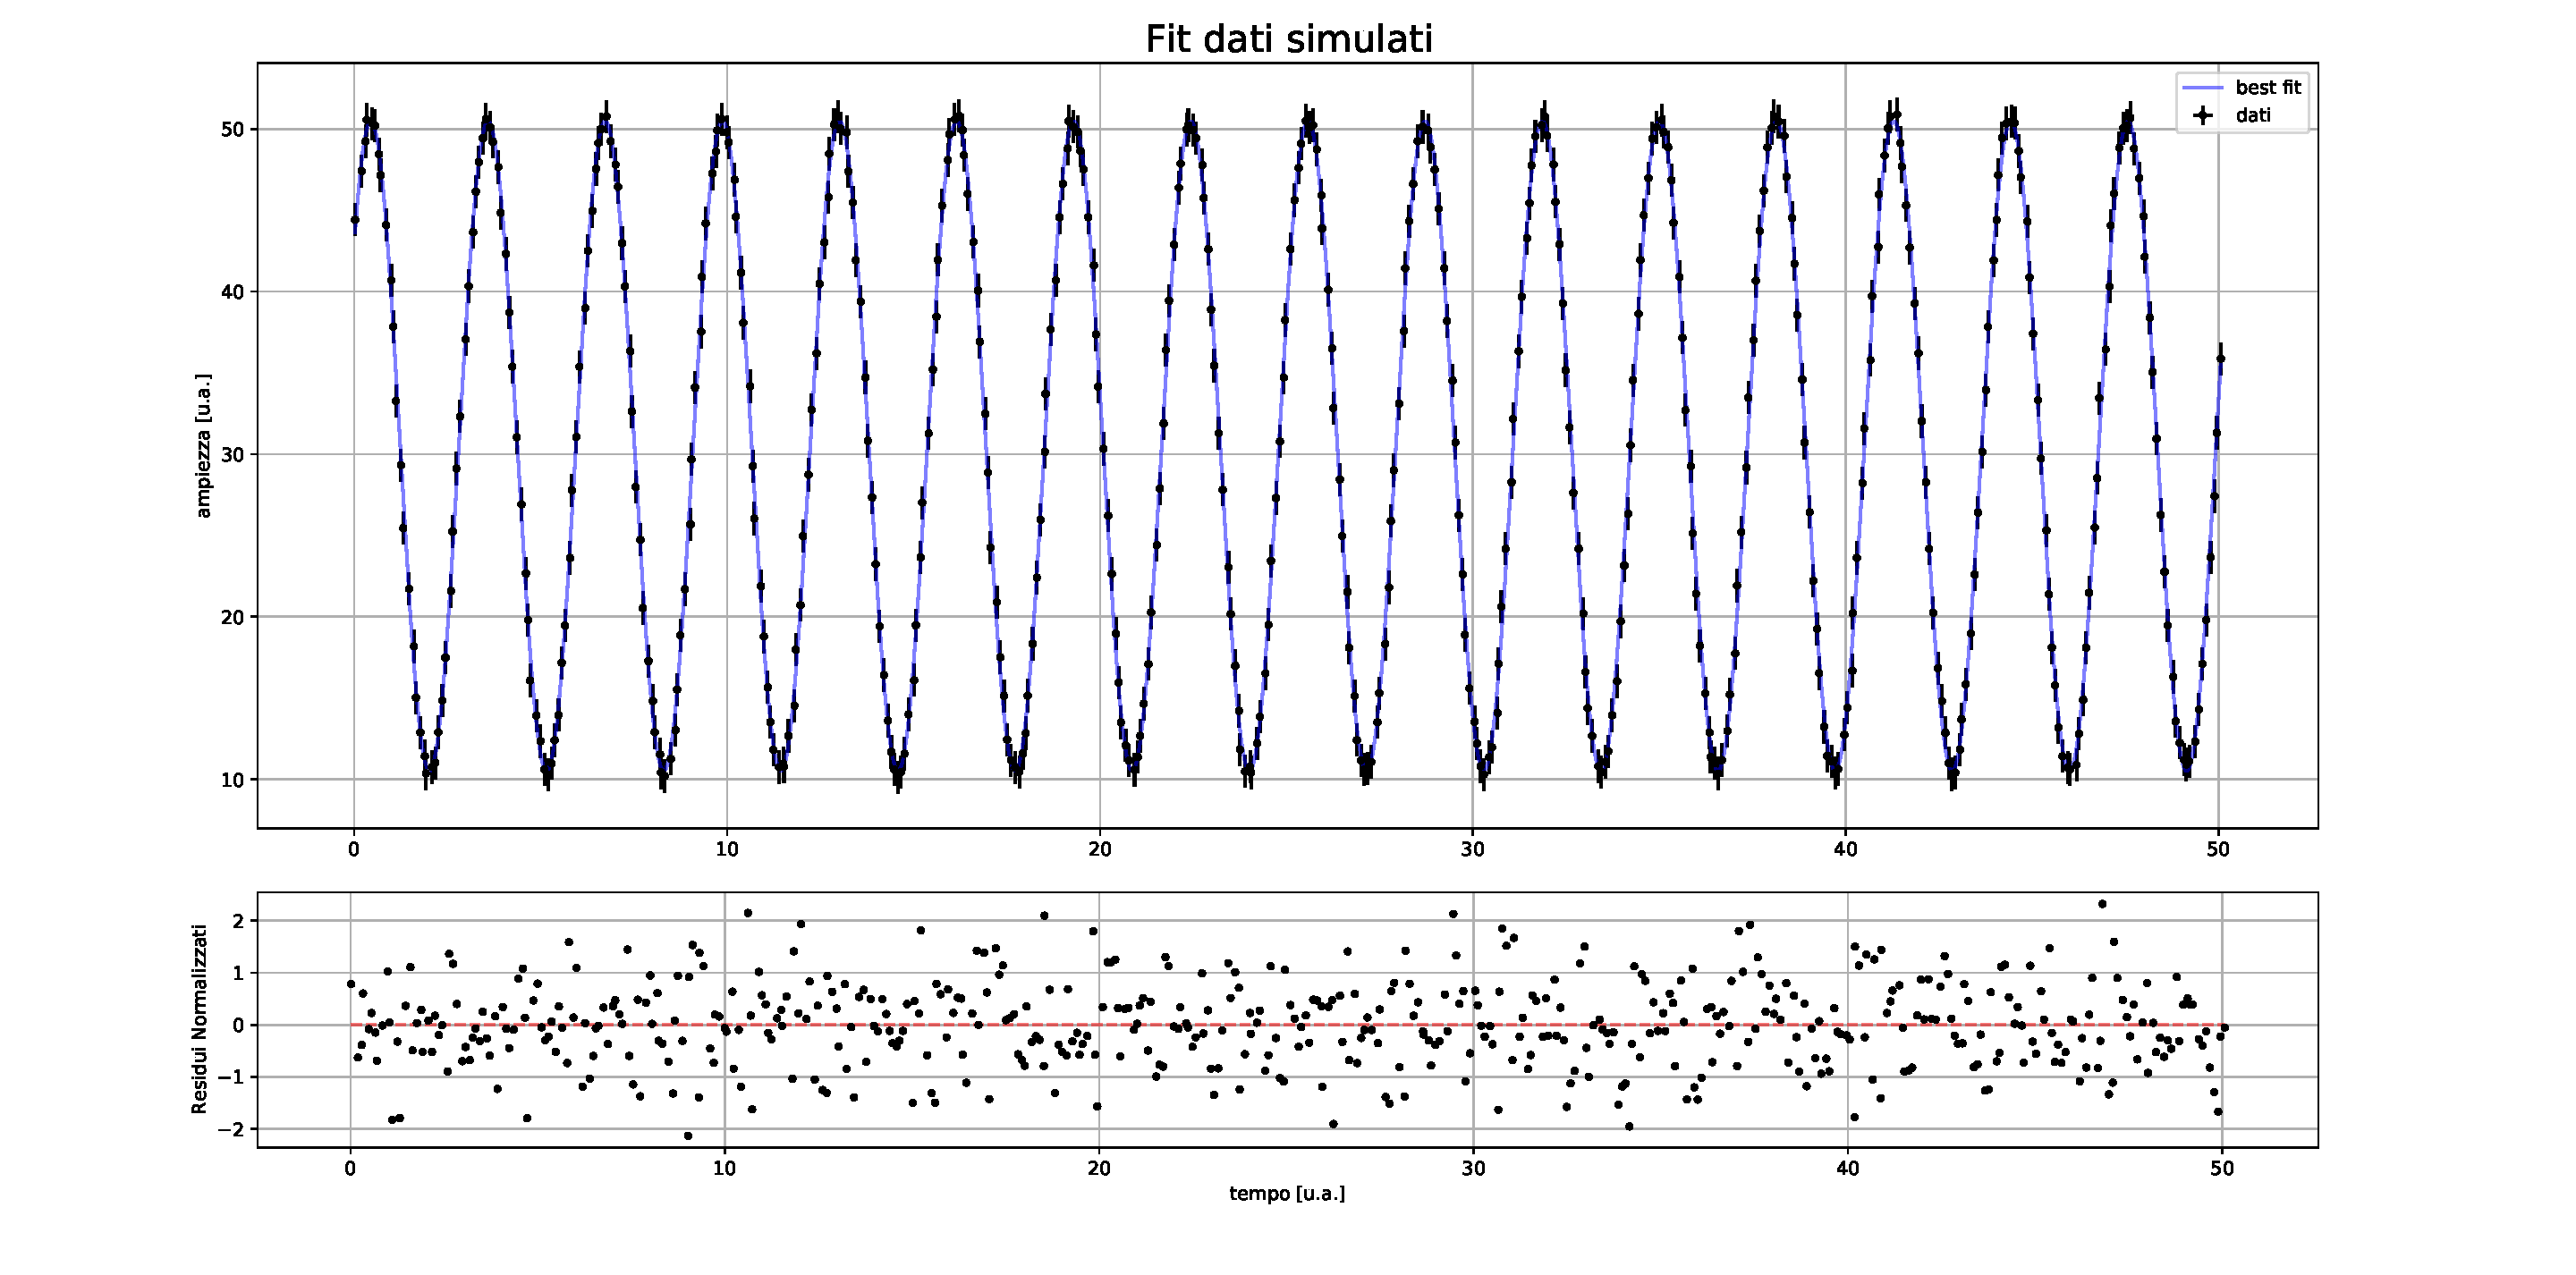
\includegraphics[scale=0.4]{img/fit_scipy.pdf}
}
\end{center}

\newpage
\subsection{Fit circolare,  metodo di Coope}
Ci sono casi in cui, come per un circonferenza o un'ellisse, curve fit non è comodo da usare, in quanto non si tratta di vere e proprie funzioni. Mostriamo un esempio di fit circolare seguito con il metodo di Coope e riportiamo qui il link all'articolo originale: \url{https://core.ac.uk/download/pdf/35472611.pdf}
\begin{lstlisting}[language=Python]
import numpy as np
import matplotlib.pyplot as plt


def cerchio(xc, yc, r, N, phi_min=0, phi_max=2*np.pi):
    """
    Restituisce un cerchio di centro (xc, yc) e di raggio r
    phi e' il parametro di percorrenza del cerchio
    """

    phi = np.linspace(phi_min, phi_max, N)

    x = xc + r*np.cos(phi)
    y = yc + r*np.sin(phi)

    return x, y


def fitcerchio(pt, w=None):
    '''
    fit di un cerchio con metodo di coope
    Parameters
    ----------
    pt : 2Darray
        contiene le coordinate del cerchio
    w : None or 1Darray
        w = np.sqrt(dx**2 + dy**2)
        if None => w = np.ones(len(pt[0]))


    Returns
    -----------
    c : 1Darray
        array con le coordinate del centro del cerchio
    r : float
        raggio del cerchio
    d : 1Darray
        array con gli errori associati a c ed r
    A1 : 2Darray
        matrice di covarianza
    '''
    npt = len(pt[0])

    S = np.column_stack((pt.T, np.ones(npt)))
    y = (pt**2).sum(axis=0)

    if w is None:
        w = np.ones(npt)

    w = np.diag(1/w)

    A = S.T @ w @ S #@ -> prodotto matriciale
    b = S.T @ w @ y
    sol = np.linalg.solve(A, b)

    c = 0.5*sol[:-1]
    r = np.sqrt(sol[-1] + c.T @ c)

    d = np.zeros(3)
    A1 = np.linalg.inv(A)

    for i in range(3):
        d[i] = np.sqrt(A1[i,i])
    return c, r, d, A1


if __name__ == "__main__":
    np.random.seed(69420)
    #numero di punti
    N = 50
    #paramentri cerchio
    xc, yc, r1 = 5, -2, 10
    #errori
    ex, ey = 0.5, 0.5
    dy = np.array(N*[ey])
    dx = np.array(N*[ex])
    dr = np.sqrt(dx**2 + dy**2)
    k = np.random.uniform(0, ex, N)
    l = np.random.uniform(0, ey, N)
    #creiamo il cerchio
    x, y = cerchio(xc, yc, r1, N, np.pi/4, 5/3*np.pi)
    x = x + k #aggiungo errore
    y = y + l

    a = np.array([x, y])
    c, r, d , A = fitcerchio(a, dr) #fit

    print(f'x_c = {c[0]:.5f} +- {d[0]:.5f}; valore esatto = {xc:.5f}')
    print(f'y_c = {c[1]:.5f} +- {d[1]:.5f}; valore esatto = {yc:.5f}')
    print(f'r   = {r:.5f} +- {d[2]:.5f}; valore esatto = {r1:.5f}')


    chisq = sum(((np.sqrt((x-c[0])**2 + (y-c[1])**2) - r)/dr)**2.)
    ndof = N - 3
    print(f'chi quadro = {chisq:.3f} ({ndof:d} dof)')

    corr=np.zeros((3,3))
    for i in range(0, 3):
        for j in range(0, 3):
            corr[i][j]=(A[i][j])/(np.sqrt(A.diagonal()[i])*np.sqrt(A.diagonal()[j]))
    print(corr)

    #plot
    fig1 = plt.figure(1, figsize=(7.5,9.3))
    frame1=fig1.add_axes((.1,.35,.8,.6))
    #frame1=fig1.add_axes((trasla lateralmente, trasla verticamente, larghezza, altezza))
    frame1.set_title('Fit dati simulati',fontsize=20)
    plt.ylabel('y [a.u]',fontsize=10)
    plt.grid()

    plt.errorbar(x, y, dy, dx, fmt='.', color='black', label='dati')
    xx, yy = cerchio(c[0], c[1], r, 10000)
    plt.plot(xx, yy, color='blue', alpha=0.5, label='best fit')
    plt.legend(loc='best')


    frame2=fig1.add_axes((.1,.1,.8,.2))
    frame2.set_ylabel('Residui Normalizzati')
    plt.xlabel('x [a.u.]',fontsize=10)

    ff=(np.sqrt((x-c[0])**2 + (y-c[1])**2) - r)/dr
    x1=np.linspace(np.min(x),np.max(x), 1000)
    plt.plot(x1, 0*x1, color='red', linestyle='--', alpha=0.5)
    plt.plot(x, ff, '.', color='black')
    plt.grid()

    plt.show()

[Output]
x_c = 5.26652 +- 0.02239; valore esatto = 5.00000
y_c = -1.75547 +- 0.01536; valore esatto = -2.00000
r   = 10.02356 +- 0.12864; valore esatto = 10.00000
chi quadro = 2.125 (47 dof)
[[ 1.         -0.09873297 -0.3480512 ]
 [-0.09873297  1.          0.18918522]
 [-0.3480512   0.18918522  1.        ]]
\end{lstlisting}

\begin{center}
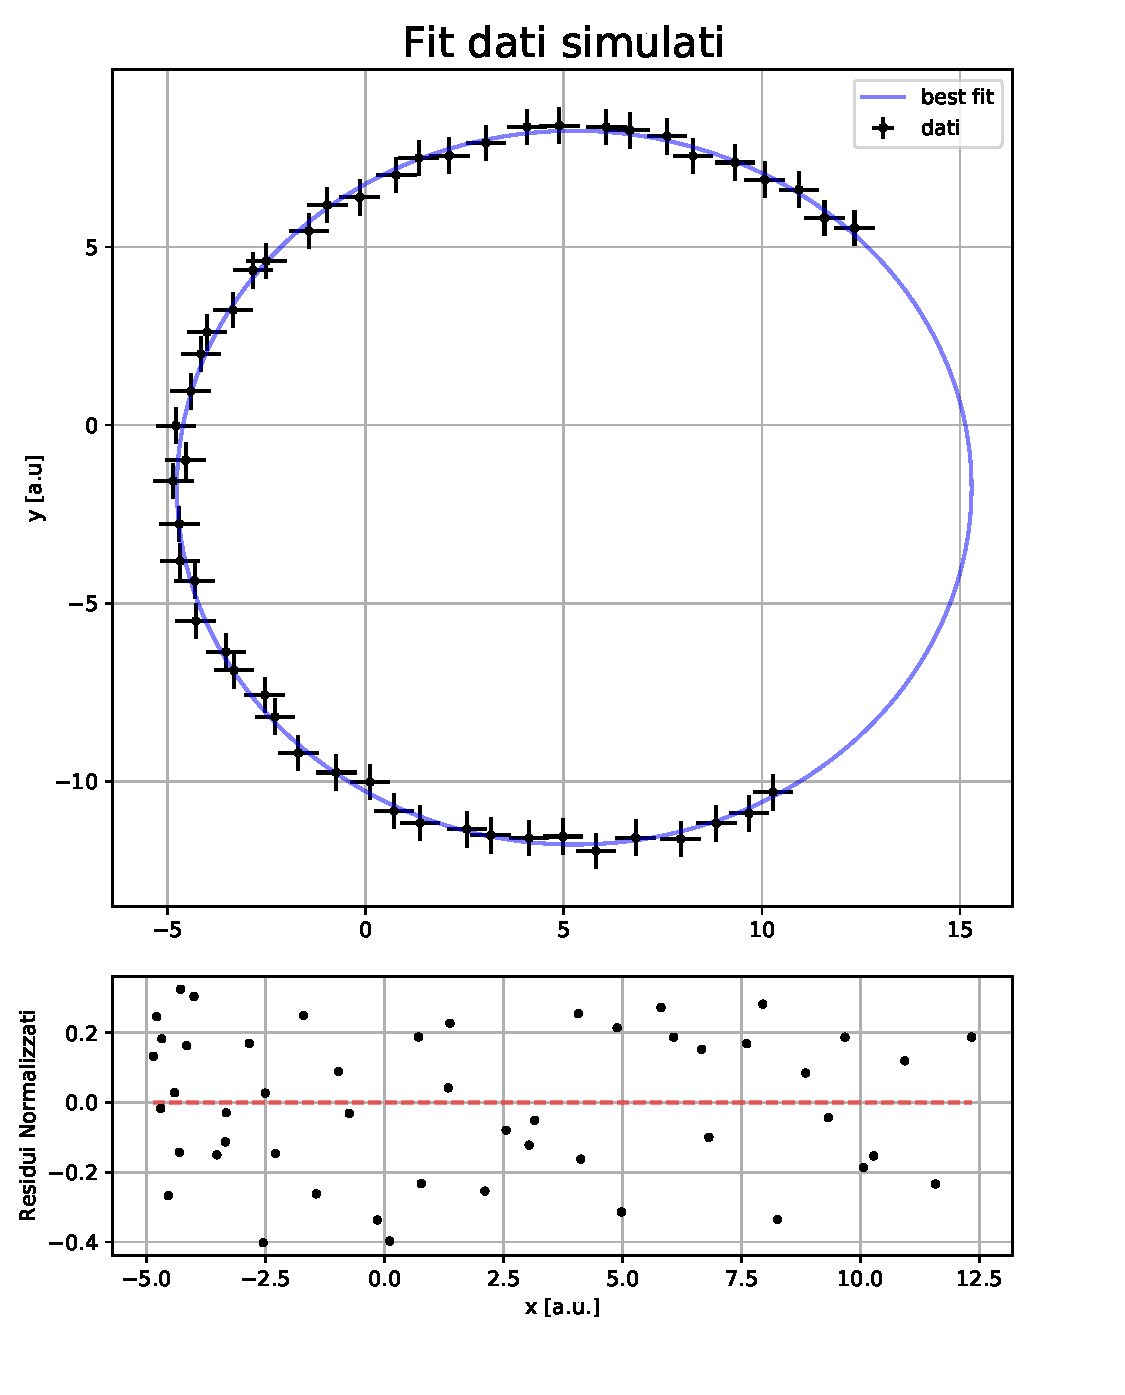
\includegraphics[scale=0.7]{img/fit_cerchio.pdf}
\end{center}



\newpage





\subsection{Fit di un'ellisse, metodo di  Halir e Flusser}
Riportiamo anche un esempio di fit di ellisse basato sull'articolo di Halir e Flusser:  \url{http://autotrace.sourceforge.net/WSCG98.pdf}
(n.d.r. è consigliato leggere l'articolo per i vedere i caveat del metodo).
Non è riportato il calcolo degli errori sui parametri perché nemmeno nell'articolo è trattato.
\begin{lstlisting}[language=Python]
import numpy as np
import matplotlib.pyplot as plt


def ellisse(parametri, n, tmin=0, tmax=2*np.pi):
    """
    Resistuisce un'ellisse di centro (x0, y0),
    di semiassi maggiore e minore (semi_M, semi_m)
    inclinata di un anglo (phi) rispetto all'asse x
    t e' il parametro di "percorrenza" dell'ellisse
    """

    x0, y0, semi_M, semi_m, phi = parametri
    t = np.linspace(tmin, tmax, n)

    x = x0 + semi_M*np.cos(t)*np.cos(phi) - semi_m*np.sin(t)*np.sin(phi)
    y = y0 + semi_M*np.cos(t)*np.sin(phi) + semi_m*np.sin(t)*np.cos(phi)

    return x, y


def cartesiano_a_polari(coef):
    """
    Converte i coefficenti di: ax^2 + bxy + cy^2 + dx + fy + g = 0
    nei coefficeniti polari: centro, semiassi, inclinazione ed eccentricita'
    Per dubbi sulla geometria: https://mathworld.wolfram.com/Ellipse.html
    """
    #i termini misti presentano un 2 nella forma piu' generale
    a = coef[0]
    b = coef[1]/2
    c = coef[2]
    d = coef[3]/2
    f = coef[4]/2
    g = coef[5]

    #Controlliamo sia un ellisse (i.e. il fit sia venuto bene, forse)
    den = b**2 - a*c
    if den > 0:
        Error = 'I coefficenti passati non sono un ellisse: b^2 - 4ac deve essere negativo'
        raise ValueError(Error)

    #Troviamo il centro dell'ellisse
    x0, y0 = (c*d - b*f)/den, (a*f - b*d)/den

    num = 2*(a*f**2 + c*d**2 + g*b**2 - 2*b*d*f - a*c*g)
    fac = np.sqrt((a - c)**2 + 4*b**2)
    #Troviamo i semiassi maggiori e minori
    semi_M = np.sqrt(num/den/(fac - a - c))
    semi_m = np.sqrt(num/den/(-fac - a - c))

    #Controlliamo che il semiasse maggiore sia maggiore
    M_gt_m = True
    if semi_M < semi_m:
        M_gt_m = False
        semi_M, semi_m = semi_m, semi_M

    #Troviamo l'eccentricita'
    r = (semi_m/semi_M)**2
    if r > 1:
        r = 1/r
    e = np.sqrt(1 - r)

    #Troviamo l'angolo di inclinazione del semiasse maggiore dall'asse x
    #l'angolo come solito e misurato in senso antiorario
    if b == 0:
        if a < c :
            phi = 0
        else:
            phi = np.pi/2

    else:
        phi = np.arctan((2*b)/(a - c))/2
        if a > c:
            phi += np.pi/2

    if not M_gt_m :
        phi += np.pi/2

    #periodicita' della rotazione
    phi = phi % np.pi

    return x0, y0, semi_M, semi_m, e, phi


def fit_ellisse(x, y):
    """
    Basato sull'articolo di Halir and Flusser,
    "Numerically stable direct
    least squares fitting of ellipses".
    """

    D1 = np.vstack([x**2, x*y, y**2]).T
    D2 = np.vstack([x, y, np.ones(len(x))]).T

    S1 = D1.T @ D1
    S2 = D1.T @ D2
    S3 = D2.T @ D2

    T = -np.linalg.inv(S3) @ S2.T
    M = S1 + S2 @ T
    C = np.array(((0, 0, 2), (0, -1, 0), (2, 0, 0)), dtype=float)
    M = np.linalg.inv(C) @ M

    eigval, eigvec = np.linalg.eig(M)
    cond = 4*eigvec[0]*eigvec[2] - eigvec[1]**2
    ak = eigvec[:, cond > 0]

    return np.concatenate((ak, T @ ak)).ravel()


if __name__ == "__main__":

    #numero di punti
    N = 100
    #parametri dell'ellissi
    x0, y0 = 4, -3.5
    semi_M, semi_m = 7, 3
    phi = np.pi/4
    #eccentricita' non fondamentale per la creazione
    r = (semi_m/semi_M)**2
    if r > 1:
        r = 1/r
    e = np.sqrt(1 - r)

    #errori
    ex, ey = 0.2, 0.2
    dy = np.array(N*[ey])
    dx = np.array(N*[ex])
    #creiamo l'ellisse
    x, y = ellisse((x0, y0, semi_M, semi_m, phi), N, np.pi/4, 3/2*np.pi)
    k = np.random.uniform(0, ex, N)
    l = np.random.uniform(0, ey, N)
    x = x + k #aggiungo errore
    y = y + l

    coef_cart = fit_ellisse(x, y) #fit

    print('valori esatti:')
    print(f'x0:{x0:.4f}, y0:{y0:.4f}, semi_M:{semi_M:.4f}, semi_m:{semi_m:.4f}, phi:{phi:.4f}, e:{e:.4f}')
    x0, y0, semi_M, semi_m, e, phi = cartesiano_a_polari(coef_cart)
    print('valori fittati')
    print(f'x0:{x0:.4f}, y0:{y0:.4f}, semi_M:{semi_M:.4f}, semi_m:{semi_m:.4f}, phi:{phi:.4f}, e:{e:.4f}')

    #plot
    plt.figure(1)
    plt.title('Fit dati simulati',fontsize=20)
    plt.ylabel('y [a.u]',fontsize=10)
    plt.xlabel('x [a.u]',fontsize=10)
    plt.axis('equal')
    plt.errorbar(x, y, dy, dx, fmt='.', color='black', label='dati')
    x, y = ellisse((x0, y0, semi_M, semi_m, phi), 1000)
    plt.plot(x, y)
    plt.grid()
    plt.show()

[Output]
valori esatti:
x0:4.0000, y0:-3.5000, semi_M:7.0000, semi_m:3.0000, phi:0.7854, e:0.9035
valori fittati
x0:4.0888, y0:-3.4169, semi_M:6.9755, semi_m:2.9975, phi:0.7859, e:0.9030

\end{lstlisting}
\begin{center}
\includegraphics[scale=0.7]{img/fit_ellisse.pdf}
\end{center}





\newpage

\section{Metodi Montecarlo}
In molte simulazioni di interesse fisico è necessario dover generare numeri casuali, o quanto meno pseudo casuali. La generazione di numeri casuali è effettivamente sempre argomento di ricerca per riuscire a raggiungere sempre un livello di casualità maggiore; esistono poi in letteratura esempi di buoni generatori che però in certe simulazioni falliscono, dando risultati fisicamente molto poco sensati. Insomma è un argomento abbastanza delicato. Non potendone parlare nel dettaglio vedremmo brevemente un esempio di generatore di numeri casuali e poi una simulazione vera e propria con l'utilizzo però di librerie di python apposite (sia la libreria numpy che la libreria random, sono molto utili nella generazione di numeri random).

\subsection{Generatori numeri pseudo-casuali}
Uno dei modi più famosi di costruire un generatore è secondo uno schema che ha in nome di: generatore congruenziale lineare. Dato un certo seme $x_0$ posso generare il numero $x_1$ e da questo $x_2$ e via seguendo. Lo schema generale è:
\[
x_{n+1} = (a x_n + c) \mod M
\]
dove $a, c$ e $M$, detti rispettivamente: moltiplicatore, incremento e modulo sono dei numeri scelti con più o meno cura. Vediamo un esempio:

\begin{lstlisting}[language=Python]
import numpy as np

def GEN(r0, n=1, M=2**64, a=6364136223846793005, c=1442695040888963407, norm=True):
    """
    generatore conguenziale lineare
    Parametri
    ---------
    r0 : int
        seed della generazione
    n : int, opzionale
        dimensione lista da generare, di default e' 1
    M : int, opzionale
        periodo del generaltore di default e' 2**64
    a : int, opzionale
        moltiplicatore del generatore, di default e' 6364136223846793005
    c : int, opzionale
        incremento del generatore, di default e' 1442695040888963407
    norm : bool, opzionale
        se True il numero restituito e' fra zero ed 1

    Returns
    ---------
    r : list
        lista con numeri distribuiti casualmente
    """
    if n==1:
        r = (a*r0 + c)%M
    else:
        r = []
        x = r0
        for i in range(1, n):
            x = (a*x + c)%M
            r.append(x)

    if norm :
        if n==1:
            return float(r)/(M-1)
        else :
            return [float(el)/(M-1) for el in r]
    else :
        return r

if __name__ == '__main__':
    seed = 42
    
    print(GEN(seed, n=5))
    momenti1 = [np.mean(np.array(GEN(seed, n=int(5e5)))**i) for i in range(1, 10)]
    momenti2 = [1/(1+p) for p in range(1, 10)]
    
    for M1, M2 in zip(momenti1, momenti2):
        print(f'{M1:.3f}, {M2:.3f}')

[Output]
[0.5682303266439077, 0.22546342894775137, 0.41283831882951183, 0.6303980498395979]
0.500, 0.500
0.333, 0.333
0.250, 0.250
0.200, 0.200
0.167, 0.167
0.143, 0.143
0.125, 0.125
0.111, 0.111
0.100, 0.100
\end{lstlisting}
Quello che si fa a Riga 47 è il calcolo dei primi momenti della distribuzione uniforme con il nostro generatore; alla riga successiva troviamo i momenti analitici, da confrontare con quelli da noi calcolati per fare un piccolo test sulla bontà del generatore.

\subsection{Calcolo di Pi greco}
Prendete dei coriandoli e buttateli a caso su una mattonella con un cerchio disegnato sopra e contando quanti sono dentro al cerchio rispetto al totale avete calcolato $\pi$.
Fondamentalmente quel che si fa è il calcolo di un'area (i.e. un'integrale) e benché ci siano modi più efficienti il calcolo di $\pi$ è un classico esempio e quindi non mancheremo di esporlo. La particolarità di usare un metodo Monte-Carlo infatti si vede in alte dimensioni poiché a differenza dei possibili metodi di integrazione che uno può inventarsi l'errore dato da Monte-Carlo non dipende dalla dimensione ma va sempre come $1/\sqrt{N}$. Per comodità l'esempio è fatto su un quarto di circonferenza quindi la probabilità che il coriandolo sia dentro è $\pi/4$.

\begin{lstlisting}[language=Python]
import time
import numpy as np
import matplotlib.pyplot as plt

N = int(5e4)
start_time=time.time()

x = np.linspace(0,1, 10000)

def f(x):
    """
    semi circonferenza superiore
    """
    return np.sqrt(1-x**2)

c     = 0
X_in  = []
Y_in  = []
X_out = []
Y_out = []

for i in range(1,N):
    #genero due variabili casuali uniformi fra 0 e 1
    a = np.random.rand()
    b = np.random.rand()
    r = a**2 + b**2
    #se vero aggiorno c di 1
    if r < 1:
        X_in.append(a)
        Y_in.append(b)
        c += 1
    else:
        X_out.append(a)
        Y_out.append(b)

#moltiplico per quattro essendo su un solo quadrante
Pi = 4*c/N
#propagazione errore, viene dalla binomiale
dPi = np.sqrt(c/N * (1-c/N))/np.sqrt(N)
print('%f +- %f' %(Pi, dPi))
print(np.pi)
print(abs((Pi-np.pi)/np.pi))

plt.figure(1)
plt.title('Pi $\simeq$ %.3f $\pm$ %.3f ; N=%.0e' %(Pi, dPi, N), fontsize=20)
plt.xlim(0,1)
plt.ylim(0,1)
plt.plot(x, f(x),color='blue', lw=1)
plt.errorbar(X_in, Y_in,   fmt='.', markersize=1, color='blue')
plt.errorbar(X_out, Y_out, fmt='.', markersize=1,  color='green')
ax  = plt.gca()
ax.set_aspect('equal')
plt.show()

print("--- %s seconds ---" % (time.time() - start_time))

[Output]
3.142720 +- 0.001835
3.141592653589793
0.0003588455075227156
--- 0.19469761848449707 seconds ---
\end{lstlisting}

Cambiando N si può controllare quanto velocemente questo metodo converga, e si vedrà che non è velocissimo ma va beh, come dicevamo prima siamo solo in due dimensioni.

\begin{center}
\includegraphics[scale=0.9]{img/mont_pi.png}
\end{center}
(ok, sgrana un po' ma in pdf era troppo pesante e il pdf non scorreva bene)

\newpage

\section{Propagazione errori}
Può capitare spesso che vadano propagati degli errori, purtroppo. A Laboratorio 1 si vede che il modo di propagarli è fare le derivate, e in casi più semplici ci sono dei trucchetti. Noi per andare sul sicuro faremo sempre le derivate, dove il guaio è che è facile sbagliare i calcoli, ma per fortuna noi li facciamo fare al computer.

\subsection{Propagarli a mano}
Volendo scrivere un breve codice facile da modificare all'occorrenza si potrebbe provare così:
\begin{lstlisting}[language=Python]
import numpy as np
import sympy as sp

x = sp.Symbol('x')
y = sp.Symbol('y')
z = sp.Symbol('z')
t = sp.Symbol('t')

def Errore(x1, dx1, y1, dy1, z1, dz1, t1, dt1):
    """
    Prende in input certe quantita' con un errore
    e propaga l'errore su una certa funzione di queste
    """
    #funzione su cui propagare l'errore da modifica all'occorenza
    f1 = ((x-y)/(z+t))

    #valor medio
    f = float(f1.subs(x,x1).subs(y,y1).subs(z,z1).subs(t,t1))

    #derivate parziali calcolate nel punto
    a = sp.diff(f1, x).subs(x,x1).subs(y,y1).subs(z,z1).subs(t,t1)
    b = sp.diff(f1, y).subs(x,x1).subs(y,y1).subs(z,z1).subs(t,t1)
    c = sp.diff(f1, z).subs(x,x1).subs(y,y1).subs(z,z1).subs(t,t1)
    d = sp.diff(f1, t).subs(x,x1).subs(y,y1).subs(z,z1).subs(t,t1)

    #somma dei vari contributi
    df1 = ((a*dx1)**2 + (b*dy1)**2+ (c*dz1)**2 + (d*dt1)**2 )
    df = np.sqrt(float(df1))

    return f, df


print(Errore(1, 0.1, 2, 0.1, 3, 0.1, 2, 0.1))

[Output]
(-0.2, 0.02884441020371192)
\end{lstlisting}

\subsection{Uncertainties}
Oppure volendo si potrebbe usare questa comoda libreria:

\begin{lstlisting}[language=Python]
from uncertainties import ufloat
import uncertainties.umath as um

#il pimo argomento e' il valore centrale, il secondo l'errore
x = ufloat(7.1, 0.2)
y = ufloat(12.3, 0.7)


print(x)
print(2*x-y)
print(um.log(x**y))

[Output]
7.10+/-0.20
1.9+/-0.8
24.1+/-1.4
\end{lstlisting}

Vediamo ora un riassunto della propagazione degli errori:

\includegraphics[scale=1.5]{img/analisi.jpeg}



\newpage

\section{Interpolazione}
Nel mondo della fisica computazionale, ad esempio nel mondo dell'astrofisica computazionale, capita spesso che alcune cose siano tabulate. Ovvero per fare una qualche simulazione si prendono delle certe quantità a loro volta frutto in genere di simulazioni e che quindi sono date per passi; se però fossimo interessati ad analizzare determinati valori magari in un range con un passo più piccolo della tabella, dobbiamo necessariamente interpolare, per cercare di capire cosa succede tra i due punti nella tabella.
\subsection{Interpolazione lineare}
Il modo più semplice è unire i punti con una retta, ovvero eseguire un'interpolazione lineare. Dati due punti consecutivi nella tabella indicati come $(x_i, y_i)$ e $(x_{i+1}, y_{i+1})$ l'interpolazione lineare non fa altro che assegnare ad ogni valore di $x$  compreso nell'intervallo $[x_i, x_{i+1}]$ la media ponderata tra $y_i$  e $y_{i+1}$.
\[
f(x) = \frac{x_{i+1} - x}{x_{i+1} - x_{i}} y_i + \frac{x-x_{i}}{x_{i+1}- x_{i}} y_{i+1}
\]
L'espressione precedente non è altro quindi che la retta che unisce i due punti. Vediamo il codice:

\begin{lstlisting}[language=Python]
import numpy as np
import matplotlib.pyplot as plt

def f(x, xx, yy):
    """
    restituisce l'interpolazione dei punti xx yy
    x puo' essere un singolo valore in cui calcolare
    la funzione interpolante o un intero array
    """
    #proviamo se x e' un array
    try :
        n = len(x)
        x_in = np.min(xx) <= np.min(x) and np.max(xx) >= np.max(x)
    except TypeError:
        n = 1
        x_in = np.min(xx) <= x <= np.max(xx)

    #se il valore non e' nel range corretto e' impossibile fare il conto
    if not x_in :
        a = 'uno o diversi valori in cui calcolare la funzione'
        b = ' interpolante sono fuori dal range di interpolazione'
        errore = a+b
        raise Exception(errore)

    #array che conterra' l'interpolazione
    F = np.zeros(n)

    if n == 1 :
        #controllo dove e' la x e trovo l'indice dell'array
        #per sapere in che range bisogna interpolare
        for j in range(len(xx)-1):
            if xx[j] <= x <= xx[j+1]:
                i = j

        A = yy[i] * (xx[i+1] - x)/(xx[i+1] - xx[i])
        B = yy[i+1] * (x - xx[i])/(xx[i+1] - xx[i])
        F[0] = A + B

    else:
        #per ogni valore dell'array in cui voglio calcolare l'interpolazione
        for k, x in enumerate(x):
            #controllo dove e' la x e trovo l'indice dell'array
            #per sapere in che range bisogna interpolare
            for j in range(len(xx)-1):
                if xx[j] <= x <= xx[j+1]:
                    i = j

            A = yy[i] * (xx[i+1] - x)/(xx[i+1] - xx[i])
            B = yy[i+1] * (x - xx[i])/(xx[i+1] - xx[i])
            F[k] = A + B

    return F

if __name__ == '__main__':
    x = np.linspace(0, 1, 10)
    y = np.sin(2*np.pi*x)
    z = np.linspace(0, 1, 100)

    plt.figure(1)
    plt.title('Interpolazione lineare')
    plt.xlabel('x')
    plt.ylabel('y')
    plt.plot(z, f(z, x, y), 'b', label='interpolazione')
    plt.plot(x, y, marker='.', linestyle='', c='k', label='dati')
    plt.legend(loc='best')
    plt.grid()
    plt.show()
\end{lstlisting}

La funzione scritta prende due array "xx" e "yy" che sono i dati da interpolare, e una variabile "x" che può essere un singolo punto dell'intervallo o un intero array per ottenere una curva. Si è usato un try except perché chiaramente Python da errore se si calcola la lunghezza di un numero. Vi è poi il sollevamento di un'eccezione in caso i valori di interesse siano fuori dagli estremi della tabella dove non si può dire nulla quindi il codice si interrompe. Vediamo il risultato:

\begin{center}
\includegraphics[scale=0.8]{img/int_lin.pdf}    
\end{center}

\subsection{Interpolazione Polinomiale}
Un altro modo per interpolare è usare un polinomio di grado $n-1$ per $n$ punti e si può fare facilmente con la matrice di Vandermonde, il problema è che tale matrice è mal condizionata, quindi non funziona sempre benissimo e il costo computazionale è alto dato che bisogna invertire una matrice.

\[
\begin{bmatrix}
1 & x_1 & x_1^2 & \dots & x_1^{n-1}\\
1 & x_2 & x_2^2 & \dots & x_2^{n-1}\\
1 & x_3 & x_3^2 & \dots & x_3^{n-1}\\
\vdots & \vdots & \vdots & \ddots &\vdots \\
1 & x_m & x_m^2 & \dots & x_m^{n-1}
\end{bmatrix}
\hspace{1.5 mm}
\begin{bmatrix}
  s_0 & \\
  s_1 & \\
  s_2 & \\
  \vdots & \\
  s_{n-1} &
\end{bmatrix}
\hspace{1.5 mm} = \hspace{1.5 mm}
\begin{bmatrix}
  y_1 & \\
  y_2 & \\
  y_3 & \\
  \vdots & \\
  y_m &
\end{bmatrix}
\]
Dove le $x$ e le $y$ sono i nostri dati tabulati e gli $s_i$ sono i coefficienti del polinomio. Vediamo un semplice esempio di codice:

\begin{lstlisting}[language=Python]
import numpy as np
import matplotlib.pyplot as plt

N = 10
x = np.linspace(0, 1, N)
y = np.sin(2*np.pi*x)

#Matrice di Vandermonde
A = np.zeros((N, N))
A[:,0] = 1
for i in range(1, N):
    A[:,i] = x**i

#risolvo il sistema, la soluzione sono i coefficenti del polinomio
s = np.linalg.solve(A, y)


def f(s, zz):
    '''
    funzione per fare il grafico
    '''
    n = len(zz)
    y = np.zeros(n)
    for i , z in enumerate(zz):
        y[i] = sum([s[j]*z**j for j in range(len(s))])
    return y

z = np.linspace(0, 1, 100)

plt.figure(1)
plt.title('Interpolazione polinomiale')
plt.xlabel('x')
plt.ylabel('y')
plt.plot(z, f(s, z), 'b', label='interpolazione')
plt.plot(x, y, marker='.', linestyle='', c='k', label='dati')
plt.legend(loc='best')
plt.grid()
plt.show()
\end{lstlisting}

\begin{center}
\includegraphics[scale=0.8]{img/int_pol.pdf}    
\end{center}

\subsection{Scipy.interpolate}
Ovviamente esiste una libreria di Python che ci permette facilmente di eseguire le interpolazioni, riportiamo un semplice esempio (ricordando sempre che il modo migliore per capire a pieno è leggere la documentazione).


\begin{lstlisting}[language=Python]
import numpy as np
import matplotlib.pyplot as plt
from scipy.interpolate import InterpolatedUnivariateSpline

N = 10
x = np.linspace(0, 1, N)
y = np.sin(2*np.pi*x)

#interpolazione con una, spline cucbica (k=3)
s3 = InterpolatedUnivariateSpline(x, y, k=3)

z = np.linspace(0, 1, 100)

plt.figure(1)
plt.title('Interpolazione spline cubica')
plt.xlabel('x')
plt.ylabel('y')
plt.plot(z, s3(z), 'b', label='interpolazione')
plt.plot(x, y, marker='.', linestyle='', c='k', label='dati')
plt.legend(loc='best')
plt.grid()
plt.show()
\end{lstlisting}

\begin{center}
\includegraphics[scale=0.8]{img/int_spline.pdf}    
\end{center}


\newpage

\section{Risolve numericamente le SDE}
Nelle sezioni precedenti abbiamo parlato delle equazioni differenziali alle derivate ordinarie (ODE) e alle derivate parziali (PDE); veniamo ora a fare un piccolo accenno alle equazioni differenziali stocastiche (SDE). Le SDE sono equazioni in cui un termine è un processo stocastico e quindi anche la soluzione sarà un processo stocastico; sono utilizzate per modellare gli andamenti dei mercati o un qualche fenomeno soggetto a fluttuazioni termiche. Vedremo due semplici esempi, il moto geometrico Browniano e un processo di Ornstein–Uhlenbeck.

\subsection{Processo di Ornstein–Uhlenbeck}
Un processo di Ornstein–Uhlenbeck è descritto dalla seguente equazione stocastica:
\[
dx = \theta (\mu -  x) \, dt + \sigma \, dW
\]
dove $ \theta, \sigma$ constanti positive e $\mu$ costante, mentre $dW$ è un processo di Wiener. In genere data una certa SDE della forma:
\[
dx = f(x) dt + g(x) dW,
\]
possiamo risolverla nel seguente modo (metodo di Euler–Maruyama):

\[
x_{n+1} = x_n + f(x_n) dt + g(x_n) dW
\]
dove $dt$ ora è il passo di integrazione e $dW$, che sarebbe un integrale stocastico, lo trattiamo una variabile gaussiana di media zero e varianza uguale alla radice del passo di integrazione. Vediamo un semplice esempio:

\begin{lstlisting}[language=Python]
import numpy as np
import matplotlib.pyplot as plt

def f(z):
    """
    funzione che moltiplica il dt
    """
    theta = 0.7
    mu = 2.5
    return theta * (mu - z)

def g():
    """
    funzione che moltimplica il processo di wiener
    """
    sigma = 0.6
    return sigma

def dW(delta_t):
    """
    processo di wiener trattato come variabile gaussiana
    """
    return np.random.normal(loc=0.0, scale=np.sqrt(delta_t))

#parametri simulazione
N = 10000
tf = 15
dt = tf/N

ts = np.zeros(N + 1)
ys = np.zeros(N + 1)
xs = np.zeros(N + 1)

ys[0], xs[0] = 0, 0 #condizioni inizali

for i in range(N):
    ys[i+1] = ys[i] + f(ys[i]) * dt + g() * dW(dt)
    xs[i+1] = xs[i] + f(xs[i]) * dt + g() * dW(dt)
    ts[i+1] = ts[i] + dt

plt.figure(1)
plt.plot(xs, ys)
plt.title('Ornstein Uhlenbeck')
plt.xlabel("x")
plt.ylabel("y")
plt.grid()

plt.figure(2)
plt.plot(ts, xs, label='x(t)')
plt.plot(ts, ys, label='y(t)')
plt.title('Ornstein Uhlenbeck')
plt.xlabel("t")
plt.legend()
plt.grid()

plt.show()
\end{lstlisting}

\begin{multicols}{2}


\includegraphics[scale=0.55]{img/OU_1.pdf}


\includegraphics[scale=0.55]{img/OU_2.pdf}


\end{multicols}

\subsection{Moto geometrico Browniano}
Il moto geometrico browniano è un moto browniano esponenziale, che ha applicazioni nella descrizione dei mercati finanziari ad esempio; l'equazione associata è:
\[
dx = \mu x dt + \sigma x dW
\]
Vedremo per risolverla il metodo di heun che si può scrivere così, facendo riferimento all'equazione generica di sopra($dx = f(x) dt + g(x) dW$):
\[
\begin{cases}
\overline{x} = x_n + z_1 g(x_n) + f(x_n) dt + \frac{1}{2} g(x_n)g^{'}(x_n) z_1^2 \\
\hat{x} = x_n + z_1 g(\overline{x}) + f(\overline{x}) dt + \frac{1}{2} g(\overline{x})g^{'}(\overline{x}) z_1^2 \\
x_{n+1} = \frac{1}{2}( \hat{x} + \overline{x} )
\end{cases}
\]
dove $z_1$ rappresenta il processo di wiener ed è sempre una variabile gaussiana a media zero e varianza $dt$. Vediamone l'implementazione:

\begin{lstlisting}[language=Python]
import numpy as np
import matplotlib.pyplot as plt

# geometric Brownian motion
# Heun method

def f(z):
    """
    funzione che moltiplica il dt
    """
    mu = 1
    return mu*z

def g(z):
    """
    funzione che moltimplica il processo di wiener
    """
    sigma = 0.5
    return sigma*z

def dg():
    """
    derivata di g
    """
    sigma = 0.5
    return sigma

def dW(delta_t):
    """
    processo di wiener trattato come variabile gaussiana
    """
    return np.random.normal(loc=0.0, scale=np.sqrt(delta_t))


#parametri simulazioni
N = 10000
tf = 4
dt = tf/N
#faccio 5 simulazioni diverse
for _ in range(5):
    #array dove conservare la soluzione, ogni volta inizializzati
    ts = np.zeros(N + 1)
    ys = np.zeros(N + 1)

    ys[0] = 1#condizioni iniziali

    for i in range(N):
        ts[i+1] = ts[i] + dt
        y0 = ys[i] + f(ys[i])*dt + g(ys[i])*dW(dt) + 0.5*g(ys[i])*dg()*(dW(dt)**2)
        y1 = ys[i] + f(y0)*dt    + g(y0)*dW(dt)    + 0.5*g(y0)*dg()*(dW(dt)**2)
        ys[i+1] = 0.5*(y0 + y1)

    plt.plot(ts, ys)

plt.figure(1)
plt.title('moto geometrico Browniano')
plt.xlabel("time")
plt.grid()

plt.show()

\end{lstlisting}

\begin{center}
\includegraphics[scale=0.75]{img/gmb.pdf}    
\end{center}

\newpage

\section{Ottimizzazione}
Per quanto la discussione fatta nella quarta lezione con curve\_fit sia appunto di ottimizzazione, parliamo brevemente degli algoritmi di ottimizzazione. Tratteremo del gradiente discendente e di una sua modifica spiegando al computer che esiste il principio di inerzia.
Sia $F(x): \mathbb{R}^n \rightarrow \mathbb{R}$ la funzione da minimizzare. 
\subsection{Discesa del gradiente}
La regola del gradiente discendente ci fa aggiornare iterativamente il punto di minimo con:
\begin{equation}
x_{n+1} = x_n - \alpha_n \nabla F(x_n)
\end{equation}
Ci sono vari modi per scegliere $\alpha_n$ noi lo supporremo costante, scelta non delle migliori, perché può allungare la convergenza del metodo. Ricordiamo inoltre che i metodi iterativi convergono solo a minimi locali quindi bisogna scegliere attentamente il punto iniziale.
\begin{lstlisting}[language=Python]
def grad_disc(f, x0, tol, step):
    """
    implementation of gradient descent
    you have to be careful about the values
    you pass in x0 if the function has more minima
    and also the value of steps is a delicate choice
    to be made wisely

    Parameters
    ----------
    f : callable
        function to find the minimum,
        can be f(x), f(x,y) and so on
    x0 : 1darray
        initial guess, to choose carefully
    tol : float
        required tollerance
        the function stops when all components
        of the gradient have smaller than tol
    step : float
        size of step to do, to choose carefully

    Returns
    -------
    X : ndarray
        array with all steps of solution
    iter : int
        number of iteration
    """
    iter = 0               #initialize iteration counter
    h = 1e-7               #increment for derivatives
    X = []                 #to store solution
    M = len(x0)            #number of variable
    s = np.zeros(M)        #auxiliary array for derivatives
    grad = np.zeros(M)     #gradient

    while True:
        #gradient computation
        for i in range(M):                       #loop over variables
            s[i] = 1                             #we select one variable at a time
            dz1 = x0 + s*h                       #step forward
            dz2 = x0 - s*h                       #step backward
            grad[i] = (f(*dz1) - f(*dz2))/(2*h)  #derivative along z's direction
            s[:] = 0                             #reset to select the other variables

        if all(abs(grad) < tol):
            break

        x0 = x0 - step*grad   #move towards the minimum
        X.append(x0)          #store iteration
        iter += 1             #update counter

    X = np.array(X)
    return X, iter
\end{lstlisting}

\subsection{Principio di inerzia}
Fondamentalmente se vediamo l'evoluzione della soluzione è come se una pallina stesse scendendo lungo una verde vallata, cioè la nostra $F$ è il potenziale a cui la pallina è soggetta, quindi in analogia con la fisica si introduce il : gradiente discendente con momento. Cioè sia ggiunge un termine di velocità e un termine di attrito dipendente dalla velocità in modo che l'algoritmo non oscilli.
\begin{align}
w_{n+1} &= \beta w_n + \nabla F(x_n) \\
x_{n+1} &= x_n - \alpha w_{n+1}
\end{align}
$\alpha$ è sempre lo step mentre $\beta$ rappresenta pittoricamente il coefficiente di attrito. Se $\beta=1$ l'algoritmo oscilla tra due punti con lo stesso valore di $F$ (si conserva l'energia) quindi bisogna avere $\beta<1$.
\begin{lstlisting}[language=Python]
def grad_disc_m(f, x0, tol, alpha, beta):
    """
    implementation of gradient descent with momentum
    you have to be careful about the values
    you pass in x0 if the function has more minima
    and also the value of alpha an beta is a
    delicate choice to be made wisely

    Parameters
    ----------
    f : callable
        function to find the minimum,
        can be f(x), f(x,y) and so on
    x0 : 1darray
        initial guess, to choose carefully
    tol : float
        required tollerance
        the function stops when all components
        of the gradient have smaller than tol
    alpha : float
        size of step to do, to choose carefully
    beta : float
        size of step to do for velocity,
        to choose carefully, if beta = 0
        we get the method of gradient
        descent without momentum

    Returns
    -------
    X : ndarray
        array with all steps of solution
    iter : int
        number of iteration
    """
    iter = 0               #initialize iteration counter
    h = 1e-7               #increment for derivatives
    X = []                 #to store solution
    M = len(x0)            #number of variable
    s = np.zeros(M)        #auxiliary array for derivatives
    grad = np.zeros(M)     #gradient
    w = np.zeros(M)        #velocity, momentum

    while True:
        #gradient computation
        for i in range(M):                       #loop over variables
            s[i] = 1                             #we select one variable at a time
            dz1 = x0 + s*h                       #step forward
            dz2 = x0 - s*h                       #step backward
            grad[i] = (f(*dz1) - f(*dz2))/(2*h)  #derivative along z's direction
            s[:] = 0                             #reset to select the other variables

        if all(abs(grad) < tol):
            break

        w = beta*w + grad     #update velocity
        x0 = x0 - alpha*w     #update position move towards the minimum
        X.append(x0)          #store iteration
        iter += 1             #update counter

    X = np.array(X)
    return X, iter
\end{lstlisting}

Vediamo ora due grafici per capire il risultato, non mostriamo il codice in quanto si tratta semplicemente di chiamare le funzioni e fare i plot.


\begin{center}
\includegraphics[scale=0.75]{img/minimo1d.pdf}
\end{center}


Le funzioni sono state chiamate con i parametri $grad\_disc(G, x0, 1e-8, 1e-3)$ e $grad\_disc\_m(G, x0, 1e-8, 1e-3, 0.953)$ la funzione da minimizzare è $F(x)=(x^2 - 1)^2 + x$ vediamo che il primo data una infelice scelta del punto di partenza si incastra in un minimo locale. Il secondo invece arriva al minimo locale con un valore della velocità non nullo e quindi riesce a scavalcare il massimo locale se $\beta$ fosse stato $0.9$ anche lui si sarebbe bloccato lì. Le curve sono state traslate per maggiore leggibilità. Con gli stessi parametri vediamo un esempio bidimensionale (il codice è lo stesso la funzione è implementata in modo generico). $F(x, y) = (x^2 + y - 11)^2 + (x + y^2 - 7)^2$.


\begin{center}
\includegraphics[scale=0.9]{img/minimo2d.pdf}
\end{center}




\newpage

\section{Machine Learning}
Nell'ultima lezione del corso avanzato abbiamo visto una breve introduzioni alle rete neurali. Ora vogliamo sempre parlare di machine learning ma usando la libreria 'sklearn'. Vediamo quindi un esempio che possa essere il corrispettivo di un "Hello World". Ci limiteremo, come sopra, al machine learning supervisionato ovvero sappiamo sia input che output. Mostreremo un esempio di classificatore e uno di regressore.

\subsection{Classificatore}
Un algoritmo classificatore fondamentalmente prende dei dati e restituisce una categoria, quindi classifica i dati in input. Vediamo un esempio:

\begin{lstlisting}[language=Python]
import scikitplot as skplt
import matplotlib.pyplot as plt
from sklearn import datasets
from sklearn.model_selection import train_test_split
from sklearn.tree import DecisionTreeClassifier
from sklearn.metrics import accuracy_score

#dati che verrano utilizzati
iris_dataset = datasets.load_iris()
#print(iris_dataset["DESCR"])

#caratteristiche, dati in input
x = iris_dataset.data

#output, cioe' quello che il modello dovrebbe predire
y = iris_dataset.target

#divido i dati, un parte li uso per addestrare, l'altra per
#testare se il modello ha imparato bene
x_train, x_test, y_train, y_test = train_test_split(x, y)

#modello non addestrato, classificatore
#un classificatore prende i dati e restituisce un categoria
modello = DecisionTreeClassifier()

#addestro il modello
modello.fit(x_train, y_train)

#predizioni sui dati su cui ha imparato
predizione_train = modello.predict(x_train)

#predizioni su nuovoi dati
predizione_test = modello.predict(x_test)

#misuro l'accuratezza sia dell'addestramento che del test
#questo puo' dare informazioni su over fitting o meno
#sinceramente non so come
print("accuratezza train")
print(accuracy_score(y_train, predizione_train))

print("accuratezza test")
print(accuracy_score(y_test, predizione_test))

#Rappresentazione grafica dei quanto e' stato bravo il modello
#sulle y c'e' la risposta che il modello doveva dare e
#sulle x ci sta la predizione che il modello ha dato, quindi gli
#elementi fuori diagonali sono le risposte sbagliate
skplt.metrics.plot_confusion_matrix(y_train,predizione_train)
skplt.metrics.plot_confusion_matrix(y_test,predizione_test)

plt.show()

[Output]
accuratezza train
1.0
accuratezza test
0.9736842105263158

\end{lstlisting}

\begin{multicols}{2}


\includegraphics[scale=0.5]{img/clas_conf_mat_train.png}


\includegraphics[scale=0.5]{img/clas_conf_mat_test.png}


\end{multicols}
La matrice di sinistra ci fa vedere come la predizione sui dati che abbiamo usato per addestrarla sia andata bene, infatti avevamo accuratezza uno; a sinistra vediamo che il modello ha dato una sola risposta sbagliata sui dati di test.

\subsection{Regressori}
Un regressore prende dei dati e restituisce un numero; è un po' come quando si fa un fit, circa...

\begin{lstlisting}[language=Python]
import numpy as np
from sklearn.datasets import load_boston
from sklearn.linear_model import LinearRegression
from sklearn.metrics import mean_absolute_error
from sklearn.model_selection import train_test_split

"""
utilizzo di un regressore lineare per predirre
Il prrezzo di una casa dati certe informazioni
"""
dataset = load_boston()

#print(dataset["DESCR"])
#primi 13 elemnti della prima riga
#print(dataset["data"][0])
#ultimo elemnto della prima riga
#print(dataset["target"][0])

#caratteristiche
X = dataset["data"]

#output, cioe' quello che il modello dovrebbe predire
y = dataset["target"]

#divido i dati, un parte li uso per addestrare, l'altra per
#testare se il modello ha imparato bene
X_train, X_test, y_train, y_test = train_test_split(X, y)

#modello non addrestato e' un regressore
#un regressore prende i dati e restituisce un numero, una stima di qualcosa
modello = LinearRegression()

#addestro il modello
modello.fit(X_train, y_train)

#predizioni
p_train = modello.predict(X_train)
p_test = modello.predict(X_test)

#errori sulla predizione
dp_train = mean_absolute_error(y_train, p_train)
dp_test = mean_absolute_error(y_test, p_test)

print("train", np.mean(y_train),"+-", dp_train)
print("test ", np.mean(y_test), "+-", dp_test)

[Output]
train 22.59815303430079 +- 3.1207001914064647
test  22.337795275590548 +- 3.806645940024761
\end{lstlisting}

\subsection{Salvare il modello}

Ora giustamente voi mi potreste obbiettare: Sì tutto molto bello, ma se spengo il computer il modello muore e devo riaddestrarlo. Effettivamente avete ragione ma chiaramente ci sta una soluzione a tutto ciò, nessuno vuole perdere tempo a riaddestrare il modello ogni volta che accende il pc. Vedremo due comandi della libreria 'joblib' che ci permetteranno di salvare il modello e di caricarlo poi su un altro codice. Per fare un semplice esempio che possa scalare bene con i parametri, consideriamo un classificatore a cui diamo in input una matrice $N \times M$ contenete delle curve del tipo $y(x) = x^k$ dove $k \in [0, 1]$. Prendiamo per k ad esempio $5$ valori, e calcoliamo $M$ curve in totale ognuna lunga $N$. Per rendere le cose un po' più complicate per la macchina il range in cui calcolare le curve è scelto a caso. Vediamo ora il codice:

\begin{lstlisting}[language=Python]
'''
code that trains a model and saves it
'''
import joblib
import numpy as np
import scikitplot as skplt
import matplotlib.pyplot as plt
from sklearn.metrics import accuracy_score
from sklearn.tree import DecisionTreeClassifier
from sklearn.model_selection import train_test_split

path = r'C:\Users\franc\desktop\mod.sav'

#=========================================================
# Creation of data set
#=========================================================

M = 30000 # numer data
N = 200   # len of each curve

X = np.zeros((N, M))          # matrix of featurs
d = np.linspace(0, 1, 5)      # parameter of curvese
t = np.zeros(M)               # target index of d

for i in range(M):

    # random interval
    x1, x2 = np.random.random(2)*5
    # each features is nothing but a curve y=x**k with k element of d
    k = d[i%len(d)]
    X[:, i] = np.linspace(x1, x2, N)**k
    # the target must be integer so we use the corrispective indices
    t[i] = i%len(d)

#=========================================================
# Creation and training of model
#=========================================================

x = X.T
y = t
# split fro train ad test
x_train, x_test, y_train, y_test = train_test_split(x, y)

# define the model
modello = DecisionTreeClassifier()
# I train the model
modello.fit(x_train, y_train)
# predictions about the data on which it has learned
prediction_train = modello.predict(x_train)
# prediction on new data
prediction_test  = modello.predict(x_test)

# accuracy
print("accuracy train")
print(accuracy_score(y_train, prediction_train))

print("accuracy test")
print(accuracy_score(y_test, prediction_test))

#=========================================================
# Plot confusion matrix
#=========================================================

skplt.metrics.plot_confusion_matrix(y_train, prediction_train)
skplt.metrics.plot_confusion_matrix(y_test,  prediction_test)

plt.show()

#=========================================================
# Save model
#=========================================================

joblib.dump(modello, path)

[Output]
accuracy train
1.0
accuracy test
0.8012
\end{lstlisting}

\begin{multicols}{2}


\includegraphics[scale=0.5]{img/pred_know_data.png}


\includegraphics[scale=0.5]{img/pred_data.png}


\end{multicols}
Per rendere fattibile la cosa il target non è il valore dell'esponente ma l'indice dell'array in cui il valore è contenuto. Ora che abbiamo salvato il modello, possiamo spegnere il computer e se ci capita per strada un set di dati per cui la nostra macchina è stata addestrata possiamo riusarlo. Vediamo come si fa:

\begin{lstlisting}[language=Python]
'''
code that takes a model saved on your computer and uses it to make predictions
'''
import joblib
import numpy as np
import scikitplot as skplt
import matplotlib.pyplot as plt
from sklearn.metrics import accuracy_score

modello = joblib.load(r'C:\users\franc\desktop\mod.sav')

#=========================================================
# Creation of data set with same features
#=========================================================

M = 1000 # numer data
N = 200 # len of each curve

X = np.zeros((N, M))          # matrix of featurs
d = np.linspace(0, 1, 5)      # parameter of curvese
t = np.zeros(M)               # target index of d

for i in range(M):

    # random interval
    x1, x2 = np.random.random(2)*5
    # each features is nothing but a curve y=x**k with k element of d
    k = np.random.choice(d)
    X[:, i] = np.linspace(x1, x2, N)**k
    # the target must be integer so we use the corrispective indices
    t[i] = np.where(k==d)[0][0]

#=========================================================
# Prediction on new data
#=========================================================

prediction = modello.predict(X.T)

print(f'Accuracy score = {accuracy_score(t, prediction)}')

skplt.metrics.plot_confusion_matrix(t, prediction)

plt.show()

[Output]
Accuracy score = 0.785

\end{lstlisting}
Vediamo che l'accuratezza e abbastanza buona, parente di quella sui dati di test del precedente codice. Qui il parametro che possiamo settare in maniera diversa è $M$, se proviamo a cambiane $N$ otterremmo un errore, perché chiaramente la macchina sa fare solo quello per cui è stata addestrata.

\begin{center}
\includegraphics[scale=0.7]{img/pred_mod_loc.png}
\end{center}

\newpage


\section{Creare un eseguibile}

Abbiamo visto che Python è un linguaggio interpretato e non compilato quindi non viene creato un eseguibile. Supponiamo però vi venga in mente di creare un eseguibile, come facciamo?
Ci serve un pacchetto: pyinstaller, che ci permette di creare un eseguibile, con il caveat che se l'eseguibile lo creo su un certo sistema, esso potrà essere eseguito solo sullo stesso sistema; detto semplice se create un eseguibile su windows non potete eseguirlo su linux e viceversa. Come prima cosa creiamo quindi un piccolo file python di prova, che chiameremo prova.py (poca fantasia).

\begin{lstlisting}[language=Python]
import numpy as np
import matplotlib.pyplot as plt

x = np.linspace(0, 1, 100)

for i in np.logspace(-1, 1, 50):
    plt.plot(x, x**i)

plt.grid()
plt.show()
\end{lstlisting}

\subsection{Eseguibile windows}

Dopo aver salvato il file dobbiamo installare pyinstaller e lo si può fare comodamente dalla shell di pyzo con pip install.
Fatto ciò chiudiamo pyzo ed apriamo un prompt di comandi di anaconda/python, basta cercare sulla barra di ricerca windows: anaconda prompt ed eseguire (cioè scrivere e premere invio) la seguente linea: pyinstaller prova.py --onefile. Na cosa tipo questa:

\begin{center}
\includegraphics[scale=0.35]{img/p_1.png}
\end{center}
Verranno stampate tante cose sulla shell e l'operazione potrebbe richiedere un po'. Quando avrà finito, cioè quando riappare la scritta che termina con $>$ l'eseguibile sarà creato. Verrà creato nella cartella dove è salvato il file tre cose: un file. spec, una cartella nominata build e un'altra cartella nominata dist, che è quella che contiene l'eseguibile vero e proprio. Per eseguirlo bisogna aprire ora il prompt dei comandi di windows, andare nella cartella dove è l'eseguibile ed eseguirlo:

\begin{center}
\includegraphics[scale=0.35]{img/p_2.png}
\end{center}
e si avrà l'output desiderato, (per la serie grafici carini):

\begin{center}
\includegraphics[scale=0.8]{img/exe_img.png}
\end{center}

\subsection{Eseguibile linux}
Per linux il discorso è analogo, i comandi da usare sono gli stessi, solo che ora la shell è sempre la stessa. I nomi delle cartelle e dei file saranno uguali. Non so perché dovrebbe venire in mente di creare un eseguibile, da quali arcani motivi possiate essere spinti, ma comunque questo è un modo, sinceramente mai fatto roba del genere se non per scriverlo qui.
\newpage


\section{Bibliografia e Conclusioni}
Leggetevi il cazzo di manga.\\
Leggetevi la documentazione.\\

A parte gli scherzi, in questa sezione dovrebbe come giusto che sia esserci una bibliografia, delle referenze giustamente. Di certo devo ringraziare gli autori originali delle 4 brevi lezioni di cui questa versione è una rivisitazione e ampliamento (al di là delle appendici è del corso avanzato): Antonio D'Abbruzzo, Maria Domenica Galati, Francesco Maio, Damiano Lucarelli, Giulio Carotta. Inoltre ringrazio anche Alice D'autilio per il logo che vedete nella prima pagina. Per il resto la sua assenza è dovuta al fatto che, tutto il resto è una raccolta di argomenti che ho appreso nel corso di $4$ anni, cercando su internet come farle e studiando da lì. Quindi andare a rintracciare tutto sarebbe un po' difficile. Di certo però wikipedia è stata utile per non parlare di stackoverflow. Inoltre molti esempi si possono trovare sulla documentazione dei pacchetti. Quindi ecco, diciamo che la bibliografia di queste note è un po' tutto internet. Le vignette sono prese da \url{https://xkcd.com}\\

Come conclusione vorrei solo dirvi che ok potrei essermi lasciato andare con le appendici, ma è giusto per dare, a chi voglia leggerle, un'idea, una breve introduzione, un impatto non brusco con la programmazione e il calcolo scientifico. Proprio per questo poi da alcune appendici si è tratto il corso avanzato.
Ho inserito in queste appendici delle introduzioni a tutto quello che penso che uno studente di fisica possa trovarsi ad affrontare nel corso degli anni.
Per chi segue il corso base di Python dell'aisf non mi aspetto minimamente che vengano lette tutte, spero che le lezioni vere e proprie risultino utili, e che magari, a distanza, essendosi impratichito con l'uso di python, qualcuno si ricordi che esistono queste appendici e che magari torni a vederle e leggerle. Ho un po' più di speranza per chi segue il corso avanzato ma in ogni caso nessun problema. Se mai qualcuno leggendo queste note avesse dei suggerimenti, o notasse degli errori, o analoghi, scrivetemi pure: zenofrancesco99@gmail.com.







\vfill
\begin{quote}
    See you Space Cowboy ...
\end{quote}

\end{document}

\begin{lstlisting}[language=Python]

[Output]

\end{lstlisting}
